% Options for packages loaded elsewhere
\PassOptionsToPackage{unicode}{hyperref}
\PassOptionsToPackage{hyphens}{url}
%
\documentclass[
]{book}
\usepackage{amsmath,amssymb}
\usepackage{lmodern}
\usepackage{ifxetex,ifluatex}
\ifnum 0\ifxetex 1\fi\ifluatex 1\fi=0 % if pdftex
  \usepackage[T1]{fontenc}
  \usepackage[utf8]{inputenc}
  \usepackage{textcomp} % provide euro and other symbols
\else % if luatex or xetex
  \usepackage{unicode-math}
  \defaultfontfeatures{Scale=MatchLowercase}
  \defaultfontfeatures[\rmfamily]{Ligatures=TeX,Scale=1}
\fi
% Use upquote if available, for straight quotes in verbatim environments
\IfFileExists{upquote.sty}{\usepackage{upquote}}{}
\IfFileExists{microtype.sty}{% use microtype if available
  \usepackage[]{microtype}
  \UseMicrotypeSet[protrusion]{basicmath} % disable protrusion for tt fonts
}{}
\makeatletter
\@ifundefined{KOMAClassName}{% if non-KOMA class
  \IfFileExists{parskip.sty}{%
    \usepackage{parskip}
  }{% else
    \setlength{\parindent}{0pt}
    \setlength{\parskip}{6pt plus 2pt minus 1pt}}
}{% if KOMA class
  \KOMAoptions{parskip=half}}
\makeatother
\usepackage{xcolor}
\IfFileExists{xurl.sty}{\usepackage{xurl}}{} % add URL line breaks if available
\IfFileExists{bookmark.sty}{\usepackage{bookmark}}{\usepackage{hyperref}}
\hypersetup{
  pdftitle={Introducción a la bioestadistica},
  pdfauthor={Ismael Calandri},
  hidelinks,
  pdfcreator={LaTeX via pandoc}}
\urlstyle{same} % disable monospaced font for URLs
\usepackage{color}
\usepackage{fancyvrb}
\newcommand{\VerbBar}{|}
\newcommand{\VERB}{\Verb[commandchars=\\\{\}]}
\DefineVerbatimEnvironment{Highlighting}{Verbatim}{commandchars=\\\{\}}
% Add ',fontsize=\small' for more characters per line
\usepackage{framed}
\definecolor{shadecolor}{RGB}{248,248,248}
\newenvironment{Shaded}{\begin{snugshade}}{\end{snugshade}}
\newcommand{\AlertTok}[1]{\textcolor[rgb]{0.94,0.16,0.16}{#1}}
\newcommand{\AnnotationTok}[1]{\textcolor[rgb]{0.56,0.35,0.01}{\textbf{\textit{#1}}}}
\newcommand{\AttributeTok}[1]{\textcolor[rgb]{0.77,0.63,0.00}{#1}}
\newcommand{\BaseNTok}[1]{\textcolor[rgb]{0.00,0.00,0.81}{#1}}
\newcommand{\BuiltInTok}[1]{#1}
\newcommand{\CharTok}[1]{\textcolor[rgb]{0.31,0.60,0.02}{#1}}
\newcommand{\CommentTok}[1]{\textcolor[rgb]{0.56,0.35,0.01}{\textit{#1}}}
\newcommand{\CommentVarTok}[1]{\textcolor[rgb]{0.56,0.35,0.01}{\textbf{\textit{#1}}}}
\newcommand{\ConstantTok}[1]{\textcolor[rgb]{0.00,0.00,0.00}{#1}}
\newcommand{\ControlFlowTok}[1]{\textcolor[rgb]{0.13,0.29,0.53}{\textbf{#1}}}
\newcommand{\DataTypeTok}[1]{\textcolor[rgb]{0.13,0.29,0.53}{#1}}
\newcommand{\DecValTok}[1]{\textcolor[rgb]{0.00,0.00,0.81}{#1}}
\newcommand{\DocumentationTok}[1]{\textcolor[rgb]{0.56,0.35,0.01}{\textbf{\textit{#1}}}}
\newcommand{\ErrorTok}[1]{\textcolor[rgb]{0.64,0.00,0.00}{\textbf{#1}}}
\newcommand{\ExtensionTok}[1]{#1}
\newcommand{\FloatTok}[1]{\textcolor[rgb]{0.00,0.00,0.81}{#1}}
\newcommand{\FunctionTok}[1]{\textcolor[rgb]{0.00,0.00,0.00}{#1}}
\newcommand{\ImportTok}[1]{#1}
\newcommand{\InformationTok}[1]{\textcolor[rgb]{0.56,0.35,0.01}{\textbf{\textit{#1}}}}
\newcommand{\KeywordTok}[1]{\textcolor[rgb]{0.13,0.29,0.53}{\textbf{#1}}}
\newcommand{\NormalTok}[1]{#1}
\newcommand{\OperatorTok}[1]{\textcolor[rgb]{0.81,0.36,0.00}{\textbf{#1}}}
\newcommand{\OtherTok}[1]{\textcolor[rgb]{0.56,0.35,0.01}{#1}}
\newcommand{\PreprocessorTok}[1]{\textcolor[rgb]{0.56,0.35,0.01}{\textit{#1}}}
\newcommand{\RegionMarkerTok}[1]{#1}
\newcommand{\SpecialCharTok}[1]{\textcolor[rgb]{0.00,0.00,0.00}{#1}}
\newcommand{\SpecialStringTok}[1]{\textcolor[rgb]{0.31,0.60,0.02}{#1}}
\newcommand{\StringTok}[1]{\textcolor[rgb]{0.31,0.60,0.02}{#1}}
\newcommand{\VariableTok}[1]{\textcolor[rgb]{0.00,0.00,0.00}{#1}}
\newcommand{\VerbatimStringTok}[1]{\textcolor[rgb]{0.31,0.60,0.02}{#1}}
\newcommand{\WarningTok}[1]{\textcolor[rgb]{0.56,0.35,0.01}{\textbf{\textit{#1}}}}
\usepackage{longtable,booktabs,array}
\usepackage{calc} % for calculating minipage widths
% Correct order of tables after \paragraph or \subparagraph
\usepackage{etoolbox}
\makeatletter
\patchcmd\longtable{\par}{\if@noskipsec\mbox{}\fi\par}{}{}
\makeatother
% Allow footnotes in longtable head/foot
\IfFileExists{footnotehyper.sty}{\usepackage{footnotehyper}}{\usepackage{footnote}}
\makesavenoteenv{longtable}
\usepackage{graphicx}
\makeatletter
\def\maxwidth{\ifdim\Gin@nat@width>\linewidth\linewidth\else\Gin@nat@width\fi}
\def\maxheight{\ifdim\Gin@nat@height>\textheight\textheight\else\Gin@nat@height\fi}
\makeatother
% Scale images if necessary, so that they will not overflow the page
% margins by default, and it is still possible to overwrite the defaults
% using explicit options in \includegraphics[width, height, ...]{}
\setkeys{Gin}{width=\maxwidth,height=\maxheight,keepaspectratio}
% Set default figure placement to htbp
\makeatletter
\def\fps@figure{htbp}
\makeatother
\setlength{\emergencystretch}{3em} % prevent overfull lines
\providecommand{\tightlist}{%
  \setlength{\itemsep}{0pt}\setlength{\parskip}{0pt}}
\setcounter{secnumdepth}{5}
\usepackage{booktabs}
\ifluatex
  \usepackage{selnolig}  % disable illegal ligatures
\fi
\usepackage[]{natbib}
\bibliographystyle{plainnat}

\title{Introducción a la bioestadistica}
\usepackage{etoolbox}
\makeatletter
\providecommand{\subtitle}[1]{% add subtitle to \maketitle
  \apptocmd{\@title}{\par {\large #1 \par}}{}{}
}
\makeatother
\subtitle{Manual de actividades en R}
\author{Ismael Calandri}
\date{2021-08-08}

\begin{document}
\maketitle

{
\setcounter{tocdepth}{1}
\tableofcontents
}
\hypertarget{acerca-de-este-libro}{%
\chapter{Acerca de este libro}\label{acerca-de-este-libro}}


\includegraphics{img/logofleni.png}

\begin{quote}
Este libro se creó para funcionar como una guía de trabajos prácticos y una introducción al manejo del software de \emph{R} para estadística básica. Forma parte integral del \textbf{curso de estadística bàsica para las neurociencias dictado por Fleni}.
Para más información sobre este curso por favor visitar el siguiente link \textbf{\url{https://www.fleni.org.ar/investigacion-educacion/cursos-seminarios-y-congresos/}}
\end{quote}

\hypertarget{introducciuxf3n-y-set-up}{%
\chapter{Introducción y set up}\label{introducciuxf3n-y-set-up}}

\hypertarget{quuxe9-es-r}{%
\section{¿Qué es R?}\label{quuxe9-es-r}}

La definición de \textbf{Wikipedia} es bastante clara al respecto:

\emph{R nació como una reimplementación de software libre del lenguaje S, adicionado con soporte para ámbito estático. Se trata de uno de los lenguajes de programación más utilizados en investigación científica, siendo además muy popular en los campos de aprendizaje automático (machine learning), minería de datos, investigación biomédica, bioinformática y matemáticas financieras. A esto contribuye la posibilidad de cargar diferentes bibliotecas o paquetes con funcionalidades de cálculo y graficación. R es parte del sistema GNU y se distribuye bajo la licencia GNU GPL. Está disponible para los sistemas operativos Windows, Macintosh, Unix y GNU/Linux.}

En pocas palabras es a la vez, software y lenguaje de programación. Fue diseñado para el análisis estadístico y es libre. Una de sus principales virtudes es el trabajo colaborativo, existe una enorme comunidad que desarrolla paquetes de funciones y las mantiene actualizadas, esta comunidad son los mismos usuarios lo que hace que siempre haya una solución simple para un problema nuevo al que nos enfrentamos.

\hypertarget{quuxe9-quiere-decir-que-es-un-lenguaje-de-programaciuxf3n}{%
\subsection{¿Qué quiere decir que es un lenguaje de programación?}\label{quuxe9-quiere-decir-que-es-un-lenguaje-de-programaciuxf3n}}

Que R sea un lenguaje de programación implica (como todo lenguaje) que tiene:

\begin{itemize}
\tightlist
\item
  Definiciones y operadores: palabras concetas para referirnos a datos, columnas o funciones que vamos a utilizar
\item
  Sintaxis: sólo existe un orden y una manera lógica de solicitar que se hagan operaciones
\item
  Gramática: eso quiere decir que se puede construir una sistemática organizada para las funciones en las que queremos trabajar y que esta sea compartida con todos
\end{itemize}

El conjunto de todas nuestras demandas al programa se llama \textbf{código}, los códigos pueden guardarse en varias formas de archivos, la forma más simple de archivo ejecutable se conoce como \textbf{script}

R es un \emph{lenguaje orientado a objetos}, en este manual no vamos a ver grandes temas de programación sino un enfoque práctico a la estadística básica.

Es probable que todo el tiempo estemos bombardeandolo con términos de dificil intrepretación. Para eso al fono de este texto hay un \texttt{glosario} en donde trataremos de aclarar

\begin{quote}
\textbf{Aclaración}: a los fines didácticos vamos a simplificar la mayoría de los temas, esto puede provocar que en casos particulares existan pequeñas contradicciones
\end{quote}

\hypertarget{instalaciuxf3n}{%
\section{Instalación}\label{instalaciuxf3n}}

Para los ejercicios que vienen incluídos en este manual vamos a necesitar dos programas, el R propiamente dicho y un entorno de desarrollo (IDE) que nos permite trabajar mas comodamente en R, en nuestro caso el RStudio.

\hypertarget{instalaciuxf3n-de-r}{%
\subsection{Instalación de R}\label{instalaciuxf3n-de-r}}

Para instalar R debemos dirigirnos a la colección de paquetes en CRAN (del inglés, Comprehensive R Archive Network). CRAN es un repositorio global donde se puede acceder al software y a los paquetes que la comunidad produce. Veremos pronto que R provee limitada funcionalidad de base y los paquetes son una parte fundamental del uso diario.

\begin{enumerate}
\def\labelenumi{\arabic{enumi}.}
\tightlist
\item
  La instalación comienza entrando en \url{https://cran.r-project.org/} .
\item
  Seleccionar el link correcto de descarga en la sección \emph{Download and Install R} . El link depende del sistema operativo en que querramos utilizar el programa.
\item
  Hacer clic en \emph{Install R for the first time} (instalar R por primera vez).
\item
  Con los datos proporcionados entraremos a la página de descarga de la mejor versión. En mi caso (Windows) el enlace es el siguiente \emph{Download R 4.0.3 for Windows} .Este enlace descarga un archivo ejecutable (.exe, para el caso de windows, .pkg para Mac)
\item
  Instalar el ejecutable.
\end{enumerate}

Completados estos pasos no volveremos a trabajar con R en si mismo sino a traves de RStudio (la IDE), vamos a instalarlo\ldots{}

\hypertarget{instalaciuxf3n-de-rstudio}{%
\subsection{Instalación de RStudio}\label{instalaciuxf3n-de-rstudio}}

Rstudio es un software que agrega una serie de herramientas gráficas y variabilidad de opciones a R, como grabar, exportar archivos, visualizar. RStudio funciona como una pantalla que nos \emph{simplifica} trabajar con R.

\begin{quote}
\textbf{Aclaración}:De ahora en más cuando hablemos de que abrimos R, estamos hablando de abrir Rstudio
\end{quote}

Para instalar Rstudio, podemos seguir los siguientes pasos:

\begin{enumerate}
\def\labelenumi{\arabic{enumi}.}
\tightlist
\item
  Ir a \url{https://www.rstudio.com/products/rstudio/download/}
\item
  Hacer clic en Descargar software.
\item
  Seleccionar la version compatible con el sistema operativo.
\item
  Instalar desde el ejecutable (.exe o .pkg) descargado.
\end{enumerate}

Con esto hemos finalizado el primer desafío: instalar adecuadamente nuestro sistema, de ahora en mas accederemos al software a traves de RStudio \textbf{siempre}

\hypertarget{duxf3nde-pedir-ayuda}{%
\subsection{¿Dónde pedir ayuda?}\label{duxf3nde-pedir-ayuda}}

Una gran forma de resolver los problemas que tenemos cuando escribimos código es googlear el problema exacto. R normalmente nos mostrará errores de la forma:

\texttt{\#\#\ Error:\ error\ message\ here}

Copiar y pegar el error particular es de gran ayuda. Existen diversos foros especializados. Afortunadamente existe material en español (aunque es limitado). Un gran sitio para empezar es:

StackOverflow en español! \url{https://es.stackoverflow.com/}

\hypertarget{primeros-pasos-en-r}{%
\chapter{Primeros pasos en R}\label{primeros-pasos-en-r}}

Abramos RStudio para familiarizarnos que con el entorno, lo más probable es que nos encontremos con algo similar a esto:

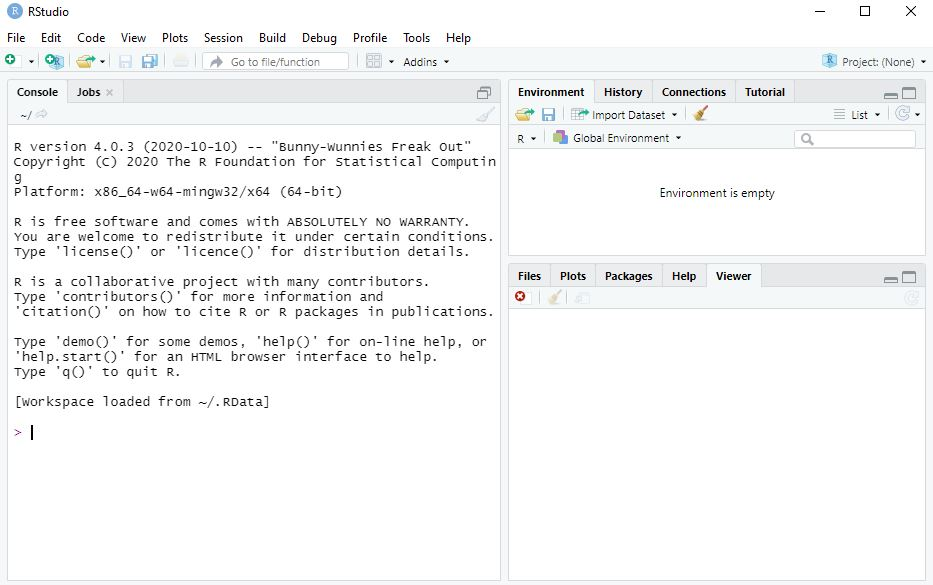
\includegraphics[width=12.96in]{img/Rstudiofig1}

Aquí vemos tres ventanas: a la izquierda \textbf{la consola} y a la derecha una ventana que dice \textbf{ambiente (environment)} arriba y \textbf{los visores} abajo.

La consola es nuestra comunicación más directa con R, cada línea que escribimos es leído por el programa como una solicitud y es ejecutado (y se devuelve el resultado) inmediatamente después de que presionamos ``enter''

Hagamos algunas pruebas:

\hypertarget{consola}{%
\section{Consola}\label{consola}}

\begin{enumerate}
\def\labelenumi{\arabic{enumi}.}
\tightlist
\item
  Escribamos en la consola algunas operaciones matemáticas (escribamos cada linea y damos enter para que nos devuelva el resultado)
\end{enumerate}

Sumemos y restemos por ejemplo:

\texttt{25+5}

\texttt{56-3}

Podemos hacer multiplicaciones y divisiones

\texttt{5*5} (para las multiplicaciones)

\texttt{25/5} (para las divisiones)

\begin{enumerate}
\def\labelenumi{\arabic{enumi}.}
\setcounter{enumi}{1}
\tightlist
\item
  Probemos ahora algo mas interesante:
\end{enumerate}

Preguntemosle a R si 25 es mayor que 50, para eso escribamos en la consola

\texttt{25\textgreater{}50}

O si 25 es exactamente igual a 5 por 5

\texttt{25==(5*5)}

En estos ejercicios hemos usado una notacion particular para \emph{pedirle cosas a R}, un breve resumen de esa \textbf{sintaxis} pueden verla en el siguiente enlace:
\url{https://www.statmethods.net/management/operators.html}

Prestemos atencion al segundo ejercicio, en estos ejercicios R nos devolvió un tipo de información distinta de la numérica, en este caso verdadero o falso (estas preguntas que hicimos se llaman \textbf{operadores lógicos} y devuelven este tipo de resultados)

\begin{enumerate}
\def\labelenumi{\arabic{enumi}.}
\setcounter{enumi}{2}
\tightlist
\item
  Hagamos algo más complicado, escribamos lo siguiente y veamos que pasa:
\end{enumerate}

\begin{Shaded}
\begin{Highlighting}[]
\FunctionTok{set.seed}\NormalTok{(}\DecValTok{123}\NormalTok{)}
\NormalTok{ejemplo }\OtherTok{\textless{}{-}} \FunctionTok{rnorm}\NormalTok{(}\AttributeTok{n =} \DecValTok{1000}\NormalTok{, }\AttributeTok{mean =} \DecValTok{2}\NormalTok{, }\AttributeTok{sd =} \DecValTok{35}\NormalTok{)}
\FunctionTok{hist}\NormalTok{(ejemplo, }\AttributeTok{col=}\StringTok{\textquotesingle{}grey\textquotesingle{}}\NormalTok{, }\AttributeTok{breaks=}\DecValTok{40}\NormalTok{, }
     \AttributeTok{ylab =} \StringTok{"Frecuencia"}\NormalTok{, }\AttributeTok{main =} \StringTok{"Nuestro primer histograma"}\NormalTok{)}
\end{Highlighting}
\end{Shaded}

Seguramente lo que obtenemos es algo así:

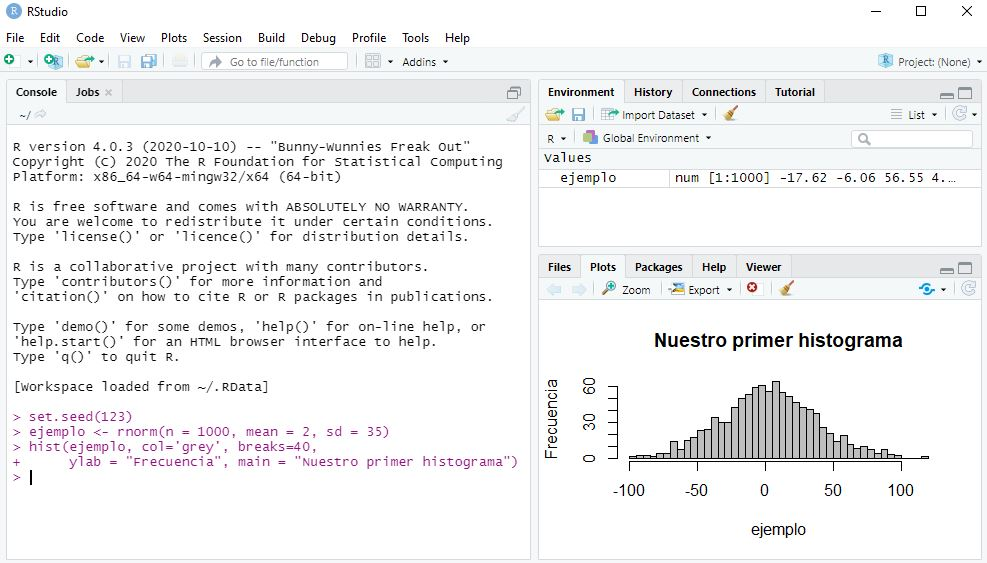
\includegraphics[width=13.71in]{img/Rstudiofig2}

Bueno creamos un histograma repasemos un poco lo que obtuvimos, esta vez el resultado no es presentado en la consola sino en el \textbf{visor} esto ocurre porque el resultado es un \textbf{render}.

Render es una palabra en inglés que vamos a utilizar para toda transformación de resultados en un contenido multimedia.

Si observamos la ventana de \emph{ambiente} vemos que apareció algo llamado ejemplo esto es un \textbf{objeto} que creamos con el código que usamos; en la siguiente sección hablaremos de los objetos. \emph{Recordemos que R es un lenguaje ``orientado a objetos'' así que estos son clave en el proceso}

\hypertarget{scripts}{%
\section{Scripts}\label{scripts}}

Si bien podemos trabajar comodamente en la consola esta conlleva algunas desventajas. En la consola no podemos editar nuestro código (cambiar o corregir aspectos) sin volver a escribirlo y no podemos guardarlo.
Para ello es que vamos a trabajar con scripts, archivos que podemos guardar, que se pueden volver a ejecutar y que sólo se ejecutan si nosotros lo solicitamos

\hypertarget{crear-un-script}{%
\subsection{Crear un script}\label{crear-un-script}}

Para crear un script debemos utilizar el menu desplegable \texttt{File} y seleccionar \texttt{New\ file} y ahi \texttt{R\ script}

Esto nos dará una configuración así:

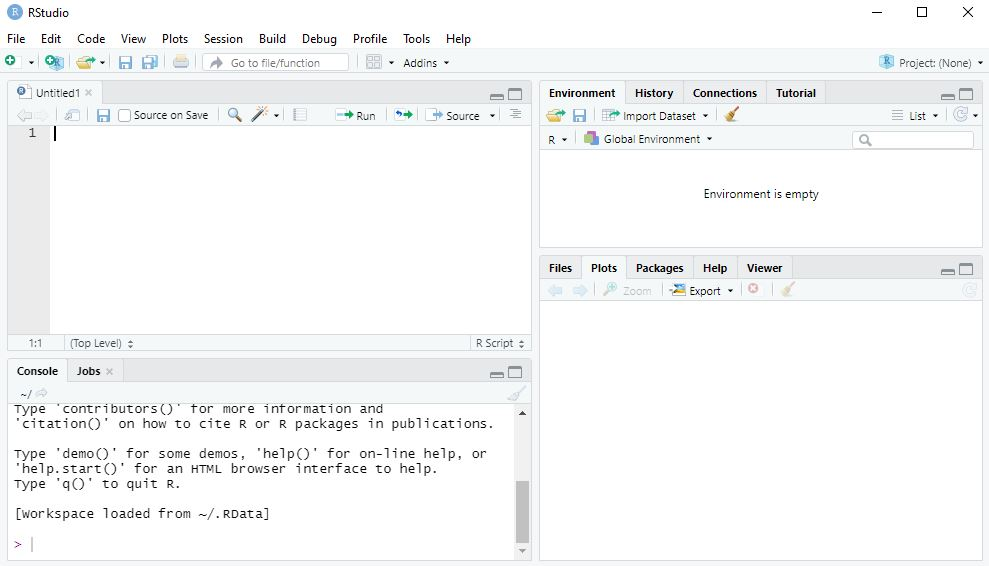
\includegraphics[width=13.74in]{img/Rstudiofig3}

Ahora tenemos un esquema en 4 ventanas, vamos a repasar que son y paraque las vamos a utilizar:

\begin{itemize}
\tightlist
\item
  \textbf{Script}: arriba y a la izquierda es donde escribiremos los comandos, funciona como un editor de texto. RStudio para hacernos la tarea más fácil tiene un texto predictivo que nos sugiere las funciones a medida que las usemos. Nuestros comandos solo se ejecutaran si presionamos el botón \texttt{run} (en la misma ventana) o si presionamos \texttt{Ctrl}+`\texttt{Enter}, sólo se ejecutaran las líneas que seleccionemos (que se seleccionan como si fueran un editor de texto)
\item
  \textbf{Environment}: el ambiente de trabajo, aquí nos mostrarà que objetos existen y podemos manipular -aquì apareceran por ejemplo las bases de datos con las que trabajemos
\item
  \textbf{Consola}: la consola sigue habilitada para escribir pero (como vimos que esto no es muy cómodo) vamos a dejar que el script le pida cosas a la consola cada vez que lo ejecutemos, de ahora en más la consola \_sólo nos mostrará los resultados que sean sólo números o texto (y también las advertencias o mensajes de error que tenga para informarnos)
\item
  \textbf{Visor}: en el visor aparecerán todos los contenidos multimedia que genere (los renders), hay botones en el visor que nos permitirá exportar estas imagenes o editarlas
\end{itemize}

\hypertarget{objetos}{%
\section{Objetos}\label{objetos}}

Como repetimos varias veces \textbf{R es un lenguaje orientado a objetos.}
Los objetos en si son como contenedores, en donde se puede alojar un valor aislado, o una lista de valores por ejemplo.
La clave de ello es que en R podemos manipular ese objeto y con ello todo su contenido. Los objetos se manipulan a través de \textbf{funciones}

\hypertarget{creaciuxf3n-de-objetos}{%
\subsection{Creación de objetos}\label{creaciuxf3n-de-objetos}}

Vamos a crear algunos objetos, corramos los siguientes comandos en R:

\begin{Shaded}
\begin{Highlighting}[]
\CommentTok{\#Creamos el objeto a}

\NormalTok{a}\OtherTok{\textless{}{-}}\DecValTok{5}

\CommentTok{\#El objeto a ahora debería aparecer en el Environment}
\CommentTok{\#Si queremos ver el contenido del objeto hay tres opciones:}

\CommentTok{\#1. lo muestra en la consola}
\NormalTok{a }
\CommentTok{\#2. le aplica una función "imprimir en la consola" a todo el objeto a}
\FunctionTok{print}\NormalTok{(a) }
\CommentTok{\#3. la tercer opcion es hacer doble clic en el objeto en el Environment}
\end{Highlighting}
\end{Shaded}

\begin{quote}
\textbf{Aclaración}: El código presentado después de \textbf{\#} se llama \textbf{comentario}, no se ejecuta y no es necesario escribirlo. Simplemente son notas que a veces dejamos para entender o aclarar algo del código.
Tambien podemos usar \textbf{\#} para inahbilitar temporalmente algunas lìneas del código (es muy útil cuando buscamos errores)
\end{quote}

Habrá notado que para crear un objeto basta con ponerle un nombre (alfanumerico sin espacios) y asignarle un contenido. Para asignarle un contenido usamos el operador \textbf{asiganción} o sea \texttt{\textless{}-}. Este símbolo puedecambiar de dirección: \texttt{\textless{}-} o \texttt{-\textgreater{}}. \emph{Siempre la flecha va de contenido al nombre del objeto}, siguiendo esta regla:

\texttt{nombre\_del\_objeto\ \textless{}-\ valor\_del\_objeto}

\hypertarget{ejercicios}{%
\subsubsection{\texorpdfstring{ Ejercicios}{ Ejercicios}}\label{ejercicios}}

Hasta ahora hemos creado objetos de un solo contenido, vamos a crear objetos con contenidos mas diversos. Escribamos el siguiente codigo en R

\begin{Shaded}
\begin{Highlighting}[]
\CommentTok{\#Crea un objeto con numeros del uno al 10}
\NormalTok{numeros}\OtherTok{\textless{}{-}}\DecValTok{1}\SpecialCharTok{:}\DecValTok{10}

\CommentTok{\#Crea un objeto que contiene una lista de nombres}
\NormalTok{nombres}\OtherTok{\textless{}{-}}\FunctionTok{c}\NormalTok{(}\StringTok{"Ismael"}\NormalTok{, }\StringTok{"Claudia"}\NormalTok{, }\StringTok{"Alberto"}\NormalTok{, }\StringTok{"Juan Carlos"}\NormalTok{, }\StringTok{"Laura"}\NormalTok{, }\StringTok{"José"}\NormalTok{, }\StringTok{"Luis"}\NormalTok{, }\StringTok{"Lorena"}\NormalTok{, }\StringTok{"Charly"}\NormalTok{, }\StringTok{"Fito"}\NormalTok{)}

\CommentTok{\#Creemos un objeto que contenga la lista del genero }
\CommentTok{\#de los primeros  alumnos del curso}

\NormalTok{genero}\OtherTok{\textless{}{-}}\FunctionTok{c}\NormalTok{(}\StringTok{"varon"}\NormalTok{, }\StringTok{"mujer"}\NormalTok{,}\StringTok{"varon"}\NormalTok{,}\StringTok{"varon"}\NormalTok{, }\StringTok{"mujer"}\NormalTok{,}\StringTok{"varon"}\NormalTok{, }\StringTok{"varon"}\NormalTok{, }\StringTok{"mujer"}\NormalTok{,}\StringTok{"varon"}\NormalTok{,}\StringTok{"varon"}\NormalTok{)}


\DocumentationTok{\#\#Ahora imprimamoslo para ver su contenido}

\FunctionTok{print}\NormalTok{(numeros)}
\end{Highlighting}
\end{Shaded}

\begin{verbatim}
##  [1]  1  2  3  4  5  6  7  8  9 10
\end{verbatim}

\begin{Shaded}
\begin{Highlighting}[]
\FunctionTok{print}\NormalTok{(nombres)}
\end{Highlighting}
\end{Shaded}

\begin{verbatim}
##  [1] "Ismael"      "Claudia"     "Alberto"     "Juan Carlos" "Laura"      
##  [6] "José"        "Luis"        "Lorena"      "Charly"      "Fito"
\end{verbatim}

\begin{Shaded}
\begin{Highlighting}[]
\FunctionTok{print}\NormalTok{(genero)}
\end{Highlighting}
\end{Shaded}

\begin{verbatim}
##  [1] "varon" "mujer" "varon" "varon" "mujer" "varon" "varon" "mujer" "varon"
## [10] "varon"
\end{verbatim}

Vamos a aclarar algunos conceptos de la sintaxis:

\begin{enumerate}
\def\labelenumi{\arabic{enumi}.}
\tightlist
\item
  Usamos \texttt{:} entre dos numeros para decirle a R que nos de todos los numeros en ese rango inclusive los extremos.
\item
  Cuando creamos objetos llenos de texto, como los nombres o el genero, R no entiende de palabras entonces debemos aclararlo para eso los escribimos entre \texttt{""}. Esto dice a R donde empieza y termina una palabra y que es sólo eso (porque a veces las palabras son objetos o funciones, pero entre comillas es solo una palabra). Si queremos incluir una enumeracion de palabras o de objetos de distinta clase debemos usar la sintaxis \texttt{c(contenido1,\ contenido2,\ contenido3)}
\end{enumerate}

\hypertarget{clases-de-objetos}{%
\subsection{Clases de objetos}\label{clases-de-objetos}}

Veamos después de nuestro ejercicio que pasó en el Environment, seguro tenemos algo así:

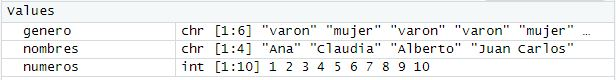
\includegraphics[width=8.56in]{img/Rstudiofig4}

Vemos que aparecen nuestros objetos, seguidos por tres letras que hablan de la \textbf{clase} a la que pertenece (tranquilos que hablaremos de ello más adelante), después vemos dos numeros entre corchetes, estos son la \textbf{dimensión} de nuestro objeto.

Para R los objetos son \textbf{matrices}, es decir distribuciones en dos dimensiones (como filas y columnas) de los contenidos, que en matrices se dice \emph{n x m}. N tradicionalmente habla de el numero de filas y m del numero de columnas.

Para una revisión de lo que es una matriz pueden visitar \url{https://es.wikipedia.org/wiki/Matriz_(matem\%C3\%A1ticas)}

Esta forma de entender los datos es muy útil porque las bases de datos son (en definitiva) matrices con contenido numerico o algebraico.

Volviendo a la ventana de R, nuestros objetos son descriptos como {[}1:6{]} o {[}1:10{]}, eso quiere decir que son matrices con una sola fila. A este tipo especial de matrices lo llamamos \textbf{vectores}.

Pese a que estemos en los primeros pasos y todo parezca muy abstracto hagamos un ejercicio de extrapolación, nuestros vectores (matrices de una sola dimension) pueden funcionar como columnas de una bazse de datos y la base de datos una matriz mas grande que se forma mezclando los vectores. Sí suena muy loco, pero confiemos que se va a ir aclarando.

Los vectores pueden tener distinto contenido, la \textbf{clase} de un vector es definida por su contenido. En reglas generales los vectores pueden adoptar la siguientes clases:
R tiene cinco clases básicas de vectores:

\begin{itemize}
\tightlist
\item
  character (letras)
\item
  numeric (números enteros unicamente)
\item
  integer (números reales, o sea con decimales)
\item
  complex (números complejos)
\item
  logical (verdadero/falso o True/False)
\end{itemize}

Si queremos ver de que clase es un objeto podemos aplicarle la función \texttt{class()}

Hagamos el ejercicio con nuestros objetos:

\begin{Shaded}
\begin{Highlighting}[]
\FunctionTok{class}\NormalTok{(numeros)}
\end{Highlighting}
\end{Shaded}

\begin{verbatim}
## [1] "integer"
\end{verbatim}

\begin{Shaded}
\begin{Highlighting}[]
\FunctionTok{class}\NormalTok{(nombres)}
\end{Highlighting}
\end{Shaded}

\begin{verbatim}
## [1] "character"
\end{verbatim}

\begin{Shaded}
\begin{Highlighting}[]
\FunctionTok{class}\NormalTok{(genero)}
\end{Highlighting}
\end{Shaded}

\begin{verbatim}
## [1] "character"
\end{verbatim}

Presten atención que el nombre de los objetos \textbf{NO} llevan comillas porque queremos que R entienda que es el objeto números y no la palabra ``números'' por ejemplo

Desafío:
Corran los siguientes comandos en su script

\texttt{print(numeros)}

\texttt{print("numeros")}

¿Notan la diferencia de resultados? Prepárense para explicar en clase por qué

\begin{Shaded}
\begin{Highlighting}[]
\CommentTok{\#Los objetos pueden tener contendio mixto pero reciben la clase del tipo menos informativo que contengan por ejemplo:}

\NormalTok{mixto}\OtherTok{\textless{}{-}}\FunctionTok{c}\NormalTok{(}\StringTok{"Ismael"}\NormalTok{, }\DecValTok{1}\NormalTok{, }\FloatTok{1.33}\NormalTok{)}

\CommentTok{\#Este es un objeto con contenido numeric, integer y character}

\FunctionTok{class}\NormalTok{(mixto)}
\end{Highlighting}
\end{Shaded}

\begin{verbatim}
## [1] "character"
\end{verbatim}

Lo que hemos hecho recién es aplicar intuitivamente una \textbf{función} a un objeto. Este sencillo acto es la mayor complejidad que tiene R, todo, todo se trata de esto

Existe un 6to. tipo de vectores que nos serán muy pero muy útil, el \textbf{factor}. Los factores son grupos de datos categóricos (son palabras para R) pero que albergam un orden intrínseco: ``Grande'', ``mediano'' y ``chico'', por ejemplo. Para crearlos no basta informarle a R su contenido, sino que tambien hay que indicar el orden de jerarquia de los valores

\begin{Shaded}
\begin{Highlighting}[]
\CommentTok{\#este objeto se crea con dos vectores, un vector con los valores de los alumnos y un vector con el orden de los niveles}
\NormalTok{altura\_alumnos }\OtherTok{\textless{}{-}} \FunctionTok{factor}\NormalTok{(}\FunctionTok{c}\NormalTok{(}\StringTok{"alto"}\NormalTok{, }\StringTok{"bajo"}\NormalTok{, }\StringTok{"bajo"}\NormalTok{, }\StringTok{"mediano"}\NormalTok{,}\StringTok{"bajo"}\NormalTok{, }\StringTok{"alto"}\NormalTok{, }\StringTok{"bajo"}\NormalTok{, }\StringTok{"bajo"}\NormalTok{, }\StringTok{"mediano"}\NormalTok{,}\StringTok{"bajo"}\NormalTok{),}
                       \AttributeTok{levels=}\FunctionTok{c}\NormalTok{(}\StringTok{"bajo"}\NormalTok{, }\StringTok{"mediano"}\NormalTok{, }\StringTok{"alto"}\NormalTok{))}
\end{Highlighting}
\end{Shaded}

Si lo miramos en el environment:

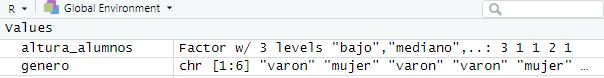
\includegraphics[width=8.39in]{img/Rstudiofig5}

Nos dice que es un factor que tiene tres niveles y vemos que al valor real de cada alumno lo convirtió en un número que representa el nivel.

Esto es muy útil porque mucho de nuestros datos pueden presentarse de esta forma

\hypertarget{operaciones-con-objetos}{%
\subsection{Operaciones con objetos}\label{operaciones-con-objetos}}

Los objetos se pueden manipular con operaciones como hemos visto previamente, tengan uno o muchos elementos

\begin{Shaded}
\begin{Highlighting}[]
\CommentTok{\#Quiero dividir todos los elementos del vector numeros a la mitad}

\NormalTok{numeros}\SpecialCharTok{/}\DecValTok{2}
\end{Highlighting}
\end{Shaded}

\begin{verbatim}
##  [1] 0.5 1.0 1.5 2.0 2.5 3.0 3.5 4.0 4.5 5.0
\end{verbatim}

\begin{Shaded}
\begin{Highlighting}[]
\CommentTok{\# Si quisieramos usar esta lista que hemos obtenido ahora màs adelante la podemos asignar a otro objeto}

\NormalTok{numeros\_divididos}\OtherTok{\textless{}{-}}\NormalTok{numeros}\SpecialCharTok{/}\DecValTok{2}

\CommentTok{\#Fijense que ahora existe en el environment}
\FunctionTok{print}\NormalTok{(numeros\_divididos)}
\end{Highlighting}
\end{Shaded}

\begin{verbatim}
##  [1] 0.5 1.0 1.5 2.0 2.5 3.0 3.5 4.0 4.5 5.0
\end{verbatim}

\begin{Shaded}
\begin{Highlighting}[]
\CommentTok{\#podemos hacer muchas cosas con los operadores, como operaciones complejas}

\NormalTok{(numeros}\SpecialCharTok{/}\DecValTok{2}\NormalTok{)}\SpecialCharTok{+}\DecValTok{1}
\end{Highlighting}
\end{Shaded}

\begin{verbatim}
##  [1] 1.5 2.0 2.5 3.0 3.5 4.0 4.5 5.0 5.5 6.0
\end{verbatim}

\begin{Shaded}
\begin{Highlighting}[]
\CommentTok{\#ahora a cada componente lo dividimos por la mitad y le sumamos uno}
\end{Highlighting}
\end{Shaded}

También podemos hacer operaciones con vectores de palabras.

\begin{Shaded}
\begin{Highlighting}[]
\CommentTok{\#queremos saber si el contenido de la lista genero es varon por ejemplo}

\NormalTok{genero }\SpecialCharTok{==} \StringTok{"varon"}
\end{Highlighting}
\end{Shaded}

\begin{verbatim}
##  [1]  TRUE FALSE  TRUE  TRUE FALSE  TRUE  TRUE FALSE  TRUE  TRUE
\end{verbatim}

\begin{Shaded}
\begin{Highlighting}[]
\CommentTok{\# Ahora obtuvimos un vector del tipo "lógico" porque aplicamos un operador logico y este es su resultado}
\end{Highlighting}
\end{Shaded}

\begin{Shaded}
\begin{Highlighting}[]
\CommentTok{\#Un dato relevante es que la clase True o False puede usarse en operaciones numericas (True es igual a 1 y False es igual a 0), por eso a este vector logico podemos sumarle 1}
\NormalTok{genero\_TF}\OtherTok{\textless{}{-}}\NormalTok{genero }\SpecialCharTok{==} \StringTok{"varon"}
\FunctionTok{class}\NormalTok{(genero\_TF)}
\end{Highlighting}
\end{Shaded}

\begin{verbatim}
## [1] "logical"
\end{verbatim}

\begin{Shaded}
\begin{Highlighting}[]
\NormalTok{genero\_TF}\SpecialCharTok{+}\DecValTok{1}
\end{Highlighting}
\end{Shaded}

\begin{verbatim}
##  [1] 2 1 2 2 1 2 2 1 2 2
\end{verbatim}

\hypertarget{funciones-con-objetos}{%
\subsection{Funciones con objetos}\label{funciones-con-objetos}}

A los objetos se les pueden aplicar funciones (intuitivamente ya hemos usado \texttt{class()} y \texttt{print()}). El numero de funciones es enorme, veamos algunos ejemplos.

\begin{Shaded}
\begin{Highlighting}[]
\CommentTok{\#queremos contar el numero de elementos que hay en el objeto genero}

\FunctionTok{length}\NormalTok{(genero)}
\end{Highlighting}
\end{Shaded}

\begin{verbatim}
## [1] 10
\end{verbatim}

\begin{Shaded}
\begin{Highlighting}[]
\CommentTok{\#esta funcion nos da el "largo" del vector, es decir el numero maximo de elementos}
\end{Highlighting}
\end{Shaded}

\begin{Shaded}
\begin{Highlighting}[]
\CommentTok{\#tambien existen funciones para "cambiar" la clase de un objeto}
\CommentTok{\#supongamos que queremos que al leer el vector número, R no lo entienda como numeros sino como palabras}

\NormalTok{numeros\_como\_palabras}\OtherTok{\textless{}{-}}\FunctionTok{as.character}\NormalTok{(numeros)}

\FunctionTok{class}\NormalTok{(numeros\_como\_palabras)}
\end{Highlighting}
\end{Shaded}

\begin{verbatim}
## [1] "character"
\end{verbatim}

\begin{Shaded}
\begin{Highlighting}[]
\CommentTok{\#Probemos ejecutar el siguiente comando }

\NormalTok{numeros\_como\_palabras}\SpecialCharTok{+}\DecValTok{1}
\end{Highlighting}
\end{Shaded}

El resultado es algo así

Error in numeros\_como\_palabras + 1 :
non-numeric argument to binary operator

\begin{Shaded}
\begin{Highlighting}[]
\CommentTok{\#pero en este caso podemos revertir el rpoblema con una funcion}

\NormalTok{numeros\_como\_palabras}\OtherTok{\textless{}{-}}\FunctionTok{as.numeric}\NormalTok{(numeros\_como\_palabras)}

\CommentTok{\#notese que asignamos un objeto transformado al mismo objeto, esta operacion "sobrescribe el objeto", no es aconsejable porque es irreversible (aqui la usamos para no generar miles de objetos)}

\FunctionTok{class}\NormalTok{(numeros\_como\_palabras)}
\end{Highlighting}
\end{Shaded}

\begin{verbatim}
## [1] "numeric"
\end{verbatim}

\begin{Shaded}
\begin{Highlighting}[]
\CommentTok{\#ahora no hay problema con la suma}

\NormalTok{numeros\_como\_palabras}\SpecialCharTok{+}\DecValTok{1}
\end{Highlighting}
\end{Shaded}

\begin{verbatim}
##  [1]  2  3  4  5  6  7  8  9 10 11
\end{verbatim}

\begin{Shaded}
\begin{Highlighting}[]
\CommentTok{\#estas funciones de asignacion de clase no siempre se pueden usar, no podemos convertir los nombres en numeros porque no conocemos a que numero asignarlos por ejemplo}

\NormalTok{nombres\_como\_numeros}\OtherTok{\textless{}{-}}\FunctionTok{as.numeric}\NormalTok{(nombres)}
\end{Highlighting}
\end{Shaded}

\begin{verbatim}
## Warning: NAs introduced by coercion
\end{verbatim}

\begin{Shaded}
\begin{Highlighting}[]
\CommentTok{\#nos da un mensaje de error, veamos que pasó}
\end{Highlighting}
\end{Shaded}

\begin{Shaded}
\begin{Highlighting}[]
\CommentTok{\#la clase se asignó}
\FunctionTok{class}\NormalTok{(nombres\_como\_numeros)}
\end{Highlighting}
\end{Shaded}

\begin{verbatim}
## [1] "numeric"
\end{verbatim}

\begin{Shaded}
\begin{Highlighting}[]
\CommentTok{\#pero los objetos no pudieron convertirse, entonces se convirtieron en NA, que es el equivalente a un valor perdido}

\FunctionTok{print}\NormalTok{(nombres\_como\_numeros)}
\end{Highlighting}
\end{Shaded}

\begin{verbatim}
##  [1] NA NA NA NA NA NA NA NA NA NA
\end{verbatim}

\begin{Shaded}
\begin{Highlighting}[]
\CommentTok{\#si queremos calcular por ejemplo la media de nuestro vector números}

\FunctionTok{mean}\NormalTok{(numeros)}
\end{Highlighting}
\end{Shaded}

\begin{verbatim}
## [1] 5.5
\end{verbatim}

\begin{Shaded}
\begin{Highlighting}[]
\CommentTok{\#O el Desvío estándard por ejemplo}

\FunctionTok{sd}\NormalTok{(numeros)}
\end{Highlighting}
\end{Shaded}

\begin{verbatim}
## [1] 3.02765
\end{verbatim}

FELICITACIONES HA HECHO SU PRIMER ANÁLISIS DE ESTADÍSTICA DESCRIPTIVA EN R

\hypertarget{ejercicio-integrador}{%
\section{\texorpdfstring{ Ejercicio integrador}{ Ejercicio integrador}}\label{ejercicio-integrador}}

Continuemos con nuestro esfuerzo de abstracción y volvamos a pensar en las bases de datos como matrices.

Una columna de una variable es entonces un vector, y los valores que adopta en cada sujeto sus componentes.

\begin{enumerate}
\def\labelenumi{\arabic{enumi}.}
\tightlist
\item
  ¿Que clase de vector serían las siguientes variables:?
\end{enumerate}

\begin{quote}
\textbf{Tipo de variables}\_\_\_\_\_\_\_\_\_\_\_\_\_\_\_\textbf{Clase del vector}

Variable continua

Variables dicotómica

Variable ordinal

Variable categorica
\end{quote}

\begin{enumerate}
\def\labelenumi{\arabic{enumi}.}
\setcounter{enumi}{1}
\tightlist
\item
  Ahora apliquemos lo aprendido a conceptos de ``la vida real'', dados estos ejemplos de variables trate de clasificarlos con la definición teórica y en la clase de vector que se transformaría
\end{enumerate}

\begin{quote}
\textbf{Tipo de variables}\_\_\_\_\_\_\_\_\_\_\textbf{Tipo de variable}\_\_\_\_\_\_\_\_\_\_\textbf{Clase del vector}

Edad (en años)

Sexo

Nota de un examen

Temperatura corporal de un castor (ºC)

Coeficiente de inteligencia (IQ)

Color de ojos

Ocurrencia de un evento o no

Medalla olimpica obtenida

Estrellas en mercado libre
\end{quote}

Recuerden un principio esencial en la operacionalización de las variables:


\includegraphics[width=7.71in]{img/chiquita}

Las variables pueden cambiar de categoría si decidimos ``verlas'' de una forma u otra, pero esto afecta a la forma que se las ``trata'' (la clase que R les asigna y eso determina que operaciones podemos hacer con ellas)

\hypertarget{dataset-dataframe-bases-de-datos}{%
\section{Dataset-Dataframe, bases de datos}\label{dataset-dataframe-bases-de-datos}}

Bueno ha llegado el momento de dejar los cielos de la abstracción y pasar de los vectores y las matrices a las bases de datos.

En esta sección vamos a ver como podemos construir un conjunto de datos a partir de objetos.

Si bien existen sutiles diferencias en los términos dataset y dataframe son dos términos sinónimos a los efectos de este curso y hablan de un conjunto de datos que podemos manipular en R

Recordemos que tenemos nuestros objetos previamente creados

\begin{Shaded}
\begin{Highlighting}[]
\NormalTok{genero}
\end{Highlighting}
\end{Shaded}

\begin{verbatim}
##  [1] "varon" "mujer" "varon" "varon" "mujer" "varon" "varon" "mujer" "varon"
## [10] "varon"
\end{verbatim}

\begin{Shaded}
\begin{Highlighting}[]
\NormalTok{nombres}
\end{Highlighting}
\end{Shaded}

\begin{verbatim}
##  [1] "Ismael"      "Claudia"     "Alberto"     "Juan Carlos" "Laura"      
##  [6] "José"        "Luis"        "Lorena"      "Charly"      "Fito"
\end{verbatim}

\begin{Shaded}
\begin{Highlighting}[]
\NormalTok{numeros}
\end{Highlighting}
\end{Shaded}

\begin{verbatim}
##  [1]  1  2  3  4  5  6  7  8  9 10
\end{verbatim}

\begin{Shaded}
\begin{Highlighting}[]
\DocumentationTok{\#\#Si ya no los tienen en su ambiente, vuelvan a correr el código donde los creamos anteriormente}
\end{Highlighting}
\end{Shaded}

Vamos a crear un nuevo objeto vector que va a contener numeros al azar entre 0 y 10

\begin{Shaded}
\begin{Highlighting}[]
\FunctionTok{set.seed}\NormalTok{(}\DecValTok{123}\NormalTok{) }
\DocumentationTok{\#\#usamos este comando para que (pese a que se haga al azar) todos podamos obtener el mismo resultado}

\NormalTok{peso\_alumnos }\OtherTok{\textless{}{-}} \FunctionTok{runif}\NormalTok{(}\AttributeTok{n=}\DecValTok{10}\NormalTok{, }\AttributeTok{min=}\DecValTok{50}\NormalTok{, }\AttributeTok{max=}\DecValTok{100}\NormalTok{) }
\CommentTok{\#acá usamos una función para generar números aleatorios}
\CommentTok{\#el primer valor es la cantidad de numeros, y los otros dos el minimo y el máximo}
\end{Highlighting}
\end{Shaded}

\begin{quote}
Todas las funciones necesitan información para trabajar, esa información agregada por el usuario se llaman \textbf{parámetros} y a la forma en que se cargan \textbf{argumento}. Cada función tiene sus propias reglas (pero generalmente son parecidas). A esto es lo que llamamos \textbf{sintaxis}. RStudio tiende a sugerirnos la sintaxis necesaria (prueben a ir escribiendo despacio la función y verán aparecer el predictivo)
Si no conocemos la sintaxis de una función podemos usar la función: \texttt{help()}

Prueben a tipear \texttt{help(runif)} y veran un documento detallado sobre como utilizarla
\end{quote}

\hypertarget{creaciuxf3n-de-base-de-datos}{%
\subsection{Creación de base de datos:}\label{creaciuxf3n-de-base-de-datos}}

Vamos a ver una nueva función que trabaja con vectores, la función \texttt{data.frame()}.
Apliquemosla a nuestros objetos de la siguiente manera:

\begin{Shaded}
\begin{Highlighting}[]
\NormalTok{mi\_primera\_base}\OtherTok{\textless{}{-}}\FunctionTok{data.frame}\NormalTok{(numeros, nombres, genero, altura\_alumnos, peso\_alumnos)}
\end{Highlighting}
\end{Shaded}

FELICITACIONES CREAMOS UNA BASE DE DATOS A PUNTO DE PARTIDA DE UN CONJUNTO DE VECTORES

Para hacer esto usamos la función data.frame(), los \emph{argumentos} que esta función necesita es solamente el nombre de los vectores en el orden que lo queremos.

Veamos que pasó en el Enviroment:

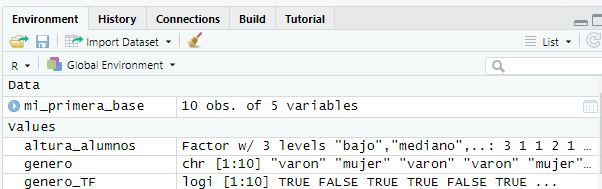
\includegraphics[width=8.36in]{img/Rstudiofig6}

Ahora tenemos por separado nuestra base, nos dice el numero de observaciones, que corresponde al largo de los vectores y el número de variables (que es el número de vectores que incluímos)

Si hacemos clic sobre el boton celeste con el signo play podemos ver la forma de la base.

\hypertarget{funciones-buxe1sicas-para-los-dataframes}{%
\subsection{Funciones básicas para los dataframes}\label{funciones-buxe1sicas-para-los-dataframes}}

Exporemos algunas funciones que se pueden aplicar a este objeto.
Vamos con la función querida función \texttt{class()}

\begin{Shaded}
\begin{Highlighting}[]
\FunctionTok{class}\NormalTok{(mi\_primera\_base)}
\end{Highlighting}
\end{Shaded}

\begin{verbatim}
## [1] "data.frame"
\end{verbatim}

Nuestra base es un obejto de R de la clase \textbf{dataframe}, esta es una clase de objeto especial que si bien como veníamos mencionando es como una matriz, esta tiene encabezados.

Probemos algunas funciones simples.

\begin{enumerate}
\def\labelenumi{\arabic{enumi}.}
\tightlist
\item
  La función \texttt{head()}, nos muestra los primeros valores de la base
\end{enumerate}

\begin{Shaded}
\begin{Highlighting}[]
\FunctionTok{head}\NormalTok{(mi\_primera\_base)}
\end{Highlighting}
\end{Shaded}

\begin{verbatim}
##   numeros     nombres genero altura_alumnos peso_alumnos
## 1       1      Ismael  varon           alto     64.37888
## 2       2     Claudia  mujer           bajo     89.41526
## 3       3     Alberto  varon           bajo     70.44885
## 4       4 Juan Carlos  varon        mediano     94.15087
## 5       5       Laura  mujer           bajo     97.02336
## 6       6        José  varon           alto     52.27782
\end{verbatim}

Por default nos muestra los primeros 6 elementos, pero podemos introducirle parámetros para modificarla

\begin{Shaded}
\begin{Highlighting}[]
\FunctionTok{head}\NormalTok{(mi\_primera\_base, }\DecValTok{3}\NormalTok{)}
\end{Highlighting}
\end{Shaded}

\begin{verbatim}
##   numeros nombres genero altura_alumnos peso_alumnos
## 1       1  Ismael  varon           alto     64.37888
## 2       2 Claudia  mujer           bajo     89.41526
## 3       3 Alberto  varon           bajo     70.44885
\end{verbatim}

El argumento que le agregamos es el número de filas que queremos que nos muestre.

Esta función es muy útil cuando queremos dar un vistazo preliminar a una base muy grande que tarda mucho tiempo en cargar.

\begin{enumerate}
\def\labelenumi{\arabic{enumi}.}
\setcounter{enumi}{1}
\tightlist
\item
  La función \texttt{tail()} . Probemos otra similar para previsualizar la base de datos.
\end{enumerate}

\begin{Shaded}
\begin{Highlighting}[]
\FunctionTok{tail}\NormalTok{(mi\_primera\_base)}
\end{Highlighting}
\end{Shaded}

\begin{verbatim}
##    numeros nombres genero altura_alumnos peso_alumnos
## 5        5   Laura  mujer           bajo     97.02336
## 6        6    José  varon           alto     52.27782
## 7        7    Luis  varon           bajo     76.40527
## 8        8  Lorena  mujer           bajo     94.62095
## 9        9  Charly  varon        mediano     77.57175
## 10      10    Fito  varon           bajo     72.83074
\end{verbatim}

Sin usar grandes poderes de deducción nos damos cuenta que muestra los últimos elementos de la base.

\begin{enumerate}
\def\labelenumi{\arabic{enumi}.}
\setcounter{enumi}{2}
\tightlist
\item
  Veamos una función muy necesaria, la función \texttt{str()}:
\end{enumerate}

\begin{Shaded}
\begin{Highlighting}[]
\FunctionTok{str}\NormalTok{(mi\_primera\_base)}
\end{Highlighting}
\end{Shaded}

\begin{verbatim}
## 'data.frame':    10 obs. of  5 variables:
##  $ numeros       : int  1 2 3 4 5 6 7 8 9 10
##  $ nombres       : chr  "Ismael" "Claudia" "Alberto" "Juan Carlos" ...
##  $ genero        : chr  "varon" "mujer" "varon" "varon" ...
##  $ altura_alumnos: Factor w/ 3 levels "bajo","mediano",..: 3 1 1 2 1 3 1 1 2 1
##  $ peso_alumnos  : num  64.4 89.4 70.4 94.2 97 ...
\end{verbatim}

Esta función es sencillamente genial, nos devuelve un panorama general de la base, el numero de observaciones, las variables y una descripción de la clase de cada vector que la compone.

\begin{enumerate}
\def\labelenumi{\arabic{enumi}.}
\setcounter{enumi}{3}
\tightlist
\item
  Una función que siempre tiene que estar en nuestra caja de herramientas es la función \texttt{summary()}
\end{enumerate}

\begin{Shaded}
\begin{Highlighting}[]
\FunctionTok{summary}\NormalTok{(mi\_primera\_base)}
\end{Highlighting}
\end{Shaded}

\begin{verbatim}
##     numeros        nombres             genero          altura_alumnos
##  Min.   : 1.00   Length:10          Length:10          bajo   :6     
##  1st Qu.: 3.25   Class :character   Class :character   mediano:2     
##  Median : 5.50   Mode  :character   Mode  :character   alto   :2     
##  Mean   : 5.50                                                       
##  3rd Qu.: 7.75                                                       
##  Max.   :10.00                                                       
##   peso_alumnos  
##  Min.   :52.28  
##  1st Qu.:71.04  
##  Median :76.99  
##  Mean   :78.91  
##  3rd Qu.:92.97  
##  Max.   :97.02
\end{verbatim}

Esta función nos ha resuelto la tabla 1 de cualquier paper, si observan ha sacado estadísticos de resumen para variables continuas (numero y peso alumnos) y estadisticos de frecuencia para las variables nominales. Solo ha calculado el n de las variables que dejamos como ``palabras'' porque no le asignamos una mejor clase.

Como ven aquí se hace muy clara la necesidad de asignar la mejor clase posible a la variable para que R la trate apropiadamente.

Bueno como hemos visto, es posible crear una base desde la creación de vectores.Cómo todos estarán pensando, la toma de datos y la construcción de una base de esta forma es muy engorrosa, y lo es.

De ahora en mas vamos a trabajar utilizando bases de datos creadas en otros programas como Excel.


\includegraphics[width=10in]{img/pollilla}

\hypertarget{ejercicio-integrador-1}{%
\section{\texorpdfstring{ Ejercicio integrador}{ Ejercicio integrador}}\label{ejercicio-integrador-1}}

Vamos a cerrar esta unidad armando nuestro propio diccionario de funciones. Describa que tareas realizan estas funciones

\begin{quote}
\textbf{DICCIONARIO DE FUNCIONES}

print()

class()

as.numeric()

as.character()

is.numeric()

is.logical()

length()

mean()

sd()

help()

data.frame()

head()

tail()

str()

summary()
\end{quote}

Hay algunas funciones que no figuran en el texto, pero usted tiene funciones que le ayudaran a resolver ese problema

\hypertarget{ambientes-de-trabajo-y-manipulaciuxf3n-de-variables-i}{%
\chapter{Ambientes de trabajo y manipulación de variables (I)}\label{ambientes-de-trabajo-y-manipulaciuxf3n-de-variables-i}}

\hypertarget{antes-de-empezar}{%
\section{Antes de empezar}\label{antes-de-empezar}}

Una parte importante del trabajo en estadística depende de la prolijidad y el orden. Cualquier proyecto debe seguir estos pasos antes de empezar:

\begin{enumerate}
\def\labelenumi{\arabic{enumi}.}
\tightlist
\item
  Cree una carpeta destinada \textbf{sólo} al proyecto estadístico
\item
  Coloque el archivo de la base de datos (CSV, XLS, o el formato que prefiera en la carpeta)
\item
  Cree un script vacío de R y guárdelo en la carpeta
\item
  Establezca esa carpeta como su directorio de trabajo o \textbf{working directory}
\end{enumerate}

\hypertarget{directorio-de-trabajo-o-working-directory}{%
\section{Directorio de trabajo o Working directory}\label{directorio-de-trabajo-o-working-directory}}

En ocasiones R tiene que buscar archivos en una carpeta (por ejemplo cuando queremos que ``lea'' una base de datos que tenes en Excel) y en otras ocasiones va a necesitar guardar datos en una carpeta.

El lugar en donde haga ello se llama directorio de trabajo o \textbf{working directory}.

Si establecemos ese directorio de trabajo en la carpeta que creamos antes de empezar, R va a poder leer los datos de allí y guardarnos los resultados en el mismo lugar. Al final del día vamos a tener, la base, el script y los resultados prolijos y ordenados en el mismo lugar.

Vamos a aprender como establecer ese directorio.

A través de una función: \texttt{getwd()}, en donde tenemos que especificar la ruta (esto puede ser realmente engorroso si tenemos muchas sub-carpetas, como el ejemplo)

\texttt{getwd(\textasciitilde{}/Bookdown3/bookdown-demo-master/bookdown-demo-master)}

La segunda alternativa es simple pero requiere que hayamos guardado el script previamente y se usa siguiendo los siguientes comandos de la barra de herramientas

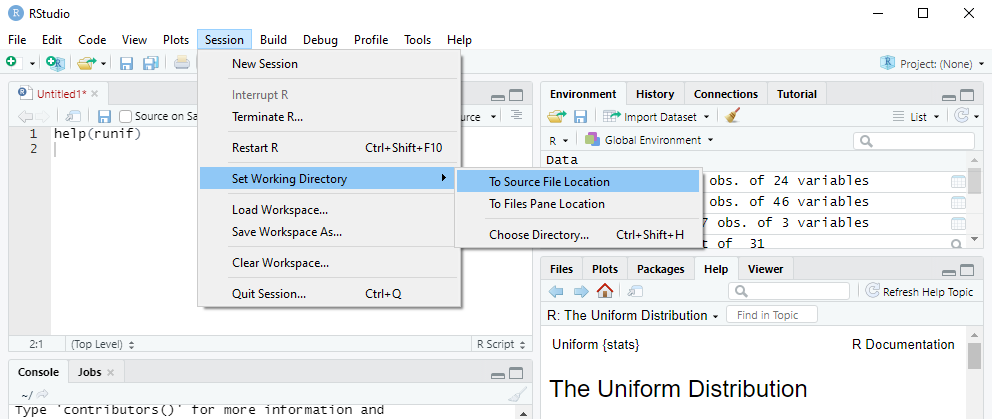
\includegraphics[width=13.78in]{img/Rstudiofig7}

\hypertarget{paquetes-o-libreruxedas}{%
\section{Paquetes o librerías}\label{paquetes-o-libreruxedas}}

Las funciones que podemos encontrar en R son limitadas. Sin embargo, R cuenta con una enorme comunidad que día a día desarrolla nuevas funciones. Estas funciones vienen empaquetadas en librerías, llamadas \textbf{packages}.
Para utilizarlas las librerías deben ser instaladas en nuestro ordenador y activadas cuando sean necesarias (no se las activa todo el tiempo para no enlentecer a la máquina)

\hypertarget{como-instalar-una-libreruxeda}{%
\subsection{¿Como instalar una librería?}\label{como-instalar-una-libreruxeda}}

Existen dos métodos para la instalación de librerías

\begin{quote}
\textbf{Recuerde}: la instalación de librerías es un proceso que sólo necesita realizar una vez, después bastará con activarla
\end{quote}

\hypertarget{instalaciuxf3n-de-libreruxeda-a-travuxe9s-de-rstudio}{%
\subsubsection{Instalación de librería a través de RStudio}\label{instalaciuxf3n-de-libreruxeda-a-travuxe9s-de-rstudio}}

Es posible instalar las librerías a ser utilizadas a través del comando de menús de RStudio para ello hay que ir al menú \texttt{Tool} y seleccionar \texttt{Install\ Packages}, se abre un cuador de diálogo en donde debemos tipear el nombre de la librería

\hypertarget{instalaciuxf3n-de-libreruxeda-a-travuxe9s-de-sintaxis}{%
\subsubsection{Instalación de librería a través de sintaxis}\label{instalaciuxf3n-de-libreruxeda-a-travuxe9s-de-sintaxis}}

Se puede utilizar la funcion \texttt{install.packages(nombre\_de\_la\_libreria)} para instalarla a través de la sintaxis

\hypertarget{como-activar-una-libreruxeda}{%
\subsection{¿Como activar una librería?}\label{como-activar-una-libreruxeda}}

La activación de una librería se realiza mediante el comando \texttt{library()}

\begin{quote}
\textbf{Importante}: Este es un proceso que debe hacerse al inicio de cada script. Seleccionamos las funciones que queremos usar y activamos las librerías que las contienen para que esten disponibles, sino no podremos usar esas funciones
\end{quote}

Bueno con todo esto en marcha vamos a empezar a trabajar\ldots{}

\hypertarget{de-la-base-de-datos-a-r}{%
\section{De la base de datos a R}\label{de-la-base-de-datos-a-r}}

\hypertarget{metodo-de-ventanas-para-subir-un-dataframe-a-r}{%
\subsection{Metodo de ventanas para subir un dataframe a R}\label{metodo-de-ventanas-para-subir-un-dataframe-a-r}}

\hypertarget{datos-desde-excel}{%
\subsubsection{Datos desde Excel}\label{datos-desde-excel}}

En la ventana Environment podemos encontrar un menu de opciones \texttt{Import\ Dataset}, si hacemos clic en esa opción se abrirá un menú que nos permitira bajar datos desde excel

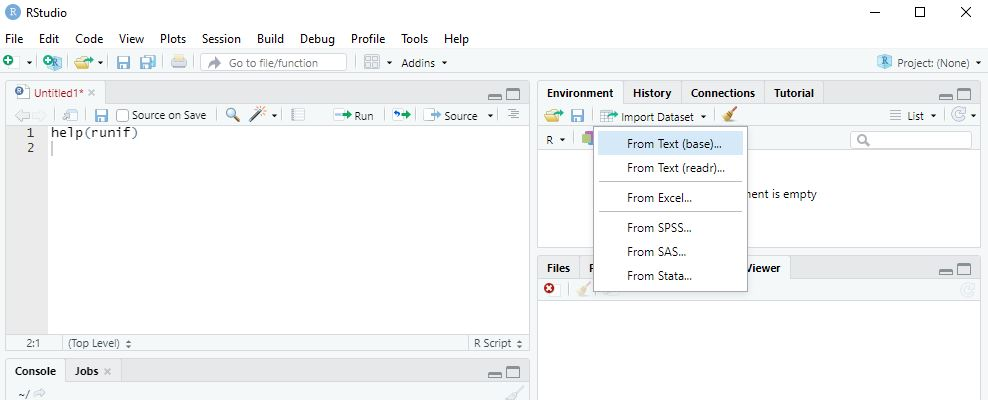
\includegraphics[width=13.72in]{img/Rstudiofig8}

Este método presenta algunas ventajas la principal es que nos muestra una previsualización de la base de datos y como se asignará la clase a cada columnas y es posible cambiar las asignación haciendo varios clics

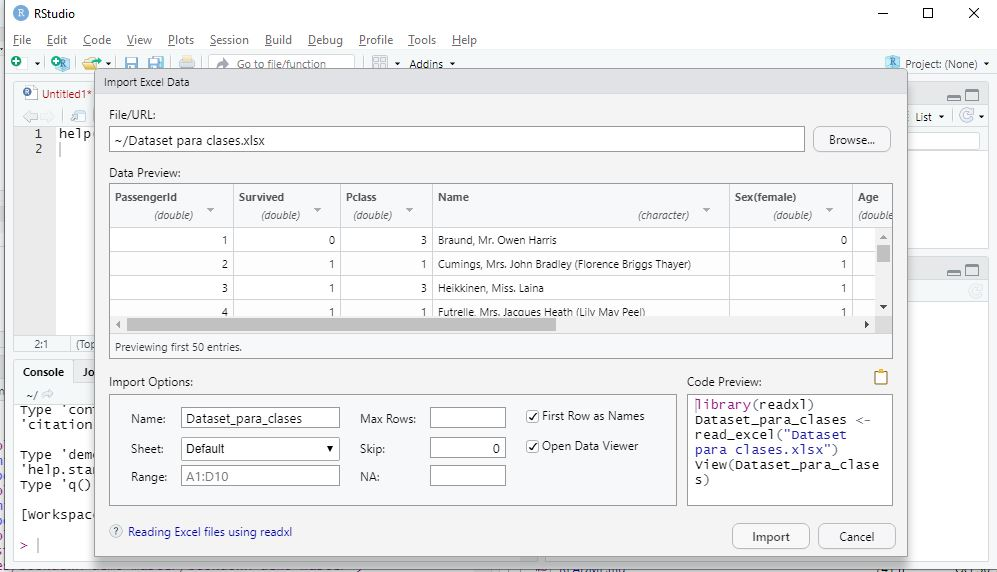
\includegraphics[width=13.85in]{img/Rstudiofig9}

Una desventaja de este método es que no hay rastro de lo que hicimos en el script y puede que no lo recordes la próxima vez que encaremos la tarea.

Una solución inteligente es copiar el cçodigo que se va autoescribiendo en la ventana \texttt{Code\ Preview}y pergarlo en nuestro script. De esa forma siempre sabemos que ocurrió

\hypertarget{datos-desde-otros-formatos}{%
\subsubsection{Datos desde otros formatos}\label{datos-desde-otros-formatos}}

El mismo método permite importar datos desde archivos de texto (CSV) o archivos de datos de SPSS (.sav) u otros programas estadísticos (SAS y Stata)

\hypertarget{cuxf3digo-para-subir-un-dataframe-a-r}{%
\subsection{Código para subir un dataframe a R}\label{cuxf3digo-para-subir-un-dataframe-a-r}}

Las alternativas mas populares es a traves de la librería readxl

Un código de ejemplo sería así

\begin{quote}
library(readxl)
data\textless-read\_excel(``nombredelarchivo.xls'')
\end{quote}

Si el archivo a utilizar no esta en la carpeta de trabajo hay que escribir la ruta hasta allí.

\hypertarget{manipulaciuxf3n-de-variables-i}{%
\section{Manipulación de variables (I)}\label{manipulaciuxf3n-de-variables-i}}

Una vez que hemos subido nuestro dataframe al programa la habilidad más importante que necesitaremos es la capacidad de manipular las variables.

En la siguiente sección aprenderemos como indicar en el lenguaje de R que necesitamos que se trabajen con ciertos datos.

El lenguaje basal de R posee un sinnumero de alternativas para manipular variables, nos limitaremos a ver las mas esenciales.

En la próxima sección seguiremos trabajando con la base de datos que creamos, si abordan esta sección sin haber leído las previas, o han limpiado su ambiente, por favor corran el siguiente código

\begin{Shaded}
\begin{Highlighting}[]
\NormalTok{numeros}\OtherTok{\textless{}{-}}\DecValTok{1}\SpecialCharTok{:}\DecValTok{10}
\NormalTok{nombres}\OtherTok{\textless{}{-}}\FunctionTok{c}\NormalTok{(}\StringTok{"Ismael"}\NormalTok{, }\StringTok{"Claudia"}\NormalTok{, }\StringTok{"Alberto"}\NormalTok{, }\StringTok{"Juan Carlos"}\NormalTok{, }\StringTok{"Laura"}\NormalTok{, }\StringTok{"José"}\NormalTok{, }\StringTok{"Luis"}\NormalTok{, }\StringTok{"Lorena"}\NormalTok{, }\StringTok{"Charly"}\NormalTok{, }\StringTok{"Fito"}\NormalTok{)}
\NormalTok{genero}\OtherTok{\textless{}{-}}\FunctionTok{c}\NormalTok{(}\StringTok{"varon"}\NormalTok{, }\StringTok{"mujer"}\NormalTok{,}\StringTok{"varon"}\NormalTok{,}\StringTok{"varon"}\NormalTok{, }\StringTok{"mujer"}\NormalTok{,}\StringTok{"varon"}\NormalTok{, }\StringTok{"varon"}\NormalTok{, }\StringTok{"mujer"}\NormalTok{,}\StringTok{"varon"}\NormalTok{,}\StringTok{"varon"}\NormalTok{)}
\NormalTok{altura\_alumnos }\OtherTok{\textless{}{-}} \FunctionTok{factor}\NormalTok{(}\FunctionTok{c}\NormalTok{(}\StringTok{"alto"}\NormalTok{, }\StringTok{"bajo"}\NormalTok{, }\StringTok{"bajo"}\NormalTok{, }\StringTok{"mediano"}\NormalTok{,}\StringTok{"bajo"}\NormalTok{, }\StringTok{"alto"}\NormalTok{, }\StringTok{"bajo"}\NormalTok{, }\StringTok{"bajo"}\NormalTok{, }\StringTok{"mediano"}\NormalTok{,}\StringTok{"bajo"}\NormalTok{),}
                       \AttributeTok{levels=}\FunctionTok{c}\NormalTok{(}\StringTok{"bajo"}\NormalTok{, }\StringTok{"mediano"}\NormalTok{, }\StringTok{"alto"}\NormalTok{))}

\FunctionTok{set.seed}\NormalTok{(}\DecValTok{123}\NormalTok{) }
\NormalTok{peso\_alumnos }\OtherTok{\textless{}{-}} \FunctionTok{runif}\NormalTok{(}\AttributeTok{n=}\DecValTok{10}\NormalTok{, }\AttributeTok{min=}\DecValTok{50}\NormalTok{, }\AttributeTok{max=}\DecValTok{100}\NormalTok{)}

\NormalTok{mi\_primera\_base}\OtherTok{\textless{}{-}}\FunctionTok{data.frame}\NormalTok{(numeros, nombres, genero, altura\_alumnos, peso\_alumnos)}
\end{Highlighting}
\end{Shaded}

\hypertarget{muxe9todos-de-selecciuxf3n-de-datos}{%
\subsection{Métodos de selección de datos}\label{muxe9todos-de-selecciuxf3n-de-datos}}

\hypertarget{el-muxe9todo-la-direcciuxf3n}{%
\subsubsection{El método \$, ``la dirección''}\label{el-muxe9todo-la-direcciuxf3n}}

Dijimos que una forma de pedirle a R que nos devuelva un objeto se basa en escribir solamente su nombre.

Si tipeamos por ejemplo el nombre de la base:

\begin{Shaded}
\begin{Highlighting}[]
\NormalTok{mi\_primera\_base}
\end{Highlighting}
\end{Shaded}

\begin{verbatim}
##    numeros     nombres genero altura_alumnos peso_alumnos
## 1        1      Ismael  varon           alto     64.37888
## 2        2     Claudia  mujer           bajo     89.41526
## 3        3     Alberto  varon           bajo     70.44885
## 4        4 Juan Carlos  varon        mediano     94.15087
## 5        5       Laura  mujer           bajo     97.02336
## 6        6        José  varon           alto     52.27782
## 7        7        Luis  varon           bajo     76.40527
## 8        8      Lorena  mujer           bajo     94.62095
## 9        9      Charly  varon        mediano     77.57175
## 10      10        Fito  varon           bajo     72.83074
\end{verbatim}

Nos devuelve la base.
El carácter \texttt{\$}: funciona como una subdirección.
Cuando ponemos el nombre de un objeto seguido del signo, R espera el nombre de otro objeto contenido dentro de el (como si fuera una dirección, antes del \texttt{\$} escribimos el numero de la calle, y después el departamento).

Miremos este ejemplo

\begin{Shaded}
\begin{Highlighting}[]
\NormalTok{mi\_primera\_base}\SpecialCharTok{$}\NormalTok{genero}
\end{Highlighting}
\end{Shaded}

\begin{verbatim}
##  [1] "varon" "mujer" "varon" "varon" "mujer" "varon" "varon" "mujer" "varon"
## [10] "varon"
\end{verbatim}

como vemos, R entendió que le pedíamos sólo \emph{genero}, que está contenido en \emph{mi\_primera\_base}.
Este método (de dirección), es muy útil porque puede que este trabajando con dos bases en simultáneo con columnas del mismo nombre (por ejemplo genero). Entonces existen dos objetos \emph{genero} pero únicos en su dirección.

El resultante de este método es un objeto, y podemos manipularlo.

Veamos un ejemplo de la vida real.

Queremos calcular la media del peso de los alumnos, la sintaxis sería más o menos así.

\begin{Shaded}
\begin{Highlighting}[]
\FunctionTok{mean}\NormalTok{(mi\_primera\_base}\SpecialCharTok{$}\NormalTok{peso\_alumnos)}
\end{Highlighting}
\end{Shaded}

\begin{verbatim}
## [1] 78.91238
\end{verbatim}

Como vemos la funcion \texttt{mean()} funcionó absolutamente igual que si le hubiéramos pedido que calculara la media del objeto \emph{peso\_alumnos}, sin que pertenezca a un dataframe

Este método de dirección es útil también para crear nuevas variables dentro del dataframe (siempre y cuando tenga el mismo \emph{largo} que las otras columnas).

Probemos creando al azar una columna de edad. Para ello vamos a seguir los siguientes pasos:
1. Vamos a usar la función \texttt{runif()}, para crear numeros aleatorios, entre 10 y 30
2. le vamos a aplicar la función \texttt{round()} para que redondee esos números a enteros
3. Y vamos a escribir ese resultado en una columna \emph{edad} directamente en el dataframe.
4. Después vamos a previsualizar los primeros 3 elementos del dataframe para ver que pasó.

Veamos como:

\begin{Shaded}
\begin{Highlighting}[]
\NormalTok{mi\_primera\_base}\SpecialCharTok{$}\NormalTok{edad }\OtherTok{\textless{}{-}} \FunctionTok{round}\NormalTok{(}\FunctionTok{runif}\NormalTok{(}\AttributeTok{n=}\DecValTok{10}\NormalTok{, }\AttributeTok{min=}\DecValTok{10}\NormalTok{, }\AttributeTok{max=}\DecValTok{30}\NormalTok{))}

\FunctionTok{head}\NormalTok{(mi\_primera\_base)}
\end{Highlighting}
\end{Shaded}

\begin{verbatim}
##   numeros     nombres genero altura_alumnos peso_alumnos edad
## 1       1      Ismael  varon           alto     64.37888   29
## 2       2     Claudia  mujer           bajo     89.41526   19
## 3       3     Alberto  varon           bajo     70.44885   24
## 4       4 Juan Carlos  varon        mediano     94.15087   21
## 5       5       Laura  mujer           bajo     97.02336   12
## 6       6        José  varon           alto     52.27782   28
\end{verbatim}

Hemos aprendido dos cosas, muchas funciones se pueden \textbf{anidar} simplemente con el uso de paréntesis como si se tratara de una operación matemática.
La segunda, la màs importante: \_ podemos utilizar el método de la direccion de \$ para crear nuevas columnas\_

Como funciona esto, si a R le damos una dirección dentro de nuestra base que no existe simplemente la crea.

\begin{quote}
Cuidado, si asignamos a una dirección existente nuevos datos, va a escribir estos en la dirección indicada borrando los anteriores
\end{quote}

\hypertarget{ejercicios-1}{%
\paragraph{\texorpdfstring{ Ejercicios}{ Ejercicios}}\label{ejercicios-1}}

Realicemos ahora algunas transformaciones de variables utilizando este método.

\begin{enumerate}
\def\labelenumi{\arabic{enumi}.}
\tightlist
\item
  Supongamos que en lugar de la edad de los sujetos, necesitamos el año en que nacieron. Para ello vamos a crear una nueva variable \emph{anio\_nacimiento} y le vamos a asignar la transformación de la edad al año.
\end{enumerate}

\begin{Shaded}
\begin{Highlighting}[]
\NormalTok{mi\_primera\_base}\SpecialCharTok{$}\NormalTok{anio\_nacimiento }\OtherTok{\textless{}{-}} \DecValTok{2021}\SpecialCharTok{{-}}\NormalTok{mi\_primera\_base}\SpecialCharTok{$}\NormalTok{edad}

\FunctionTok{head}\NormalTok{(mi\_primera\_base)}
\end{Highlighting}
\end{Shaded}

\begin{verbatim}
##   numeros     nombres genero altura_alumnos peso_alumnos edad anio_nacimiento
## 1       1      Ismael  varon           alto     64.37888   29            1992
## 2       2     Claudia  mujer           bajo     89.41526   19            2002
## 3       3     Alberto  varon           bajo     70.44885   24            1997
## 4       4 Juan Carlos  varon        mediano     94.15087   21            2000
## 5       5       Laura  mujer           bajo     97.02336   12            2009
## 6       6        José  varon           alto     52.27782   28            1993
\end{verbatim}

Como ven resolvimos el problema de una manera sencilla con las operaciones que vimos.
Le pedimos a R que a 2021 le reste la edad de cada sujeto y los resultados los vaya guardando en la nueva variable.
Una vez que nos acostumbramos a la sintaxis es muy sencillo transformar variables con este método.

Practiquemos un poco más:

\begin{enumerate}
\def\labelenumi{\arabic{enumi}.}
\setcounter{enumi}{1}
\tightlist
\item
  Tranformemos el peso de los alumnos en libras.
\end{enumerate}

\begin{Shaded}
\begin{Highlighting}[]
\NormalTok{mi\_primera\_base}\SpecialCharTok{$}\NormalTok{peso\_enlbs }\OtherTok{\textless{}{-}}\NormalTok{ mi\_primera\_base}\SpecialCharTok{$}\NormalTok{peso\_alumnos}\SpecialCharTok{*}\FloatTok{2.20462262185}

\FunctionTok{head}\NormalTok{(mi\_primera\_base)}
\end{Highlighting}
\end{Shaded}

\begin{verbatim}
##   numeros     nombres genero altura_alumnos peso_alumnos edad anio_nacimiento
## 1       1      Ismael  varon           alto     64.37888   29            1992
## 2       2     Claudia  mujer           bajo     89.41526   19            2002
## 3       3     Alberto  varon           bajo     70.44885   24            1997
## 4       4 Juan Carlos  varon        mediano     94.15087   21            2000
## 5       5       Laura  mujer           bajo     97.02336   12            2009
## 6       6        José  varon           alto     52.27782   28            1993
##   peso_enlbs
## 1   141.9311
## 2   197.1269
## 3   155.3131
## 4   207.5671
## 5   213.8999
## 6   115.2529
\end{verbatim}

\begin{enumerate}
\def\labelenumi{\arabic{enumi}.}
\setcounter{enumi}{2}
\tightlist
\item
  Imaginen que quieren dicotomizar la variable altura, y dividirla en los que son altos y los que no. Para ello podemos crear una variable a través de una función logica. Vemos que sencillo es:
\end{enumerate}

\begin{Shaded}
\begin{Highlighting}[]
\NormalTok{mi\_primera\_base}\SpecialCharTok{$}\NormalTok{alto\_y\_n }\OtherTok{\textless{}{-}}\NormalTok{ mi\_primera\_base}\SpecialCharTok{$}\NormalTok{altura\_alumnos}\SpecialCharTok{==}\StringTok{"alto"}

\FunctionTok{head}\NormalTok{(mi\_primera\_base)}
\end{Highlighting}
\end{Shaded}

\begin{verbatim}
##   numeros     nombres genero altura_alumnos peso_alumnos edad anio_nacimiento
## 1       1      Ismael  varon           alto     64.37888   29            1992
## 2       2     Claudia  mujer           bajo     89.41526   19            2002
## 3       3     Alberto  varon           bajo     70.44885   24            1997
## 4       4 Juan Carlos  varon        mediano     94.15087   21            2000
## 5       5       Laura  mujer           bajo     97.02336   12            2009
## 6       6        José  varon           alto     52.27782   28            1993
##   peso_enlbs alto_y_n
## 1   141.9311     TRUE
## 2   197.1269    FALSE
## 3   155.3131    FALSE
## 4   207.5671    FALSE
## 5   213.8999    FALSE
## 6   115.2529     TRUE
\end{verbatim}

Creamos una variable lógica (que tambien funciona como una dictomica 0/1, recuerdan?)

\hypertarget{el-muxe9todo-phil-collins}{%
\subsubsection{El método ``Phil Collins''}\label{el-muxe9todo-phil-collins}}

vamos a ver otro método de manipular datos y variables, este método es ligeramente màs flexible que el anterior.

¿Recuerdan la siguiente notación?:

\texttt{genero\ \textbar{}\ chr{[}1:10{]}}

Esta era la forma de R de decirnos que se trataba de un objeto de 1 fila y 10 columnas, ¿no?.

Recordemos que siempre van primero las filas y después las columnas (\textbf{mnemotecnia Phil Collins})

Con el mismo criterio podemos usar los corchetes como una dirección!!

Si una columna tiene 10 filas (o sea \texttt{{[}1:10{]}}), el contenido de esas 10 filas està etiquetado ( de arriba abajo) con valores del 1 al 10. A estas etiquetas las llamamos \textbf{índices}.

Cada valor de nuestro dataframe tiene entonces un ìndice propio de columna y de fila (una direcciòn para cada valor!!!)

De esta forma

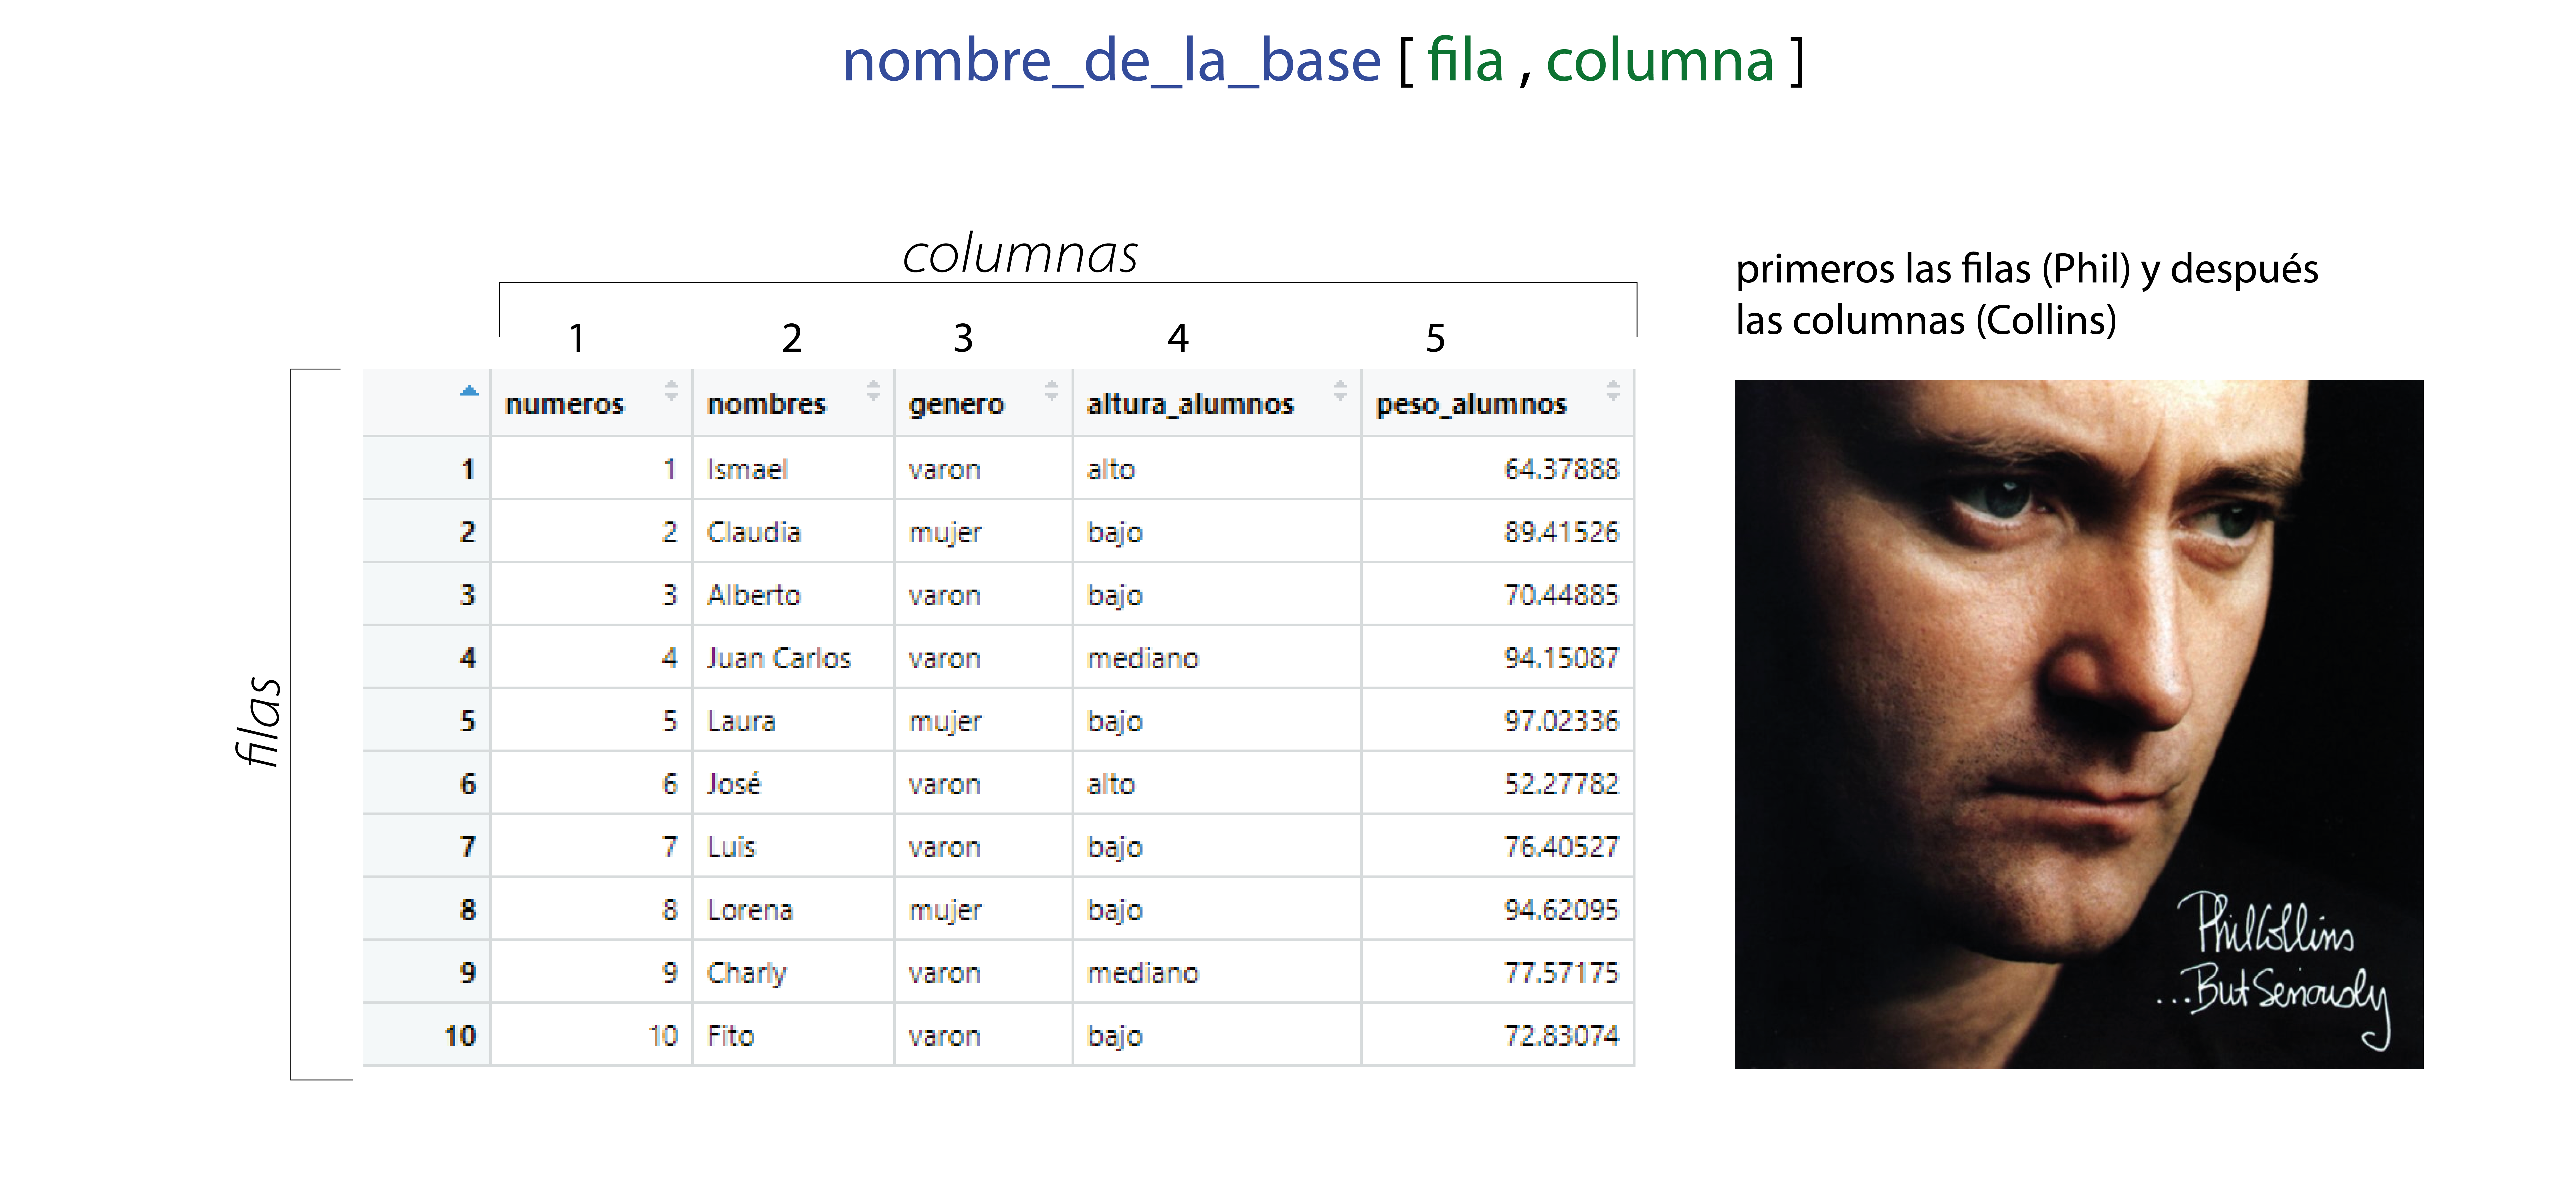
\includegraphics{img/philcollins.png}

Este mètodo nos permite seleccionar valores particulares.
Veamos por ejemplo si quisieramos saber el nombre del tercer alumno de la base:

\begin{Shaded}
\begin{Highlighting}[]
\NormalTok{mi\_primera\_base[}\DecValTok{3}\NormalTok{,}\DecValTok{2}\NormalTok{]}
\end{Highlighting}
\end{Shaded}

\begin{verbatim}
## [1] "Alberto"
\end{verbatim}

Como leemos esto: le pedimos a R que dentro de la base \emph{mi\_primera\_base} nos devuelva el valor en la posición fila 3 y columna 2 (la de los nombres)

Por su simpleza este método es muy flexible.

\begin{quote}
\textbf{Aclaración}: Cuando dejemos uno de estos dos parámetros vacíos, R va a interpretar que le pedimos \textbf{todos!}
\end{quote}

Veamos ahora si necesitaramos \emph{toda} la columna nombres escribiríamos lo siguiente:

\begin{Shaded}
\begin{Highlighting}[]
\NormalTok{mi\_primera\_base[,}\DecValTok{2}\NormalTok{]}
\end{Highlighting}
\end{Shaded}

\begin{verbatim}
##  [1] "Ismael"      "Claudia"     "Alberto"     "Juan Carlos" "Laura"      
##  [6] "José"        "Luis"        "Lorena"      "Charly"      "Fito"
\end{verbatim}

Tenemos los 10 registros de la columna nombres.

Si quisieramos los 5 primeros, por ejemplo

\begin{Shaded}
\begin{Highlighting}[]
\NormalTok{mi\_primera\_base[}\DecValTok{1}\SpecialCharTok{:}\DecValTok{5}\NormalTok{,}\DecValTok{2}\NormalTok{]}
\end{Highlighting}
\end{Shaded}

\begin{verbatim}
## [1] "Ismael"      "Claudia"     "Alberto"     "Juan Carlos" "Laura"
\end{verbatim}

Recuerden que utilizabamos \texttt{:} para indicar, todos los valores de 1 a 5.

Este método funciona igual que el mètodo \texttt{\$} a la hora de aplicar funciones.
Veamos este ejemplo para calcular la media del peso (columna 5)

\begin{Shaded}
\begin{Highlighting}[]
\FunctionTok{mean}\NormalTok{(mi\_primera\_base[,}\DecValTok{5}\NormalTok{])}
\end{Highlighting}
\end{Shaded}

\begin{verbatim}
## [1] 78.91238
\end{verbatim}

Si subimos en el texto vemos que el resultado es el mismo con ambos métodos. Si leemos el código en voz alta sería algo así: ``Calcular la media de todas las filas de la columna 5 de la base \emph{mi\_primera\_base}''

\hypertarget{manipulaciuxf3n-de-variables-ii}{%
\chapter{Manipulación de variables (II)}\label{manipulaciuxf3n-de-variables-ii}}

En esta sección vamos a ver fundamentos sencillos de manipulación de datos mediante la gramática del tidiverse (paciencia que suena rarísimo, pero es una pavada).
Para eso vamos a utilizar dos paquetes: dplyr (que contiene las funciones para manipular los datos) y gapminder que es un paquete con bases de datos de PBI mundiales, vamos a activarlos ( e instalarlos si no los tienen)

\begin{Shaded}
\begin{Highlighting}[]
\DocumentationTok{\#\# estos son los comandos para instalar }
\CommentTok{\#(también pueden hacerlo desde tools{-}\textgreater{} install package)}
\CommentTok{\#recuerden remover los "\#" para que la línea se ejecute }


\CommentTok{\# install.packages("gapminder")}
\CommentTok{\# install.packages("dplyr") }


\DocumentationTok{\#\#y estos los comandos para activarlos}

\FunctionTok{library}\NormalTok{(}\StringTok{"gapminder"}\NormalTok{)}
\FunctionTok{library}\NormalTok{(}\StringTok{"dplyr"}\NormalTok{)}
\end{Highlighting}
\end{Shaded}

\begin{verbatim}
## 
## Attaching package: 'dplyr'
\end{verbatim}

\begin{verbatim}
## The following objects are masked from 'package:stats':
## 
##     filter, lag
\end{verbatim}

\begin{verbatim}
## The following objects are masked from 'package:base':
## 
##     intersect, setdiff, setequal, union
\end{verbatim}

Vamos a asignar nuestros datos a un objeto base local así los podemos visualizar en el ambiente

\begin{Shaded}
\begin{Highlighting}[]
\NormalTok{data}\OtherTok{\textless{}{-}}\NormalTok{gapminder}
\end{Highlighting}
\end{Shaded}

Listo con los preliminares, ahora tenemos una base de datos en nuestro ambiente con 6 variables y 1704 observaciones (no es así? :-\textless, revisen la sintaxis)

\hypertarget{piping-y-paquete-dplyr}{%
\section{Piping y paquete dplyr}\label{piping-y-paquete-dplyr}}

En la primera sección vimos cuan importante es el operador de asignación \textbf{-\textgreater{}}. Bueno ahora veremos uno más potente aún, la pipa o \textbf{pipe}. Este operador se escribe de la siguiente forma \%\textgreater\%. fue introducido por el paquete dplyr (el que vamos a usar aquí), pero su dinàmica es tan buena que ha sido replicado por muchos paquetes para ordenar datos (el conocido como tidiverse)


\includegraphics[width=90.4in]{img/memedrake}

Es uno de los operadores más utilizados por su versatilidad. Este signo se escribe antecediendo una función de dplyr. Veamos como lo lee R.

Una sintaxis de dplyr seria por ejemplo asi

\begin{quote}
data \%\textgreater\% filter(year==1992)
\end{quote}

Esto se lee así, a la base data \textbf{apliquemosle} la función filter (y la función filter en este caso se lee, filtrar todos los registros en donde el año es 1992)

Una de las maravillas de este operador es que puede concatenarse, y eso nos permite aplicar varias funciones en orden como un flujo de trabajos o \textbf{piping}. Veamos como.

\begin{quote}
data \%\textgreater\% filter(year==1992) \%\textgreater\% filter(continent==``Asia'')
\end{quote}

Esto se lee así, a la base data \textbf{apliquemosle} la función filter (y filtremos sólo los registros en donde el año es 1992); a lo que quedó, \textbf{apliquemosle} la función filter (y filtremos sólo los registros del continente asiático)

Si corren estas lineas veran que el resultado se muestra como una base de datos en la \emph{consola}, es probable que con estos datos querramos trabajar a continuación, para que eso pase debemos convertirlo en un \emph{objeto} del ambiente, con nuestro viejo amigo el operador \emph{-\textgreater{}}, algo así:

\begin{quote}
data\_filtrada \textless- data \%\textgreater\% filter(year==1992) \%\textgreater\% filter(continent==``Asia'')
\end{quote}

Esto lo leeríamos así: en el objeto \emph{datafiltrada} \textbf{asignemos} el resultado de las operaciones de agarrar la base data \textbf{aplicarle} la función filter (y filtremos sólo los registros en donde el año es 1992); y a lo que quedó, \textbf{aplicarle} la función filter (y filtremos sólo los registros del continente asiático).

Una vez que aprendimos del piping vamos a aprender las funciones de dplyr màs útiles.

\hypertarget{funciones-dplyr}{%
\section{Funciones dplyr}\label{funciones-dplyr}}

Dplyr tiene muchísimas funciones, en esta seccion veremos sólo algunas: la función \texttt{filter()} o filtrado, que nos permite seleccionar todas las \emph{filas} que cumplan con una condición, la función \texttt{select()} que nos permite \_seleccionar sólo algunas columnas del dataset. La función \texttt{arrange()} que sirve para ordenar los datos en función del agun criterio y la función \texttt{mutate()} para crear nuevas variables.

\begin{quote}
\textbf{Aclaración}: Probablemente llegado a este punto se plantearán que ya concen métodos para crear una nueva variable (con el método de \$) o incluso podemos usar nuestro método Phil Colins para filtrar por condiciones, es cierto.

Una cosa interesante de R, es que hay varias formas de decir lo mismo (como en un lenguaje, recuerdan), e incluso podemos mezclar estilos (hacer un piping y usar cosas del método phil colins por ejemplo)
\end{quote}

Zarpemos a la aventura

\hypertarget{funciuxf3n-filter}{%
\subsection{Función filter()}\label{funciuxf3n-filter}}

Esta función tiene la tarea de seleccionar las observaciones (filas) que cumplen las condiciones que nos interesan.
Tiene una sintaxis muy sencilla simplemente ponemos la variable y la condición (recuerden que el nombre del dataframe se lo dimos en el piping), ya vimos ejemplos de como usarla, pero nunca vienen mal otros:

\begin{enumerate}
\def\labelenumi{\arabic{enumi}.}
\tightlist
\item
  Quiero obtener un dataset con solo los datos de Argentina, y lo quiero llamar PBIArg, deberíamos escribir algo así.
\end{enumerate}

\begin{Shaded}
\begin{Highlighting}[]
\NormalTok{ PBIArg }\OtherTok{\textless{}{-}}\NormalTok{ data }\SpecialCharTok{\%\textgreater{}\%} \FunctionTok{filter}\NormalTok{ (country }\SpecialCharTok{==} \StringTok{"Argentina"}\NormalTok{)}
\end{Highlighting}
\end{Shaded}

Se animan a hacer algunas funciones clásicas ahora?

Calculemos el PBI percapita promedio en todos estos años de la base.

\begin{Shaded}
\begin{Highlighting}[]
\FunctionTok{mean}\NormalTok{(PBIArg}\SpecialCharTok{$}\NormalTok{gdpPercap)}
\end{Highlighting}
\end{Shaded}

\begin{verbatim}
## [1] 8955.554
\end{verbatim}

¿Se animan algo más complejo?, como contestarían la pregunta: ¿Cuál fue el PBI Argentino en 1982?, bueno podemos resolverlo de dos maneras ahora que tenemos el objeto PBIArg

Manera 1:

\begin{Shaded}
\begin{Highlighting}[]
\NormalTok{PBIArg }\SpecialCharTok{\%\textgreater{}\%} \FunctionTok{filter}\NormalTok{ (year }\SpecialCharTok{==}\DecValTok{1982}\NormalTok{)}
\end{Highlighting}
\end{Shaded}

\begin{verbatim}
## # A tibble: 1 x 6
##   country   continent  year lifeExp      pop gdpPercap
##   <fct>     <fct>     <int>   <dbl>    <int>     <dbl>
## 1 Argentina Americas   1982    69.9 29341374     8998.
\end{verbatim}

Manera 2:

\begin{Shaded}
\begin{Highlighting}[]
\NormalTok{data }\SpecialCharTok{\%\textgreater{}\%} \FunctionTok{filter}\NormalTok{(country}\SpecialCharTok{==}\StringTok{"Argentina"}\NormalTok{) }\SpecialCharTok{\%\textgreater{}\%} \FunctionTok{filter}\NormalTok{(year}\SpecialCharTok{==}\DecValTok{1982}\NormalTok{)}
\end{Highlighting}
\end{Shaded}

\begin{verbatim}
## # A tibble: 1 x 6
##   country   continent  year lifeExp      pop gdpPercap
##   <fct>     <fct>     <int>   <dbl>    <int>     <dbl>
## 1 Argentina Americas   1982    69.9 29341374     8998.
\end{verbatim}

El resultado fue el mismo! Hagan el ejercicio de leer el \emph{piping} en voz alta. ¿Cual opción les parece mejor?, si bien no hay una sóla respuesta a esto, la manera 2 es muy útil si sólo queremos un dato de Argentina porque no crea una objeto intermedio (en este caso, PBIArg) Ahora no parece un problema pero cuando trabajen más de 15 minutos van a darse cuenta que su ambiente se llena de \emph{objetos basura} si no somos cuidadosos y complica mucho el trabajo.

Resumiendo la función filter() haría algo así.

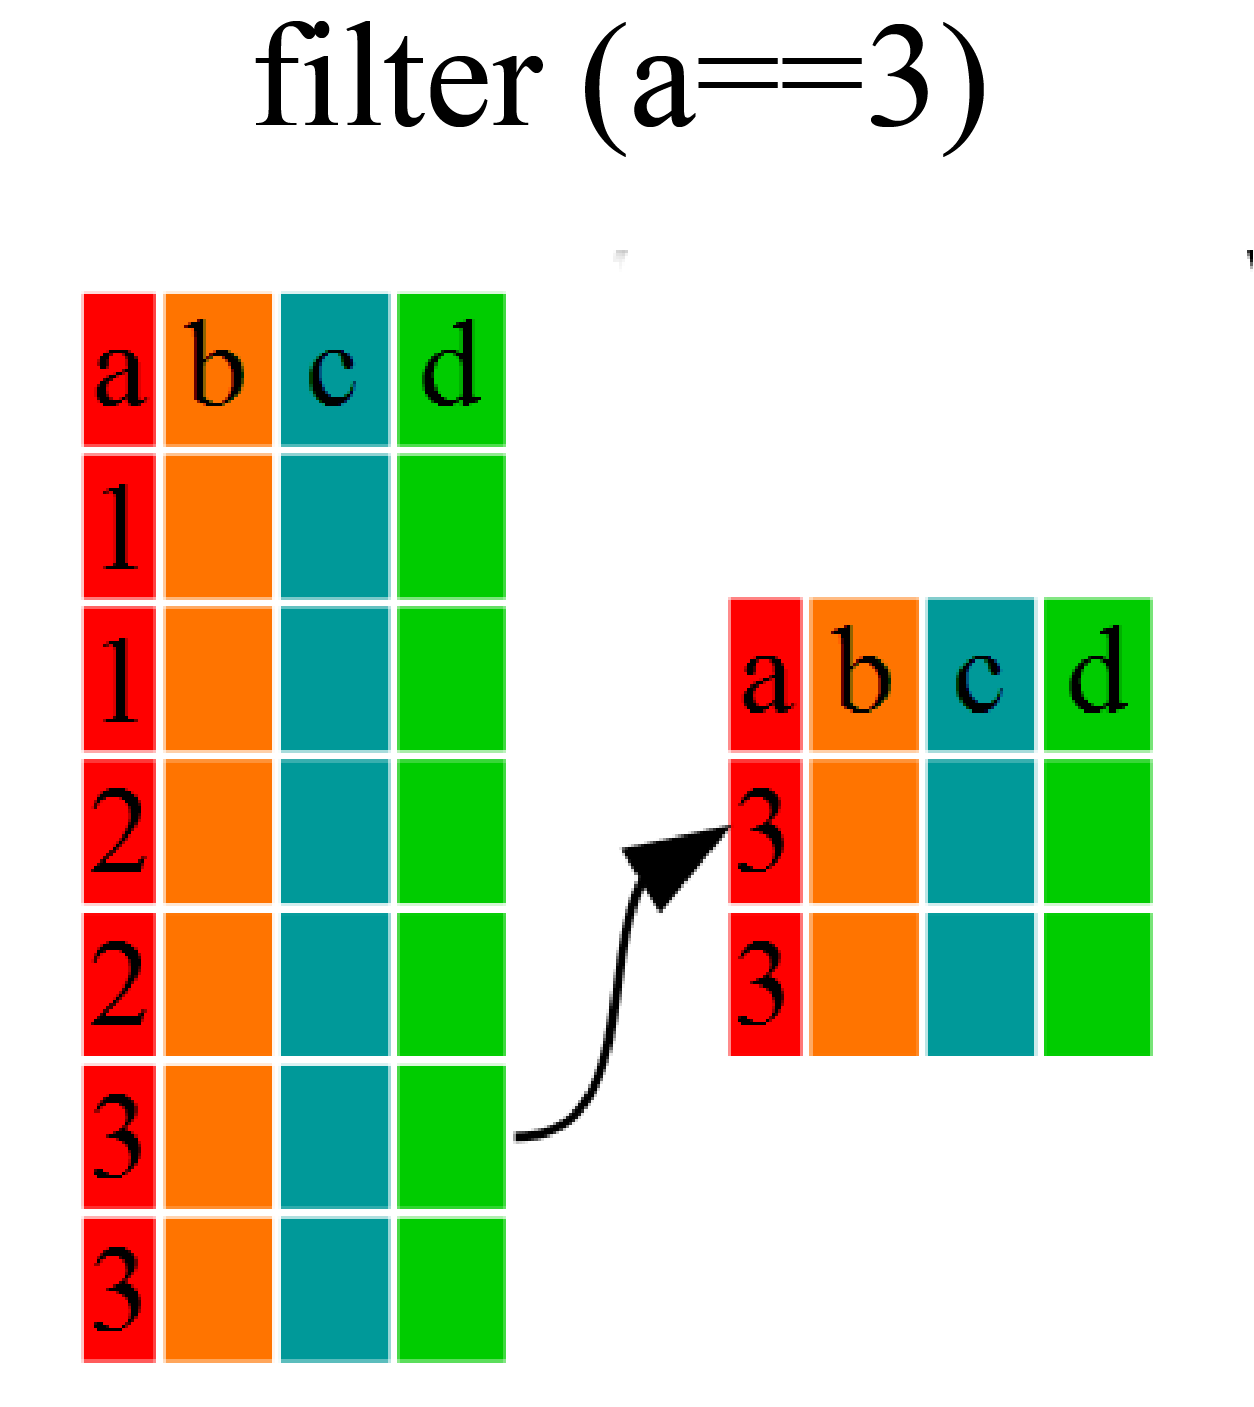
\includegraphics[width=17.42in]{img/filter}

\hypertarget{funciuxf3n-select}{%
\section{Función select()}\label{funciuxf3n-select}}

La función select sirve para seleccionar columnas completas, ¿para que puede servir algo así?.

Siganme un poco con el ejemplo:

Primero vamos a cargar una base que esta en R que se llama iris (que son medidas de ancho y largo del pétalo y el sépalo de florecitas de tres variedades distintas encontradas en el mismo campo medidas por un sr Ronald Fisher - que cuando no medía flores estaba revolucionando la estadística-), carguemos la base y veamos que tipos de variables son:

\begin{Shaded}
\begin{Highlighting}[]
\NormalTok{flores}\OtherTok{\textless{}{-}}\NormalTok{iris}

\FunctionTok{str}\NormalTok{(flores)}
\end{Highlighting}
\end{Shaded}

\begin{verbatim}
## 'data.frame':    150 obs. of  5 variables:
##  $ Sepal.Length: num  5.1 4.9 4.7 4.6 5 5.4 4.6 5 4.4 4.9 ...
##  $ Sepal.Width : num  3.5 3 3.2 3.1 3.6 3.9 3.4 3.4 2.9 3.1 ...
##  $ Petal.Length: num  1.4 1.4 1.3 1.5 1.4 1.7 1.4 1.5 1.4 1.5 ...
##  $ Petal.Width : num  0.2 0.2 0.2 0.2 0.2 0.4 0.3 0.2 0.2 0.1 ...
##  $ Species     : Factor w/ 3 levels "setosa","versicolor",..: 1 1 1 1 1 1 1 1 1 1 ...
\end{verbatim}

Bueno si todo les salió bien (como a mí) van a tener que hayt 4 variables numéricas (los anchos y largos) y un factor (una categórica que es la variedad de la flor)

Bueno hete aquí el problemita que que entre los defectos de Ronald Fisher (además de un poquito de racismo) estaba el ser inglés y tomó todas estas medias en pulgadas. nosotros investigadores del nuevo milenio queremos pasar esto al sistema internacional (con medidas más logicas que el tamaño del pulgar de un rey muerto)

¿Cómo hacemos eso? Bueno ya vimos algunas soluciones en el capítulo anterior. Las voy a ejecutar a modo de repaso

\begin{Shaded}
\begin{Highlighting}[]
\CommentTok{\# creo dentro de flor nuevas variables ajustadas}

\NormalTok{flores}\SpecialCharTok{$}\NormalTok{Sepal.Lengthcm}\OtherTok{\textless{}{-}}\NormalTok{flores}\SpecialCharTok{$}\NormalTok{Sepal.Length}\SpecialCharTok{*}\FloatTok{2.54} \CommentTok{\#multiplicamos por 2.54 cada valor para pasarlo a cm }
\NormalTok{flores}\SpecialCharTok{$}\NormalTok{Sepal.Widthcm}\OtherTok{\textless{}{-}}\NormalTok{flores}\SpecialCharTok{$}\NormalTok{Sepal.Width}\SpecialCharTok{*}\FloatTok{2.54}
\NormalTok{flores}\SpecialCharTok{$}\NormalTok{Petal.Lengthcm}\OtherTok{\textless{}{-}}\NormalTok{flores}\SpecialCharTok{$}\NormalTok{Petal.Length}\SpecialCharTok{*}\FloatTok{2.54}
\NormalTok{flores}\SpecialCharTok{$}\NormalTok{Petal.Widthcm}\OtherTok{\textless{}{-}}\NormalTok{flores}\SpecialCharTok{$}\NormalTok{Petal.Width}\SpecialCharTok{*}\FloatTok{2.54}

\FunctionTok{str}\NormalTok{(flores)}
\end{Highlighting}
\end{Shaded}

\begin{verbatim}
## 'data.frame':    150 obs. of  9 variables:
##  $ Sepal.Length  : num  5.1 4.9 4.7 4.6 5 5.4 4.6 5 4.4 4.9 ...
##  $ Sepal.Width   : num  3.5 3 3.2 3.1 3.6 3.9 3.4 3.4 2.9 3.1 ...
##  $ Petal.Length  : num  1.4 1.4 1.3 1.5 1.4 1.7 1.4 1.5 1.4 1.5 ...
##  $ Petal.Width   : num  0.2 0.2 0.2 0.2 0.2 0.4 0.3 0.2 0.2 0.1 ...
##  $ Species       : Factor w/ 3 levels "setosa","versicolor",..: 1 1 1 1 1 1 1 1 1 1 ...
##  $ Sepal.Lengthcm: num  13 12.4 11.9 11.7 12.7 ...
##  $ Sepal.Widthcm : num  8.89 7.62 8.13 7.87 9.14 ...
##  $ Petal.Lengthcm: num  3.56 3.56 3.3 3.81 3.56 ...
##  $ Petal.Widthcm : num  0.508 0.508 0.508 0.508 0.508 ...
\end{verbatim}

Perfecto, este método funciona. Pero, pero, pero: tuvimos que escribir una línea super engorrosa por cada variable (en este caso eran 4, pero si son no sé, 60, se pasarían toda la tarde), tiene que haber una forma de simplificar esto.

¿Que pasa si multiplicamos toooda la base *2.54?

\begin{Shaded}
\begin{Highlighting}[]
\FunctionTok{head}\NormalTok{(flores}\SpecialCharTok{*}\FloatTok{2.54}\NormalTok{)}
\end{Highlighting}
\end{Shaded}

\begin{verbatim}
## Warning in Ops.factor(left, right): '*' not meaningful for factors
\end{verbatim}

\begin{verbatim}
##   Sepal.Length Sepal.Width Petal.Length Petal.Width Species Sepal.Lengthcm
## 1       12.954       8.890        3.556       0.508      NA       32.90316
## 2       12.446       7.620        3.556       0.508      NA       31.61284
## 3       11.938       8.128        3.302       0.508      NA       30.32252
## 4       11.684       7.874        3.810       0.508      NA       29.67736
## 5       12.700       9.144        3.556       0.508      NA       32.25800
## 6       13.716       9.906        4.318       1.016      NA       34.83864
##   Sepal.Widthcm Petal.Lengthcm Petal.Widthcm
## 1      22.58060        9.03224       1.29032
## 2      19.35480        9.03224       1.29032
## 3      20.64512        8.38708       1.29032
## 4      19.99996        9.67740       1.29032
## 5      23.22576        9.03224       1.29032
## 6      25.16124       10.96772       2.58064
\end{verbatim}

\begin{Shaded}
\begin{Highlighting}[]
\CommentTok{\#acá anide la multiplicación dentro de la función head() para que sólo muestre el pimer pedacito de la tabla}
\end{Highlighting}
\end{Shaded}

¿Que pasó con la variables \emph{Species}? Bueno le aplicó la multiplicación a una palabra, la multiplicación por una palabra no existe o sea que me borró los datos.
Nosotros queríamos comparar las diferencias entre esas plantas así que ahora, estamos fritos! Tenemos los cm pero perdimos una variable.

Acá entrá (y si hizo esperar), la función \texttt{select()}

Dijimos que esta función sirve para quedarno con sólo algunas columnas (como hace fiulter con las filas)

Miren como lo haríamos

\begin{Shaded}
\begin{Highlighting}[]
\NormalTok{medidas\_Flores}\OtherTok{\textless{}{-}}\NormalTok{flores }\SpecialCharTok{\%\textgreater{}\%} \FunctionTok{select}\NormalTok{(Sepal.Length}\SpecialCharTok{:}\NormalTok{Petal.Width)}

\FunctionTok{head}\NormalTok{(medidas\_Flores)}
\end{Highlighting}
\end{Shaded}

\begin{verbatim}
##   Sepal.Length Sepal.Width Petal.Length Petal.Width
## 1          5.1         3.5          1.4         0.2
## 2          4.9         3.0          1.4         0.2
## 3          4.7         3.2          1.3         0.2
## 4          4.6         3.1          1.5         0.2
## 5          5.0         3.6          1.4         0.2
## 6          5.4         3.9          1.7         0.4
\end{verbatim}

Aquí tenemos las 4 variables

ahora podemos transformarlas:

\begin{Shaded}
\begin{Highlighting}[]
\NormalTok{medidas\_Flores}\OtherTok{\textless{}{-}}\NormalTok{medidas\_Flores}\SpecialCharTok{*}\FloatTok{2.54}

\FunctionTok{head}\NormalTok{(medidas\_Flores)}
\end{Highlighting}
\end{Shaded}

\begin{verbatim}
##   Sepal.Length Sepal.Width Petal.Length Petal.Width
## 1       12.954       8.890        3.556       0.508
## 2       12.446       7.620        3.556       0.508
## 3       11.938       8.128        3.302       0.508
## 4       11.684       7.874        3.810       0.508
## 5       12.700       9.144        3.556       0.508
## 6       13.716       9.906        4.318       1.016
\end{verbatim}

y podemos pegarle la categoría que nos quedó colgada

\begin{Shaded}
\begin{Highlighting}[]
\NormalTok{medidas\_Flores}\SpecialCharTok{$}\NormalTok{especie}\OtherTok{\textless{}{-}}\NormalTok{flores}\SpecialCharTok{$}\NormalTok{Species}

\FunctionTok{head}\NormalTok{(medidas\_Flores)}
\end{Highlighting}
\end{Shaded}

\begin{verbatim}
##   Sepal.Length Sepal.Width Petal.Length Petal.Width especie
## 1       12.954       8.890        3.556       0.508  setosa
## 2       12.446       7.620        3.556       0.508  setosa
## 3       11.938       8.128        3.302       0.508  setosa
## 4       11.684       7.874        3.810       0.508  setosa
## 5       12.700       9.144        3.556       0.508  setosa
## 6       13.716       9.906        4.318       1.016  setosa
\end{verbatim}

Ahora sí ya podemos trabajar con la base de Fisher en cm y sin perder datos

Pero momentito, esta función no aporta nada nuevo. Podemos hacer esto mismo con la sintaxis que aprendimos en el capítulo anterior (si con el método Phil Colins).

Vamos a hacer el intento

\begin{Shaded}
\begin{Highlighting}[]
\FunctionTok{rm}\NormalTok{(medidas\_Flores) }\CommentTok{\# esta función borra la base, así no creamos miles de objeto}


\NormalTok{medidas\_Flores}\OtherTok{\textless{}{-}}\NormalTok{flores[,}\DecValTok{1}\SpecialCharTok{:}\DecValTok{4}\NormalTok{] }\CommentTok{\#le pedi todas las filas de la columna 1 a la 4 (que son las medidas)}

\NormalTok{medidas\_Flores}\OtherTok{\textless{}{-}}\NormalTok{medidas\_Flores}\SpecialCharTok{*}\FloatTok{2.54} \CommentTok{\#las transformo}

\NormalTok{medidas\_Flores}\SpecialCharTok{$}\NormalTok{especie}\OtherTok{\textless{}{-}}\NormalTok{flores}\SpecialCharTok{$}\NormalTok{Species }\CommentTok{\# le pego la especie}

\FunctionTok{head}\NormalTok{(medidas\_Flores) }\CommentTok{\#chusmeo los primeros}
\end{Highlighting}
\end{Shaded}

\begin{verbatim}
##   Sepal.Length Sepal.Width Petal.Length Petal.Width especie
## 1       12.954       8.890        3.556       0.508  setosa
## 2       12.446       7.620        3.556       0.508  setosa
## 3       11.938       8.128        3.302       0.508  setosa
## 4       11.684       7.874        3.810       0.508  setosa
## 5       12.700       9.144        3.556       0.508  setosa
## 6       13.716       9.906        4.318       1.016  setosa
\end{verbatim}

Dió lo mismo!. Si claro, ¿recuerdan que hay varias formas de decir lo mismo?
Entonces ¿para que aprender esta función?

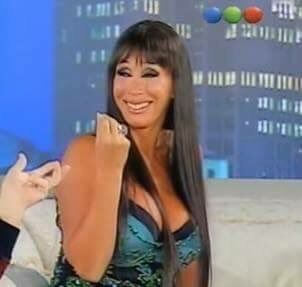
\includegraphics[width=4.19in]{img/moria}

Planteemos otro problema:

Resulta que estas flores son redondas entonces podemos calcular la superficie del pétalo y el sépalo (el ancho es el diámetro no?).

O sea que si hacemos el ancho/2, obtenemos el radio y si lo elevo al cuadrado y lo multiplicamos por pi (3.14) obtenemos la superficie, pero solo de las medidas width!

O sea que ahora no podemos agarrar un rango!, el método phil colins no sirve!!!

Y ahí llega, a salvar las papas \texttt{select()}

\begin{Shaded}
\begin{Highlighting}[]
\NormalTok{superficies}\OtherTok{\textless{}{-}}\NormalTok{flores }\SpecialCharTok{\%\textgreater{}\%} \FunctionTok{select}\NormalTok{(Petal.Width, Sepal.Width)}

\FunctionTok{head}\NormalTok{(superficies)}
\end{Highlighting}
\end{Shaded}

\begin{verbatim}
##   Petal.Width Sepal.Width
## 1         0.2         3.5
## 2         0.2         3.0
## 3         0.2         3.2
## 4         0.2         3.1
## 5         0.2         3.6
## 6         0.4         3.9
\end{verbatim}

Select nos permite tomar un conjunto de columnas que no sean contiguas y ponerlas en otro dataset.
Esquemáticaente algo así:

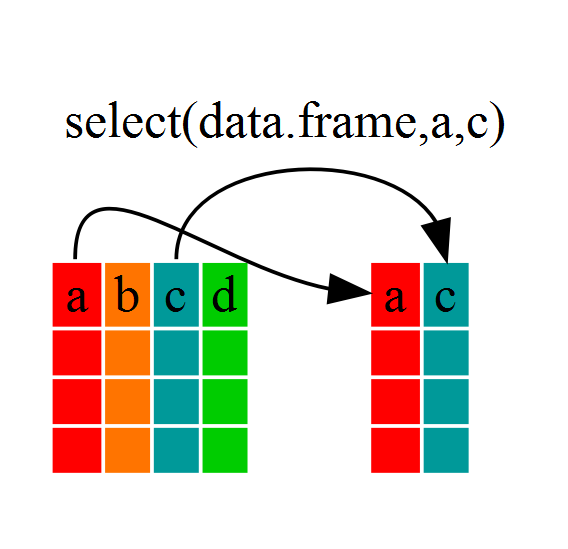
\includegraphics[width=7.89in]{img/select}
Ahora sí podemos proseguir con la transformación:

\begin{Shaded}
\begin{Highlighting}[]
\NormalTok{superficies}\OtherTok{\textless{}{-}}\FloatTok{3.14}\SpecialCharTok{*}\NormalTok{((superficies}\SpecialCharTok{/}\DecValTok{2}\NormalTok{)}\SpecialCharTok{\^{}}\DecValTok{2}\NormalTok{) }\CommentTok{\#transformo en superficies}

\NormalTok{superficies}\SpecialCharTok{$}\NormalTok{especie}\OtherTok{\textless{}{-}}\NormalTok{flores}\SpecialCharTok{$}\NormalTok{Species }\CommentTok{\#le pego la especie}

\FunctionTok{head}\NormalTok{(superficies) }\CommentTok{\#chusmeo}
\end{Highlighting}
\end{Shaded}

\begin{verbatim}
##   Petal.Width Sepal.Width especie
## 1      0.0314     9.61625  setosa
## 2      0.0314     7.06500  setosa
## 3      0.0314     8.03840  setosa
## 4      0.0314     7.54385  setosa
## 5      0.0314    10.17360  setosa
## 6      0.1256    11.93985  setosa
\end{verbatim}

\hypertarget{funciuxf3n-arrange}{%
\subsection{Función arrange()}\label{funciuxf3n-arrange}}

La función arrange es quizàs la más facil de entender, su funcionamiento básico consiste en ordenar las filas de acuerdo a algún criterio (muy similar al ordenar de excel)

Su valor por defecto es el orden ascendente, si quisieramos un orden descendente deberiamos indicarselo, otra ventaja es que podemos ordenar por distintas columnas.

Veamos un ejemplo, queremos ordenar los datos de gapminder para que nos muestre los más viejos y de esos el menor PBI primero:

\begin{Shaded}
\begin{Highlighting}[]
\CommentTok{\# recuerden que anidamos la funcion head }
\CommentTok{\# para no mostrar toooda la base }

\FunctionTok{head}\NormalTok{(data }\SpecialCharTok{\%\textgreater{}\%} \FunctionTok{arrange}\NormalTok{(year, gdpPercap))}
\end{Highlighting}
\end{Shaded}

\begin{verbatim}
## # A tibble: 6 x 6
##   country       continent  year lifeExp      pop gdpPercap
##   <fct>         <fct>     <int>   <dbl>    <int>     <dbl>
## 1 Lesotho       Africa     1952    42.1   748747      299.
## 2 Guinea-Bissau Africa     1952    32.5   580653      300.
## 3 Eritrea       Africa     1952    35.9  1438760      329.
## 4 Myanmar       Asia       1952    36.3 20092996      331 
## 5 Burundi       Africa     1952    39.0  2445618      339.
## 6 Ethiopia      Africa     1952    34.1 20860941      362.
\end{verbatim}

Si quisieramos mostrar al reves, los màs nuevos y de mayor PBI deberíamos apelar al orden descendente

\begin{Shaded}
\begin{Highlighting}[]
\CommentTok{\# recuerden que ustedes pueden usarlo sin la funcion head }

\FunctionTok{head}\NormalTok{(data }\SpecialCharTok{\%\textgreater{}\%} \FunctionTok{arrange}\NormalTok{(}\FunctionTok{desc}\NormalTok{(year), }\FunctionTok{desc}\NormalTok{(gdpPercap)))}
\end{Highlighting}
\end{Shaded}

\begin{verbatim}
## # A tibble: 6 x 6
##   country          continent  year lifeExp       pop gdpPercap
##   <fct>            <fct>     <int>   <dbl>     <int>     <dbl>
## 1 Norway           Europe     2007    80.2   4627926    49357.
## 2 Kuwait           Asia       2007    77.6   2505559    47307.
## 3 Singapore        Asia       2007    80.0   4553009    47143.
## 4 United States    Americas   2007    78.2 301139947    42952.
## 5 Ireland          Europe     2007    78.9   4109086    40676.
## 6 Hong Kong, China Asia       2007    82.2   6980412    39725.
\end{verbatim}

\hypertarget{funciuxf3n-mutate}{%
\section{Función mutate()}\label{funciuxf3n-mutate}}

La función \texttt{mutate()} sirve para crear nuevas variables que son funciones de otras que se encuentran ahí. ¿Se acuerdan del problema de las flores de Fisher?, bueno veamos como esto nos brinda una herramienta mas inteligente para resolverlo.

\begin{Shaded}
\begin{Highlighting}[]
\FunctionTok{rm}\NormalTok{(flores) }\CommentTok{\#borro flores porque le hicimos cambios y queremos empezar de cero}

\NormalTok{flores}\OtherTok{\textless{}{-}}\NormalTok{iris }\CommentTok{\#le asigno el dataset iris y volvimos a foja cero}
\end{Highlighting}
\end{Shaded}

Queremos pasar las medidas a cm, ¿recuerdan? vamos a usar la función \texttt{mutate()} para eso.

\begin{Shaded}
\begin{Highlighting}[]
\NormalTok{flores }\OtherTok{\textless{}{-}}\NormalTok{ flores }\SpecialCharTok{\%\textgreater{}\%} \FunctionTok{mutate}\NormalTok{( }\AttributeTok{Petal.Length.cm =}\NormalTok{ Petal.Length}\SpecialCharTok{*}\FloatTok{2.54}\NormalTok{)}

\FunctionTok{head}\NormalTok{(flores)}
\end{Highlighting}
\end{Shaded}

\begin{verbatim}
##   Sepal.Length Sepal.Width Petal.Length Petal.Width Species Petal.Length.cm
## 1          5.1         3.5          1.4         0.2  setosa           3.556
## 2          4.9         3.0          1.4         0.2  setosa           3.556
## 3          4.7         3.2          1.3         0.2  setosa           3.302
## 4          4.6         3.1          1.5         0.2  setosa           3.810
## 5          5.0         3.6          1.4         0.2  setosa           3.556
## 6          5.4         3.9          1.7         0.4  setosa           4.318
\end{verbatim}

Excelente, pero, ya sabíamos hacer eso, ¿por qué me conviene usar mutate()? Bueno porque nos permite tambien hacer no uno sino muchos cambios en una misma linea de código, así:

\begin{Shaded}
\begin{Highlighting}[]
\NormalTok{flores }\OtherTok{\textless{}{-}}\NormalTok{ flores }\SpecialCharTok{\%\textgreater{}\%} \FunctionTok{mutate}\NormalTok{( }\AttributeTok{Petal.Length.cm =}\NormalTok{ Petal.Length}\SpecialCharTok{*}\FloatTok{2.54}\NormalTok{,}
                             \AttributeTok{Petal.Width.cm =}\NormalTok{ Petal.Width}\SpecialCharTok{*}\FloatTok{2.54}\NormalTok{,}
                             \AttributeTok{Sepal.Length.cm =}\NormalTok{ Sepal.Length}\SpecialCharTok{*}\FloatTok{2.54}\NormalTok{,}
                             \AttributeTok{Sepal.Width.cm =}\NormalTok{ Sepal.Width}\SpecialCharTok{*}\FloatTok{2.54}\NormalTok{,}
\NormalTok{                             )}

\FunctionTok{head}\NormalTok{(flores)}
\end{Highlighting}
\end{Shaded}

\begin{verbatim}
##   Sepal.Length Sepal.Width Petal.Length Petal.Width Species Petal.Length.cm
## 1          5.1         3.5          1.4         0.2  setosa           3.556
## 2          4.9         3.0          1.4         0.2  setosa           3.556
## 3          4.7         3.2          1.3         0.2  setosa           3.302
## 4          4.6         3.1          1.5         0.2  setosa           3.810
## 5          5.0         3.6          1.4         0.2  setosa           3.556
## 6          5.4         3.9          1.7         0.4  setosa           4.318
##   Petal.Width.cm Sepal.Length.cm Sepal.Width.cm
## 1          0.508          12.954          8.890
## 2          0.508          12.446          7.620
## 3          0.508          11.938          8.128
## 4          0.508          11.684          7.874
## 5          0.508          12.700          9.144
## 6          1.016          13.716          9.906
\end{verbatim}

Excelente, pero que ventaja tiene esto por sobre el método de extraerlos en una base, multiplicarlos y después pegarles las que necesitaba, dos muy importantes:

\begin{enumerate}
\def\labelenumi{\arabic{enumi}.}
\item
  el método anterior crea un objeto nuevo (muchos objetos enlentecen el programan y complican al usuario, imaginen que al final del día tienen una base \emph{flores}, una \emph{flores2}, una \emph{floreees}, y una \emph{floresfinal}, y no recuerdan en donde esta cada cosa).
\item
  este método permite aplicar tranformaciones diferentes a un grupo de variables
\end{enumerate}

Veamos esta última opción:

Resulta que queremos calcular el largo en metros del petalo y el sepalo y calcular las superficies como la otra vez, ¿podemos hacerlo todo con una sola función?, claro que sí, gracias a mutate():

\begin{Shaded}
\begin{Highlighting}[]
\NormalTok{flores}\OtherTok{\textless{}{-}}\NormalTok{flores }\SpecialCharTok{\%\textgreater{}\%} \FunctionTok{mutate}\NormalTok{(}\AttributeTok{Petal.Length.m =}\NormalTok{ Petal.Length.cm}\SpecialCharTok{/}\DecValTok{100}\NormalTok{,}
                          \AttributeTok{Sepal.Length.m =}\NormalTok{ Sepal.Length.cm}\SpecialCharTok{/}\DecValTok{100}\NormalTok{,}
                          \AttributeTok{Petal.surface.m =} \FloatTok{3.14}\SpecialCharTok{*}\NormalTok{((Petal.Width.cm}\SpecialCharTok{/}\DecValTok{100}\SpecialCharTok{/}\DecValTok{2}\NormalTok{))}\SpecialCharTok{\^{}}\DecValTok{2}\NormalTok{,}
                          \AttributeTok{Sepal.surface.m =} \FloatTok{3.14}\SpecialCharTok{*}\NormalTok{((Sepal.Width.cm}\SpecialCharTok{/}\DecValTok{100}\SpecialCharTok{/}\DecValTok{2}\NormalTok{))}\SpecialCharTok{\^{}}\DecValTok{2}\NormalTok{)}
\FunctionTok{head}\NormalTok{(flores)                          }
\end{Highlighting}
\end{Shaded}

\begin{verbatim}
##   Sepal.Length Sepal.Width Petal.Length Petal.Width Species Petal.Length.cm
## 1          5.1         3.5          1.4         0.2  setosa           3.556
## 2          4.9         3.0          1.4         0.2  setosa           3.556
## 3          4.7         3.2          1.3         0.2  setosa           3.302
## 4          4.6         3.1          1.5         0.2  setosa           3.810
## 5          5.0         3.6          1.4         0.2  setosa           3.556
## 6          5.4         3.9          1.7         0.4  setosa           4.318
##   Petal.Width.cm Sepal.Length.cm Sepal.Width.cm Petal.Length.m Sepal.Length.m
## 1          0.508          12.954          8.890        0.03556        0.12954
## 2          0.508          12.446          7.620        0.03556        0.12446
## 3          0.508          11.938          8.128        0.03302        0.11938
## 4          0.508          11.684          7.874        0.03810        0.11684
## 5          0.508          12.700          9.144        0.03556        0.12700
## 6          1.016          13.716          9.906        0.04318        0.13716
##   Petal.surface.m Sepal.surface.m
## 1    2.025802e-05     0.006204020
## 2    2.025802e-05     0.004558055
## 3    2.025802e-05     0.005186054
## 4    2.025802e-05     0.004866990
## 5    2.025802e-05     0.006563600
## 6    8.103210e-05     0.007703114
\end{verbatim}

Lo logramos, creamos funciones diferentes, sin crear objetos intermedios y con una sola función!

Creanme a medida que pase el tiempo van a notar lo conveniente de ahorrar lineas de comando y objetos.

\hypertarget{otras-funciones-de-dplyr}{%
\section{Otras funciones de dplyr}\label{otras-funciones-de-dplyr}}

Estas funciones que vimos aquí son quizás las más útiles para empezar pero son sólo la punta del iceberg.
Este paquete tiene muchísimas funciones, seguramente con la práctica vamos a ir conociendo algunas.

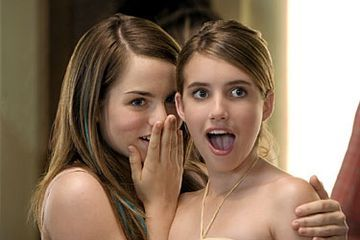
\includegraphics[width=5in]{img/jojo}

Por las dudas aquí tienen un pequeños listado para investigar (spoiler, a esta lista la vamos a usar):

\begin{quote}
\textbf{FUNCIONES DPLYR}

group\_by()\\
if\_else()\\
if\_all()\\
if\_any()\\
mutate\_all()\\
mutate\_if()\\
na\_if()\\
rename()\\
summarise()\\
summarise\_all()
\end{quote}

\hypertarget{ejercicios-2}{%
\section{\texorpdfstring{ Ejercicios:}{ Ejercicios:}}\label{ejercicios-2}}

En esta sección vamos a usar lo que aprendimos (y todo nuestro ingenio y creatividad) para resolver pequeños problemas con la base gapminder.

El desafío: hacerlo con el menor número de lineas y de objetos intermedios.

Empecemos

\hypertarget{problema-1}{%
\subsection{Problema 1:}\label{problema-1}}

En nuestra base hay una variable \texttt{lifeExp} que representa la esperanza de vida en años. Queremos crear una variable nueva que se llame \texttt{lifeExp\_months} y represente la expectativa de vida en meses:

\begin{Shaded}
\begin{Highlighting}[]
\CommentTok{\#}
\CommentTok{\#}
\CommentTok{\#}
\CommentTok{\#}
\CommentTok{\#}
\end{Highlighting}
\end{Shaded}

\hypertarget{problema-2}{%
\subsection{Problema 2:}\label{problema-2}}

Queremos mostrar el país con la mayor población en 1997. Quizas quieran usar varias veces el operador \%\textgreater\%:

\begin{Shaded}
\begin{Highlighting}[]
\CommentTok{\#}
\CommentTok{\#}
\CommentTok{\#}
\CommentTok{\#}
\CommentTok{\#}
\end{Highlighting}
\end{Shaded}

\hypertarget{problema-3}{%
\subsection{Problema 3:}\label{problema-3}}

Vamos afrontar un desafío, quiero crear una base \texttt{mas\_ricos} con los países (en orden ascendente) que en el año 2007 superaron el billón de PBI total (Recuerden \texttt{gdpPercap} es el PBI per cápita y \texttt{pop} es la población total). Traten de hacerlo por uds mismos (pista: recuerden que podemos \emph{pipear} funciones)

\begin{Shaded}
\begin{Highlighting}[]
\CommentTok{\#}
\CommentTok{\#}
\CommentTok{\#}
\CommentTok{\#}
\CommentTok{\#}
\end{Highlighting}
\end{Shaded}

\hypertarget{problema-3-con-mas-pistas}{%
\subsubsection{Problema 3 (con mas pistas):}\label{problema-3-con-mas-pistas}}

Si llegaron hasta acá es porque el ejercicio anterior fue demasiado abrumador (no lo creo). Pero aquí van algunas ayuditas.

Lo primero de lo primero es entender que hay varias condiciones, entonces vamos a tener que \emph{pipear} varias funciones. Ordenemos las condiciones y después las escribimos (recuerden que es muy útil leer el código en voz alta, porque en definitiva es un lenguaje y tiene un sentido).

Primero hay una columna que no existe que debemos crear multiplicando dos existentes (quizas algo relacionado con mutar pueda ser útil ¿no? ), después nos dice que sólo le interesa los datos de 2007 (filtremos por esa condicion) y después sólo los que superan cierto valor (suena como a un segundo filtro) y por último ordenar todo para mostrarlo. Probemos ahora.

\begin{Shaded}
\begin{Highlighting}[]
\CommentTok{\#}
\CommentTok{\#}
\CommentTok{\#}
\CommentTok{\#}
\CommentTok{\#}
\end{Highlighting}
\end{Shaded}

\hypertarget{respuestas}{%
\section{\texorpdfstring{ Respuestas:}{ Respuestas:}}\label{respuestas}}

Esperemos que hayas llegado acá después de haber intentado varias veces encontrar una respuesta por vos mismo. Si no lo hiciste, a subir de nuevo que nada se gana sin luchar (menos aprender).

Si ya te diste por vencido aquí vienen las respuestas:

\textbf{\emph{Importante}}

Recuerden que este es sólo un modo de resolver, hay muchas posibilidades que dependen (entre otras cosas) de su creatividad. No hay un modo correcto pero si hay modos que consumen menos esfuerzo (ahora o en el futuro). La simpleza es siempre el mejor criterio.

\hypertarget{problema-1-1}{%
\subsection{Problema 1:}\label{problema-1-1}}

En nuestra base hay una variable \texttt{lifeExp} que representa la esperanza de vida en años. Queremos crear una variable nueva que se llame \texttt{lifeExp\_months} y represente la expectativa de vida en meses:

\begin{Shaded}
\begin{Highlighting}[]
\NormalTok{data}\OtherTok{\textless{}{-}}\NormalTok{data }\SpecialCharTok{\%\textgreater{}\%} \FunctionTok{mutate}\NormalTok{(}\AttributeTok{lifeExp\_months =}\NormalTok{ lifeExp}\SpecialCharTok{*}\DecValTok{12}\NormalTok{ )}
\end{Highlighting}
\end{Shaded}

\hypertarget{problema-2-1}{%
\subsection{Problema 2:}\label{problema-2-1}}

Queremos mostrar el país con la mayor población en 1997. Quizas quieran usar varias veces el operador \%\textgreater\%:

\begin{Shaded}
\begin{Highlighting}[]
\FunctionTok{head}\NormalTok{(data }\SpecialCharTok{\%\textgreater{}\%} \FunctionTok{filter}\NormalTok{(year}\SpecialCharTok{==}\DecValTok{1997}\NormalTok{) }\SpecialCharTok{\%\textgreater{}\%} \FunctionTok{arrange}\NormalTok{(}\FunctionTok{desc}\NormalTok{(pop)),}\DecValTok{1}\NormalTok{)}
\end{Highlighting}
\end{Shaded}

\begin{verbatim}
## # A tibble: 1 x 7
##   country continent  year lifeExp        pop gdpPercap lifeExp_months
##   <fct>   <fct>     <int>   <dbl>      <int>     <dbl>          <dbl>
## 1 China   Asia       1997    70.4 1230075000     2289.           845.
\end{verbatim}

Vamos a comentar que hicimos acá, leamoslo en vos alta:

A la base data le \textbf{aplique} la opción filtro año=1997, a ese resultado (o sea solo a los registros de 1997) le \textbf{aplique} la función ordernar en orden descendente y todo eso esta \textbf{adentro} de la funcion head() que me muestra los primeros campos de la base, como solo quiero el 1º, le agregué un argumento \texttt{,1} que le dice a la función que sólo presente el primer campo.

\hypertarget{problema-3-1}{%
\subsection{Problema 3:}\label{problema-3-1}}

Vamos afrontar un desafío, quiero crear una base \texttt{mas\_ricos} con los países (en orden ascendente) que en el año 2007 superaron el billón de PBI total (Recuerden \texttt{gdpPercap} es el PBI per cápita y \texttt{pop} es la población total). Traten de hacerlo por uds mismos (pista: recuerden que podemos \emph{pipear} funciones)

\begin{Shaded}
\begin{Highlighting}[]
\NormalTok{mas\_ricos}\OtherTok{\textless{}{-}}\NormalTok{data }\SpecialCharTok{\%\textgreater{}\%} \FunctionTok{mutate}\NormalTok{(}\AttributeTok{PBI =}\NormalTok{ gdpPercap }\SpecialCharTok{*}\NormalTok{ pop ) }\SpecialCharTok{\%\textgreater{}\%} \FunctionTok{filter}\NormalTok{(year }\SpecialCharTok{==} \DecValTok{2007}\NormalTok{) }\SpecialCharTok{\%\textgreater{}\%} \FunctionTok{filter}\NormalTok{(PBI}\SpecialCharTok{\textgreater{}}\DecValTok{1000000000000}\NormalTok{) }\SpecialCharTok{\%\textgreater{}\%} \FunctionTok{arrange}\NormalTok{(PBI)}

\FunctionTok{head}\NormalTok{(mas\_ricos)}
\end{Highlighting}
\end{Shaded}

\begin{verbatim}
## # A tibble: 6 x 8
##   country     continent  year lifeExp       pop gdpPercap lifeExp_months     PBI
##   <fct>       <fct>     <int>   <dbl>     <int>     <dbl>          <dbl>   <dbl>
## 1 Korea, Rep. Asia       2007    78.6  49044790    23348.           943. 1.15e12
## 2 Spain       Europe     2007    80.9  40448191    28821.           971. 1.17e12
## 3 Canada      Americas   2007    80.7  33390141    36319.           968. 1.21e12
## 4 Mexico      Americas   2007    76.2 108700891    11978.           914. 1.30e12
## 5 Italy       Europe     2007    80.5  58147733    28570.           967. 1.66e12
## 6 Brazil      Americas   2007    72.4 190010647     9066.           869. 1.72e12
\end{verbatim}

¿Leemos el código?: a la base data le \textbf{aplique} la tranformacion para calcular el valor del PBI, después a la base resultante le \textbf{aplique} un filtro de año (para quedarme solo con 2007) y después \textbf{aplique} otro filtro para quedarme con los PBIs superiores a un billon, a la resultante le \textbf{aplique} un orden basado en el PBI y a tooodo eso lo \textbf{asigne} a la base \texttt{mas\_ricos}

\begin{quote}
\textbf{Algunos comentarios de estilo }

La forma en que escribimos el código previo es correcta pero un poco desordenada ya que escribimos todo \emph{como un chorizo}

Cuando las lineas son largas conviene partirlas pero al hacer eso debemos dejarle claro a R que despues de esta linea sigue un nuevo argumento, esto solo es posible si dejamos el \%\textgreater\% al final (eso le indica que algo sigue, y lo va a buscar, si no lo encuentra, bueno, termina ahi)

En fin esta es la forma, elegante, de escribirlo:
\end{quote}

\begin{Shaded}
\begin{Highlighting}[]
\NormalTok{mas\_ricos}\OtherTok{\textless{}{-}}\NormalTok{data }\SpecialCharTok{\%\textgreater{}\%} 
  \FunctionTok{mutate}\NormalTok{(}\AttributeTok{PBI =}\NormalTok{ gdpPercap }\SpecialCharTok{*}\NormalTok{ pop ) }\SpecialCharTok{\%\textgreater{}\%} 
  \FunctionTok{filter}\NormalTok{(year }\SpecialCharTok{==} \DecValTok{2007}\NormalTok{) }\SpecialCharTok{\%\textgreater{}\%} 
  \FunctionTok{filter}\NormalTok{(PBI}\SpecialCharTok{\textgreater{}}\DecValTok{1000000000000}\NormalTok{) }\SpecialCharTok{\%\textgreater{}\%} 
  \FunctionTok{arrange}\NormalTok{(PBI)}
\end{Highlighting}
\end{Shaded}

\begin{quote}
Tambien es más cómodo para leer qué funciones se utilizan.

Un objetivo importante es que nuestro código debe ser fácil de leer, esto nos permitirá compartirlo con otros (y que entiendan lo que hicimos).

Recuerden que nuestro código tiene un gran lector esperándolo, nosotros mismos cuando tengamos que contestar al revisor de nuestro artículo. Así que quieránse y dediquense un código agradable a su yo futuro
\end{quote}


\includegraphics[width=9.72in]{img/conspiranoico}

\hypertarget{resumen-de-variables-en-r}{%
\chapter{Resumen de variables en R}\label{resumen-de-variables-en-r}}

La estadística descriptiva (en el sentido amplio del término) es una rama de la estadística cuyo objetivo es resumir, describir y presentar una serie de valores o un conjunto de datos. La estadística descriptiva suele ser el primer paso y una parte importante en cualquier análisis estadístico. Permite comprobar la calidad de los datos y ayuda a ``entender'' los datos al tener una visión clara de los mismos. Si está bien presentada, la estadística descriptiva es clave para permitir a cualquier lector una idea rápida y precisa de nuestro conjunto de datos.

Obviamente la forma en que resumiremos una variable dependerá del tipo de variable que estemos resumiendo.

\hypertarget{resumen-de-variables-categoricas}{%
\section{Resumen de variables categoricas}\label{resumen-de-variables-categoricas}}

Las variables presentadas como categorías se pueden resumir a través de la \textbf{frecuencia} es decir el número de datos que adoptan tal o cual categoría de la variable, la \textbf{frecuencia relativa} es una medida similar pero que tienen en cuenta el número total de observaciones (en pocas palabras es el \emph{porcentaje} de los datos que adoptan tal o cual categoría)

\hypertarget{resumen-de-variables-numuxe9ricas}{%
\section{Resumen de variables numéricas}\label{resumen-de-variables-numuxe9ricas}}

Existen muchas medidas para resumir datos pero en términos generales las vamos a dividir en dos tipos:

\begin{enumerate}
\def\labelenumi{\arabic{enumi}.}
\tightlist
\item
  Medidas de posición y tendencia central
\item
  Medidas de dispersión
\end{enumerate}

Las \emph{medidas de posición} permiten ver ``dónde'' se sitúan los datos, es decir a puntan a valores concretos como ``el medio de los datos'' o ``el mayor de los datos'', por ejemplo.
Las \emph{medidas de tendencia central} son un tipo especial de medidas de posición que nos permiten suponer el valor en donde se encuentra el medio de nuestros datos. Las medidas de posición son:

\begin{itemize}
\tightlist
\item
  Mínimo
\item
  Máximo
\item
  1er, 3er, o 4to cuartil
\item
  \textbf{Media}
\item
  \textbf{Mediana}
\item
  \textbf{Moda}
\end{itemize}

Estas últimas tres son medidas de tendencia central.

Las \emph{medidas de dispersión} permiten a quien las lea generarse una idea de cuan cercanos (o no) estan los valores entre sí y con la medida de tendencia central que lo representa. Las medidas de dispersión más comunes son:

\begin{itemize}
\tightlist
\item
  Desvío estándard
\item
  Varianza
\item
  Intervalo intercuartil
\item
  Coeficiente de variación
\item
  Rango
\end{itemize}

Veamos con un ejemplo sencillo que queremos decir con ello:

Creemos dos sets de números y calculemos sus medias (en este caso una medida de tendencia central.

\begin{Shaded}
\begin{Highlighting}[]
\NormalTok{set1}\OtherTok{\textless{}{-}}\FunctionTok{c}\NormalTok{(}\DecValTok{15}\NormalTok{,}\DecValTok{16}\NormalTok{,}\DecValTok{17}\NormalTok{,}\DecValTok{18}\NormalTok{,}\DecValTok{19}\NormalTok{,}\DecValTok{20}\NormalTok{,}\DecValTok{21}\NormalTok{,}\DecValTok{22}\NormalTok{,}\DecValTok{23}\NormalTok{,}\DecValTok{24}\NormalTok{,}\DecValTok{25}\NormalTok{,}\DecValTok{26}\NormalTok{,}\DecValTok{27}\NormalTok{)}
\NormalTok{set2}\OtherTok{\textless{}{-}}\FunctionTok{c}\NormalTok{(}\DecValTok{7}\NormalTok{,}\DecValTok{9}\NormalTok{,}\DecValTok{11}\NormalTok{,}\DecValTok{13}\NormalTok{,}\DecValTok{15}\NormalTok{,}\DecValTok{17}\NormalTok{,}\DecValTok{19}\NormalTok{,}\DecValTok{21}\NormalTok{,}\DecValTok{23}\NormalTok{,}\DecValTok{25}\NormalTok{,}\DecValTok{27}\NormalTok{,}\DecValTok{29}\NormalTok{,}\DecValTok{31}\NormalTok{,}\DecValTok{33}\NormalTok{,}\DecValTok{35}\NormalTok{)}

\FunctionTok{mean}\NormalTok{(set1)}
\end{Highlighting}
\end{Shaded}

\begin{verbatim}
## [1] 21
\end{verbatim}

\begin{Shaded}
\begin{Highlighting}[]
\FunctionTok{mean}\NormalTok{(set2)}
\end{Highlighting}
\end{Shaded}

\begin{verbatim}
## [1] 21
\end{verbatim}

Son iguales!!!

Ahora veamos como son sus desvíos estándares (medida de dispersión):

\begin{Shaded}
\begin{Highlighting}[]
\FunctionTok{sd}\NormalTok{(set1)}
\end{Highlighting}
\end{Shaded}

\begin{verbatim}
## [1] 3.89444
\end{verbatim}

\begin{Shaded}
\begin{Highlighting}[]
\FunctionTok{sd}\NormalTok{(set2)}
\end{Highlighting}
\end{Shaded}

\begin{verbatim}
## [1] 8.944272
\end{verbatim}

Claramente son distintos, si sólo hubiéramos reportado la medida de tendencia central el lector tendría a pensar que ambas series de casos son iguales sin embargo difieren significativamente en la dispersión de los datos como vimos al crearlas.

La mejor forma de resumir numéricamente una variable es reportando siempre una medida de tendencia central acompañada de una de dispersión.

\hypertarget{antes-de-empezar-1}{%
\section{Antes de empezar}\label{antes-de-empezar-1}}

En este capítulo exploraremos varios paquetes para analizar y resumir nuestros datos en R.

Trabajaremos con los datos del PBI del paquete gapminder y la base iris de Fisher (si llegaron a este capítulo sin leer los anteriores en el capítulo 5 explicamos de donde venían estas bases).

Si ya no tienen estas bases en el ambiente pueden correr las siguientes líneas para tenerlos a mano:

\begin{Shaded}
\begin{Highlighting}[]
\FunctionTok{library}\NormalTok{(}\StringTok{"gapminder"}\NormalTok{)}

\NormalTok{data}\OtherTok{\textless{}{-}}\NormalTok{gapminder}

\NormalTok{flores}\OtherTok{\textless{}{-}}\NormalTok{iris}
\end{Highlighting}
\end{Shaded}

\hypertarget{estaduxedstica-descriptiva-buxe1sica}{%
\section{Estadística descriptiva básica}\label{estaduxedstica-descriptiva-buxe1sica}}

Muchas de las funciones que veremos en este sección las hemos usado intuitivamente en capítulos anteriores así que haremos un repaso a vuelo de pajaro de las mismas.

\hypertarget{medidas-de-posiciuxf3n}{%
\subsection{Medidas de posición}\label{medidas-de-posiciuxf3n}}

\hypertarget{media}{%
\subsubsection{Media}\label{media}}

Desde la secundaria que estamos familiarizados con el concepto de la media o promedio. La media es el resultado de un cálculo aritmético, que nos permite estimar el valor central de los datos o, en otras palabras, el centro de gravedad de los mismos. La media se obtiene sumando todos los valores y dividiendo esta suma por el número de observaciones (denominado \emph{n}).

Vamos a plantear un ejemplo que nos ayude a visualizar mejor porque decimos que es el ``centro de gravedad de los datos''.

Imaginemos que un alumno se saca en estadística un 2, dos 8s y un 10. ¿La media sería de 7, no?. Bueno imaginemos que estamos en una especie de sube y baja con casillas de igual tamaño que representan las notas y cada nota es un pelota. El 7 sería el casillero en donde ambos ``pesos'' quedan equilibrados, o sea donde deberiamos poner el fulcro si queremos que este sube y baja quede balanceado.

Algo así:

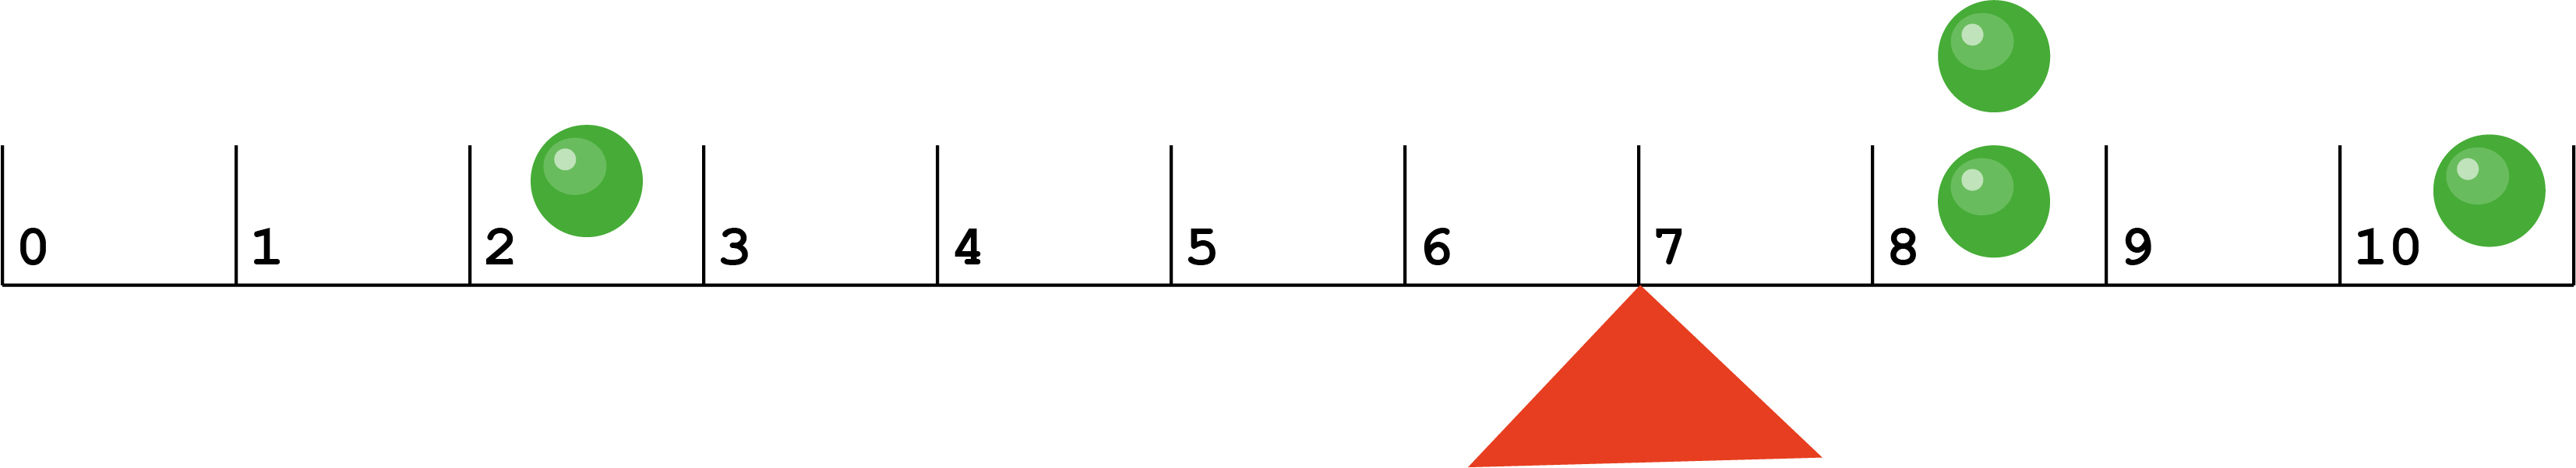
\includegraphics[width=45.92in]{img/mean_ruler}

Como todo estudiante sabe, agregar valores (notas) en los extremos del sube y baja cambia notablemente donde debemos poner el centro de gravedad (porque hacen ``palanca'' en los datos), como si nos sacaramos un 0, en el próximo parcial, la situacion quedaría así:

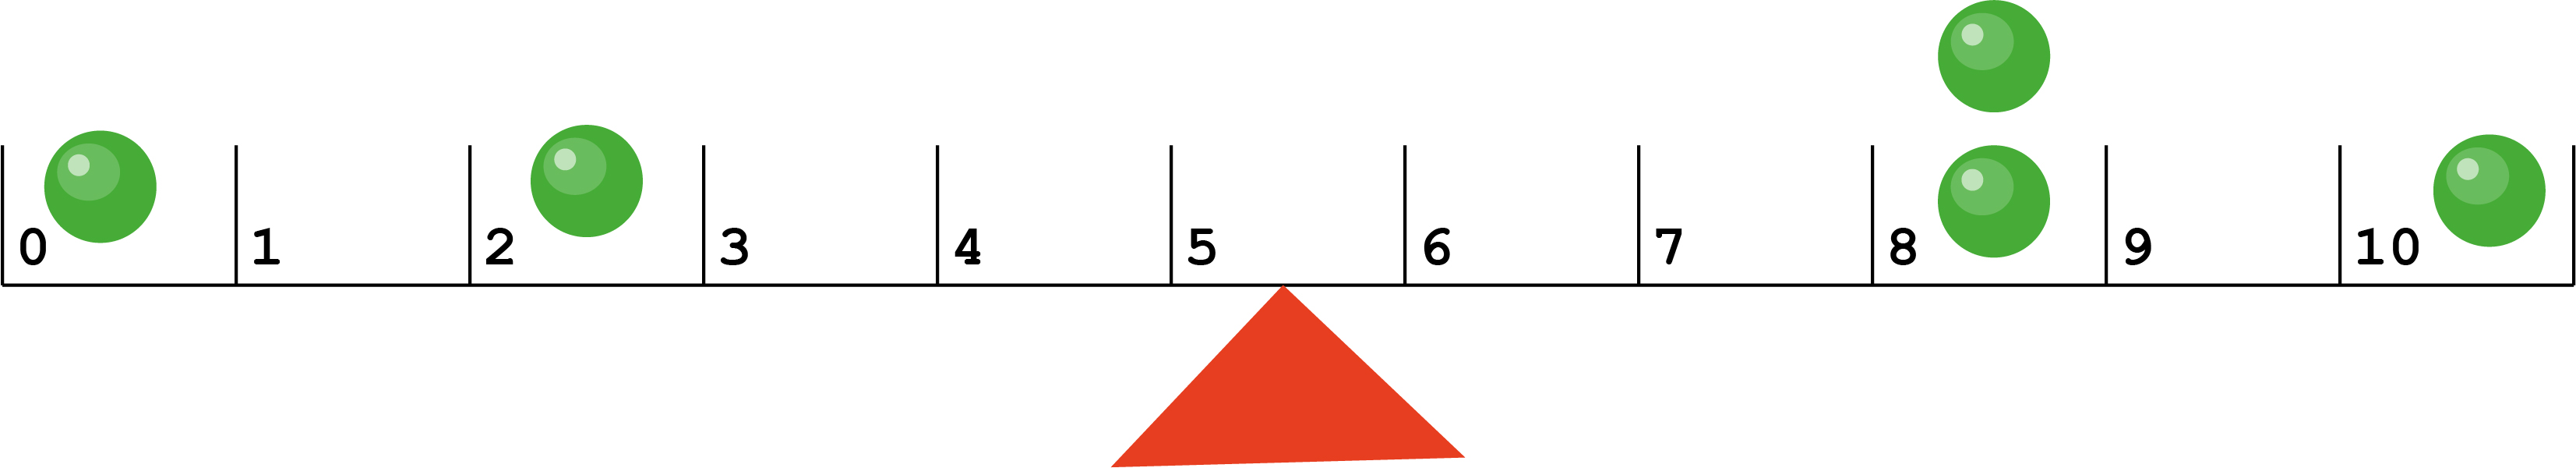
\includegraphics[width=45.92in]{img/mean_ruler_2}

La media sería de 5,6, hubiera variado casi dos puntos en una escala de 10.

Si en cambio la nota siguiente no fuera un 0, sino un valor muy cercano a la media, como un 6 digamos, pasía algo así

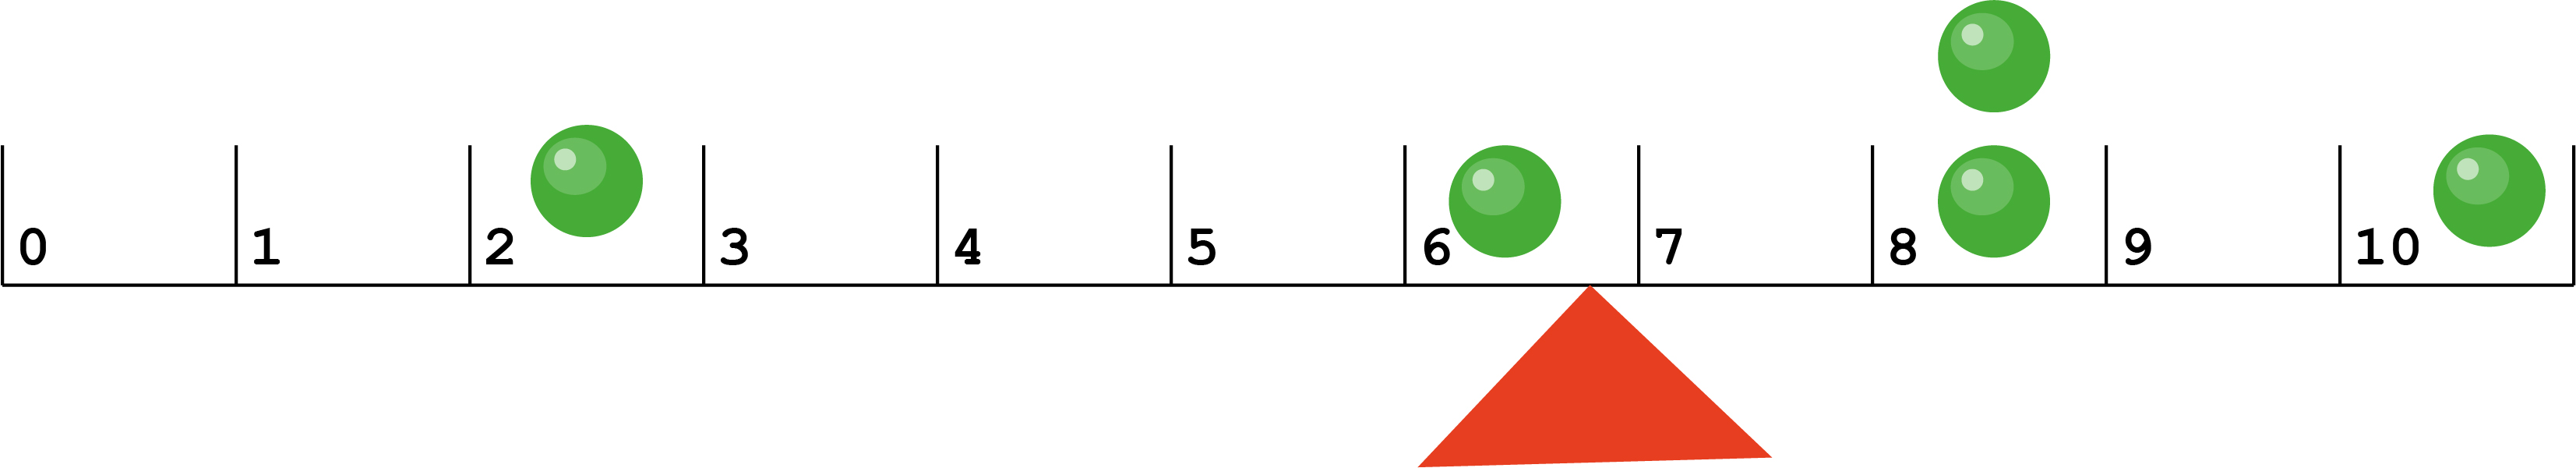
\includegraphics[width=45.92in]{img/mean_ruler_3}

La media hubiera sido de 6,8; es decir prácticamente no se hubiera movido.

Resumiendo, lo que cualquier alumno (o niño que use un sube y baja) sabe, adicionar a la muestra nuevos valores cercanos a la media no la hacen variar prácticamente, mientras que adicionar valores extremos generan una variación enorme (por un efecto de ``apalancamiento'' de los datos). Esta circunstancia hace que la media sea extremadamente susceptible a la aparición de valores atípicos o outliers. Los valores atípicos pueden originarse por una serie de circunstancias (como un error), y son pocos (sino no serían atípicos), si tienen una posición de privilegio en la determinación del centro de los datos puede ser que estemos creando un ``centro atípico'' o falso. Es por esta razón en que la media no siempre es la mejor medida para calcular el centro de una variable.

Bueno una vez que pasamos esta pequeña introducción, veamos como calcularla en R.

Super simple, calculemos la media de el PBI en la base que cargamos:

\begin{Shaded}
\begin{Highlighting}[]
\FunctionTok{mean}\NormalTok{(data}\SpecialCharTok{$}\NormalTok{gdpPercap)}
\end{Highlighting}
\end{Shaded}

\begin{verbatim}
## [1] 7215.327
\end{verbatim}

Un punto \textbf{importante}, si en nuestra base falta aunque sea un sólo valor esta formula da error, a menos que agreguemos un argumento que se lee como ``remover los vacíos''. Y sería algo así.

\begin{Shaded}
\begin{Highlighting}[]
\FunctionTok{mean}\NormalTok{(data}\SpecialCharTok{$}\NormalTok{gdpPercap,}\AttributeTok{na.rm =} \ConstantTok{TRUE}\NormalTok{)}
\end{Highlighting}
\end{Shaded}

\begin{verbatim}
## [1] 7215.327
\end{verbatim}

\hypertarget{mediana}{%
\subsubsection{Mediana}\label{mediana}}

La mediana se interpreta como el valor a partir del cual hay tantas observaciones por debajo como por encima. En otras palabras, el 50\% de las observaciones están por debajo de la mediana y el 50\% de las observaciones están por encima de la mediana.
Se obtiene ordenando los valores de menor a mayor y seleccionando el que ocupa la condición que los divide en dos. A diferencia de la media es muy resistente a los valores atípicos, veamos como funciona en el ejemplo anterior:

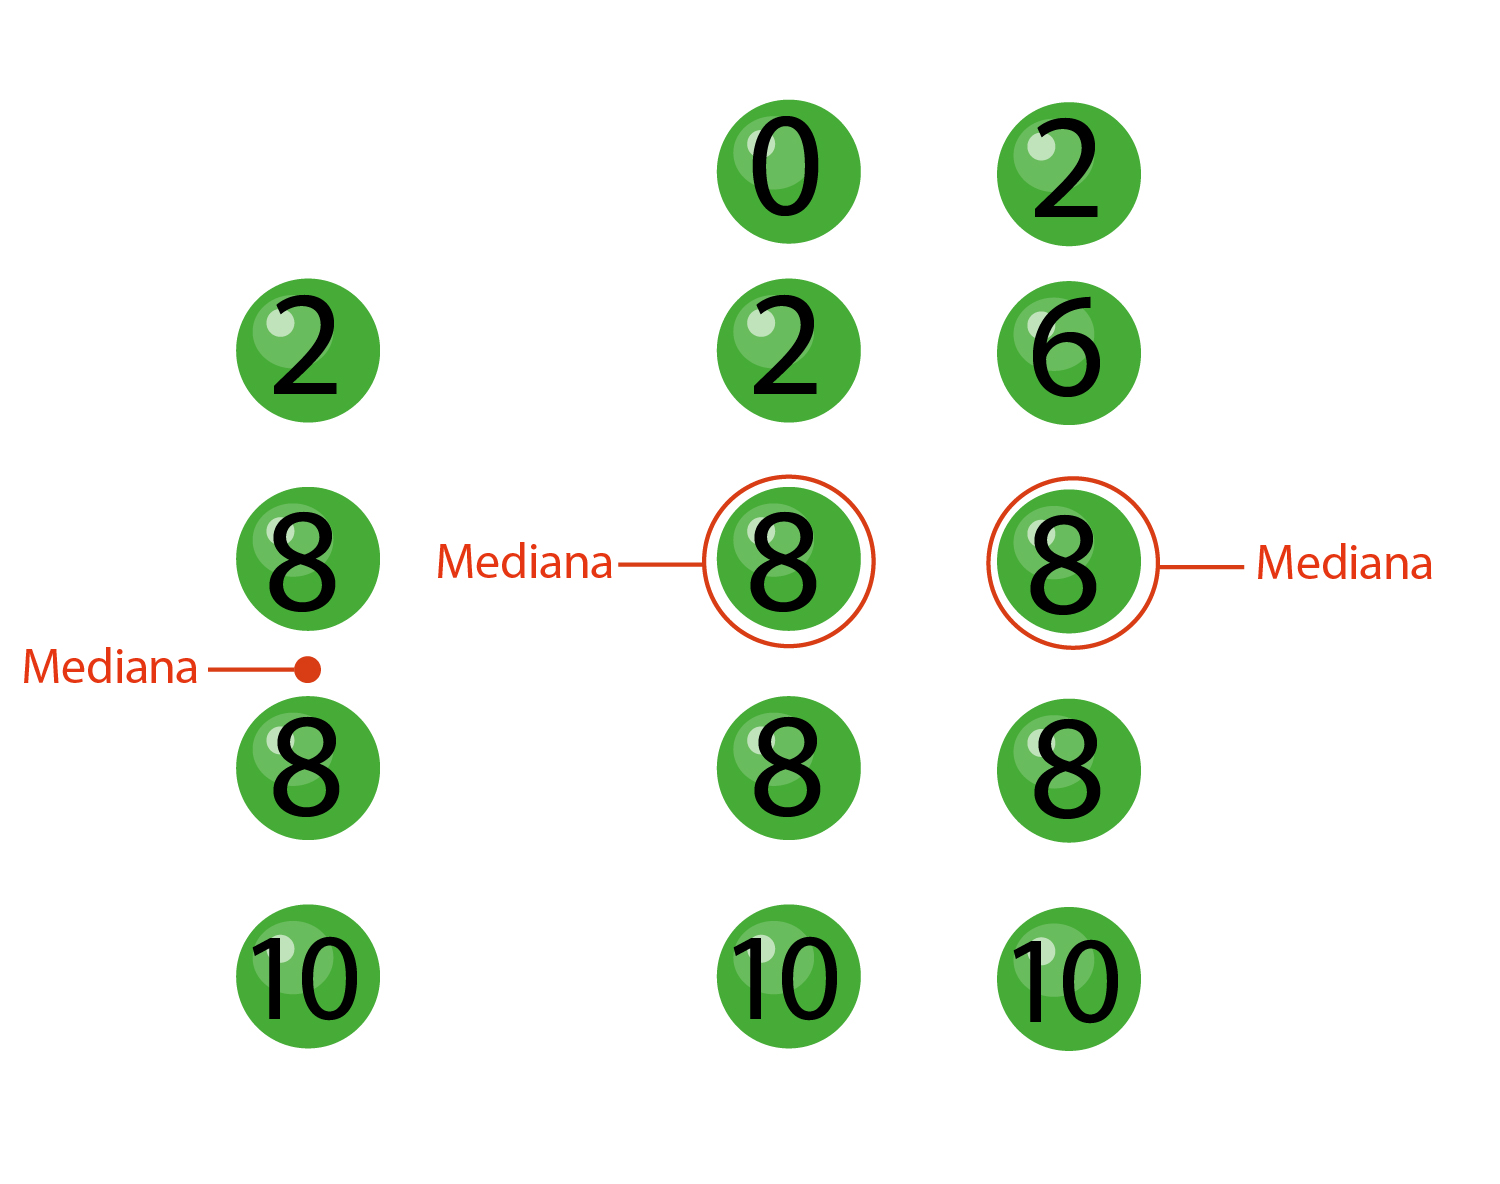
\includegraphics[width=20.83in]{img/median-01}

Como vemos la mediana es una medida mucho mas estable ante los valores extremos.

¿Como la calculamos?

\begin{Shaded}
\begin{Highlighting}[]
\FunctionTok{median}\NormalTok{(data}\SpecialCharTok{$}\NormalTok{gdpPercap,}\AttributeTok{na.rm =} \ConstantTok{TRUE}\NormalTok{)}
\end{Highlighting}
\end{Shaded}

\begin{verbatim}
## [1] 3531.847
\end{verbatim}

\hypertarget{cuartiles}{%
\subsubsection{Cuartiles}\label{cuartiles}}

Si la media es el valor que divide a la muestra (ordenada) en la mitad. Los cuartiles la dividen en cuatro segmentos, el primer cuartil deja un cuarto de la muestra por debajo y 3 por encima, el segundo cuartil dos cuartos por abajo y dos por arriba (si eso les suena igual a dejar media muestra por arriba y media por abajo, es porque sí, el segundo cuartil es la mediana) y el tercer cuartil deja 3 cuartos por debajo y uno por arriba.
Los Percentiles son similares a los cuartiles y dividen la muestra en 100 segmentos (obviamente el percentil 25 es lo mismo que el primer cuartil, el 50 la mediana y el 75 y el tercero)

Los cuartiles se calculan de la siguiente manera

\begin{Shaded}
\begin{Highlighting}[]
\CommentTok{\#si queremos ver todos los cuartiles}
\FunctionTok{quantile}\NormalTok{(data}\SpecialCharTok{$}\NormalTok{gdpPercap) }
\end{Highlighting}
\end{Shaded}

\begin{verbatim}
##          0%         25%         50%         75%        100% 
##    241.1659   1202.0603   3531.8470   9325.4623 113523.1329
\end{verbatim}

\begin{Shaded}
\begin{Highlighting}[]
\CommentTok{\#si sólo queremos el primer cuartil}
\FunctionTok{quantile}\NormalTok{(data}\SpecialCharTok{$}\NormalTok{gdpPercap, }\FloatTok{0.25}\NormalTok{) }
\end{Highlighting}
\end{Shaded}

\begin{verbatim}
##     25% 
## 1202.06
\end{verbatim}

\begin{Shaded}
\begin{Highlighting}[]
\CommentTok{\#o si sólo queremos el tercer cuartil}
\FunctionTok{quantile}\NormalTok{(data}\SpecialCharTok{$}\NormalTok{gdpPercap, }\FloatTok{0.75}\NormalTok{) }
\end{Highlighting}
\end{Shaded}

\begin{verbatim}
##      75% 
## 9325.462
\end{verbatim}

\hypertarget{muxednimo-y-muxe1ximo}{%
\subsubsection{Mínimo y máximo}\label{muxednimo-y-muxe1ximo}}

Definimos como mínimo al valor más pequeño de la muestra y máximo al más grande.
Su calculo es muy sencillo

\begin{Shaded}
\begin{Highlighting}[]
\FunctionTok{min}\NormalTok{(data}\SpecialCharTok{$}\NormalTok{gdpPercap)}
\end{Highlighting}
\end{Shaded}

\begin{verbatim}
## [1] 241.1659
\end{verbatim}

\begin{Shaded}
\begin{Highlighting}[]
\FunctionTok{max}\NormalTok{(data}\SpecialCharTok{$}\NormalTok{gdpPercap)}
\end{Highlighting}
\end{Shaded}

\begin{verbatim}
## [1] 113523.1
\end{verbatim}

\hypertarget{medidas-de-dispersiuxf3n}{%
\subsection{Medidas de dispersión}\label{medidas-de-dispersiuxf3n}}

\hypertarget{rango}{%
\subsubsection{Rango}\label{rango}}

La más simple de las medidas de dispersión, simplemente nos dice cual es la distancia entre el menor y el mayor de los valores.

Existe una función rango, pero nos dice sencillamente el minimo y el maximo (o sea los determinantes del rango)

\begin{Shaded}
\begin{Highlighting}[]
\FunctionTok{range}\NormalTok{(data}\SpecialCharTok{$}\NormalTok{gdpPercap)}
\end{Highlighting}
\end{Shaded}

\begin{verbatim}
## [1]    241.1659 113523.1329
\end{verbatim}

Para calcular el rango propiamente dicho deberiamos restar ambos valores

\begin{Shaded}
\begin{Highlighting}[]
\FunctionTok{max}\NormalTok{(data}\SpecialCharTok{$}\NormalTok{gdpPercap)}\SpecialCharTok{{-}}\FunctionTok{min}\NormalTok{(data}\SpecialCharTok{$}\NormalTok{gdpPercap)}
\end{Highlighting}
\end{Shaded}

\begin{verbatim}
## [1] 113282
\end{verbatim}

\hypertarget{desvuxedo-estuxe1ndard}{%
\subsubsection{Desvío estándard}\label{desvuxedo-estuxe1ndard}}

El desvío estándar es la medida de dispersión más común en estadística. Indica cuál es la desviación ``normal'' de los datos. En realidad, calcula la \emph{desviación promedio} de todos los valores con respecto a la media. Cuanto mayor es la desviación estándar, más dispersos están los datos. Por el contrario, cuanto menor sea la desviación estándar, más centrados estarán los datos en torno a la media.

A continuación una representación visual de la desviación estándar:

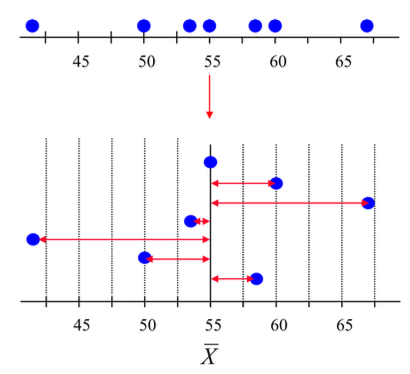
\includegraphics[width=5.69in]{img/SD}

también el cálculo del desvío estándar es muy simple

\begin{Shaded}
\begin{Highlighting}[]
\FunctionTok{sd}\NormalTok{(data}\SpecialCharTok{$}\NormalTok{gdpPercap)}
\end{Highlighting}
\end{Shaded}

\begin{verbatim}
## [1] 9857.455
\end{verbatim}

\hypertarget{intervalo-intercuartil}{%
\subsubsection{Intervalo intercuartil}\label{intervalo-intercuartil}}

El desvío estandard es una medida de dispersión ``basada'' en la media, esto hace que la misma presente los mismos defectos para cierto tipo de muestra. Si necesitáramos usar la mediana para describir mejor a una población, la medida de dispersión que mejor la representa es el \emph{intervalo intercuartil}. Este es la distancia entre el 1er cuartil y el 3ero. De esta forma:

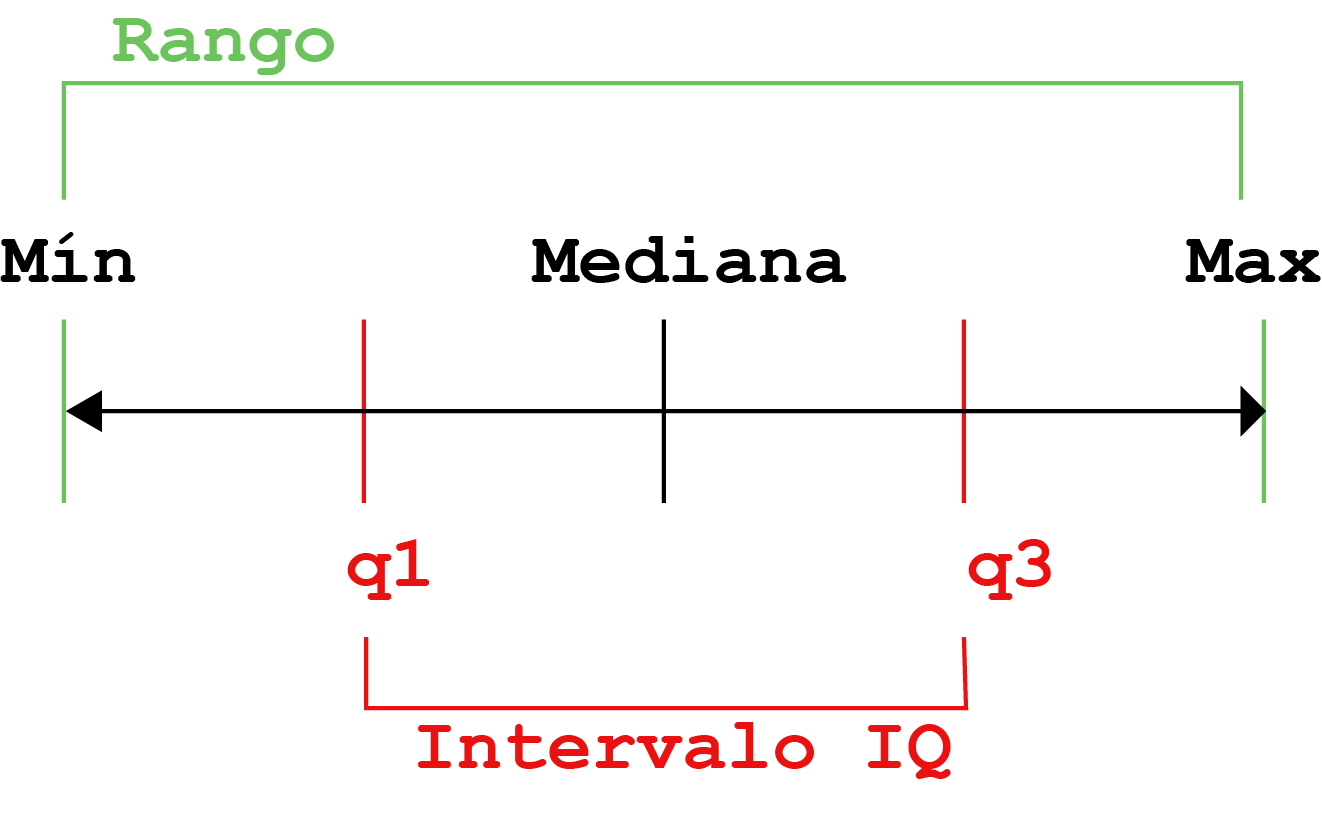
\includegraphics[width=18.36in]{img/IQR}
El cálculo del intervalo intercuartil puede hacerse de la siguiente manera:

\begin{Shaded}
\begin{Highlighting}[]
\FunctionTok{IQR}\NormalTok{(data}\SpecialCharTok{$}\NormalTok{gdpPercap)}
\end{Highlighting}
\end{Shaded}

\begin{verbatim}
## [1] 8123.402
\end{verbatim}

\hypertarget{medidas-de-frecuencia}{%
\subsection{Medidas de frecuencia}\label{medidas-de-frecuencia}}

Como explicáramos antes podemos calcular la frecuencia o la frecuencia relativa de variables categóricas.

La frecuencia absoluta puede obtenerse a traves de la funcion \emph{table()}

\begin{Shaded}
\begin{Highlighting}[]
\FunctionTok{table}\NormalTok{(flores}\SpecialCharTok{$}\NormalTok{Species)}
\end{Highlighting}
\end{Shaded}

\begin{verbatim}
## 
##     setosa versicolor  virginica 
##         50         50         50
\end{verbatim}

Es importante recordar que esta función necesita que nuestra variable categórica este definida como un factor.

Para calcular la frecuencia relativa no existe una función pero podemos recurrir a combinar un par de ellas, sabemos que la función \emph{length()} nos da el numero total de observaciones y sabemos que la frecuencia relativa es el n de esa categoria sobre el n total de observaciones o sea:

\begin{Shaded}
\begin{Highlighting}[]
\FunctionTok{table}\NormalTok{(flores}\SpecialCharTok{$}\NormalTok{Species)}\SpecialCharTok{/}\FunctionTok{length}\NormalTok{(flores}\SpecialCharTok{$}\NormalTok{Species)}
\end{Highlighting}
\end{Shaded}

\begin{verbatim}
## 
##     setosa versicolor  virginica 
##  0.3333333  0.3333333  0.3333333
\end{verbatim}

\hypertarget{tablas-cruzadas}{%
\subsection{Tablas cruzadas}\label{tablas-cruzadas}}

Es frecuente que las variables dicotómicas sean de nuestro interés presentarlas además divididas por grupos, por ejemplo cuantos hombres y mujeres hay entre los casos y entre los controles.

A esto se lo llama \textbf{tablas cruzadas}

Veamos como se puede hacer eso en forma sencilla

Antes que nada para ello necesitamos una base con al menos dos variables categóricas, como nuestras bases de práctica no tienen, vamos a crear una nueva variable y agregarla para poder trabajar, para eso esta línea a continuación:

\begin{Shaded}
\begin{Highlighting}[]
\NormalTok{flores}\SpecialCharTok{$}\NormalTok{origen}\OtherTok{\textless{}{-}}\FunctionTok{sample}\NormalTok{(}\FunctionTok{c}\NormalTok{(}\StringTok{\textquotesingle{}Cortada\textquotesingle{}}\NormalTok{, }\StringTok{\textquotesingle{}Cultivada\textquotesingle{}}\NormalTok{), }\DecValTok{150}\NormalTok{, }\AttributeTok{replace=}\ConstantTok{TRUE}\NormalTok{)}
\end{Highlighting}
\end{Shaded}

(Sólo para satisfacerles la curiosidad, la función \texttt{sample()}crea un vector aleatorio de lo que le pidamos, en este caso cortada o cultivada y el segundo argumento es la cantidad de veces, para meterlo en nuestro dataset lo asigne a una nueva fila con el signo \$)

Bueno ahora que el dataset flores tiene dos variables categóricas podemos hacer una tabla cruzada, para ello la forma más sencilla es usar la función \texttt{table()} pero esta vez con dos argumentos. El orden de los argumentos sigue la eterna lógica de R, primero las filas y después las columnas

\begin{Shaded}
\begin{Highlighting}[]
\FunctionTok{table}\NormalTok{(flores}\SpecialCharTok{$}\NormalTok{Species, flores}\SpecialCharTok{$}\NormalTok{origen)}
\end{Highlighting}
\end{Shaded}

\begin{verbatim}
##             
##              Cortada Cultivada
##   setosa          32        18
##   versicolor      22        28
##   virginica       24        26
\end{verbatim}

\hypertarget{estaduxedstica-descriptiva-en-bloque}{%
\section{Estadística descriptiva en bloque}\label{estaduxedstica-descriptiva-en-bloque}}

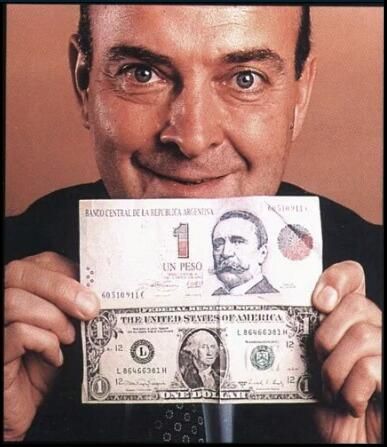
\includegraphics[width=5.38in]{img/mingo}

Como ya habremos aprendido por las malas encarar las cosas 1 a 1, puede traer problemas. En este caso no es para nada cómodo ir evaluando variable por variable cada uno de estos indicadores. Es por eso que en esta sección exploraremos formas simples de analizar un volumen más grande de variables con menos código.

\hypertarget{funciuxf3n-lapply}{%
\subsection{Función lapply()}\label{funciuxf3n-lapply}}

La función \texttt{lapply()} es una función genérica de R que nos permite ``aplicar'' otra función a un conjunto de objeto, esta función tiene una hermana melliza: \texttt{sapply()} que hace fundamentalmente lo mismo pero difieren en la salida (sapply reporta la salida más sencilla y lapply la más informativa), a los efectos que veremos ahora son práctiocamente la misma.

Como dijimos, esta función nos permite aplicar otras funciones a un ``conjunto de objetos'', en este caso vamos a usarla para pedirle que nos de la media de todas las variables numericas de nuestro dataset. Veamos como, la estructura de la función es así \texttt{lapply(list,\ function)}. El primer argumento debe ser una lista de objetos (en este caso las variables) y el segundo la función que queremos que aplique

\begin{Shaded}
\begin{Highlighting}[]
\FunctionTok{lapply}\NormalTok{(data[,}\DecValTok{4}\SpecialCharTok{:}\DecValTok{6}\NormalTok{], mean)}
\end{Highlighting}
\end{Shaded}

\begin{verbatim}
## $lifeExp
## [1] 59.47444
## 
## $pop
## [1] 29601212
## 
## $gdpPercap
## [1] 7215.327
\end{verbatim}

¿Vamos a \emph{leer} que hicimos aquí? Tomamos la función lapply que dice: \emph{a esta lista, hacele esto}; creamos una lista que es las tres columnas de mi data set donde estan expectativa de vida, población y PBI (para eso use el método \emph{phill collins}) y en el segundo argumento le pedi la media

Recuerden que puede que nuestra base tenga valores faltantes, en ese caso la línea de código debería ser así.

\begin{Shaded}
\begin{Highlighting}[]
\FunctionTok{lapply}\NormalTok{(data[,}\DecValTok{4}\SpecialCharTok{:}\DecValTok{6}\NormalTok{], mean, }\AttributeTok{na.rm=}\ConstantTok{TRUE}\NormalTok{)}
\end{Highlighting}
\end{Shaded}

\begin{verbatim}
## $lifeExp
## [1] 59.47444
## 
## $pop
## [1] 29601212
## 
## $gdpPercap
## [1] 7215.327
\end{verbatim}

Este método se puede utilizar para todas las medidas de resumen que vimos en la sección anterior

\begin{Shaded}
\begin{Highlighting}[]
\FunctionTok{lapply}\NormalTok{(data[,}\DecValTok{4}\SpecialCharTok{:}\DecValTok{6}\NormalTok{], mean)}
\end{Highlighting}
\end{Shaded}

\begin{verbatim}
## $lifeExp
## [1] 59.47444
## 
## $pop
## [1] 29601212
## 
## $gdpPercap
## [1] 7215.327
\end{verbatim}

\begin{Shaded}
\begin{Highlighting}[]
\FunctionTok{lapply}\NormalTok{(data[,}\DecValTok{4}\SpecialCharTok{:}\DecValTok{6}\NormalTok{], sd)}
\end{Highlighting}
\end{Shaded}

\begin{verbatim}
## $lifeExp
## [1] 12.91711
## 
## $pop
## [1] 106157897
## 
## $gdpPercap
## [1] 9857.455
\end{verbatim}

\begin{Shaded}
\begin{Highlighting}[]
\FunctionTok{lapply}\NormalTok{(data[,}\DecValTok{4}\SpecialCharTok{:}\DecValTok{6}\NormalTok{], median)}
\end{Highlighting}
\end{Shaded}

\begin{verbatim}
## $lifeExp
## [1] 60.7125
## 
## $pop
## [1] 7023596
## 
## $gdpPercap
## [1] 3531.847
\end{verbatim}

\begin{Shaded}
\begin{Highlighting}[]
\FunctionTok{lapply}\NormalTok{(data[,}\DecValTok{4}\SpecialCharTok{:}\DecValTok{6}\NormalTok{], IQR)}
\end{Highlighting}
\end{Shaded}

\begin{verbatim}
## $lifeExp
## [1] 22.6475
## 
## $pop
## [1] 16791558
## 
## $gdpPercap
## [1] 8123.402
\end{verbatim}

El problema de este método es que si bien nos ahorramos varias líneas de código repetidas (que cuando tenemos una gran base de datos puede ser horas y horas de copy+paste sin sentido) nos permite sólo calcular una medida por vez. Lo mejor de lo mejor sería tener una sóla función para hacer todo, ¿no? Tranquilos que ya va a llegar.

\hypertarget{funciuxf3n-summary}{%
\subsection{Función summary()}\label{funciuxf3n-summary}}

Con esta función estamos familiarizados desde capítulos anteriores así que ya se imaginaran lo sencillo que es (esta vez) poder obtener todas las medidas de cada variable del dataset acorde al tipo de variable que es.

\begin{Shaded}
\begin{Highlighting}[]
\FunctionTok{summary}\NormalTok{(flores)}
\end{Highlighting}
\end{Shaded}

\begin{verbatim}
##   Sepal.Length    Sepal.Width     Petal.Length    Petal.Width   
##  Min.   :4.300   Min.   :2.000   Min.   :1.000   Min.   :0.100  
##  1st Qu.:5.100   1st Qu.:2.800   1st Qu.:1.600   1st Qu.:0.300  
##  Median :5.800   Median :3.000   Median :4.350   Median :1.300  
##  Mean   :5.843   Mean   :3.057   Mean   :3.758   Mean   :1.199  
##  3rd Qu.:6.400   3rd Qu.:3.300   3rd Qu.:5.100   3rd Qu.:1.800  
##  Max.   :7.900   Max.   :4.400   Max.   :6.900   Max.   :2.500  
##        Species      origen         
##  setosa    :50   Length:150        
##  versicolor:50   Class :character  
##  virginica :50   Mode  :character  
##                                    
##                                    
## 
\end{verbatim}

Como verán, esta función es bu-e-ní-si-ma, pero requiere que seamos muy cuidadosos en la definición del tipo de variable previamente. Si miran el resultado de origen pueden ver que no tenemos la frecuencia porque la \emph{clase} de este vector es carácter en lugar de factor. Solucionemoslo:

\begin{Shaded}
\begin{Highlighting}[]
\NormalTok{flores}\SpecialCharTok{$}\NormalTok{origen}\OtherTok{\textless{}{-}}\FunctionTok{as.factor}\NormalTok{(flores}\SpecialCharTok{$}\NormalTok{origen) }\CommentTok{\#cambie la clase del vector}

\FunctionTok{summary}\NormalTok{(flores)}
\end{Highlighting}
\end{Shaded}

\begin{verbatim}
##   Sepal.Length    Sepal.Width     Petal.Length    Petal.Width   
##  Min.   :4.300   Min.   :2.000   Min.   :1.000   Min.   :0.100  
##  1st Qu.:5.100   1st Qu.:2.800   1st Qu.:1.600   1st Qu.:0.300  
##  Median :5.800   Median :3.000   Median :4.350   Median :1.300  
##  Mean   :5.843   Mean   :3.057   Mean   :3.758   Mean   :1.199  
##  3rd Qu.:6.400   3rd Qu.:3.300   3rd Qu.:5.100   3rd Qu.:1.800  
##  Max.   :7.900   Max.   :4.400   Max.   :6.900   Max.   :2.500  
##        Species         origen  
##  setosa    :50   Cortada  :78  
##  versicolor:50   Cultivada:72  
##  virginica :50                 
##                                
##                                
## 
\end{verbatim}

También es cierto que hay algunas medidas (como el IQR) que no están y que deberemos buscar otras estrategias si las necesitamos, como \texttt{lapply()} o ir una por una.

Hemos avanzado muchísimo pero se nos abre ante nosotros un largo viaje, estas medidas de resumen son usualmente utilizadas por los investigadores para mostrarle a sus lectores como es su muestra, esto generalmente se hace en la famosa \textbf{tabla 1} de un paper, cerraremos este capítulo con instrucciones para hacerlo pero antes nos esperan \textbf{ejercicios integradores} y aprender una herramienta más,el diagnóstico de \textbf{parametricidad}

\hypertarget{ejercicios-3}{%
\section{\texorpdfstring{ Ejercicios:}{ Ejercicios:}}\label{ejercicios-3}}

Para estos ejercicios vamos a trabajar con un nuevo dataset ``cars'', incluido en un paquete a instalar lleno de datasets de práctica el paquete se llama ``datasets''.

Dicho dataset contiene datos indican de velocidad de coches y las distancias que tardan en detenerse. Tengan en cuenta que los datos se registraron en la década de 1920 (no se escandalicen).

Nuestro ejercicio consiste en

\begin{enumerate}
\def\labelenumi{\arabic{enumi}.}
\item
  Instalar el paquete ``datasets''
\item
  Activar el paquete
\item
  Asignar la base de datos ``cars'' al objeto data
\end{enumerate}

Y responder las siguientes preguntas:

\begin{enumerate}
\def\labelenumi{\arabic{enumi}.}
\setcounter{enumi}{3}
\item
  ¿Cuántos registros tiene?
\item
  ¿Cual es la velocidad media dentro del dataset?
\item
  ¿y la maxima?
\item
  ¿Cuál es la velocidad media de los primeros 25 registros del dataset?
\end{enumerate}

\hypertarget{respuestas-1}{%
\section{\texorpdfstring{ Respuestas:}{ Respuestas:}}\label{respuestas-1}}

Bueno aquí van nuestars respuestas (recuerden que no hay un sólo modo de hacer las cosas, este es el nuestro)

\begin{Shaded}
\begin{Highlighting}[]
\FunctionTok{library}\NormalTok{(datasets)}

\NormalTok{data}\OtherTok{\textless{}{-}}\NormalTok{cars}

\FunctionTok{str}\NormalTok{(data) }\CommentTok{\# me permite concoer la base y saber cuantos registros hay}
\end{Highlighting}
\end{Shaded}

\begin{verbatim}
## 'data.frame':    50 obs. of  2 variables:
##  $ speed: num  4 4 7 7 8 9 10 10 10 11 ...
##  $ dist : num  2 10 4 22 16 10 18 26 34 17 ...
\end{verbatim}

\begin{Shaded}
\begin{Highlighting}[]
\FunctionTok{mean}\NormalTok{(data}\SpecialCharTok{$}\NormalTok{speed)}
\end{Highlighting}
\end{Shaded}

\begin{verbatim}
## [1] 15.4
\end{verbatim}

\begin{Shaded}
\begin{Highlighting}[]
\FunctionTok{max}\NormalTok{(data}\SpecialCharTok{$}\NormalTok{speed)}
\end{Highlighting}
\end{Shaded}

\begin{verbatim}
## [1] 25
\end{verbatim}

\begin{Shaded}
\begin{Highlighting}[]
\FunctionTok{summary}\NormalTok{(cars) }\CommentTok{\#una forma de contestar dos preguntas más rápido}
\end{Highlighting}
\end{Shaded}

\begin{verbatim}
##      speed           dist       
##  Min.   : 4.0   Min.   :  2.00  
##  1st Qu.:12.0   1st Qu.: 26.00  
##  Median :15.0   Median : 36.00  
##  Mean   :15.4   Mean   : 42.98  
##  3rd Qu.:19.0   3rd Qu.: 56.00  
##  Max.   :25.0   Max.   :120.00
\end{verbatim}

\begin{Shaded}
\begin{Highlighting}[]
\FunctionTok{mean}\NormalTok{(data[}\DecValTok{1}\SpecialCharTok{:}\DecValTok{25}\NormalTok{,}\DecValTok{1}\NormalTok{]) }\CommentTok{\#nos aprovechamos del método "Phil Collins"}
\end{Highlighting}
\end{Shaded}

\begin{verbatim}
## [1] 11.08
\end{verbatim}

\hypertarget{parametricidad}{%
\section{Parametricidad}\label{parametricidad}}

Como seguramente habran visto en la clase del curso que complementa este libro, que una muestra o población siga una distribución normal o Gaussiana es un prerrequisito importante para el uso de ciertas medidas de resumen (como la media) y de varios test de comparación (como el test t)

Por ello es importante que antes de empezar a trabajar podamos estar seguros del cumplimiento de este requisito (veremos mas adelante que el nombre adecuado es \emph{supuesto})

Para diagnosticar la normalidad de una variable se pueden recurrir a:

\begin{enumerate}
\def\labelenumi{\arabic{enumi}.}
\tightlist
\item
  Métodos gráficos
\end{enumerate}

\begin{itemize}
\tightlist
\item
  Histograma
\item
  Boxplot
\item
  Gráficos de densidad
\item
  QQ plot
\end{itemize}

\begin{enumerate}
\def\labelenumi{\arabic{enumi}.}
\setcounter{enumi}{1}
\tightlist
\item
  Métodos analíticos
\end{enumerate}

\begin{itemize}
\tightlist
\item
  Test de komogoroiv smirnof
\item
  Tets de Shapiro Wilk
\end{itemize}

\hypertarget{muxe9todos-gruxe1ficos}{%
\subsection{Métodos gráficos:}\label{muxe9todos-gruxe1ficos}}

\textbf{Histograma}

Los historgramas pueden ser una de las estrategias más sencillas para evaluar si una variable sigue una distribución normal, como vemos en estos ejemplos es facil darse cuenta cuando no, fundamentalmente porque son una medida indirecta de la densidad (la linea que a veces se suma a los histogramas)

Los histogramas pueden hacerse en forma sencilla con la función \texttt{hist()}

\begin{Shaded}
\begin{Highlighting}[]
\FunctionTok{hist}\NormalTok{(flores}\SpecialCharTok{$}\NormalTok{Sepal.Width)}
\end{Highlighting}
\end{Shaded}

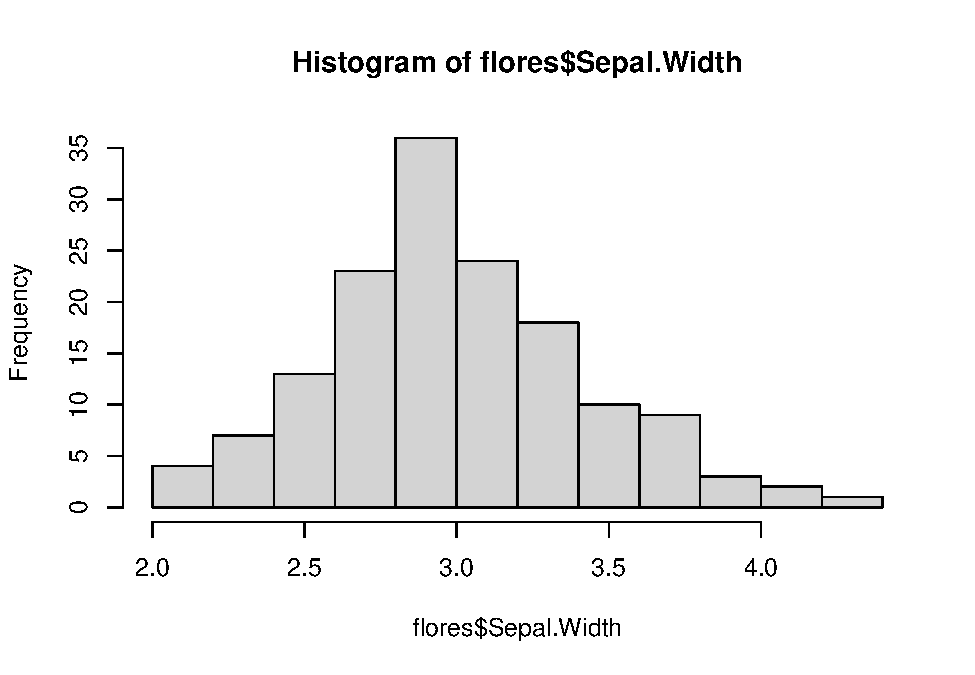
\includegraphics{Esatadistica_en_R_files/figure-latex/unnamed-chunk-122-1.pdf}

Si quisieramos agregar una líneas de densidad podríamos verlo así:

\begin{Shaded}
\begin{Highlighting}[]
\FunctionTok{hist}\NormalTok{(flores}\SpecialCharTok{$}\NormalTok{Sepal.Width, }
 \AttributeTok{prob =} \ConstantTok{TRUE}\NormalTok{)}
\FunctionTok{lines}\NormalTok{(}\FunctionTok{density}\NormalTok{(flores}\SpecialCharTok{$}\NormalTok{Sepal.Width))}
\end{Highlighting}
\end{Shaded}

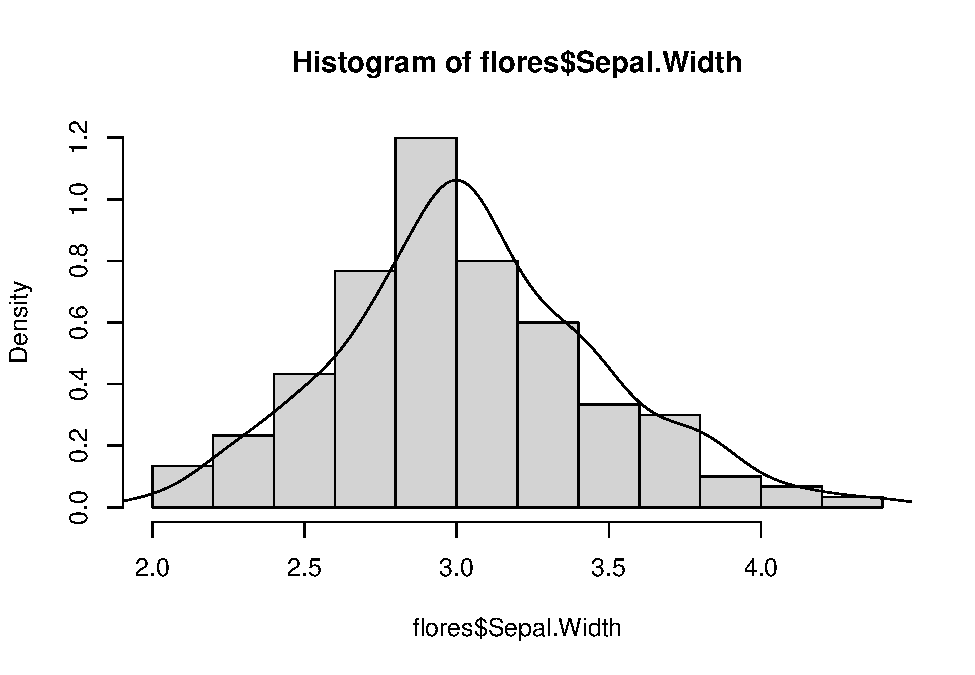
\includegraphics{Esatadistica_en_R_files/figure-latex/unnamed-chunk-123-1.pdf}
Los histogramas permiten decidir si una distribución se acerca a la forma de la normal o no.

Veamos este caso, aquí vemos una distribución (un caso extremo) que no cumple criterios para ser considerada normal, cuando la mayoría de los datos se distribuyen a la izquierda (en valores bajos del eje x) hablamos de distribución desviada a la izquierda (o de colas pesadas por su forma en los box plots) como es el ejemplo de la siguiente. Estas distribuciones son frecuentemente resultado de distribuciones teóricas logarítimicas. Otras variables con comportamiento exponencial, como los casos acumulados de covid, producen distribuciones desviadas a la derecha. Como muchos de ustedes intuirán, describir el numero de casos acumulados de covid con la media desde el inicio de la pandemia no es un enfoque ``representativo''

\begin{Shaded}
\begin{Highlighting}[]
\FunctionTok{library}\NormalTok{(stats)}
\NormalTok{desv\_izq}\OtherTok{\textless{}{-}}\FunctionTok{rlnorm}\NormalTok{(}\DecValTok{600}\NormalTok{, }\AttributeTok{meanlog =}\DecValTok{20}\NormalTok{ , }\AttributeTok{sdlog =} \DecValTok{1}\NormalTok{)}
\FunctionTok{hist}\NormalTok{(desv\_izq)}
\end{Highlighting}
\end{Shaded}

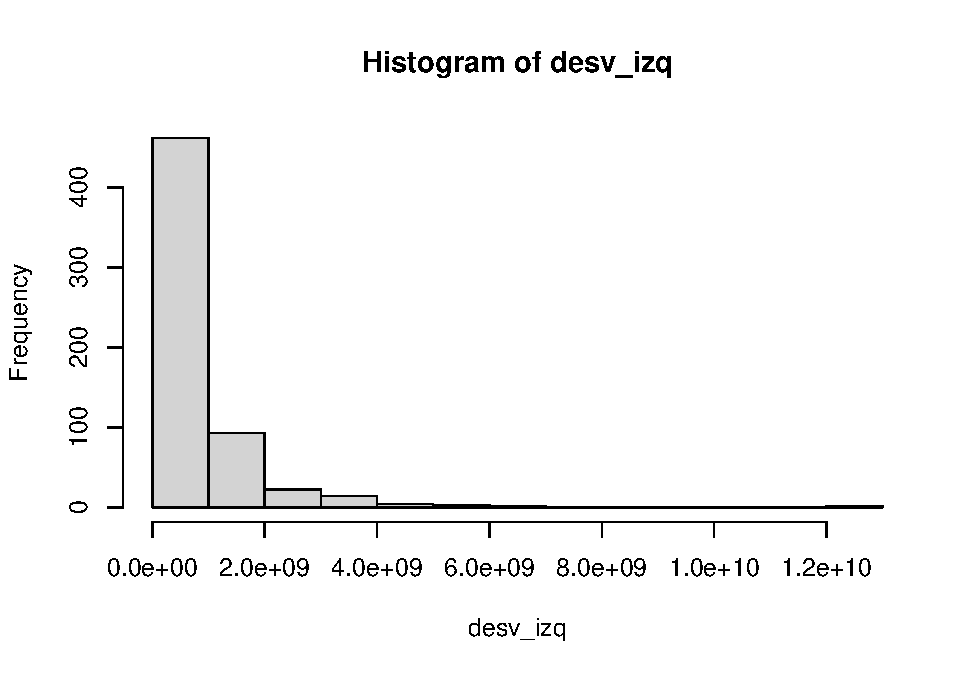
\includegraphics{Esatadistica_en_R_files/figure-latex/unnamed-chunk-124-1.pdf}

\textbf{Box plot}

Los gráficos de box plot o como se llaman en español ``gráficos de caja'' o ``diagramas de cajas y bigotes'', son una forma muy útil de graficar varios parámetros de la distribución que permiten diagnosticar su ``grado de normalidad''. El gráfico consiste en una caja cuyos límites superior son el 1er. cuartil (Q1) y el 3 cuartil (Q3) -por lo tanto la caja es tan alta como el rango intercuartil (RIC), la mediana se grafica comoo una linea dentro de la caja. El gráfico incluye los ``bigotes'' cuyo largo representa el rango total de la variable o 1.5 el RIC sobre o por debajo de Q1 y Q3 (lo que ocurra antes). Eventualmente se puede graficar la media con un asterisco para ver su coincidencia con la mediana.\\
Los valores que pueden quedar por debajo o por encima de los bigotes se les clasifica como ``atípicos'' y se grafican por separado. Los atípicos pueden o no ser outliers (un concepto más complejo).

Estos valores son homologables al histograma aunque es más preciso para

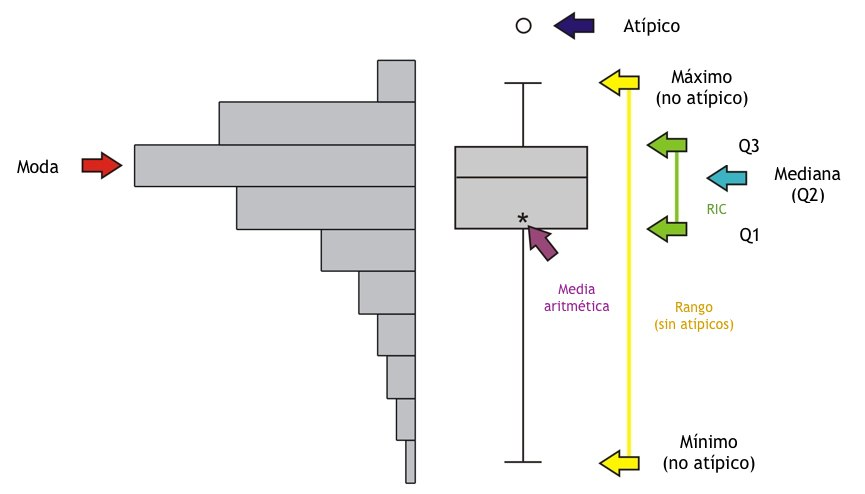
\includegraphics[width=12.01in]{img/box}

Cuando una distribución presenta demasiados valores a la izquierda el bigote se hace muy largo hacia abajo, como si pesara, a estas distribuciones las llamamos de ``colas pesadas'', y en el caso de las desviadas a la izquierda son de ``colas livianas''

Veamos como se construye con nuestros datos

\begin{Shaded}
\begin{Highlighting}[]
\FunctionTok{boxplot}\NormalTok{(flores}\SpecialCharTok{$}\NormalTok{Sepal.Width)}
\end{Highlighting}
\end{Shaded}

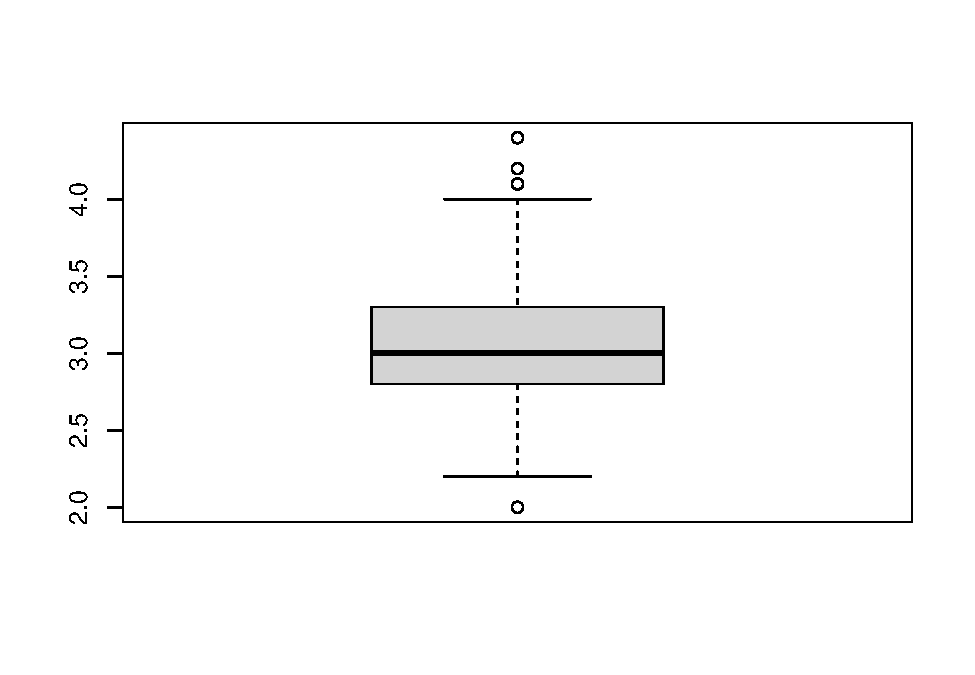
\includegraphics{Esatadistica_en_R_files/figure-latex/unnamed-chunk-126-1.pdf}

\textbf{QQ plot}

El gráfico Q-Q normal o QQ plot es un método gráfico de evaluación de la normalidad alternativo al histograma y es muy útil en tamaños de muestra pequeños (en donde los histogramas suelen verse ``feos'', al graficar). Se llama así para abrevir su nombre correcto que sería ``gráfico (plot) cuantil (Q) a cuantil (Q)''.
En este tipo de gràficos se grafica la dispersión de cada dato sobre el supuesto de una distribución normal perfecta.\\
Esto se logra dividiendo la muestra en múltiples cuantiles y la distribución normal teórica de esa muestra de la misma forma. Si la muestra es ``perfectamente'' normal, cada cuantil muestral es igual a un cuantil teórico y se vería como una linea recta con pendiente 1 (y=x). En los qqplots se grafica esta situación ``ideal'' (en una recta) junto con la situación ``real'' (como puntos)

Para que los datos se consideren normalmente distribuidos, la dispersión debe estar lo más cerca posible de la línea ``ideal'', sin que haya un patrón evidente que se aleje de ella. Veamos como se construye uno con nuestros datos

\begin{Shaded}
\begin{Highlighting}[]
\FunctionTok{library}\NormalTok{(stats)}
\FunctionTok{qqnorm}\NormalTok{(flores}\SpecialCharTok{$}\NormalTok{Sepal.Width, }\AttributeTok{pch =} \DecValTok{1}\NormalTok{, }\AttributeTok{frame =} \ConstantTok{FALSE}\NormalTok{) }\CommentTok{\#esta línea grafica los puuntos}
\FunctionTok{qqline}\NormalTok{(flores}\SpecialCharTok{$}\NormalTok{Sepal.Width, }\AttributeTok{col =} \StringTok{"steelblue"}\NormalTok{, }\AttributeTok{lwd =} \DecValTok{2}\NormalTok{) }\CommentTok{\# esta línea grafica la línea teórica}
\end{Highlighting}
\end{Shaded}

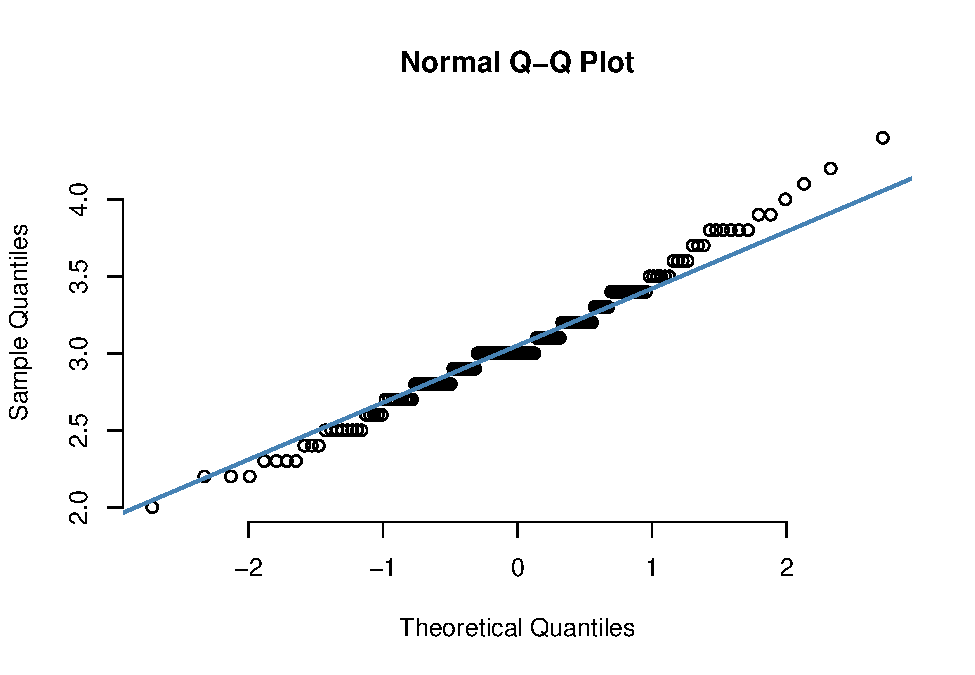
\includegraphics{Esatadistica_en_R_files/figure-latex/unnamed-chunk-127-1.pdf}

\hypertarget{muxe9todos-analuxedticos}{%
\subsection{Métodos analíticos:}\label{muxe9todos-analuxedticos}}

También existen test analíticos específicos para comprobar la normalidad. Es importante tener en cuenta que el mejor enfoque es utilizar màs de un mètodo y convinar mètodos analíticos y gràficos. Esto último se debe a que la mayoría de las pruebas son sensibles a los valores atípicos y están influenciadas por el tamaño de la muestra.

Los test más importantes para la demostración de normalidad son \textbf{el test de Kolmogorov-Smirnov} y \textbf{la prueba W de Shapiro-Wilk}.

\textbf{\emph{Importante}}

Ambas pruebas tienen como hipótesis nula: \emph{los datos se distribuyen normalmente}. Esto quiere decir que \textbf{si p\textgreater{} 0,05, se puede suponer la normalidad.}
Esto puede sonar a veces contraintuitivo y por lo tanto es importante recordarlo siempre

Ambos test son útiles pero existen algunos criterios para preferir uno o el otro:

\begin{itemize}
\item
  Para muestras más pequeñas, es \emph{menos probable} que se detecte la no normalidad. Por esto, es preferible usar la prueba de Shapiro-Wilk, ya que suele ser más sensible.
\item
  Para muestras más grandes (\textgreater{} 100), las pruebas de normalidad son demasiado conservadoras y la hipótesis de normalidad suele rechazarse con demasiada facilidad (razón por la cual hay que acompañarla de mètodos gráficos). En estos casos Kolmogorov-Smirnov es preferioble por su especificidad
\item
  La prueba de Kolmogorov-Smirnov sirve para comparar distribuciones (una real con una teórica, o dos reales entre sí). Para calcular la parametricidad debemos aclarar que la prueba compara la distribución de mis datos con la teórica normal
\end{itemize}

\begin{Shaded}
\begin{Highlighting}[]
\FunctionTok{library}\NormalTok{(stats) }\CommentTok{\#estos test se encuentran dentro del paquete stats}
\FunctionTok{shapiro.test}\NormalTok{(flores}\SpecialCharTok{$}\NormalTok{Sepal.Width)}
\end{Highlighting}
\end{Shaded}

\begin{verbatim}
## 
##  Shapiro-Wilk normality test
## 
## data:  flores$Sepal.Width
## W = 0.98492, p-value = 0.1012
\end{verbatim}

\begin{Shaded}
\begin{Highlighting}[]
\FunctionTok{ks.test}\NormalTok{(flores}\SpecialCharTok{$}\NormalTok{Sepal.Width, }\StringTok{"rnorm"}\NormalTok{) }\CommentTok{\# el argumento "rnorm" indica que el K{-}S compara con la teórica normal}
\end{Highlighting}
\end{Shaded}

\begin{verbatim}
## 
##  One-sample Kolmogorov-Smirnov test
## 
## data:  flores$Sepal.Width
## D = 3.3479, p-value < 2.2e-16
## alternative hypothesis: two-sided
\end{verbatim}

\hypertarget{resumen-de-parametricidad}{%
\subsection{Resumen de parametricidad}\label{resumen-de-parametricidad}}

Como vimos hay varias formas de testearlo (ninguna definitiva), a lo largo de esta sección vimos el analisis de una sola variable en todos los métodos. Al llegar aquí han notado seguramente que tenemos resultados \emph{``contradictorios''}. ¿Qué hacer en estos casos? Bueno, utilizar los conocimientos adquiridos y tomar una \emph{decisión}. Recordemos: a) combinar graficos con analíticos, b) decidir el analítico que mejor se ajusta al problema c) saber que toda decisión implica un margen de error que hay que tolerar.

En este caso nos la jugaremos por decir que la variable Sepal.width tiene un grado de parametricidad ``tolerable''

\hypertarget{la-tabla-1}{%
\section{La tabla 1}\label{la-tabla-1}}

Bueno ha llegado el momento, vamos a estructurar los datos en estadísticas de resumen en un formato agradable para pegar en nuestro paper. Vamos a ver dos paquetes muy útiles para ello.

\textbf{\emph{Importante}}
Al llegar a este punto es importante que todas nuestras variables tengan su correcta \textbf{definición de clase} (Si no recurdan/saben que es esto visiten el capítulo 3.3.2). Los paquetes automatizados para la creación de tablas van a \emph{decidir} como resumir las variables en función del tipo que son (como vimos al inicio de este capítulo de resumen de los datos)

\hypertarget{paquete-table1}{%
\subsection{Paquete table1}\label{paquete-table1}}

El paquete table1 crea tablas html de aspecto profesional, les permite resumir variables en uno o varios grupos y tiene una sintaxis muy sencilla

Como deciamos la sintaxis de table1 es muy sencilla, necesita (en este orden):

\begin{itemize}
\item
  Las lista de las variables, inicia con una virgulilla (es este símbolo, \textasciitilde) y separadas por un +
\item
  La variable que los divide en grupos (si no los hay dejarla vacia) detrás de una barra recta \textbar{}
\item
  El nombre de la base de datos detrás de una ,
\end{itemize}


\includegraphics[width=6.94in]{img/virgu}

veamos que significa esto, vamos a construir una tabla que tenga el ancho y el alto del petalo y el sepalo por especie de nuestra base de flores la sintaxis sería mas o menos asi

\begin{quote}
table1(\textasciitilde Sepal.Length+Sepal.Width+Petal.Length+Petal.Width+origen\textbar Species, flores )
\end{quote}

¿Leemos el código? A las variables \emph{Sepal.Length}, \emph{Sepal.Width}, \emph{Petal.Length}, \emph{Petal.Width} y \emph{origen} agrupémoslas en sus \emph{species} y todos los datos saquemoslos de la base \emph{flores}

Veamos que obtenemos

\begin{Shaded}
\begin{Highlighting}[]
\FunctionTok{library}\NormalTok{(table1)}
\end{Highlighting}
\end{Shaded}

\begin{verbatim}
## 
## Attaching package: 'table1'
\end{verbatim}

\begin{verbatim}
## The following objects are masked from 'package:base':
## 
##     units, units<-
\end{verbatim}

\begin{Shaded}
\begin{Highlighting}[]
\FunctionTok{table1}\NormalTok{(}\SpecialCharTok{\textasciitilde{}}\NormalTok{Sepal.Length}\SpecialCharTok{+}\NormalTok{Sepal.Width}\SpecialCharTok{+}\NormalTok{Petal.Length}\SpecialCharTok{+}\NormalTok{Petal.Width}\SpecialCharTok{+}\NormalTok{origen}\SpecialCharTok{|}\NormalTok{Species, flores )}
\end{Highlighting}
\end{Shaded}

\begin{verbatim}
## [1] "<table class=\"Rtable1\">\n<thead>\n<tr>\n<th class='rowlabel firstrow lastrow'></th>\n<th class='firstrow lastrow'><span class='stratlabel'>setosa<br><span class='stratn'>(N=50)</span></span></th>\n<th class='firstrow lastrow'><span class='stratlabel'>versicolor<br><span class='stratn'>(N=50)</span></span></th>\n<th class='firstrow lastrow'><span class='stratlabel'>virginica<br><span class='stratn'>(N=50)</span></span></th>\n<th class='firstrow lastrow'><span class='stratlabel'>Overall<br><span class='stratn'>(N=150)</span></span></th>\n</tr>\n</thead>\n<tbody>\n<tr>\n<td class='rowlabel firstrow'><span class='varlabel'>Sepal.Length</span></td>\n<td class='firstrow'></td>\n<td class='firstrow'></td>\n<td class='firstrow'></td>\n<td class='firstrow'></td>\n</tr>\n<tr>\n<td class='rowlabel'>Mean (SD)</td>\n<td>5.01 (0.352)</td>\n<td>5.94 (0.516)</td>\n<td>6.59 (0.636)</td>\n<td>5.84 (0.828)</td>\n</tr>\n<tr>\n<td class='rowlabel lastrow'>Median [Min, Max]</td>\n<td class='lastrow'>5.00 [4.30, 5.80]</td>\n<td class='lastrow'>5.90 [4.90, 7.00]</td>\n<td class='lastrow'>6.50 [4.90, 7.90]</td>\n<td class='lastrow'>5.80 [4.30, 7.90]</td>\n</tr>\n<tr>\n<td class='rowlabel firstrow'><span class='varlabel'>Sepal.Width</span></td>\n<td class='firstrow'></td>\n<td class='firstrow'></td>\n<td class='firstrow'></td>\n<td class='firstrow'></td>\n</tr>\n<tr>\n<td class='rowlabel'>Mean (SD)</td>\n<td>3.43 (0.379)</td>\n<td>2.77 (0.314)</td>\n<td>2.97 (0.322)</td>\n<td>3.06 (0.436)</td>\n</tr>\n<tr>\n<td class='rowlabel lastrow'>Median [Min, Max]</td>\n<td class='lastrow'>3.40 [2.30, 4.40]</td>\n<td class='lastrow'>2.80 [2.00, 3.40]</td>\n<td class='lastrow'>3.00 [2.20, 3.80]</td>\n<td class='lastrow'>3.00 [2.00, 4.40]</td>\n</tr>\n<tr>\n<td class='rowlabel firstrow'><span class='varlabel'>Petal.Length</span></td>\n<td class='firstrow'></td>\n<td class='firstrow'></td>\n<td class='firstrow'></td>\n<td class='firstrow'></td>\n</tr>\n<tr>\n<td class='rowlabel'>Mean (SD)</td>\n<td>1.46 (0.174)</td>\n<td>4.26 (0.470)</td>\n<td>5.55 (0.552)</td>\n<td>3.76 (1.77)</td>\n</tr>\n<tr>\n<td class='rowlabel lastrow'>Median [Min, Max]</td>\n<td class='lastrow'>1.50 [1.00, 1.90]</td>\n<td class='lastrow'>4.35 [3.00, 5.10]</td>\n<td class='lastrow'>5.55 [4.50, 6.90]</td>\n<td class='lastrow'>4.35 [1.00, 6.90]</td>\n</tr>\n<tr>\n<td class='rowlabel firstrow'><span class='varlabel'>Petal.Width</span></td>\n<td class='firstrow'></td>\n<td class='firstrow'></td>\n<td class='firstrow'></td>\n<td class='firstrow'></td>\n</tr>\n<tr>\n<td class='rowlabel'>Mean (SD)</td>\n<td>0.246 (0.105)</td>\n<td>1.33 (0.198)</td>\n<td>2.03 (0.275)</td>\n<td>1.20 (0.762)</td>\n</tr>\n<tr>\n<td class='rowlabel lastrow'>Median [Min, Max]</td>\n<td class='lastrow'>0.200 [0.100, 0.600]</td>\n<td class='lastrow'>1.30 [1.00, 1.80]</td>\n<td class='lastrow'>2.00 [1.40, 2.50]</td>\n<td class='lastrow'>1.30 [0.100, 2.50]</td>\n</tr>\n<tr>\n<td class='rowlabel firstrow'><span class='varlabel'>origen</span></td>\n<td class='firstrow'></td>\n<td class='firstrow'></td>\n<td class='firstrow'></td>\n<td class='firstrow'></td>\n</tr>\n<tr>\n<td class='rowlabel'>Cortada</td>\n<td>32 (64.0%)</td>\n<td>22 (44.0%)</td>\n<td>24 (48.0%)</td>\n<td>78 (52.0%)</td>\n</tr>\n<tr>\n<td class='rowlabel lastrow'>Cultivada</td>\n<td class='lastrow'>18 (36.0%)</td>\n<td class='lastrow'>28 (56.0%)</td>\n<td class='lastrow'>26 (52.0%)</td>\n<td class='lastrow'>72 (48.0%)</td>\n</tr>\n</tbody>\n</table>\n"
\end{verbatim}

En este caso podemos ver como resumió todas las variables en media y desvío estandard debido a que son continuas y a la variable \emph{origen}(que és categórica)en frecuencias absolutas y relativas

\hypertarget{funciuxf3n-tbl_summary}{%
\subsection{Función tbl\_summary()}\label{funciuxf3n-tbl_summary}}

La función tbl\_summary() es parte de un paquete muy útil para muchas tablas el paquete \textbf{gtsummary} tiene un comportamiento similar a la función table1 pero con una ventaja extra\ldots tachan tachan\ldots Usa la \emph{sintaxis de dplyr} eso quiere decir que vamos a usarlo con el operador \textbf{\textgreater\%\textgreater{}} y podemos combinar con todas las funciones de manipulación de variables, y eso serñoras y señores, es muy muy útil

Veamos como funciona, si quisieramos resumir toda la base como hicimos recién deberíamos escribir lo siguientes

\begin{quote}
flores \%\textgreater\% tbl\_summary(by=Species)
\end{quote}

¿Lo leemos? Sería algo así: a la base \emph{flores} \textbf{apliquemosle} la función \emph{tbl\_summary} separada por \emph{Species}

Veamos el resultado:

\begin{Shaded}
\begin{Highlighting}[]
\FunctionTok{library}\NormalTok{(gtsummary)}
\NormalTok{flores }\SpecialCharTok{\%\textgreater{}\%} \FunctionTok{tbl\_summary}\NormalTok{(}\AttributeTok{by=}\NormalTok{Species)}
\end{Highlighting}
\end{Shaded}

\begin{tabular}{l|l|l|l}
\hline
**Characteristic** & **setosa**, N = 50 & **versicolor**, N = 50 & **virginica**, N = 50\\
\hline
Sepal.Length & 5.00 (4.80, 5.20) & 5.90 (5.60, 6.30) & 6.50 (6.23, 6.90)\\
\hline
Sepal.Width & 3.40 (3.20, 3.68) & 2.80 (2.52, 3.00) & 3.00 (2.80, 3.18)\\
\hline
Petal.Length & 1.50 (1.40, 1.58) & 4.35 (4.00, 4.60) & 5.55 (5.10, 5.88)\\
\hline
Petal.Width & 0.20 (0.20, 0.30) & 1.30 (1.20, 1.50) & 2.00 (1.80, 2.30)\\
\hline
origen &  &  & \\
\hline
Cortada & 32 (64\%) & 22 (44\%) & 24 (48\%)\\
\hline
Cultivada & 18 (36\%) & 28 (56\%) & 26 (52\%)\\
\hline
\end{tabular}

El resultado es muy similar al otro método pero\ldots{} más simple (recuerden que mientras menos escribamos más agradable es nuestro código)

Pero el verdadero poder de esta función es su poder de combinar con otras funciones dplyr

Veamos un ejemplo, supongamos que queremos crear una tabla que contenga \emph{sólo} el largo de los petalos y los sepalos de las flores cortadas de las variedades setosa y versicolor. Podríamos resolverlo así:

\begin{Shaded}
\begin{Highlighting}[]
\FunctionTok{library}\NormalTok{(dplyr)}
\FunctionTok{library}\NormalTok{(gtsummary)}
\NormalTok{flores }\SpecialCharTok{\%\textgreater{}\%} \FunctionTok{filter}\NormalTok{(origen}\SpecialCharTok{==}\StringTok{"Cortada"} \SpecialCharTok{\&}\NormalTok{ Species }\SpecialCharTok{!=} \StringTok{"virginica"}\NormalTok{) }\SpecialCharTok{\%\textgreater{}\%}
  \FunctionTok{select}\NormalTok{(Petal.Length, Sepal.Length, Species) }\SpecialCharTok{\%\textgreater{}\%}
  \FunctionTok{tbl\_summary}\NormalTok{(}\AttributeTok{by=}\StringTok{"Species"}\NormalTok{)}
\end{Highlighting}
\end{Shaded}

\begin{tabular}{l|l|l|l}
\hline
**Characteristic** & **setosa**, N = 32 & **versicolor**, N = 22 & **virginica**, N = 0\\
\hline
Petal.Length & 1.50 (1.40, 1.60) & 4.30 (3.92, 4.57) & NA (NA, NA)\\
\hline
Sepal.Length & 5.10 (4.90, 5.32) & 5.90 (5.60, 6.38) & NA (NA, NA)\\
\hline
\end{tabular}

Leamos el código que usamos. A la base \emph{flores} \textbf{apliquémosle} filtrar por la condición que \emph{origen} sea igual a cortada \emph{y} que \emph{species} \textbf{no sea (!=)} virginica (o sea las otras dos) después \textbf{apliquémosle} seleccionar y seleccionamos solo las variables que necesitamos (los largos y la variable de grupo)y a todo esoo \textbf{apliquenosle} hacer una tabla agrupada por la especie

(la columna de las virginicas quedó vacía porque la dejamos afuera)

Pero, pero, pero\ldots una buena tabla 1 tiene test de hipótesis que testean el parecido (o no) de los grupos. Con este paquete es muy sencillo, solo hay que pedirle que \textbf{aplique} la forma de obtener las p

Veamos:

\begin{Shaded}
\begin{Highlighting}[]
\NormalTok{flores }\SpecialCharTok{\%\textgreater{}\%} \FunctionTok{filter}\NormalTok{(origen}\SpecialCharTok{==}\StringTok{"Cortada"} \SpecialCharTok{\&}\NormalTok{ Species }\SpecialCharTok{!=} \StringTok{"virginica"}\NormalTok{) }\SpecialCharTok{\%\textgreater{}\%}
  \FunctionTok{select}\NormalTok{(Petal.Length, Sepal.Length, Species) }\SpecialCharTok{\%\textgreater{}\%}
  \FunctionTok{tbl\_summary}\NormalTok{(}\AttributeTok{by=}\StringTok{"Species"}\NormalTok{) }\SpecialCharTok{\%\textgreater{}\%}
  \FunctionTok{add\_p}\NormalTok{()}
\end{Highlighting}
\end{Shaded}

\begin{tabular}{l|l|l|l|l}
\hline
**Characteristic** & **setosa**, N = 32 & **versicolor**, N = 22 & **virginica**, N = 0 & **p-value**\\
\hline
Petal.Length & 1.50 (1.40, 1.60) & 4.30 (3.92, 4.57) & NA (NA, NA) & <0.001\\
\hline
Sepal.Length & 5.10 (4.90, 5.32) & 5.90 (5.60, 6.38) & NA (NA, NA) & <0.001\\
\hline
\end{tabular}

Más sencillo, imposible. El paquete permite mucha más fucnionalidad (como elegir las medidas de resumen y el test a utilizar), pero ustedes ya saben como averiguar.


\includegraphics[width=6.94in]{img/pobama}

Ahora que nuestra tabla 1 tiene todo lo que tiene que tener. Cerremos este capítulo.
Nos vemos en los gráficos\ldots{}

\hypertarget{creaciuxf3n-de-gruxe1ficos}{%
\chapter{Creación de gráficos}\label{creaciuxf3n-de-gruxe1ficos}}

Antes de empezar a graficar es importante que todas nuestras variables tengan su correcta \textbf{definición de clase} (Si no recuerdan/saben que es esto visiten el capítulo 3.3.2). No todas las variables se pueden graficar de la misma manera y R necesita saber de que se trata

En esta sección vamos a abordar herramientas para la creación de gráficos en dos secciones:

\begin{itemize}
\item
  \textbf{Gráficos del paquete básico de R}: sencillos, rápidos, muy limitados. \emph{Sirven para ``ver'' que estamos haciendo y por donde va la cosa}
\item
  \textbf{Gráficos del paquete ggplot2}: más complicados pero de altísima calidad. Flexibles (se puede hacer casi cualquier cosa), llevan tiempo. \emph{Sirven para crear el gráfico final para publicar}
\end{itemize}

\hypertarget{gruxe1ficos-base-de-r}{%
\section{Gráficos base de R}\label{gruxe1ficos-base-de-r}}

Como decíamos antes, estos gráficos nos permiten estudiar los datos sobre la marcha, carecen de sofisticación, pero no están pensados para ellos.
La idea es que podamos explorar nuestra estadística de una forma sencilla (gráficos que probablemente no van a ir a otro lado que nuestra computadora) mientras trabajamos.

Vamos a ver los más famosos, vamos a trabajar con los datos de gapminder y de iris así que carguemoslos (sino lo hicimos antes ya)

\begin{Shaded}
\begin{Highlighting}[]
\FunctionTok{library}\NormalTok{(}\StringTok{"gapminder"}\NormalTok{)}

\NormalTok{data}\OtherTok{\textless{}{-}}\NormalTok{gapminder}

\NormalTok{flores}\OtherTok{\textless{}{-}}\NormalTok{iris}
\end{Highlighting}
\end{Shaded}

Algunas aclaraciones que son importantes:

\begin{itemize}
\item
  El paquete base tiene una sintaxis muy simple, multilínea (quizas la unica multilíea de todo el lenguaje). esto quiere decir que si escribimos dos graficos en dos lineas consecutivas los pega (sin necesidad de un conector como el \%\textgreater\%)
\item
  R no tiene gráficos de tortas (básicamente porque no tienen una buena relación con la gente que hace estadística)
\item
  En la sintaxis simple de base, nuestra amiga la virgulilla significa \textbf{en función de}
\end{itemize}

\hypertarget{plot}{%
\subsection{plot()}\label{plot}}

La función plot es la más simple de todas, sirve para graficar la relación entre dos variables, lo usamos para generar gráficos de dispersión simples.

Por ejemplo:

\begin{Shaded}
\begin{Highlighting}[]
\FunctionTok{plot}\NormalTok{(flores}\SpecialCharTok{$}\NormalTok{Sepal.Length }\SpecialCharTok{\textasciitilde{}}\NormalTok{ flores}\SpecialCharTok{$}\NormalTok{Sepal.Width)}
\end{Highlighting}
\end{Shaded}

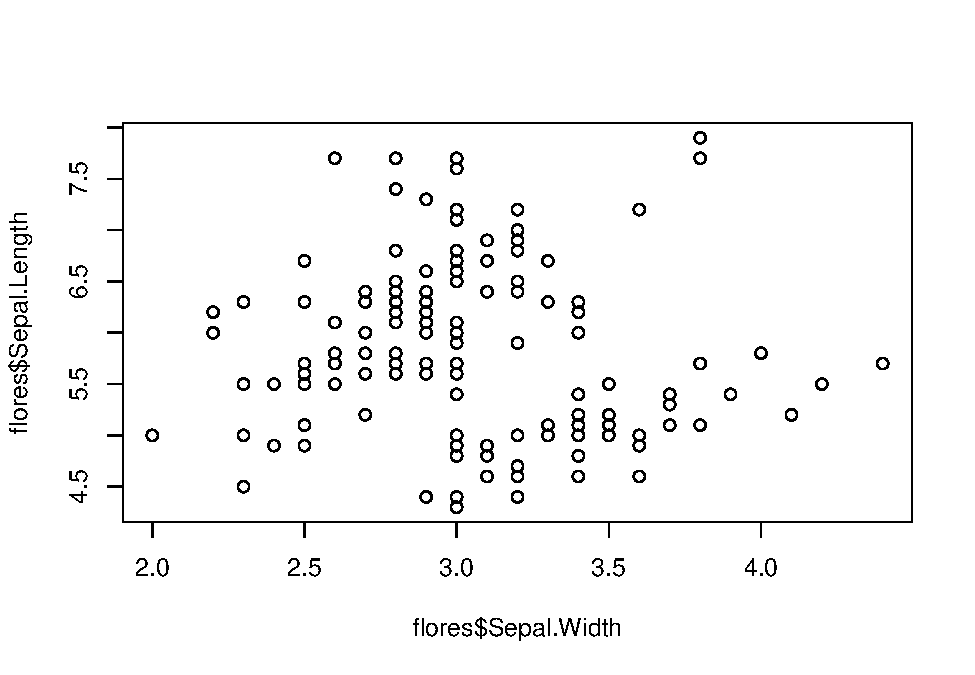
\includegraphics{Esatadistica_en_R_files/figure-latex/unnamed-chunk-136-1.pdf}
Como ven podemos escribir esto realmente en muy pocas palabras. En este caso al escribir \emph{flores\(Sepal.Length ~ flores\)Sepal.Width} le indicamos Length \textbf{en función} de Width, y por eso lo puso en la y. Porque en los gráficos cartesianos y \textbf{es función} de x

Siempre podemos ajustar algunos parámetros de esta función para hacer ``más lindo'' al gráfico. Veamos algunas en un simple ejemplo.

Veamos algunos ajustes:

\begin{itemize}
\item
  El parametro \emph{main}: para poner el título
\item
  Los parámetros \emph{xlab} e \emph{ylab}: permiten cambiar los títulos de los ejes
\item
  pch sirve para seleccionar el tipo de símbolo de punto
\end{itemize}

\begin{Shaded}
\begin{Highlighting}[]
\FunctionTok{plot}\NormalTok{(flores}\SpecialCharTok{$}\NormalTok{Sepal.Length }\SpecialCharTok{\textasciitilde{}}\NormalTok{ flores}\SpecialCharTok{$}\NormalTok{Sepal.Width, }\AttributeTok{main=}\StringTok{"Ratio Sepal/Length"}\NormalTok{, }\AttributeTok{xlab=}\StringTok{"Width"}\NormalTok{, }\AttributeTok{ylab=}\StringTok{"Length"}\NormalTok{, }\AttributeTok{pch=}\StringTok{"*"}\NormalTok{)}
\end{Highlighting}
\end{Shaded}

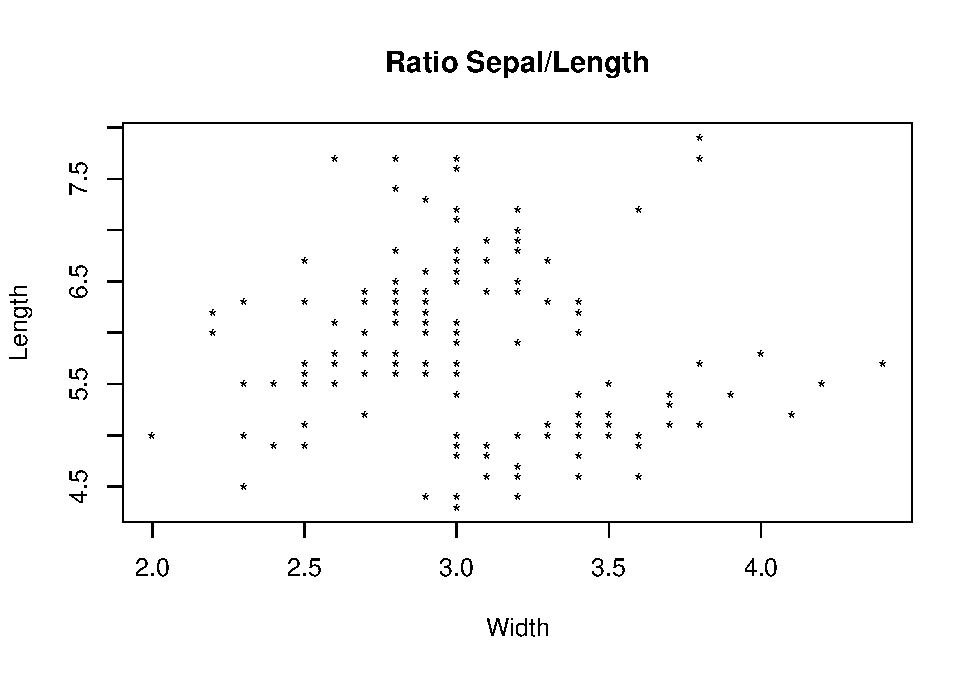
\includegraphics{Esatadistica_en_R_files/figure-latex/unnamed-chunk-137-1.pdf}
Veamos algunos parámetros más:

\begin{itemize}
\item
  El parámetro \emph{cex}: permite cambiar el tamaño del punto
\item
  El parametro \emph{col}: permite crear una paleta
\item
  Una variable entre corchetes después de \emph{col} permite asignarle los colores a las variable
\end{itemize}

\begin{Shaded}
\begin{Highlighting}[]
\FunctionTok{plot}\NormalTok{(flores}\SpecialCharTok{$}\NormalTok{Sepal.Length }\SpecialCharTok{\textasciitilde{}}\NormalTok{ flores}\SpecialCharTok{$}\NormalTok{Sepal.Width, }\AttributeTok{main=}\StringTok{"Ratio Sepal/Length"}\NormalTok{, }\AttributeTok{xlab=}\StringTok{"Width"}\NormalTok{, }\AttributeTok{ylab=}\StringTok{"Length"}\NormalTok{, }\AttributeTok{pch=}\StringTok{"*"}\NormalTok{, }\AttributeTok{cex=}\DecValTok{2}\NormalTok{,}\AttributeTok{col=}\FunctionTok{c}\NormalTok{(}\StringTok{"blue"}\NormalTok{, }\StringTok{"green"}\NormalTok{, }\StringTok{"red"}\NormalTok{)[flores}\SpecialCharTok{$}\NormalTok{Species])}
\end{Highlighting}
\end{Shaded}

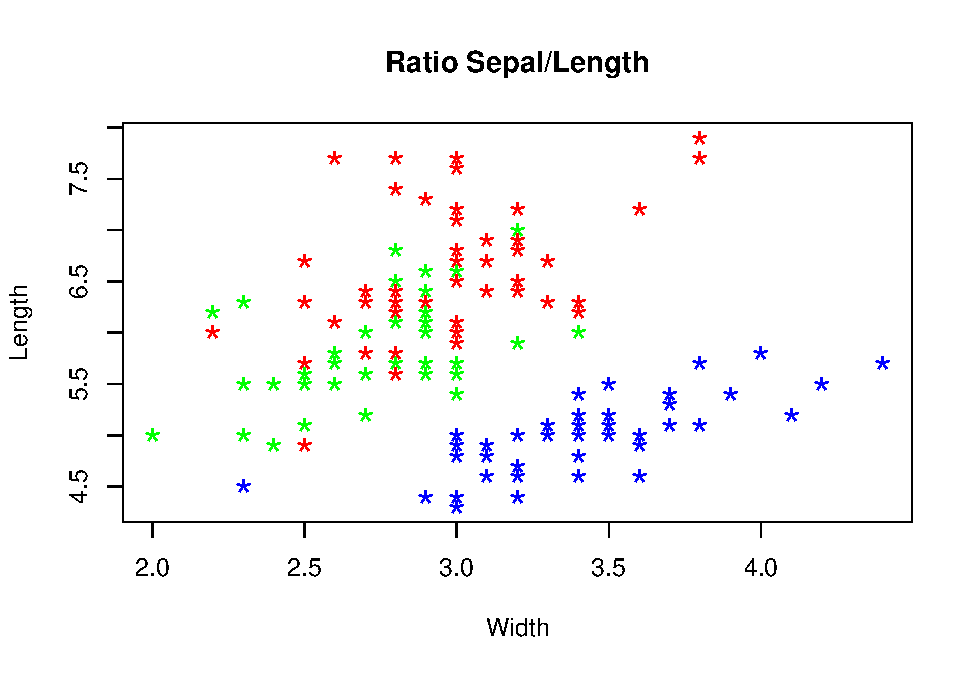
\includegraphics{Esatadistica_en_R_files/figure-latex/unnamed-chunk-138-1.pdf}

\begin{quote}
\textbf{Aclaración}: si bien se puede ``tunear'' estos gráficos, no conviene. Es un proceso engorroso con malos resultados. Tenemos otro paquete para producir gráficos ``para publicar''. Estos gráficos no estan pensados para ser lindos, sino rápidos. Si perdemos tiempo no sirve
\end{quote}

\hypertarget{histograma-y-boxplot}{%
\subsection{Histograma y boxplot}\label{histograma-y-boxplot}}

Muchas de las características de los histogramas y los diagramas de caja las vimos en el capítulo anterior (en la sección de parametricidad), así que abordaremos esto en forma muy sencilla

\begin{Shaded}
\begin{Highlighting}[]
\FunctionTok{hist}\NormalTok{(flores}\SpecialCharTok{$}\NormalTok{Sepal.Width, }
 \AttributeTok{prob =} \ConstantTok{TRUE}\NormalTok{)}
\FunctionTok{lines}\NormalTok{(}\FunctionTok{density}\NormalTok{(flores}\SpecialCharTok{$}\NormalTok{Sepal.Width)) }\DocumentationTok{\#\#Acá vemos como funciona el multilínea}
\end{Highlighting}
\end{Shaded}

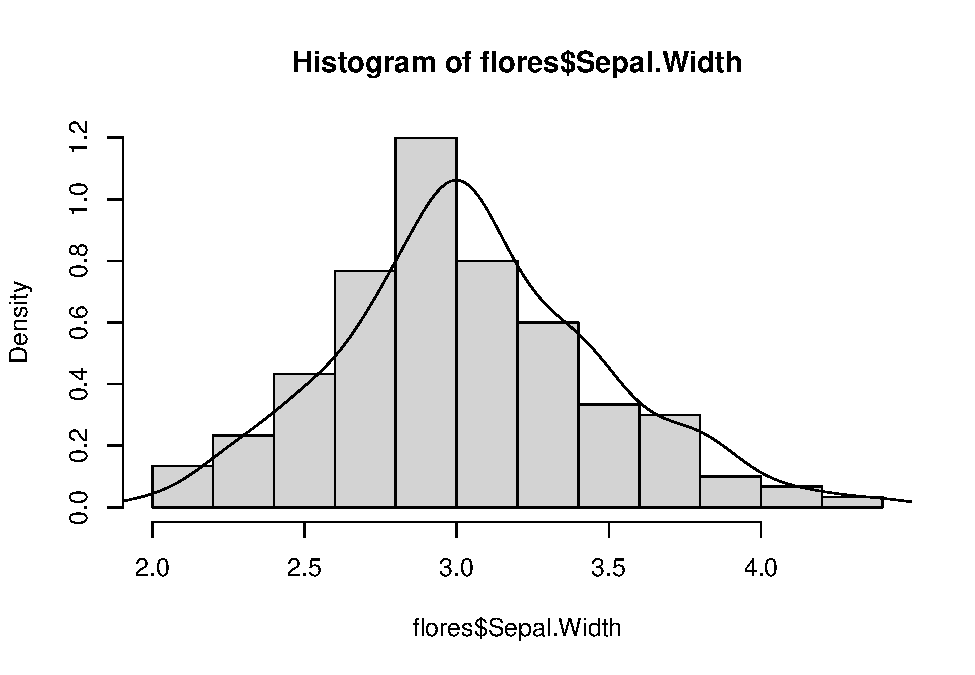
\includegraphics{Esatadistica_en_R_files/figure-latex/unnamed-chunk-139-1.pdf}
En el caso de boxplot podemos graficar una sola variable (como vimos en el capítulo anterior)

\begin{Shaded}
\begin{Highlighting}[]
\FunctionTok{boxplot}\NormalTok{(flores}\SpecialCharTok{$}\NormalTok{Sepal.Width)}
\end{Highlighting}
\end{Shaded}

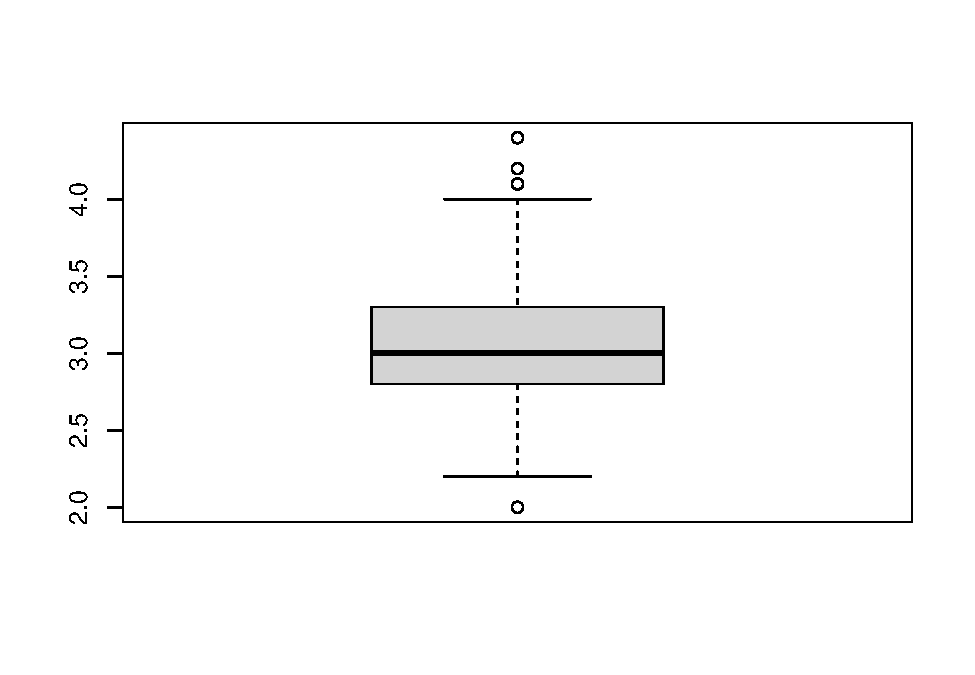
\includegraphics{Esatadistica_en_R_files/figure-latex/unnamed-chunk-140-1.pdf}

O dividirlo por una categórica en grupos

\begin{Shaded}
\begin{Highlighting}[]
\FunctionTok{boxplot}\NormalTok{(flores}\SpecialCharTok{$}\NormalTok{Sepal.Width}\SpecialCharTok{\textasciitilde{}}\NormalTok{flores}\SpecialCharTok{$}\NormalTok{Species)}
\end{Highlighting}
\end{Shaded}

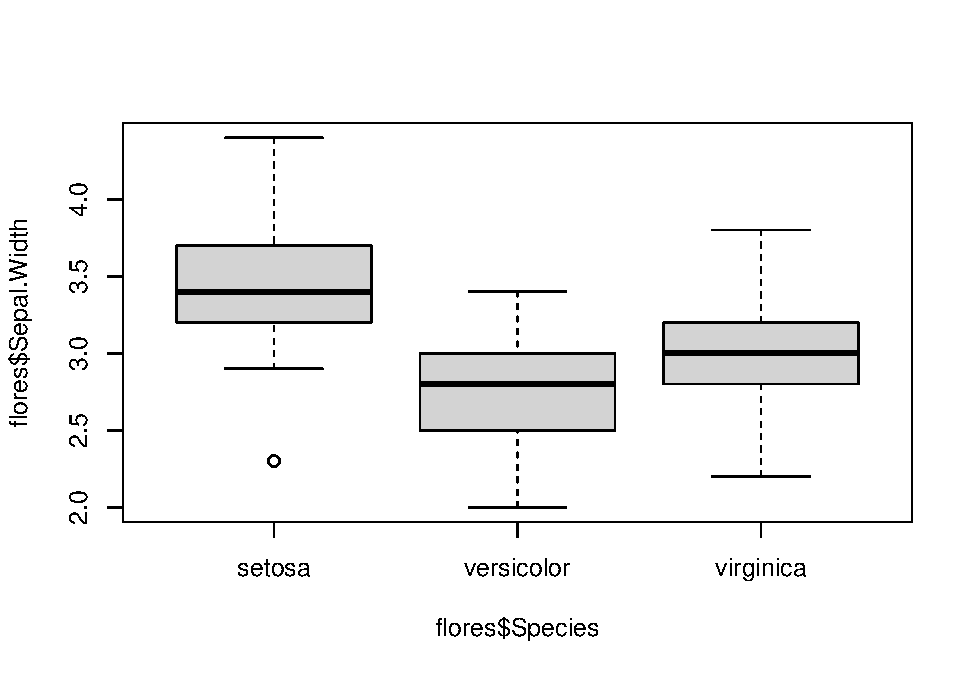
\includegraphics{Esatadistica_en_R_files/figure-latex/unnamed-chunk-141-1.pdf}
De nuevo aquí usamos la virguilla para pedirle que grafique en función de qué.

Estos gráficos son muy útiles para explorar por ejemplo la normalidad y seguir trabajando

\hypertarget{ggplot2}{%
\section{Ggplot2}\label{ggplot2}}

Este paquete es uno de los más utilizados de R. Uno de los aspectos más remarcables es que este paquete plantea una \emph{sintaxis} particular que es reproducida por muchos otros paquetes.

Hay dos grandes sistemas de sintaxis que son muy útiles de aprender, la \emph{sintaxis dplyr} para manipular variables y la \emph{sintaxis ggplot} para hacer gráficos

Veamos en que consiste esta sintaxis ggplot

\hypertarget{sintaxis-ggplot}{%
\subsection{Sintaxis ggplot}\label{sintaxis-ggplot}}

La sintaxis ggplot se resume en 4 aspectos escenciales:

\begin{itemize}
\item
  Una estructura de \textbf{mapeo estético} en donde le decimos a R, donde estan los datos y donde ponerlos (que va en el eje de las x, en el eje de las y, que variable es el color)
\item
  Una \textbf{geometría} que define el tipo de gráfico a utilizar
\item
  Múltiples \textbf{funciones de ajustes} para controlar titulos, paletas de colores, estilos de la grilla, etc.
\item
  Un \textbf{sistema de capas}, que permite superponer distintas geometrías en el orden que deseemos
\end{itemize}

Veamos como funciona en esta sintaxis de un boxplot

\begin{Shaded}
\begin{Highlighting}[]
\FunctionTok{library}\NormalTok{(ggplot2)}

\FunctionTok{ggplot}\NormalTok{(flores, }\FunctionTok{aes}\NormalTok{(}\AttributeTok{y=}\NormalTok{Sepal.Width, }\AttributeTok{x=}\NormalTok{Species, }\AttributeTok{fill=}\NormalTok{Species))}\SpecialCharTok{+}
  \FunctionTok{geom\_boxplot}\NormalTok{()}
\end{Highlighting}
\end{Shaded}

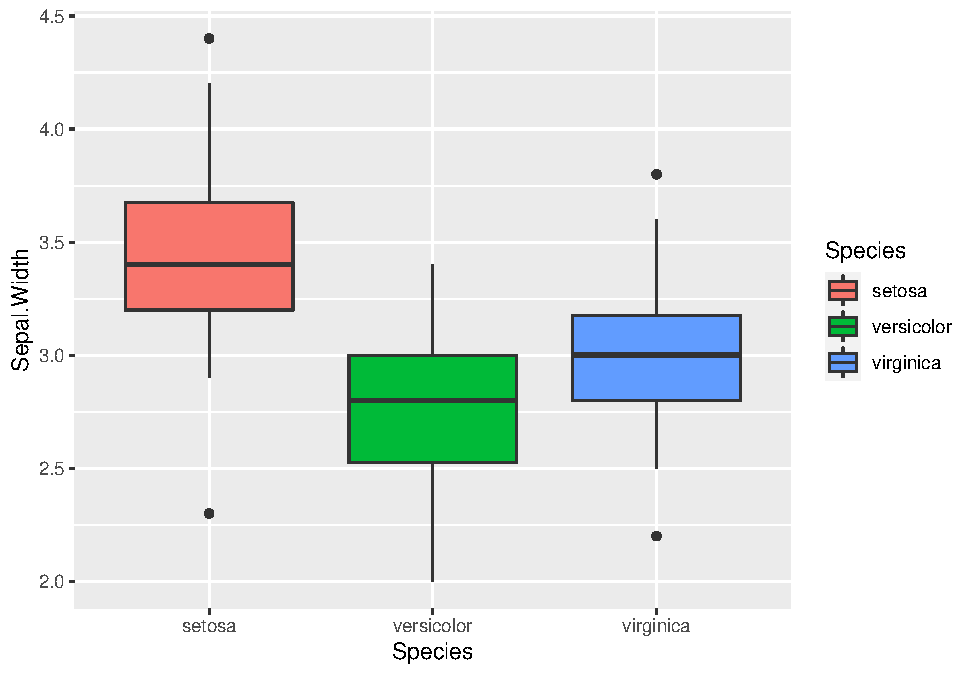
\includegraphics{Esatadistica_en_R_files/figure-latex/unnamed-chunk-142-1.pdf}

Analicemos lo que escribimos con la idea mental de los componentes de la sintaxis:

En la primera línea nos encontramos con esto:

\begin{quote}
ggplot(flores, aes(y=Sepal.Width, x=Species, fill=Species))+
\end{quote}

Esta estructura es el \textbf{mapeo estético}:

\begin{itemize}
\item
  El primer argumento es de donde surgen los datos (el dataset)
\item
  El segundo argumento es la estética, aquí: 1) Asignamos la variable a y 2) Asignamos la variable a x 3) y asignamos la variable al color
\item
  esta línea debe terminar con un \textbf{+}, esto le dice a R que hay una línea siguiente (una capa más)
\end{itemize}

La segunda línea es:

\begin{quote}
geom\_boxplot()
\end{quote}

que asigna que geometría le vamos a pedir

\hypertarget{recapitulemos}{%
\subsubsection{Recapitulemos}\label{recapitulemos}}

Vimos que para crear un boxplor en R básico debo escribir esto:

\begin{quote}
boxplot(Sepal.Width \textasciitilde{} Species)
\end{quote}

y para hacerlo en ggplot:

\begin{quote}
\_ggplot(flores, aes(y=Sepal.Width, x=Species, fill=Species))+
geom\_boxplot()
\end{quote}

¿Qué sentido tiene utilizar una función más compleja para obtener el mismo gráfico? La respuesta corta es niguno. La respuesta larga es otra pregunta: ¿para qué queremos el gráfico?. Si queremos un gráfico para ver como son los datos, no es ggplot lo que necesitamos. En las secciones que siguen vamos a ver como ggplot nos sirve para crear ``el gráfico'' para publicar.

\hypertarget{el-mapeo-estuxe9tico}{%
\subsection{El mapeo estético}\label{el-mapeo-estuxe9tico}}

El mapeo estético como habíamos visto en la sección anterior es asignar una variable a una característica visual del gráfico, las posibilidades:

\begin{itemize}
\item
  asignar un valor a la posicion en el eje x o en el y
\item
  asignar una variable al color (color)
\item
  asignar una variable al relleno de geometrías sólidas (fill)
\item
  asignar una variable a un tipo de forma (shape)
\item
  asignar una variable a un tamaño (size)
\end{itemize}

\textbf{\emph{Importante}}

El mapeo estético \textbf{necesita} que todas nuestras variables tengan su correcta \textbf{definición de clase} Esta es la principal fuente de error en los gráficos ggplot

Veamos algunos ejemplos de mapeos esteticos en un \emph{gráfico de dispersión}

\begin{Shaded}
\begin{Highlighting}[]
\FunctionTok{ggplot}\NormalTok{(flores, }\FunctionTok{aes}\NormalTok{(}\AttributeTok{x=}\NormalTok{Sepal.Length, }\AttributeTok{y=}\NormalTok{Sepal.Width, }\AttributeTok{color=}\NormalTok{Species))}\SpecialCharTok{+}
  \FunctionTok{geom\_point}\NormalTok{()}
\end{Highlighting}
\end{Shaded}

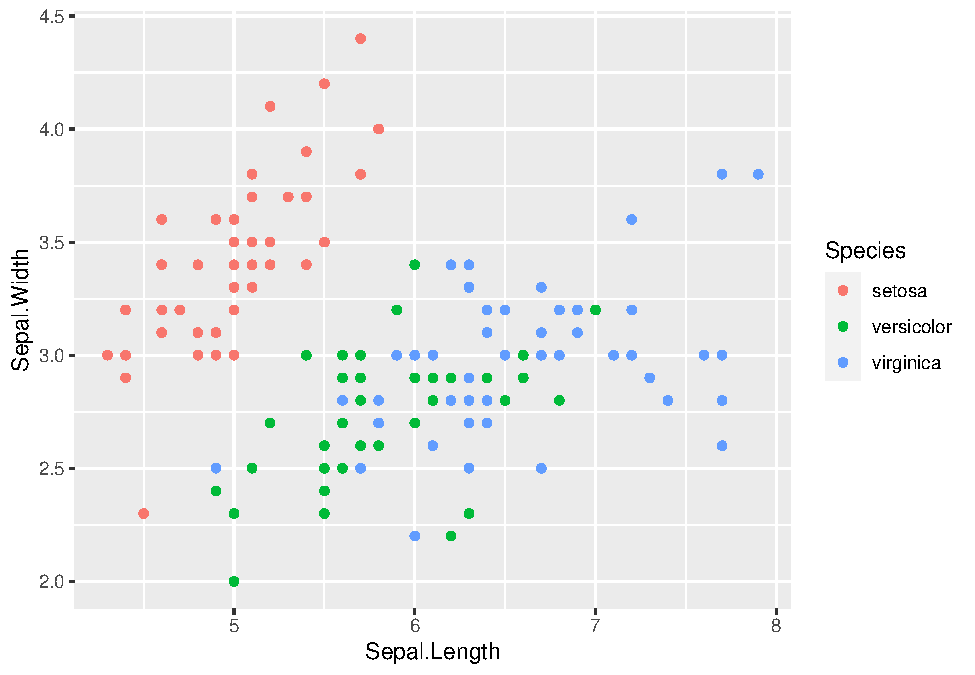
\includegraphics{Esatadistica_en_R_files/figure-latex/unnamed-chunk-143-1.pdf}

Dentro del mapeo entonces: 1) asignamos el largo a la ``x'' 2) el ancho a las ``y'' y 3) la especie al color

\begin{Shaded}
\begin{Highlighting}[]
\FunctionTok{ggplot}\NormalTok{(flores, }\FunctionTok{aes}\NormalTok{(}\AttributeTok{x=}\NormalTok{Sepal.Length, }\AttributeTok{y=}\NormalTok{Sepal.Width, }\AttributeTok{shape=}\NormalTok{Species))}\SpecialCharTok{+}
  \FunctionTok{geom\_point}\NormalTok{()}
\end{Highlighting}
\end{Shaded}

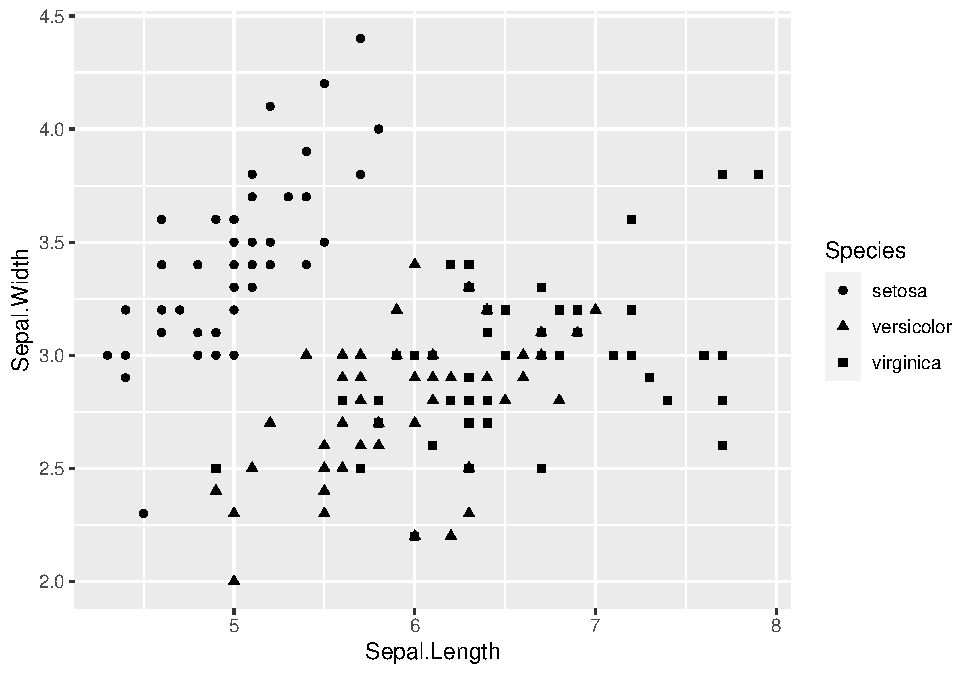
\includegraphics{Esatadistica_en_R_files/figure-latex/unnamed-chunk-144-1.pdf}
Dentro del mapeo entonces: 1) asignamos el largo a la ``x'' 2) el ancho a las ``y'' y 3) la especie al tipo de forma de punto.

Incluso podemos asignar varios atributos esteticos a la misma variable, como aquí:

\begin{Shaded}
\begin{Highlighting}[]
\FunctionTok{ggplot}\NormalTok{(flores, }\FunctionTok{aes}\NormalTok{(}\AttributeTok{x=}\NormalTok{Sepal.Length, }\AttributeTok{y=}\NormalTok{Sepal.Width, }\AttributeTok{color=}\NormalTok{Species, }\AttributeTok{shape=}\NormalTok{Species))}\SpecialCharTok{+}
  \FunctionTok{geom\_point}\NormalTok{()}
\end{Highlighting}
\end{Shaded}

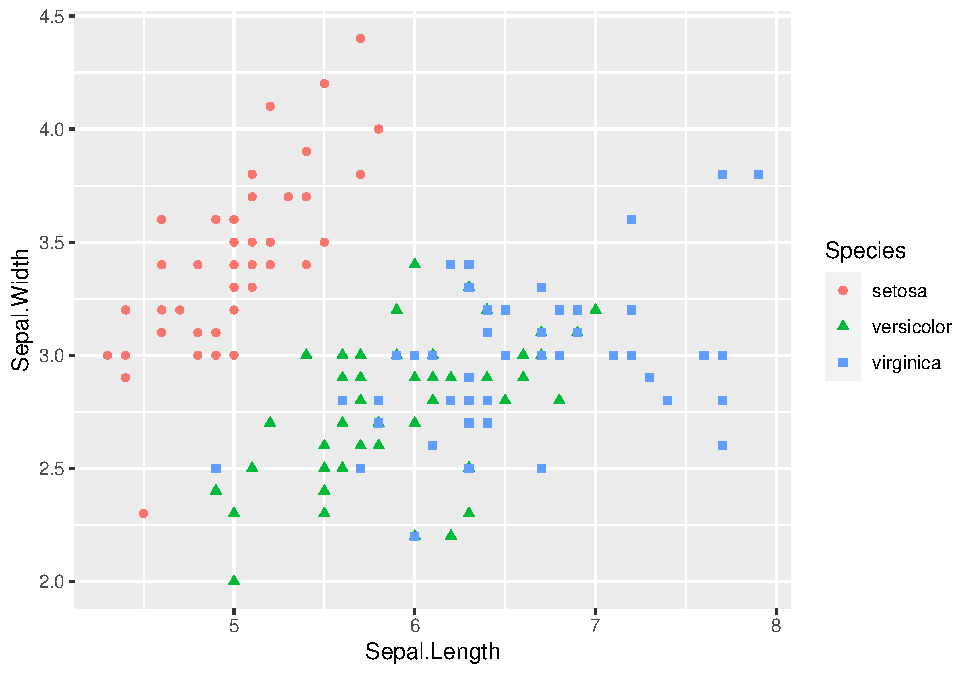
\includegraphics{Esatadistica_en_R_files/figure-latex/unnamed-chunk-145-1.pdf}

En este caso : 1) asignamos el largo a la ``x'' 2) el ancho a las ``y'' 3) la especie al tipo de forma de punto y 4) el color a la especie

Veamos que pasa si en lugar de una variable categórica como atributo del color ponemos una continua

\begin{Shaded}
\begin{Highlighting}[]
\FunctionTok{ggplot}\NormalTok{(flores, }\FunctionTok{aes}\NormalTok{(}\AttributeTok{x=}\NormalTok{Sepal.Length, }\AttributeTok{y=}\NormalTok{Sepal.Width, }\AttributeTok{color=}\NormalTok{Petal.Width))}\SpecialCharTok{+}
  \FunctionTok{geom\_point}\NormalTok{()}
\end{Highlighting}
\end{Shaded}

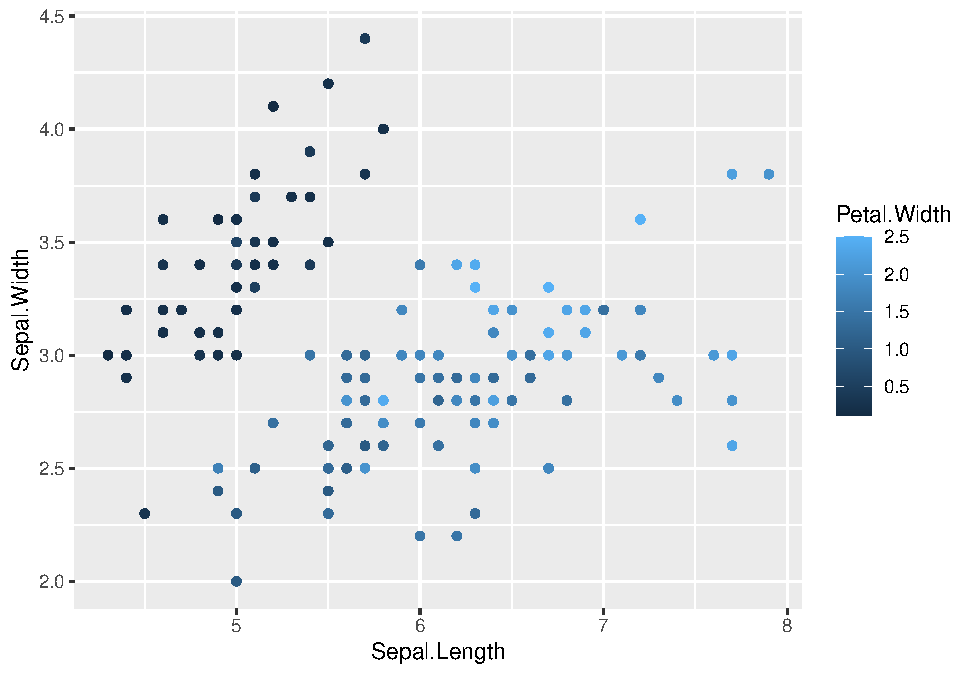
\includegraphics{Esatadistica_en_R_files/figure-latex/unnamed-chunk-146-1.pdf}

En este caso, asignamos una variable que R sabe es una continua a un color. Al graficar una continua R sabe que los valores no son bloques independientes entre sí (como en una paleta de colores) sino que hay infinitos valores entre uno y otro. para graficar este suceso recurre a mostrar una graduación de un sólo color, un proceso que se conoce como \textbf{escalar} la variable (porque la puso en una escala de azules). Para que ocurra esto es muy, muy, muy importante que las variables tengan asignada la clase que les corresponde.

Veamos que pasa si le ``pifeamos'' en eso:

\begin{Shaded}
\begin{Highlighting}[]
\NormalTok{flores}\SpecialCharTok{$}\NormalTok{Petal.Width}\OtherTok{\textless{}{-}}\FunctionTok{as.factor}\NormalTok{(flores}\SpecialCharTok{$}\NormalTok{Petal.Width) }\CommentTok{\# esta linea es para definir mal el tipo de variable (un error, a propósito)}

\FunctionTok{ggplot}\NormalTok{(flores, }\FunctionTok{aes}\NormalTok{(}\AttributeTok{x=}\NormalTok{Sepal.Length, }\AttributeTok{y=}\NormalTok{Sepal.Width, }\AttributeTok{color=}\NormalTok{Petal.Width))}\SpecialCharTok{+}
  \FunctionTok{geom\_point}\NormalTok{()}
\end{Highlighting}
\end{Shaded}

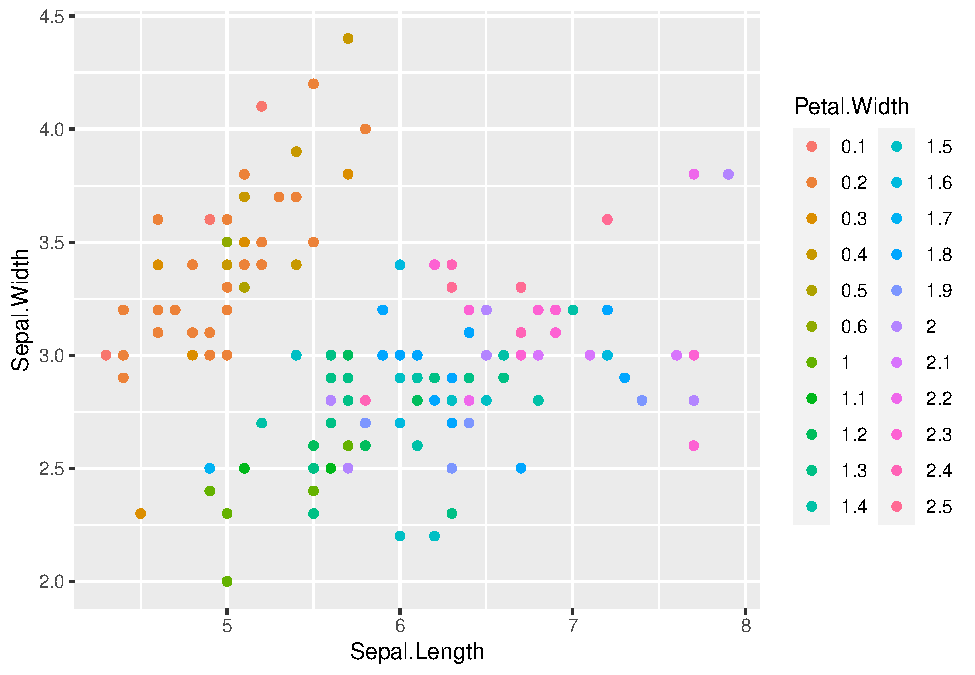
\includegraphics{Esatadistica_en_R_files/figure-latex/unnamed-chunk-147-1.pdf}

\begin{Shaded}
\begin{Highlighting}[]
\NormalTok{flores}\SpecialCharTok{$}\NormalTok{Petal.Width}\OtherTok{\textless{}{-}}\FunctionTok{as.numeric}\NormalTok{(flores}\SpecialCharTok{$}\NormalTok{Petal.Width) }\CommentTok{\# para reparar el error y seguir trabajando}
\end{Highlighting}
\end{Shaded}

Creamos un desastre en donde asigno un color independiente a cada valor que adoptó la variable (esto puede llevar a crear miles de colores así que mucho cuidado)

\hypertarget{las-geometruxedas}{%
\subsection{Las geometrías}\label{las-geometruxedas}}

Después de la definición de las variables a sus condiciones (la que llamamos anteriormente \emph{mapeo estético}) debemos indicarle el tipo de gráfico que queremos que sea creado, estos gráficos se denominan geometrías y son básicamente los siguientes:

\begin{itemize}
\item
  \textbf{geom\_point()} produce un gráfico de dispersión o \emph{scatter plot}
\item
  \textbf{geom\_boxplot()} produce un gráfico de caja y bigotes (o \_box-p) para resumir la distribución de un conjunto de puntos.
\item
  \textbf{geom\_histogram()} y \textbf{geom\_freqpoly()} sirven àra crear gráficos de frecuencia e histogramas, resumen la distribución de variables continuas.
\item
  \textbf{geom\_bar()} crea gráficos de barra utilizadps para resumir la distribución de las variables categóricas.
\item
  \textbf{geom\_path()} y \textbf{geom\_line()} dibujan líneas entre los puntos de datos. Un gráfico de líneas está limitado a producir líneas que van de izquierda a derecha, mientras que los caminos ( \emph{geom\_path}) pueden ir en cualquier dirección. Las líneas se utilizan normalmente para explorar cómo cambian las cosas con el tiempo.
\item
  \textbf{geom\_smooth()}: ajusta una línea a los datos y muestra tanto el ajuste como su error estándar (en términos de un intervalo de confianza).
\end{itemize}

\hypertarget{capas}{%
\subsection{Capas}\label{capas}}

Una de las cosas más interesantes con respecto a ggplot es que es posible \emph{apilar geometrías} e incluso modificar la estética de cada una, veamoslo con un ejemplo:

Vamos a crear un gráfico de dispersión como el anterior

\begin{Shaded}
\begin{Highlighting}[]
\FunctionTok{ggplot}\NormalTok{(flores, }\FunctionTok{aes}\NormalTok{(}\AttributeTok{x=}\NormalTok{Sepal.Length, }\AttributeTok{y=}\NormalTok{Sepal.Width))}\SpecialCharTok{+}
  \FunctionTok{geom\_point}\NormalTok{()}
\end{Highlighting}
\end{Shaded}

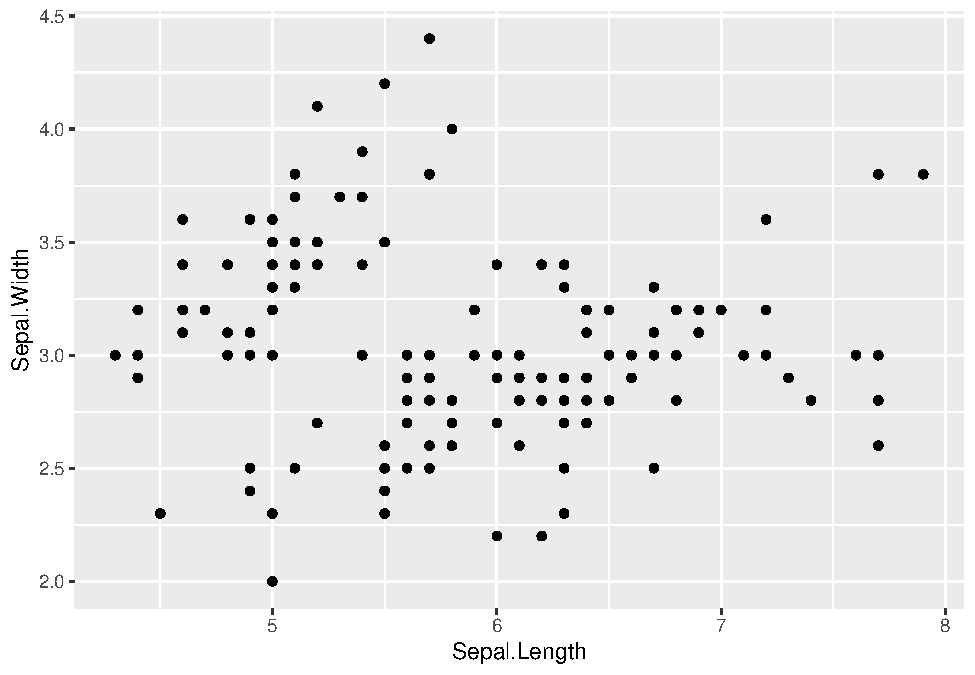
\includegraphics{Esatadistica_en_R_files/figure-latex/unnamed-chunk-148-1.pdf}

Imaginemos que queremos producir una línea que implique un ajuste ``lineal'' a estos datos, deberíamos \emph{apilar} otra geometría

\begin{Shaded}
\begin{Highlighting}[]
\FunctionTok{ggplot}\NormalTok{(flores, }\FunctionTok{aes}\NormalTok{(}\AttributeTok{x=}\NormalTok{Sepal.Length, }\AttributeTok{y=}\NormalTok{Sepal.Width))}\SpecialCharTok{+}
  \FunctionTok{geom\_point}\NormalTok{()}\SpecialCharTok{+}
  \FunctionTok{geom\_smooth}\NormalTok{(}\AttributeTok{method =} \StringTok{"lm"}\NormalTok{) }\CommentTok{\#este parámetro es para que el método de ajuste sea lineal}
\end{Highlighting}
\end{Shaded}

\begin{verbatim}
## `geom_smooth()` using formula 'y ~ x'
\end{verbatim}

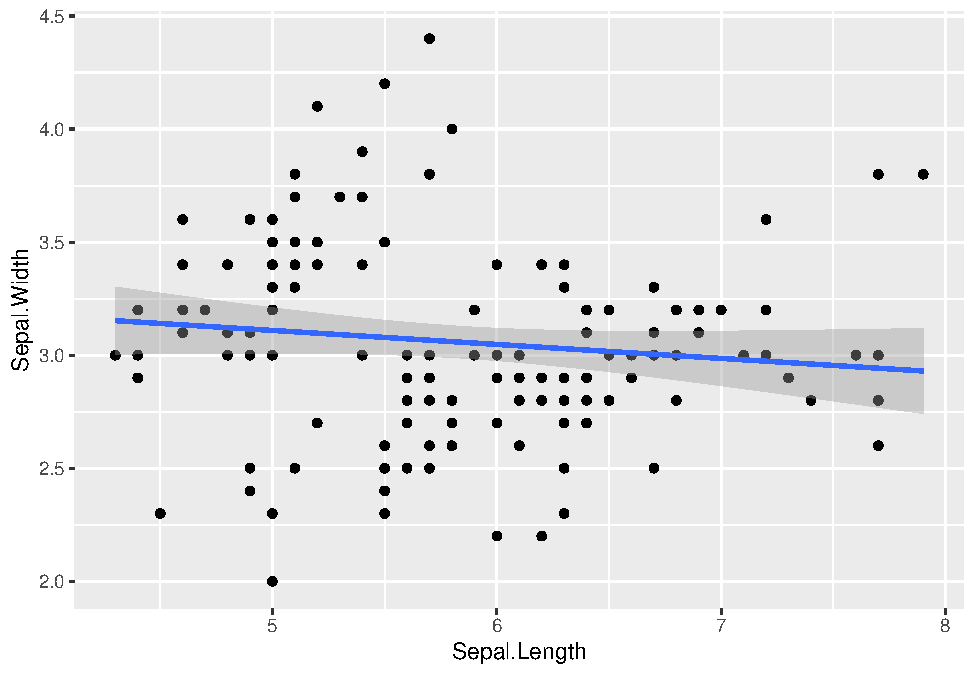
\includegraphics{Esatadistica_en_R_files/figure-latex/unnamed-chunk-149-1.pdf}
Veamos ahora dos gráficos y sus diferencias:

El primero:

\begin{Shaded}
\begin{Highlighting}[]
\FunctionTok{ggplot}\NormalTok{(flores, }\FunctionTok{aes}\NormalTok{(}\AttributeTok{x=}\NormalTok{Sepal.Length, }\AttributeTok{y=}\NormalTok{Sepal.Width, }\AttributeTok{color=}\NormalTok{Species))}\SpecialCharTok{+}
  \FunctionTok{geom\_point}\NormalTok{()}\SpecialCharTok{+}
  \FunctionTok{geom\_smooth}\NormalTok{(}\AttributeTok{method =} \StringTok{"lm"}\NormalTok{) }\CommentTok{\#este parámetro es para que el método de ajuste sea lineal}
\end{Highlighting}
\end{Shaded}

\begin{verbatim}
## `geom_smooth()` using formula 'y ~ x'
\end{verbatim}

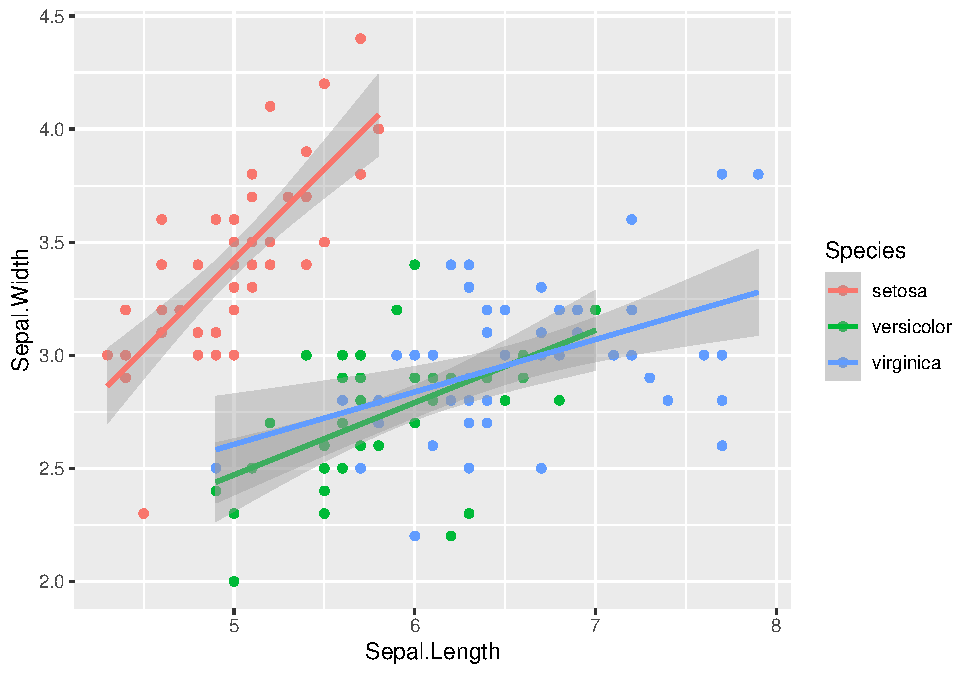
\includegraphics{Esatadistica_en_R_files/figure-latex/unnamed-chunk-150-1.pdf}
El segundo:

\begin{Shaded}
\begin{Highlighting}[]
\FunctionTok{ggplot}\NormalTok{(flores, }\FunctionTok{aes}\NormalTok{(}\AttributeTok{x=}\NormalTok{Sepal.Length, }\AttributeTok{y=}\NormalTok{Sepal.Width))}\SpecialCharTok{+}
  \FunctionTok{geom\_point}\NormalTok{(}\FunctionTok{aes}\NormalTok{(}\AttributeTok{color=}\NormalTok{Species))}\SpecialCharTok{+}
  \FunctionTok{geom\_smooth}\NormalTok{(}\AttributeTok{method =} \StringTok{"lm"}\NormalTok{) }\CommentTok{\#este parámetro es para que el método de ajuste sea lineal}
\end{Highlighting}
\end{Shaded}

\begin{verbatim}
## `geom_smooth()` using formula 'y ~ x'
\end{verbatim}

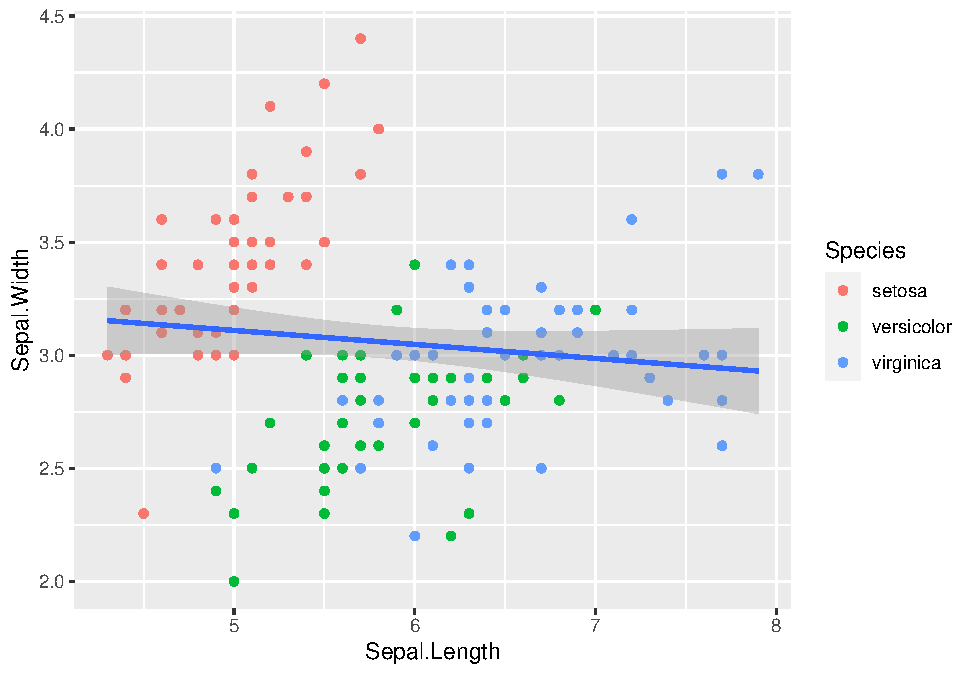
\includegraphics{Esatadistica_en_R_files/figure-latex/unnamed-chunk-151-1.pdf}

¿Por qué son diferentes?:

Prestemos mucha atención al mapeo estético, en el primero: el color está asignado junto con la estética \textbf{global} del gráfico (en la primera línea), mientras que en el segundo el mapeo estético está como un argumento de \emph{geom\_point} afectando sólo a esa capa.

Algunos conceptos importantes con respecto al trabajo de capas:

\begin{enumerate}
\def\labelenumi{\arabic{enumi}.}
\item
  El mapeo estético puede afectar a una o más capas depende en donde decidamos incorporarlo
\item
  El orden de las líneas determina el orden en que se superponen, miremos estos dos gráficos:
\end{enumerate}

\begin{Shaded}
\begin{Highlighting}[]
\FunctionTok{ggplot}\NormalTok{(flores, }\FunctionTok{aes}\NormalTok{(}\AttributeTok{y=}\NormalTok{Sepal.Width, }\AttributeTok{x=}\NormalTok{Species, }\AttributeTok{fill=}\NormalTok{Species))}\SpecialCharTok{+}
  \FunctionTok{geom\_boxplot}\NormalTok{()}\SpecialCharTok{+}
  \FunctionTok{geom\_point}\NormalTok{()}
\end{Highlighting}
\end{Shaded}

\includegraphics{Esatadistica_en_R_files/figure-latex/unnamed-chunk-152-1.pdf}

\begin{Shaded}
\begin{Highlighting}[]
\FunctionTok{ggplot}\NormalTok{(flores, }\FunctionTok{aes}\NormalTok{(}\AttributeTok{y=}\NormalTok{Sepal.Width, }\AttributeTok{x=}\NormalTok{Species, }\AttributeTok{fill=}\NormalTok{Species))}\SpecialCharTok{+}
  \FunctionTok{geom\_point}\NormalTok{()}\SpecialCharTok{+}
  \FunctionTok{geom\_boxplot}\NormalTok{()}
\end{Highlighting}
\end{Shaded}

\includegraphics{Esatadistica_en_R_files/figure-latex/unnamed-chunk-153-1.pdf}

Un gráfico \emph{cubre} al otro en el sentido en que las capas se superponen, tener siempre en cuenta esto a la hora de graficar.

\hypertarget{ejercicios-4}{%
\section{\texorpdfstring{ Ejercicios:}{ Ejercicios:}}\label{ejercicios-4}}

Para estos ejercicios vamos a trabajar con otro dataset ``ChickWeight'', incluído en un paquete que se llama ``datasets''.

``ChickWeight'' es una base de datos con 578 registros sobre el efecto de 4 tipos de dietas distintas (la variable ``Diet'') sobre el peso (``weigth'') de pollitos de distintas edades, reportadas en días (la variable ``Time'')

Nuestro ejercicio consiste en:

\begin{enumerate}
\def\labelenumi{\arabic{enumi}.}
\item
  Instalar el paquete ``datasets'' (si no lo han hecho ya)
\item
  Activar el paquete
\item
  Asignar la base de datos ``cars'' al objeto data
\end{enumerate}

Y realizar los siguientes gráficos:

\begin{enumerate}
\def\labelenumi{\arabic{enumi}.}
\setcounter{enumi}{3}
\item
  Un gráfico rápido mostrando el peso de los pollitos en función de su edad
\item
  Un gráfico de cajas con el peso de los pollitos por dietas (rápido o no, ustedes deciden)
\item
  Un gráfico de dispersión con el peso y la edad de los pollitos, coloreados por dieta
\item
  Un gráfico de dispersión con el peso y la edad de los pollitos, coloreados por dieta, con una línea de ajuste lineal por cada dieta
\item
  Un gráfico de dispersión con el peso y la edad de los pollitos, coloreados por dieta, con una línea de ajuste lineal para todos los pollitos en común
\end{enumerate}

A trabajar

\hypertarget{respuestas-2}{%
\section{\texorpdfstring{ Respuestas:}{ Respuestas:}}\label{respuestas-2}}

Si son tan vagos de haber llegado a está sección sin hacer por su propia mano los ejercicios, acá están las respuestas pero recuerden ``NO PAIN NO GAIN''

\begin{Shaded}
\begin{Highlighting}[]
\CommentTok{\# los puntos 1 a 3}
\FunctionTok{library}\NormalTok{(datasets)}

\NormalTok{data}\OtherTok{\textless{}{-}}\NormalTok{ChickWeight}

\CommentTok{\# Un gráfico rápido mostrando el peso de los pollitos en función de su edad}

\FunctionTok{plot}\NormalTok{(data}\SpecialCharTok{$}\NormalTok{weight}\SpecialCharTok{\textasciitilde{}}\NormalTok{data}\SpecialCharTok{$}\NormalTok{Time)}
\end{Highlighting}
\end{Shaded}

\includegraphics{Esatadistica_en_R_files/figure-latex/unnamed-chunk-154-1.pdf}

\begin{Shaded}
\begin{Highlighting}[]
\CommentTok{\# Un gráfico de cajas con el peso de los pollitos por dietas (yo decidí un ggplot porque estoy obsesionado con el pero quizás un gráfico rápido hubiera sido mejor)}

\FunctionTok{library}\NormalTok{(ggplot2)}
\FunctionTok{ggplot}\NormalTok{(data, }\FunctionTok{aes}\NormalTok{(}\AttributeTok{X=}\NormalTok{Diet, }\AttributeTok{y=}\NormalTok{weight))}\SpecialCharTok{+}
  \FunctionTok{geom\_boxplot}\NormalTok{()}
\end{Highlighting}
\end{Shaded}

\includegraphics{Esatadistica_en_R_files/figure-latex/unnamed-chunk-154-2.pdf}

\begin{Shaded}
\begin{Highlighting}[]
\CommentTok{\# Un gráfico de dispersión con el peso y la edad de los pollitos, coloreados por dieta}
\FunctionTok{ggplot}\NormalTok{(data, }\FunctionTok{aes}\NormalTok{(}\AttributeTok{x=}\NormalTok{Time, }\AttributeTok{y=}\NormalTok{weight, }\AttributeTok{color=}\NormalTok{Diet))}\SpecialCharTok{+}
  \FunctionTok{geom\_point}\NormalTok{()}
\end{Highlighting}
\end{Shaded}

\includegraphics{Esatadistica_en_R_files/figure-latex/unnamed-chunk-154-3.pdf}

\begin{Shaded}
\begin{Highlighting}[]
\CommentTok{\# Un gráfico de dispersión con el peso y la edad de los pollitos, coloreados por dieta, con una línea de ajuste lineal por cada dieta}
\FunctionTok{ggplot}\NormalTok{(data, }\FunctionTok{aes}\NormalTok{(}\AttributeTok{x=}\NormalTok{Time, }\AttributeTok{y=}\NormalTok{weight, }\AttributeTok{color=}\NormalTok{Diet))}\SpecialCharTok{+}
  \FunctionTok{geom\_point}\NormalTok{()}\SpecialCharTok{+}
  \FunctionTok{geom\_smooth}\NormalTok{(}\AttributeTok{method=}\StringTok{"lm"}\NormalTok{)}
\end{Highlighting}
\end{Shaded}

\begin{verbatim}
## `geom_smooth()` using formula 'y ~ x'
\end{verbatim}

\includegraphics{Esatadistica_en_R_files/figure-latex/unnamed-chunk-154-4.pdf}

\begin{Shaded}
\begin{Highlighting}[]
\CommentTok{\#  Un gráfico de dispersión con el peso y la edad de los pollitos, coloreados por dieta, con una línea de ajuste lineal para todos los pollitos en común}
\FunctionTok{ggplot}\NormalTok{(data, }\FunctionTok{aes}\NormalTok{(}\AttributeTok{x=}\NormalTok{Time, }\AttributeTok{y=}\NormalTok{weight))}\SpecialCharTok{+}
  \FunctionTok{geom\_point}\NormalTok{(}\FunctionTok{aes}\NormalTok{(}\AttributeTok{color=}\NormalTok{Diet))}\SpecialCharTok{+}
  \FunctionTok{geom\_smooth}\NormalTok{(}\AttributeTok{method=}\StringTok{"lm"}\NormalTok{)}
\end{Highlighting}
\end{Shaded}

\begin{verbatim}
## `geom_smooth()` using formula 'y ~ x'
\end{verbatim}

\includegraphics{Esatadistica_en_R_files/figure-latex/unnamed-chunk-154-5.pdf}

¿Qué piensan, son las dietas efectivas para subir el peso de los pollitos?, o los pollitos suben de peso sólo por crecer.

Bueno tranquilos que hay que ``testear'' estas hipótesis\ldots{} y vamos a hacerlas en los próximos capítulos

\hypertarget{matriz-de-confusiuxf3n}{%
\chapter{Matriz de confusión}\label{matriz-de-confusiuxf3n}}

En esta sección veremos algunos conceptos sencillos sobre las matrices de confusión. Estas son herramientas para medir la precisión de un test tanto de laboratorio, clínico como estadístico. Los que se dediquen a la medicina y sus afines seguramente estarán habituados a ellos aunque no las conozcan por ese nombre

Una matriz de confusión es una tabla que categorizará las predicciones frente a los valores reales. Incluye dos dimensiones, entre ellas una indicará los valores predichos (el resultado de un test) y otra representará los valores reales.

Cada fila de la matriz de confusión representará los valores predichos y las columnas serán responsables de los valores reales. También puede ser a la inversa. Aunque las matrices son fáciles, la terminología que hay detrás parece compleja.

La matriz de confusión más intuitiva es esta:

\includegraphics[width=11.6in]{img/matrix}

Esta es una matriz de las que llamamos 2x2, es decir contrastamos una variable con dos niveles, con otra con dos niveles. Vamos a despegarnos por un segundo del concepto de salud/enfermedad porque las matrices de confusión sirven para detectar condiciones.
A veces la condición es ``ganar la lotería'' y otras veces es ``tener una metástasis de cerebro'' por ende dejar asociado a cada columna conceptos con valoraciones positivas o negativas no tiene sentido. Generalicemos:

\includegraphics[width=11.6in]{img/matrix2}

Estamos de acuerdo que son matrices de 2x2, pero es importante saber que las matrices pueden tener la dimensión que sea necesaria, podemos usar un test como la glucemia para diagnostica ``normal'', ``prediabetes'' y ``diabetes''. Lo que sí deben tener las matrices de confusión es simetría, es decir la condición real a diagnosticar y el test deben tener los mismos niveles.

Nuestro caso de la glucemia se vería así:

\includegraphics[width=11.38in]{img/matrix3}

\hypertarget{componentes-de-la-matriz-de-confusiuxf3n}{%
\section{Componentes de la matriz de confusión}\label{componentes-de-la-matriz-de-confusiuxf3n}}

Vamos a hablar un poco de la terminología

Como habrán notado en los esquemas hay circulos verdes y x rojas en donde hay discordancia.

Las \emph{discordancias} se llaman \textbf{\emph{falsos}} y las \emph{concordancias} \textbf{\emph{verdaderos}}

La \emph{ocurrencia de la clase de interés} se llama \textbf{\emph{positivo}}, independiente de la valoración del resultado del test (un test de embarazo positivo y un test de cancer positivo, son positivos independiente de la felicidad o la tristeza que da cada uno) \emph{el resto de las clases} serán negativas (esto es muy importante si la variable tiene más de dos niveles, hay que decir cuál es el evento de interés y todos los demás son negativos).

De esta forma, con esto dos conceptos se construyen 4 categorías:

\begin{itemize}
\item
  \textbf{\emph{Verdadero positivo (VP)}} - El test detecta la presencia de la clase de interes y la clasifica correctamente ya que la condición se produce en realidad.
\item
  \textbf{\emph{Verdadero negativo (VN)}} - El test \textbf{\emph{no}} detecta la presencia de la clase de interes y la clasifica correctamente ya que la condición \textbf{\emph{no}} se produce en realidad.
\item
  \textbf{\emph{Falso positivo (FP)}} - El test detecta equivocadamente la aparición del evento de interés pero \textbf{\emph{no}} se ha producido en la realidad
\item
  \textbf{\emph{Falso positivo (FN)}} - El test equivocadamente *\textbf{no} detecta la aparición del evento de interés pero sí se ha producido en la realidad.
\end{itemize}

\hypertarget{anuxe1lisis-de-la-matriz-de-confusiuxf3n}{%
\section{Análisis de la matriz de confusión}\label{anuxe1lisis-de-la-matriz-de-confusiuxf3n}}

Muchos de ustedes estarán familiarizados con los términos que expusimos anteriormente y los que seguirán a continuación, pero siempre vale la pena refrescarlos

\hypertarget{sensibilidad}{%
\subsection{Sensibilidad}\label{sensibilidad}}

Consideremos el ejemplo de una prueba médica para diagnosticar una enfermedad. La sensibilidad se refiere a la capacidad de la prueba para detectar correctamente a los pacientes que padecen la enfermedad. En el ejemplo de una prueba médica utilizada para identificar una enfermedad, la sensibilidad (a veces también denominada \emph{tasa de detección} en un entorno clínico) de la prueba es la proporción de personas que dan positivo en la prueba de la enfermedad entre las que la padecen.

Algo así:

\includegraphics[width=15.35in]{img/sens}

Un resultado negativo en una prueba con alta sensibilidad es útil para descartar la enfermedad. Una prueba de alta sensibilidad es fiable cuando su resultado es negativo, ya que rara vez diagnostica mal a quienes tienen la enfermedad. Una prueba con una sensibilidad del 100\% reconocerá a todos los pacientes con la enfermedad al dar un resultado positivo. Un resultado negativo de la prueba descartaría definitivamente la presencia de la enfermedad en un paciente. Sin embargo, un resultado positivo en una prueba con alta sensibilidad no es necesariamente útil para descartar la enfermedad. Supongamos que un kit de pruebas ``falso'' está diseñado para dar siempre un resultado positivo. Cuando se utiliza en pacientes enfermos, todos los pacientes dan un resultado positivo, lo que da a la prueba una sensibilidad del 100\%. Sin embargo, la sensibilidad no tiene en cuenta los falsos positivos. La prueba falsa también da un resultado positivo en todos los pacientes sanos, lo que le confiere una tasa de falsos positivos del 100\%, lo que la hace inútil para detectar o ``descartar'' la enfermedad.

\hypertarget{especificidad}{%
\subsection{Especificidad}\label{especificidad}}

Consideremos el ejemplo de una prueba médica para diagnosticar una enfermedad. La especificidad se refiere a la capacidad de la prueba para rechazar correctamente a los pacientes sanos sin una enfermedad. La especificidad de una prueba es la proporción de personas que realmente no tienen la enfermedad y que dan un resultado negativo en la prueba.

\includegraphics[width=15.18in]{img/spe}

Un resultado positivo en una prueba con alta especificidad es útil para descartar una enfermedad. La prueba rara vez da resultados positivos en pacientes sanos. Un resultado positivo significa una alta probabilidad de la presencia de la enfermedad. Una prueba con una especificidad del 100\% reconocerá a todos los pacientes sin la enfermedad con un resultado negativo, por lo que un resultado positivo descartaría definitivamente la presencia de la enfermedad. Sin embargo, un resultado negativo de una prueba con una alta especificidad no es necesariamente útil para descartar la enfermedad. Por ejemplo, una prueba que siempre da un resultado negativo tendrá una especificidad del 100\% porque la especificidad no tiene en cuenta los falsos negativos. Una prueba de este tipo daría un resultado negativo para los pacientes con la enfermedad, lo que la haría inútil para descartar la enfermedad.

\hypertarget{valores-predictivos-positivos-y-negativos}{%
\subsection{Valores predictivos positivos y negativos}\label{valores-predictivos-positivos-y-negativos}}

Los valores predictivos positivos (VPP o \textbf{PPV} por sus siglas en inglés) y negativos (VPN o \textbf{NPV}) son las proporciones de resultados positivos y negativos en pruebas diagnósticas que son verdaderos resultados positivos y verdaderos resultados negativos, respectivamente.

El VPP y el VPN describen el rendimiento de una prueba diagnóstica u otra medida estadística. Un resultado elevado puede interpretarse como una indicación de la precisión de dicha estadística.

Matemáticamente se definen de la siguiente forma:

\includegraphics[width=15.65in]{img/vpp}
\includegraphics[width=16.29in]{img/vpn}

Pese a que parezcan compementarios VPP y VPN no lo son, sus complemntarios son los llamados \textbf{\emph{indice de omision falsa (FOR)}} y \textbf{\emph{indice de deteccion falsa (FDR)}}

\hypertarget{indice-de-omision-falsa-false-omission-rate-e-indice-de-deteccion-falsa-false-discovery-rate}{%
\subsection{Indice de omision falsa (False Omission Rate) e indice de deteccion falsa (False Discovery Rate)}\label{indice-de-omision-falsa-false-omission-rate-e-indice-de-deteccion-falsa-false-discovery-rate}}

El \textbf{\emph{FOR}} es el complementario del Valor predictivo negativo y se estima de la siguiente forma:

\begin{quote}
1-NPV
\end{quote}

El \textbf{\emph{FDR}} es el complementario del Valor predictivo positivo y se estima de la siguiente forma:

\begin{quote}
1-PPV
\end{quote}

\hypertarget{anuxe1lisis-de-la-matriz-de-confusiuxf3n-con-r}{%
\section{Análisis de la matriz de confusión con R}\label{anuxe1lisis-de-la-matriz-de-confusiuxf3n-con-r}}

Para el análisis de la matriz de confusión, R cuenta con un pauqete muy util el paquete \textbf{\emph{caret}}

Vamos a hacer un ejemplo en donde crearemos dos variables, una condicion y:

\begin{enumerate}
\def\labelenumi{\alph{enumi})}
\item
  contruiremos su matriz de confusión
\item
  calcularemos parámetros habituales relacionados a la matriz
\end{enumerate}

\begin{Shaded}
\begin{Highlighting}[]
\FunctionTok{library}\NormalTok{(caret)}
 
\CommentTok{\#Vamos a crear un par de vectores}
\NormalTok{resultado }\OtherTok{\textless{}{-}} \FunctionTok{factor}\NormalTok{(}\FunctionTok{c}\NormalTok{(}\DecValTok{1}\NormalTok{,}\DecValTok{0}\NormalTok{,}\DecValTok{1}\NormalTok{,}\DecValTok{0}\NormalTok{,}\DecValTok{1}\NormalTok{,}\DecValTok{1}\NormalTok{,}\DecValTok{1}\NormalTok{,}\DecValTok{0}\NormalTok{,}\DecValTok{0}\NormalTok{,}\DecValTok{1}\NormalTok{))}
\NormalTok{condicion }\OtherTok{\textless{}{-}} \FunctionTok{factor}\NormalTok{(}\FunctionTok{c}\NormalTok{(}\DecValTok{1}\NormalTok{,}\DecValTok{0}\NormalTok{,}\DecValTok{0}\NormalTok{,}\DecValTok{1}\NormalTok{,}\DecValTok{1}\NormalTok{,}\DecValTok{1}\NormalTok{,}\DecValTok{0}\NormalTok{,}\DecValTok{0}\NormalTok{,}\DecValTok{0}\NormalTok{,}\DecValTok{1}\NormalTok{))}
 
\CommentTok{\#Vamos a crear la matriz de confusión}
\NormalTok{mat }\OtherTok{\textless{}{-}} \FunctionTok{confusionMatrix}\NormalTok{(}\AttributeTok{data=}\NormalTok{resultado, }\AttributeTok{reference =}\NormalTok{ condicion)}
\end{Highlighting}
\end{Shaded}

Hemos creado un objeto de la clase ``lista''

Si lo exploramos vemos que contiene los siguientes objetos:

\begin{itemize}
\item
  \textbf{\emph{table}}: los resultados de la tabla sobre los datos y la referencia
\item
  \textbf{\emph{positive}}: la referencia de que argumento se tomo como una ocurrencia ``positiva''
\item
  \textbf{\emph{overall}}: un vector numérico con los valores de precisión global y del estadístico Kappa
\item
  \textbf{\emph{byClass}}: la sensibilidad, la especificidad, el valor predictivo positivo, el valor predictivo negativo, la precisión, el recuerdo, la F1, la prevalencia, la tasa de detección, la prevalencia de detección y la precisión equilibrada para cada clase. Para los sistemas de dos clases, esto se calcula una vez utilizando el argumento positivo
\end{itemize}

Podemos obtener toda la información \emph{imprimiendo} el objeto creado, o sólo la que necesitemos escribiendo por ejemplo \textbf{\emph{mat\$table}}

\begin{Shaded}
\begin{Highlighting}[]
\NormalTok{mat}
\end{Highlighting}
\end{Shaded}

\begin{verbatim}
## Confusion Matrix and Statistics
## 
##           Reference
## Prediction 0 1
##          0 3 1
##          1 2 4
##                                           
##                Accuracy : 0.7             
##                  95% CI : (0.3475, 0.9333)
##     No Information Rate : 0.5             
##     P-Value [Acc > NIR] : 0.1719          
##                                           
##                   Kappa : 0.4             
##                                           
##  Mcnemar's Test P-Value : 1.0000          
##                                           
##             Sensitivity : 0.6000          
##             Specificity : 0.8000          
##          Pos Pred Value : 0.7500          
##          Neg Pred Value : 0.6667          
##              Prevalence : 0.5000          
##          Detection Rate : 0.3000          
##    Detection Prevalence : 0.4000          
##       Balanced Accuracy : 0.7000          
##                                           
##        'Positive' Class : 0               
## 
\end{verbatim}

Como vemos, el propio paquete ha calculado todos los argumentos necesarios pero ojo: \textbf{\emph{siempre chequear la condicion de referencia positiva}} en este caso el paquete tomo a 0 como la referencia, en nuestro modelo: 1 era el test positivo asi que debemos cambiar esto.

\begin{Shaded}
\begin{Highlighting}[]
\NormalTok{mat }\OtherTok{\textless{}{-}} \FunctionTok{confusionMatrix}\NormalTok{(}\AttributeTok{data=}\NormalTok{resultado, }\AttributeTok{reference =}\NormalTok{ condicion, }\AttributeTok{positive =} \FunctionTok{c}\NormalTok{(}\StringTok{"1"}\NormalTok{))}

\NormalTok{mat}
\end{Highlighting}
\end{Shaded}

\begin{verbatim}
## Confusion Matrix and Statistics
## 
##           Reference
## Prediction 0 1
##          0 3 1
##          1 2 4
##                                           
##                Accuracy : 0.7             
##                  95% CI : (0.3475, 0.9333)
##     No Information Rate : 0.5             
##     P-Value [Acc > NIR] : 0.1719          
##                                           
##                   Kappa : 0.4             
##                                           
##  Mcnemar's Test P-Value : 1.0000          
##                                           
##             Sensitivity : 0.8000          
##             Specificity : 0.6000          
##          Pos Pred Value : 0.6667          
##          Neg Pred Value : 0.7500          
##              Prevalence : 0.5000          
##          Detection Rate : 0.4000          
##    Detection Prevalence : 0.6000          
##       Balanced Accuracy : 0.7000          
##                                           
##        'Positive' Class : 1               
## 
\end{verbatim}

Ahora sí, fijense como el valor de la sensibilidad y la especificidad se han invertido. Esta es la forma correcta.

En esta oprotunidad usamos vectores hechos a propositos pero piense que una variable dentro de un dataset es en definitiva un vector, en el caso que todos los datos esten en una tabla podrán introducirlo de esa manera sin dificultad

\hypertarget{test-de-chi-cuadrado-de-pearson-para-la-independencia-de-las-variables-categuxf3ricas}{%
\chapter{Test de chi cuadrado de Pearson para la independencia de las variables categóricas}\label{test-de-chi-cuadrado-de-pearson-para-la-independencia-de-las-variables-categuxf3ricas}}

La prueba de independencia de chi-cuadrado se utiliza para analizar una tabla de frecuencias (o tabla de contingencia) formada por dos variables categóricas (sin importar cuantos niveles tengan (pueden ser dictómicas por ejemplo). La prueba evalúa si existe una asociación significativa entre las distribución de frecuncias de las categorías de las dos variables, es decir, si la distribución de una ``depende'' o no de la de la otra.

\hypertarget{tablas-de-contingencia}{%
\section{Tablas de contingencia}\label{tablas-de-contingencia}}

En el capítulo anterior tuvimos una breve introducción a las tabals de contingencia a partir de una muy particular, las \emph{matrices de confusión} que no es más que una tabla de contingencia para dos variables dicotómicas (una con el gold standard para el diagnóstico y la otra con una prueba que se quiere testear)

Pese a que algunas cosillas ya sabemos del asunto, vamos a refrescar algunos conceptos.

Las tablas de contingencia también pueden ser llamadas \emph{tablas de doble entrada} ya que se disponen dos variables \_ una en el encabezado\_ y otra en la \emph{primera columna}. La posición de ambas variables en cada lugar es irrelevante desde la mayoría de los enfoques estadísticos, sin embargo por convención, aplicamos reglas similares a la de los gráficos y en el eje x (o sea el encabezado) colocamos la variable explicativa y en el de las y (la primera fila) la variable que pensamos que ``es función'' de la anterior.

Se pueden crear tablas de varias formas en R, veamos algunas.

Las tablas de contingencia se usan para resumir dos variables categóricas antes de proseguir asegurarse que las variables estén definidas correctamente (como \emph{factores})

Vamos a trabajar con la base de datos ``TitanicSurvival'' del paquete ``carData'' (instalenlo si no lo tienen). Esta base contiene información sobre el estado de supervivencia, sexo, edad y clase de los 1309 pasajeros del desastre del Titanic de 1912 (y no, no hay información sobre el incidente de Rose, Jack y una puerta con mucho espacio)

Asignemosla a un objeto del ambiente para trabajar.

\begin{Shaded}
\begin{Highlighting}[]
\FunctionTok{library}\NormalTok{(carData)}

\NormalTok{data}\OtherTok{\textless{}{-}}\NormalTok{TitanicSurvival}
\end{Highlighting}
\end{Shaded}

Crear una tabla de contingencia es tan sencillo como asignar en la función \emph{table()} una variable ``en función de la otra''. En este caso nos interesa conocer la distribución de sobrevivientes \emph{en función} del sexo (por lo de: ``mujeres y niños primero'')

\begin{Shaded}
\begin{Highlighting}[]
\FunctionTok{table}\NormalTok{(data}\SpecialCharTok{$}\NormalTok{survived, data}\SpecialCharTok{$}\NormalTok{sex)}
\end{Highlighting}
\end{Shaded}

\begin{verbatim}
##      
##       female male
##   no     127  682
##   yes    339  161
\end{verbatim}

Listo, creamos nuestra tabla de contingencia, tan sencillo como eso.
¿Sobrevivieron más hombres o más mujeres?

Pareciera que sí, pero claro no basta con calcular cuantos murieron y cuantos no, sino cuantos del total (puede ocurrir que haya sobrevivido más mujeres porque, sencillamente, en el barco había más mujeres)

Si ``mujeres y niños primero'' fue una medida efectiva, entonces la distribución de la variable \emph{sex} debería determinar la distribución \emph{survived}. En otras palabras sobrevvivir es dependiente del sexo. Determinar que esta dependencia existe y no es fruto del azar es la tarea del test de Chi Cuadrado. Manos a la obra.

\hypertarget{test-de-chi-cuadrado}{%
\section{Test de Chi cuadrado}\label{test-de-chi-cuadrado}}

En términos sencillos, la prueba de Chi-cuadrado examina si las filas y las columnas de una tabla de contingencia están asociadas (o dependen entre ellas) de forma estadísticamente significativa (y no son producto del azar. Las hipótesis de trabajo del test son

\begin{itemize}
\item
  \textbf{Hipótesis nula (H0)}: las variables de fila y columna de la tabla de contingencia son independientes.
\item
  \textbf{Hipótesis alternativa (H1)}: las variables de fila y columna son dependientes entre sí
\end{itemize}

Para ello construye dos tablas, una tabla de \emph{hipótesis nula} es decir, una tabla falsa con la distribución que tomarían las variables si lo determinara el azar. A esta tabla se la llama de \textbf{frecuencias esperadas} y la contrasta con la distribución real, o de \textbf{frecuencias observadas}.

Una vez que ambas tablas estan construídas, se chequea celda a celda cuanto se asemejan una a la otra creando el \emph{estadístico de Chi cuadrado}.

\includegraphics[width=5.83in]{img/chi_2}

Este estadístico se comparará con una distribución teórica (no se pierdan la clase de distribuciones si lo han hecho). En esta distribución encontraremos la probabilidad que este estadístico se produzca por azar (o de que la hipótesis nula sea cierta)

Hagamos un ejercicio para entender esto:

Supongamos que nos interesa ver si la ley de ``mujeres primero'' generó un impacto en la sobrevivida, entonces ambas variables deberían ser \emph{dependientes} entre sí. testeamoslo con un test de chi cuadrado:

\begin{Shaded}
\begin{Highlighting}[]
\FunctionTok{chisq.test}\NormalTok{(data}\SpecialCharTok{$}\NormalTok{survived, data}\SpecialCharTok{$}\NormalTok{sex)}
\end{Highlighting}
\end{Shaded}

\begin{verbatim}
## 
##  Pearson's Chi-squared test with Yates' continuity correction
## 
## data:  data$survived and data$sex
## X-squared = 363.62, df = 1, p-value < 2.2e-16
\end{verbatim}

La p es infinitamente pequeña (15 ceros después de la coma antes del primer valor) mostrando que la hipótesis nula del test (sexo y sobrevida son independientes) es falsa.

Pero veamos algunas cositas más, guardemos el resultado en un objeto:

\begin{Shaded}
\begin{Highlighting}[]
\NormalTok{chi}\OtherTok{\textless{}{-}}\FunctionTok{chisq.test}\NormalTok{(data}\SpecialCharTok{$}\NormalTok{survived, data}\SpecialCharTok{$}\NormalTok{sex)}
\end{Highlighting}
\end{Shaded}

Verán que tenemos un objeto ``list'' con 9 componentes, ¿les interesa ver que tiene adentro?, a mí si. Chusmeemos:

\begin{Shaded}
\begin{Highlighting}[]
\FunctionTok{str}\NormalTok{(chi)}
\end{Highlighting}
\end{Shaded}

\begin{verbatim}
## List of 9
##  $ statistic: Named num 364
##   ..- attr(*, "names")= chr "X-squared"
##  $ parameter: Named int 1
##   ..- attr(*, "names")= chr "df"
##  $ p.value  : num 4.59e-81
##  $ method   : chr "Pearson's Chi-squared test with Yates' continuity correction"
##  $ data.name: chr "data$survived and data$sex"
##  $ observed : 'table' int [1:2, 1:2] 127 339 682 161
##   ..- attr(*, "dimnames")=List of 2
##   .. ..$ data$survived: chr [1:2] "no" "yes"
##   .. ..$ data$sex     : chr [1:2] "female" "male"
##  $ expected : num [1:2, 1:2] 288 178 521 322
##   ..- attr(*, "dimnames")=List of 2
##   .. ..$ data$survived: chr [1:2] "no" "yes"
##   .. ..$ data$sex     : chr [1:2] "female" "male"
##  $ residuals: 'table' num [1:2, 1:2] -9.49 12.07 7.05 -8.97
##   ..- attr(*, "dimnames")=List of 2
##   .. ..$ data$survived: chr [1:2] "no" "yes"
##   .. ..$ data$sex     : chr [1:2] "female" "male"
##  $ stdres   : 'table' num [1:2, 1:2] -19.1 19.1 19.1 -19.1
##   ..- attr(*, "dimnames")=List of 2
##   .. ..$ data$survived: chr [1:2] "no" "yes"
##   .. ..$ data$sex     : chr [1:2] "female" "male"
##  - attr(*, "class")= chr "htest"
\end{verbatim}

Como ven esta el p valor en un lugar, el método utilizado en otro y hay dos tablas: \textbf{observadas} y \textbf{esperadas}.
Es decir que R las creo y las guardo en algún lado, veamosla:

\begin{Shaded}
\begin{Highlighting}[]
\CommentTok{\#la tabla de las frecuencias observadas (la misma que creamos en el apartado anterior)}
\NormalTok{chi}\SpecialCharTok{$}\NormalTok{observed}
\end{Highlighting}
\end{Shaded}

\begin{verbatim}
##              data$sex
## data$survived female male
##           no     127  682
##           yes    339  161
\end{verbatim}

\begin{Shaded}
\begin{Highlighting}[]
\CommentTok{\#la tabla de las esperadas (frecuencias claculadas con el supuesto del azar)}
\NormalTok{chi}\SpecialCharTok{$}\NormalTok{expected}
\end{Highlighting}
\end{Shaded}

\begin{verbatim}
##              data$sex
## data$survived   female     male
##           no  288.0015 520.9985
##           yes 177.9985 322.0015
\end{verbatim}

Como ven, si el sexo no hubiera importado en la sobrevida deberían haber sobrevivido en lugar de 161 hombres, 322 (y Jack con ellos :( )

El test de chi cuadrado es muy versátil y puede servir, como en este caso, para contrastar la independencia de dos variables dicotómicas (lo que llamamos una tabla de 2x2) o de variables con más niveles.

Pero no todo es soplar y hacer botellas, existen condiciones muy estrictas en que este test se puede usar, esas condiciones que deben cumplirse son llamadas \textbf{supuestos}

\hypertarget{supuestos-del-chi-cuadrado}{%
\subsection{Supuestos del Chi cuadrado}\label{supuestos-del-chi-cuadrado}}

Existen varios supuestos de acuerdo a diferentes autores, aquí mencionaremos los conocidos como clásicos (elaborados por Cochran en 1952)

\textbf{Tablas 2x2:}

\begin{itemize}
\item
  Cada observación debe ser \textbf{independiente de todas las demás} (es decir, \emph{sólo} una observación por sujeto)
\item
  Todas las \textbf{frecuencias esperados deben ser 10 o más} Si alguno de los recuentos esperados es inferior a 10, pero superior o igual a 5, algunos autores sugieren que se aplique la corrección de continuidad de Yates. Si alguno de los recuentos esperados es inferior a 5, deberá utilizarse alguna otra prueba (por ejemplo, la prueba exacta de Fisher para tablas de contingencia de 2x2)
\end{itemize}

\textbf{Tablas mayores de 2x2:}

Para las tablas mayores de 2x2, la distribución chi-cuadrado con los grados de libertad adecuados proporciona una buena aproximación a la distribución de muestreo del chi-cuadrado de Pearson cuando la hipótesis nula es verdadera y se cumplen las siguientes condiciones:

\begin{itemize}
\item
  Cada observación es independiente de todas las demás (es decir, una observación por sujeto);
\item
  ``No más del 20\% de los recuentos esperados son inferiores a 5 y todos los recuentos individuales esperados son 1 o superiores'' Obsérvese que está bien tener algunos recuentos esperados inferiores a 5, siempre que ninguno sea inferior a 1, y que al menos el 80\% de los recuentos esperados sean iguales o superiores a 5.
\end{itemize}

Con estos supuestos vemos que no siempre es correcto usar Chi cuadrado y que existen un par de pruebas (Yates y Fisher) que funcionan como \textbf{correcciones} cuando esto ocurre. En la sección siguiente vamos a ver cómo funcionan.

\hypertarget{correcciuxf3n-de-fisher}{%
\subsection{Corrección de Fisher}\label{correcciuxf3n-de-fisher}}

Creemos un dataset hipotético, copien la siguiente línea:

\begin{Shaded}
\begin{Highlighting}[]
\NormalTok{fumon }\OtherTok{\textless{}{-}} \FunctionTok{data.frame}\NormalTok{(}
  \StringTok{"Fuma"} \OtherTok{=} \FunctionTok{c}\NormalTok{(}\StringTok{"Si"}\NormalTok{,}\StringTok{"Si"}\NormalTok{,}\StringTok{"Si"}\NormalTok{,}\StringTok{"Si"}\NormalTok{,}\StringTok{"Si"}\NormalTok{,}\StringTok{"Si"}\NormalTok{,}\StringTok{"Si"}\NormalTok{, }\StringTok{"No"}\NormalTok{,}\StringTok{"No"}\NormalTok{,}\StringTok{"No"}\NormalTok{,}\StringTok{"No"}\NormalTok{,}\StringTok{"No"}\NormalTok{,}\StringTok{"No"}\NormalTok{,}\StringTok{"No"}\NormalTok{),}
  \StringTok{"Deportista"} \OtherTok{=} \FunctionTok{c}\NormalTok{(}\StringTok{"Si"}\NormalTok{,}\StringTok{"Si"}\NormalTok{, }\StringTok{"No"}\NormalTok{,}\StringTok{"No"}\NormalTok{,}\StringTok{"No"}\NormalTok{,}\StringTok{"No"}\NormalTok{,}\StringTok{"No"}\NormalTok{,}\StringTok{"Si"}\NormalTok{,}\StringTok{"Si"}\NormalTok{,}\StringTok{"Si"}\NormalTok{,}\StringTok{"Si"}\NormalTok{,}\StringTok{"Si"}\NormalTok{,}\StringTok{"Si"}\NormalTok{,}\StringTok{"Si"}\NormalTok{))}

\NormalTok{fumon}
\end{Highlighting}
\end{Shaded}

\begin{verbatim}
##    Fuma Deportista
## 1    Si         Si
## 2    Si         Si
## 3    Si         No
## 4    Si         No
## 5    Si         No
## 6    Si         No
## 7    Si         No
## 8    No         Si
## 9    No         Si
## 10   No         Si
## 11   No         Si
## 12   No         Si
## 13   No         Si
## 14   No         Si
\end{verbatim}

Hacemos un chi cuadrado para demotrar que el no fumar y la práctica de deporte estan relacionados:

\begin{Shaded}
\begin{Highlighting}[]
\NormalTok{chi2}\OtherTok{\textless{}{-}}\FunctionTok{chisq.test}\NormalTok{(fumon}\SpecialCharTok{$}\NormalTok{Fuma,fumon}\SpecialCharTok{$}\NormalTok{Deportista)}
\end{Highlighting}
\end{Shaded}

\begin{verbatim}
## Warning in chisq.test(fumon$Fuma, fumon$Deportista): Chi-squared approximation
## may be incorrect
\end{verbatim}

\begin{Shaded}
\begin{Highlighting}[]
\NormalTok{chi2}
\end{Highlighting}
\end{Shaded}

\begin{verbatim}
## 
##  Pearson's Chi-squared test with Yates' continuity correction
## 
## data:  fumon$Fuma and fumon$Deportista
## X-squared = 4.9778, df = 1, p-value = 0.02567
\end{verbatim}

Obtenemos un valor de p significativo. Pero pero pero\ldots{} un aviso de R que dice que la aproximación de Chi cuadrado es incorrecta. Esto es porque R chequeo los supuestos y encontró que no se cumplen, y nos lo hace saber. Veamos las frecuencias esperadas.

\begin{Shaded}
\begin{Highlighting}[]
\NormalTok{chi2}\SpecialCharTok{$}\NormalTok{expected}
\end{Highlighting}
\end{Shaded}

\begin{verbatim}
##           fumon$Deportista
## fumon$Fuma  No  Si
##         No 2.5 4.5
##         Si 2.5 4.5
\end{verbatim}

El supuesto ``Todas las frecuencias esperados deben ser 10 o más'' no se cumple. En esos casos debemos recurrir a la corrección de Yates si la frecuencia esperada es menor de 10 pero mayor a 5 y si es menor de 5 la de Fisher.
La corrección de Fisher funciona para todas las frecuencias así que suele ser la más usada, también es la más estricta con el p valor asi que es posible que la significancia desaparezca (por eso algunos estadísticos prefieren usar Yates cuando es posible)

\begin{Shaded}
\begin{Highlighting}[]
\FunctionTok{fisher.test}\NormalTok{(fumon}\SpecialCharTok{$}\NormalTok{Fuma,fumon}\SpecialCharTok{$}\NormalTok{Deportista)}
\end{Highlighting}
\end{Shaded}

\begin{verbatim}
## 
##  Fisher's Exact Test for Count Data
## 
## data:  fumon$Fuma and fumon$Deportista
## p-value = 0.02098
## alternative hypothesis: true odds ratio is not equal to 1
## 95 percent confidence interval:
##  0.0000000 0.6899019
## sample estimates:
## odds ratio 
##          0
\end{verbatim}

Como ven en este caso, ambas pruebas son significativas, sin embargo los p-valores difieren. \textbf{No es correcto reportar el chi cuadrado cuando los supuestos no se cumplen porque en ese caso, ese p-valor, no es válido}

Ejercitemos un poco:

\hypertarget{ejercicios-5}{%
\section{\texorpdfstring{ Ejercicios:}{ Ejercicios:}}\label{ejercicios-5}}

\textbf{Ejercicio 1}

\begin{enumerate}
\def\labelenumi{\arabic{enumi}.}
\tightlist
\item
  En este caso vamos a usar la base ``TitanicSurvival'' para demostrar que existe tambien una asociación entre la sobrevida y el tipo de clase en la que viajaban.
\end{enumerate}

\begin{enumerate}
\def\labelenumi{\alph{enumi}.}
\item
  Construyan la tabla de doble entrada para demostrar esto
\item
  Planteen el test de chi cuadrado, corranlo y posteriormente traten de definir el hallazgo.
\end{enumerate}

\textbf{Ejercicio 2}

\begin{enumerate}
\def\labelenumi{\arabic{enumi}.}
\setcounter{enumi}{1}
\tightlist
\item
  Vayamos un poco más lejos que pasara si las condiciones del sexo del pasajero y la de la sobrevida se combinaran para determinar la sobrevida (porque quizás la frase ``mujeres y niños primero'', no sea equivalente a ``damas de alta sociedad, mujeres obreras, jovenes herederos y niños trabajadores primero'').
\end{enumerate}

\begin{enumerate}
\def\labelenumi{\alph{enumi}.}
\item
  Para ello, una forma de hacer esto es dividir la base en tres (una por cada clase), usemos la funcion filter para hacerlo (Visiten los capítulo de manipulación de datos si no se acuerdan como). Haganlo
\item
  Una vez que tengan realizada la división corran test de chi cuadrados e interpretenlos
\end{enumerate}

A trabajar

\hypertarget{respuestas-3}{%
\section{\texorpdfstring{ Respuestas:}{ Respuestas:}}\label{respuestas-3}}

Acá estan las soluciones

\textbf{Ejercicio 1. }

\begin{Shaded}
\begin{Highlighting}[]
\CommentTok{\#Construímos la Tabla}
\FunctionTok{table}\NormalTok{(data}\SpecialCharTok{$}\NormalTok{survived, data}\SpecialCharTok{$}\NormalTok{passengerClass)}
\end{Highlighting}
\end{Shaded}

\begin{verbatim}
##      
##       1st 2nd 3rd
##   no  123 158 528
##   yes 200 119 181
\end{verbatim}

\begin{Shaded}
\begin{Highlighting}[]
\CommentTok{\#corrimos el test}
\FunctionTok{chisq.test}\NormalTok{(data}\SpecialCharTok{$}\NormalTok{survived, data}\SpecialCharTok{$}\NormalTok{passengerClass)}
\end{Highlighting}
\end{Shaded}

\begin{verbatim}
## 
##  Pearson's Chi-squared test
## 
## data:  data$survived and data$passengerClass
## X-squared = 127.86, df = 2, p-value < 2.2e-16
\end{verbatim}

\begin{Shaded}
\begin{Highlighting}[]
\CommentTok{\#El test de chi cuadrado arrojó un valor significativo, eso quiere decir que la distribución de la sobrevida en distintas clases no fue producto del azar (tampoco fue magia), sino que una dependen de la otra (a simple vista la primera clase tiene más chances de sobrevida, Das Kapital my friend!)}
\end{Highlighting}
\end{Shaded}

\textbf{Ejercicio 2}

\begin{Shaded}
\begin{Highlighting}[]
\CommentTok{\#Vamos a utilizar dplyr para crear bases por clases}

\FunctionTok{library}\NormalTok{(dplyr)}

\NormalTok{Primera}\OtherTok{\textless{}{-}}\NormalTok{data }\SpecialCharTok{\%\textgreater{}\%} \FunctionTok{filter}\NormalTok{(passengerClass }\SpecialCharTok{==} \StringTok{"1st"}\NormalTok{)}
\NormalTok{Segunda}\OtherTok{\textless{}{-}}\NormalTok{data }\SpecialCharTok{\%\textgreater{}\%} \FunctionTok{filter}\NormalTok{(passengerClass }\SpecialCharTok{==} \StringTok{"2nd"}\NormalTok{)}
\NormalTok{Tercera}\OtherTok{\textless{}{-}}\NormalTok{data }\SpecialCharTok{\%\textgreater{}\%} \FunctionTok{filter}\NormalTok{(passengerClass }\SpecialCharTok{==} \StringTok{"3rd"}\NormalTok{)}

\CommentTok{\#Ahora vamos a correr Chi test para cada grupo}

\CommentTok{\#Para primera:}
\FunctionTok{table}\NormalTok{(Primera}\SpecialCharTok{$}\NormalTok{survived, Primera}\SpecialCharTok{$}\NormalTok{sex)}
\end{Highlighting}
\end{Shaded}

\begin{verbatim}
##      
##       female male
##   no       5  118
##   yes    139   61
\end{verbatim}

\begin{Shaded}
\begin{Highlighting}[]
\FunctionTok{chisq.test}\NormalTok{(Primera}\SpecialCharTok{$}\NormalTok{survived, Primera}\SpecialCharTok{$}\NormalTok{sex)}
\end{Highlighting}
\end{Shaded}

\begin{verbatim}
## 
##  Pearson's Chi-squared test with Yates' continuity correction
## 
## data:  Primera$survived and Primera$sex
## X-squared = 129.36, df = 1, p-value < 2.2e-16
\end{verbatim}

\begin{Shaded}
\begin{Highlighting}[]
\CommentTok{\#Para segunda:}
\FunctionTok{table}\NormalTok{(Segunda}\SpecialCharTok{$}\NormalTok{survived, Segunda}\SpecialCharTok{$}\NormalTok{sex)}
\end{Highlighting}
\end{Shaded}

\begin{verbatim}
##      
##       female male
##   no      12  146
##   yes     94   25
\end{verbatim}

\begin{Shaded}
\begin{Highlighting}[]
\FunctionTok{chisq.test}\NormalTok{(Segunda}\SpecialCharTok{$}\NormalTok{survived, Segunda}\SpecialCharTok{$}\NormalTok{sex)}
\end{Highlighting}
\end{Shaded}

\begin{verbatim}
## 
##  Pearson's Chi-squared test with Yates' continuity correction
## 
## data:  Segunda$survived and Segunda$sex
## X-squared = 143.46, df = 1, p-value < 2.2e-16
\end{verbatim}

\begin{Shaded}
\begin{Highlighting}[]
\CommentTok{\#Para Tercera:}
\FunctionTok{table}\NormalTok{(Tercera}\SpecialCharTok{$}\NormalTok{survived, Tercera}\SpecialCharTok{$}\NormalTok{sex)}
\end{Highlighting}
\end{Shaded}

\begin{verbatim}
##      
##       female male
##   no     110  418
##   yes    106   75
\end{verbatim}

\begin{Shaded}
\begin{Highlighting}[]
\FunctionTok{chisq.test}\NormalTok{(Tercera}\SpecialCharTok{$}\NormalTok{survived, Tercera}\SpecialCharTok{$}\NormalTok{sex)}
\end{Highlighting}
\end{Shaded}

\begin{verbatim}
## 
##  Pearson's Chi-squared test with Yates' continuity correction
## 
## data:  Tercera$survived and Tercera$sex
## X-squared = 88.809, df = 1, p-value < 2.2e-16
\end{verbatim}

Vemos que no se cumplieron todos los supuestos del Chi cuadrado entonces R aplico corrección de Yates, en todos los grupos hubo una asociación entre ser mujer y sobrevivir sin embargo si uds comparan las proporciones verán que las ``chances de sobrevivir'' disminuyeron clase a clase pese a ser mujer.

Otra forma de demostrar eso es quedarnos con las mujeres solamente y testear el efecto de clase, intentemoslo:

\begin{Shaded}
\begin{Highlighting}[]
\NormalTok{mujeres}\OtherTok{\textless{}{-}}\NormalTok{data}\SpecialCharTok{\%\textgreater{}\%} \FunctionTok{filter}\NormalTok{(sex }\SpecialCharTok{==} \StringTok{"female"}\NormalTok{)}


\CommentTok{\#Construímos la Tabla}
\FunctionTok{table}\NormalTok{(mujeres}\SpecialCharTok{$}\NormalTok{survived, mujeres}\SpecialCharTok{$}\NormalTok{passengerClass)}
\end{Highlighting}
\end{Shaded}

\begin{verbatim}
##      
##       1st 2nd 3rd
##   no    5  12 110
##   yes 139  94 106
\end{verbatim}

\begin{Shaded}
\begin{Highlighting}[]
\CommentTok{\#corrimos el test}
\FunctionTok{chisq.test}\NormalTok{(mujeres}\SpecialCharTok{$}\NormalTok{survived, mujeres}\SpecialCharTok{$}\NormalTok{passengerClass)}
\end{Highlighting}
\end{Shaded}

\begin{verbatim}
## 
##  Pearson's Chi-squared test
## 
## data:  mujeres$survived and mujeres$passengerClass
## X-squared = 115.7, df = 2, p-value < 2.2e-16
\end{verbatim}

Sigue habiendo un efecto de la clase!.

\hypertarget{test-de-contraste-de-variables-continuas}{%
\chapter{Test de contraste de variables continuas}\label{test-de-contraste-de-variables-continuas}}

En este capítulo veremos como comparar variables continuas entre dos grupos, esto incluye el test t, el test Z y algunas opciones no-paramétricas

\hypertarget{test-z}{%
\section{Test Z}\label{test-z}}

Supongamos que queremos comparar la altura de dos grupos de 800 niños, unos que han recibido hormona de crecimiento por un año, y otros que no.

Nosotros, como investigadores, queremos demostrar que el tratamiento de un año con hormona de crecimiento impacta sobre la altura de los niños.

Una forma de demostrar esto es que la media de la altura de los niños tratados es significativamente mayor que la media de los no tratados (lo dicho de otra forma, que las diferencias en la altura de un grupo y otro no son producto del azar, sino del efecto del tratamiento)

Antes de empezar tenemos que preguntarnos \textbf{¿Es la media un buen descriptor de este grupo?} Sino lo es, no tiene sentido comparar medias, pues, no son la mejor descripción de ello. O sea que antes de empezar debemos chequear la \textbf{normalidad} de estas muestras.

El test z es un test que se construye con las siguientes hipótesis:

\begin{itemize}
\item
  \textbf{Hipótesis nula (H0)}: las medias de ambos grupos son iguales (en otras palabras que sus diferencias se deben solamente al azar)
\item
  \textbf{Hipótesis alternativa (H1)}: es que las medias de ambos grupos son diferentes (esas diferencias no pueden atribuirse al azar).
\end{itemize}

La fórmula del estadístico Z es la siguiente:

\includegraphics[width=4.46in]{img/z}

En donde x raya (las X con una rayita encima) representan las medias de ambos grupos y sigma la varianza. Como vemos evalúa la distancia entre las medias sobre su variación. Una vez obtenido el estadístico z es contrastado con una tabla de distribución normal (la tabla z de Gauss), en donde consta la probabilidad que este número sea originado por el azar (el p-valor).

Es decir mientras menor sea la probabilidad hay mas chances de que esta diferencia sea real y no producto del azar. O sea de que las medias de ambos grupos sean diferentes por efecto del tratamiento.

Hagamos un ejemplo utilizando una base de datos. Vamos a utilizar los datos de los automóviles de la base ``mtcars''. Esta base presenta datos extraídos de la revista Motor Trend US de 1974 y comprenden el consumo de combustible y 10 aspectos del diseño y el rendimiento de 32 automóviles (modelos de 1973-74).

Supongamos que queremos demostrar que la media de consumo en millas por galón (la variable ``mpg'') es distinto si el motor (la variable ``vs'') tiene los cilindros en V (0) o rectos (1)

El planteamiento de nuestro test debería ser:

\begin{itemize}
\item
  \textbf{Ho}: la media de consumo entre los motores en v y los motores rectos es igual
\item
  \textbf{H1}:la media de consumo entre los motores en v y los motores rectos es distinta
\end{itemize}

\begin{Shaded}
\begin{Highlighting}[]
\NormalTok{data}\OtherTok{\textless{}{-}}\NormalTok{mtcars}

\NormalTok{data}\SpecialCharTok{$}\NormalTok{vs}\OtherTok{\textless{}{-}}\FunctionTok{as.factor}\NormalTok{(data}\SpecialCharTok{$}\NormalTok{vs) }\CommentTok{\#para convertirla en una variable dicotómica}
\FunctionTok{library}\NormalTok{(BSDA)}
\end{Highlighting}
\end{Shaded}

\begin{verbatim}
## 
## Attaching package: 'BSDA'
\end{verbatim}

\begin{verbatim}
## The following objects are masked from 'package:carData':
## 
##     Vocab, Wool
\end{verbatim}

\begin{verbatim}
## The following object is masked from 'package:datasets':
## 
##     Orange
\end{verbatim}

\begin{Shaded}
\begin{Highlighting}[]
\FunctionTok{z.test}\NormalTok{(data}\SpecialCharTok{$}\NormalTok{mpg[data}\SpecialCharTok{$}\NormalTok{vs }\SpecialCharTok{==} \DecValTok{1}\NormalTok{],}\AttributeTok{sigma.x=}\FunctionTok{sd}\NormalTok{(data}\SpecialCharTok{$}\NormalTok{mpg[data}\SpecialCharTok{$}\NormalTok{vs }\SpecialCharTok{==} \DecValTok{1}\NormalTok{]), data}\SpecialCharTok{$}\NormalTok{mpg[data}\SpecialCharTok{$}\NormalTok{vs }\SpecialCharTok{==} \DecValTok{0}\NormalTok{], }\AttributeTok{sigma.y=} \FunctionTok{sd}\NormalTok{(data}\SpecialCharTok{$}\NormalTok{mpg[data}\SpecialCharTok{$}\NormalTok{vs }\SpecialCharTok{==} \DecValTok{0}\NormalTok{]))}
\end{Highlighting}
\end{Shaded}

\begin{verbatim}
## 
##  Two-sample z-Test
## 
## data:  data$mpg[data$vs == 1] and data$mpg[data$vs == 0]
## z = 4.6671, p-value = 3.056e-06
## alternative hypothesis: true difference in means is not equal to 0
## 95 percent confidence interval:
##   4.605813 11.275139
## sample estimates:
## mean of x mean of y 
##  24.55714  16.61667
\end{verbatim}

El p valor es de 0.00000305, es decir es significativo. Esto dice que el consumo medio de un grupo es significativamente distinto del otro. En este caso el motor en V tuvo una media de 24.55 millas por galón (identificado como la variable x) y el grupo recto de 16.61 (identificado como la y). La sintaxis de este test como han visto es sumamente compleja, necesita que le incorporemos cada grupo como una variable filtrada y cada desvío estandard calculado también (fíjense que hay una forma anidada), para peor esta conclusiones, están mal. Veamos por qué:

\hypertarget{supuestos-del-test-z}{%
\subsection{Supuestos del test Z}\label{supuestos-del-test-z}}

Existen condiciones muy particulares en donde se puede aplicar el test z, si las mismas no se cumplen, sus resultados son erróneos:

\begin{itemize}
\item
  La distribución de las muestras debe aproximarse a la normal
\item
  Las muestras de cada población deben ser independientes entre sí
\item
  Las desviaciones estándar de la población deben ser conocidos
\item
  Los tamaños de las muestras deben ser grandes (es decir, n1≥30 y n2≥30, idealmente n1≥100 y n2≥100)
\end{itemize}

En nuestro caso la muestra \emph{nunca fue testeada para su normalidad}, por ende puede que estemos completamente equivocados. Tampoco conocemos las desviaciones estandards de las poblaciones (sólo las de las muestras) y nuestro tamaño muestra no es grande. Miremos:

\begin{Shaded}
\begin{Highlighting}[]
\FunctionTok{table}\NormalTok{(data}\SpecialCharTok{$}\NormalTok{vs)}
\end{Highlighting}
\end{Shaded}

\begin{verbatim}
## 
##  0  1 
## 18 14
\end{verbatim}

¡n1=18 y n2=14!

Por ende nuestro test \emph{no debería ser administrado}. El test z tiene un poder más anecdótico (es el padre de todos los test basados en la media) que real. Estos supuestos estrictos hace que sean muy raras las condiciones en los que se puede aplicar, por eso su sintaxis es tan mala (nadie se ha preocupado por refinarla), en muchos softwares (como SPSS) ni siquiera existe.
Existe una alternativa más flexible y más poderosa que el test Z: el test t

\hypertarget{test-t-de-student}{%
\section{\texorpdfstring{Test \emph{t} de Student}{Test t de Student}}\label{test-t-de-student}}

Una de las pruebas más comunes en estadística es la prueba \emph{t}, utilizada para determinar si las medias de dos grupos son iguales entre sí.

La hipótesis de de trabajo de la prueba son las siguientes:

\begin{itemize}
\item
  \textbf{Hipótesis nula (H0)}: las medias de ambos grupos son iguales (en otras palabras que sus diferencias se deben solamente al azar)
\item
  \textbf{Hipótesis alternativa (H1)}: es que las medias de ambos grupos son diferentes (esas diferencias no pueden atribuirse al azar).
\end{itemize}

La prueba \emph{t} de Student hereda muchas similitudes de su hermana mayor, la prueba \emph{z}, sin embargo agrega una modificación clave, la distribución de contraste. En este caso la distribución de contraste es \emph{la distribución de Student} esta tiene la particularidad de corregirse a través de los \emph{grados de libertad} un concepto íntimamente ligado al tamaño muestral.

Ambas pruebas (la \emph{t} y la \emph{z}) sirven para comparar las medias de dos grupos cuyas distribuciones se aproximan a la normal (no olviden el importante capítulo de \emph{parametricidad} y vuelvan a visitarlo), sin embargo la prueba \emph{t} funciona con mayor exactitud que la \emph{z} cuando las muestras son más pequeñas (menor de 100 sujetos) debido a su corrección por los grados de libertad.

Por esta propiedad es una de las pruebas más elegidas a la hora de contrastar medias entre grupos.

Sin embargo esta prueba tampoco esta exenta de la necesidad de que se cumplan sus supuestos.

\hypertarget{supuestos-de-la-prueba-t}{%
\subsection{\texorpdfstring{Supuestos de la prueba \emph{t}}{Supuestos de la prueba t}}\label{supuestos-de-la-prueba-t}}

\begin{itemize}
\item
  Escala de medición: la escala de medición aplicada a los datos recogidos sigue una escala continua u ordinal de multiples niveles (≥30)
\item
  La muestra es aleatoria simple, es decir, que los datos se recogen de una parte representativa y seleccionada al azar de la población total.
\item
  Los datos, cuando se representan, dan lugar a una distribución normal
\item
  Se utiliza un tamaño de muestra razonablemente grande (≥20)
\item
  Homogeneidad de la varianza. Existe una varianza homogénea, o igual, cuando las desviaciones estándar de las muestras son aproximadamente iguales.
\end{itemize}

Cómo vemos, no podemos escapar a conceptos claves como el tipo de variable y la asunción de normalidad. Un punto importante es la homogeneidad de las varianzas, cuando este supuesto no se da (en muchos de los casos) existe una prueba que corrige ese problema: el \textbf{test de Welch}.

Usemos nuestro ejemplo anterior para realizar un test t en r:

\begin{Shaded}
\begin{Highlighting}[]
\FunctionTok{t.test}\NormalTok{(mpg }\SpecialCharTok{\textasciitilde{}}\NormalTok{ vs, }\AttributeTok{data =}\NormalTok{ data)}
\end{Highlighting}
\end{Shaded}

\begin{verbatim}
## 
##  Welch Two Sample t-test
## 
## data:  mpg by vs
## t = -4.6671, df = 22.716, p-value = 0.0001098
## alternative hypothesis: true difference in means is not equal to 0
## 95 percent confidence interval:
##  -11.462508  -4.418445
## sample estimates:
## mean in group 0 mean in group 1 
##        16.61667        24.55714
\end{verbatim}

Como vemos hay una diferencia estadísticamente significativa. Si el supuesto de normalidad se cumple (hay que testearlo antes). Estamos en condiciones de decir que el gasto de un tipo de motor es \emph{significativamente} distinto que el otro.

Notese que la sintaxis de este test es muy sencilla, básicamente sigue la siguiente regla:

\emph{t.test(\textbf{variable dependiente}\textasciitilde{} \textbf{variable de grupo})}

Nuestra amiga la virgulilla a vuelto para quedarse.

\hypertarget{tests-no-paramuxe9tricos-para-comparaciuxf3n-de-variables-continuas}{%
\section{Tests no paramétricos para comparación de variables continuas}\label{tests-no-paramuxe9tricos-para-comparaciuxf3n-de-variables-continuas}}

A continuación veremos un par de alternativas a los test que requieren normalidad de la muestra, a estas alternativas se las suele llamar, no paramétricas.

\hypertarget{test-u-de-mann-whitnney}{%
\subsection{\texorpdfstring{Test \emph{U} de Mann-Whitnney}{Test U de Mann-Whitnney}}\label{test-u-de-mann-whitnney}}

La prueba \emph{U} de Mann-Whitney se utiliza para comparar si existe una diferencia en la variable dependiente continua para dos grupos independientes.

A diferencia de las pruebas paramétricas, compara si la distribución de la variable dependiente es la misma para los dos grupos y, por tanto, procede de la misma población. Es decir que la media no es utilizada como centro de la comparación.

Esta prueba es tolerante a casi todos los supuestos necesario en las otras y es una gran alternativa cuando no se cumple la normalidad de la muestra.

\hypertarget{test-de-wilcoxon}{%
\subsection{Test de Wilcoxon}\label{test-de-wilcoxon}}

Esta prueba, al igual que Mann-Whitnney no compara medidas de centralidad, en este caso la comparación es de la forma de la distribución a través del rango, razón por la cual este test se suele llamar \emph{Prueba de suma de rangos de Wilcoxon} o \emph{Wilcoxon´s sum rank test}.

Con respecto a los supuestos, los únicos supuestos para realizar una prueba de Mann-Whitney o un Wilcoxon son que los dos grupos deben ser independientes y que la variable dependiente sea ordinal o continua.

Tanto Mann-Whitney como Wilcoxon sirven para demostrar que ambas muestras pertenecen a poblaciones distintas (o dicho de otra forma, que son significativamente diferentes). En ambos no se puede hablar de comparación de medias, pero si de muestras. Sin embargo, para poder informar de la diferencia entre grupos como medianas, la forma de las distribuciones de la variable dependiente por grupo debe ser similar. No importa si las distribuciones tengan una ubicación diferente en el eje x, sólo tienen que tener una forma similar.

Veamos como estudiaríamos el caso anterior con un test de Wilcoxon:

\begin{Shaded}
\begin{Highlighting}[]
\FunctionTok{wilcox.test}\NormalTok{(mpg }\SpecialCharTok{\textasciitilde{}}\NormalTok{ vs, }\AttributeTok{data =}\NormalTok{ data)}
\end{Highlighting}
\end{Shaded}

\begin{verbatim}
## 
##  Wilcoxon rank sum test with continuity correction
## 
## data:  mpg by vs
## W = 22.5, p-value = 9.034e-05
## alternative hypothesis: true location shift is not equal to 0
\end{verbatim}

Como ven, la sintaxis es muy similar:

\emph{wilcox.test(\textbf{variable dependiente}\textasciitilde{} \textbf{variable de grupo})}

\hypertarget{test-de-la-mediana}{%
\subsection{test de la Mediana}\label{test-de-la-mediana}}

Esta es una prueba no paramétrica para varias muestras independientes. La prueba de la mediana está diseñada para examinar si varias muestras proceden de poblaciones que tienen la misma mediana.
Es tolerante a la irregularidad de formas de distribución en los grupos y es una opción cuando Wilcoxon y Mann-Whitney no puede aplicarse. Es una prueba bastante impopular pero versátil.

\hypertarget{algoritmo-para-la-decisiuxf3n-de-la-prueba}{%
\section{Algoritmo para la decisión de la prueba}\label{algoritmo-para-la-decisiuxf3n-de-la-prueba}}

Con los supuestos y las opciones vistas en este capítulo podemos construir un algoritmo que nos sirva para decidir que test utilizar.

Aquí una versión simplificada:

\includegraphics[width=9.64in]{img/algo}

\hypertarget{ejercicios-6}{%
\section{\texorpdfstring{ Ejercicios:}{ Ejercicios:}}\label{ejercicios-6}}

Hoy vamos a realizar un ejercicio integrador, vamos a trabajar con la base ``ToothGrowth'' del paquete ``datasets''En esta base esta registrada la respuesta de la longitud de los odontoblastos (células responsables del crecimiento de los dientes) en 60 cobayas (variable ``len''). Cada animal recibió uno de los tres niveles de dosis de vitamina C (0,5, 1 y 2 mg/día) mediante uno de los dos métodos de administración (la variable ``supp''), zumo de naranja (OJ) o ácido ascórbico (VC).

Queremos testear si el largo de los odontoblastos es diferentes de acuerdo a la vía de administración.

Realice todos los pasos que requiere el algoritmo, decida el test a utilizar, realícelo y saque sus conclusiones.

\hypertarget{respuestas-4}{%
\section{\texorpdfstring{ Respuestas:}{ Respuestas:}}\label{respuestas-4}}

Asumiendo que lo han intentado fuerte vamos a resolverlo

\begin{Shaded}
\begin{Highlighting}[]
\FunctionTok{library}\NormalTok{(datasets)}

\NormalTok{diente}\OtherTok{\textless{}{-}}\NormalTok{ToothGrowth}


\CommentTok{\#chequeamos que las variables estén bien codificadas}
\FunctionTok{str}\NormalTok{(diente) }\CommentTok{\#len es una continua y supp un factor, todo bien}
\end{Highlighting}
\end{Shaded}

\begin{verbatim}
## 'data.frame':    60 obs. of  3 variables:
##  $ len : num  4.2 11.5 7.3 5.8 6.4 10 11.2 11.2 5.2 7 ...
##  $ supp: Factor w/ 2 levels "OJ","VC": 2 2 2 2 2 2 2 2 2 2 ...
##  $ dose: num  0.5 0.5 0.5 0.5 0.5 0.5 0.5 0.5 0.5 0.5 ...
\end{verbatim}

\textbf{¿Es el n grande?}

\begin{Shaded}
\begin{Highlighting}[]
\FunctionTok{table}\NormalTok{(diente}\SpecialCharTok{$}\NormalTok{supp)}
\end{Highlighting}
\end{Shaded}

\begin{verbatim}
## 
## OJ VC 
## 30 30
\end{verbatim}

Mmm, 30 por grupo no es numero como para hacer un test \emph{z}, pero el test \emph{t} podría funcionar

\textbf{¿Es normal la muestra?}

\begin{Shaded}
\begin{Highlighting}[]
\DocumentationTok{\#\#con un histograma}
\FunctionTok{hist}\NormalTok{(diente}\SpecialCharTok{$}\NormalTok{len)}
\end{Highlighting}
\end{Shaded}

\includegraphics{Esatadistica_en_R_files/figure-latex/unnamed-chunk-187-1.pdf}

\begin{Shaded}
\begin{Highlighting}[]
\DocumentationTok{\#\#con un boxplot}

\FunctionTok{boxplot}\NormalTok{(diente}\SpecialCharTok{$}\NormalTok{len)}
\end{Highlighting}
\end{Shaded}

\includegraphics{Esatadistica_en_R_files/figure-latex/unnamed-chunk-187-2.pdf}

\begin{Shaded}
\begin{Highlighting}[]
\FunctionTok{boxplot}\NormalTok{(diente}\SpecialCharTok{$}\NormalTok{len, diente}\SpecialCharTok{$}\NormalTok{supp)}
\end{Highlighting}
\end{Shaded}

\includegraphics{Esatadistica_en_R_files/figure-latex/unnamed-chunk-187-3.pdf}

\begin{Shaded}
\begin{Highlighting}[]
\DocumentationTok{\#\#con un qq{-}plot}

\FunctionTok{library}\NormalTok{(stats)}
\FunctionTok{qqnorm}\NormalTok{(diente}\SpecialCharTok{$}\NormalTok{len, }\AttributeTok{pch =} \DecValTok{1}\NormalTok{, }\AttributeTok{frame =} \ConstantTok{FALSE}\NormalTok{) }
\FunctionTok{qqline}\NormalTok{(diente}\SpecialCharTok{$}\NormalTok{len, }\AttributeTok{col =} \StringTok{"steelblue"}\NormalTok{, }\AttributeTok{lwd =} \DecValTok{2}\NormalTok{) }
\end{Highlighting}
\end{Shaded}

\includegraphics{Esatadistica_en_R_files/figure-latex/unnamed-chunk-187-4.pdf}

\begin{Shaded}
\begin{Highlighting}[]
\DocumentationTok{\#\# con una analítica}
\FunctionTok{shapiro.test}\NormalTok{(diente}\SpecialCharTok{$}\NormalTok{len)}
\end{Highlighting}
\end{Shaded}

\begin{verbatim}
## 
##  Shapiro-Wilk normality test
## 
## data:  diente$len
## W = 0.96743, p-value = 0.1091
\end{verbatim}

\begin{Shaded}
\begin{Highlighting}[]
\FunctionTok{ks.test}\NormalTok{(diente}\SpecialCharTok{$}\NormalTok{len, }\StringTok{"rnorm"}\NormalTok{)}
\end{Highlighting}
\end{Shaded}

\begin{verbatim}
## Warning in ks.test(diente$len, "rnorm"): ties should not be present for the
## Kolmogorov-Smirnov test
\end{verbatim}

\begin{verbatim}
## 
##  One-sample Kolmogorov-Smirnov test
## 
## data:  diente$len
## D = 3.1681, p-value < 2.2e-16
## alternative hypothesis: two-sided
\end{verbatim}

Hay evidencia gráfica y analítica de normalidad, ¡VAMOS POR EL TEST T!

\begin{Shaded}
\begin{Highlighting}[]
\FunctionTok{t.test}\NormalTok{(diente}\SpecialCharTok{$}\NormalTok{len }\SpecialCharTok{\textasciitilde{}}\NormalTok{ diente}\SpecialCharTok{$}\NormalTok{supp)}
\end{Highlighting}
\end{Shaded}

\begin{verbatim}
## 
##  Welch Two Sample t-test
## 
## data:  diente$len by diente$supp
## t = 1.9153, df = 55.309, p-value = 0.06063
## alternative hypothesis: true difference in means is not equal to 0
## 95 percent confidence interval:
##  -0.1710156  7.5710156
## sample estimates:
## mean in group OJ mean in group VC 
##         20.66333         16.96333
\end{verbatim}

Obtuvimos un p-valor \textgreater{} 0.05, no hemos alcanzado el umbral para poder rechazar la hipótesis nula, es decir que no hay suficiente evidencia apara probar que una vía de administración sea diferente que la otra en el largo de los odontoblastos.

Una reflexión final: realizar cualquiera de estos test no implica para nosotros más que una línea, pero como hemos visto, decidir cual de ellos implica un delicado proceso y múltiples test previos. Saltarse cualquiera de estos pasos es llegar a conclusiones erróneas y hacer ciencia de la Mala (si, con ``M'' mayúscula)

\hypertarget{test-de-contraste-de-variables-continuas-con-grupos-de-muxe1s-de-dos-niveles}{%
\chapter{Test de contraste de variables continuas con grupos de más de dos niveles}\label{test-de-contraste-de-variables-continuas-con-grupos-de-muxe1s-de-dos-niveles}}

En este capítulo veremos como comparar variables continuas entre más de dos grupos, en resumen abordaremos la técnica de ANOVA y su alternativa no-paramétrica, Kruskal Wallis

\hypertarget{anova}{%
\section{Anova}\label{anova}}

El análisis de varianza de una vía (ANOVA), también conocido como \emph{one-way ANOVA} o \emph{Anova de un factor}, es una extensión de la prueba \emph{t} de dos muestras independientes para comparar medias en una situación en la que hay más de dos grupos. En el ANOVA de una vía, los datos se organizan en varios grupos basándose en una única variable de agrupación (también llamada variable factorial o independiente).

Esta definición elegante puede ser clarificada con un ejemplo, retomemos la base de datos del ejercicio final del capítulo anterior ``Toothgrowth''.
Para los que no lo recuerdan, esta base contiene la longitud de los odontoblastos (células responsables del crecimiento de los dientes) en 60 cobayas (variable ``len''). Cada animal recibió uno de los tres niveles de dosis de vitamina C (0,5, 1 y 2 mg/día) -la variable ``dose''- mediante uno de los dos métodos de administración (la variable ``supp''), zumo de naranja (OJ) o ácido ascórbico (VC).

En la sección anterior evaluamos si la longitud de los odontoblastos difería de acuerdo al tipo de administración (una variable dicotómica).

Pero supongamos que queremos ver si hay diferencias en el largo de los odontoblastos de acuerdo a la dosis recibida. En este caso la variable ``dose'' tiene tres niveles, y la prueba t sólo admite dos grupos (no tres).

Una alternativa es conducir muchos test t: ``0.5 vs 1'', ``1 vs 2'' y ``0.5 vs 2''. Este enfoque además de complicarnos la vida, es erróneo porque aumenta las chances de error tipo I en un fenómeno que se conoce como \emph{alpha inflation} (investiguenlo porque es muy interesante)

La alternativa correcta es la realización de un ANOVA. Veamos como funciona a partir de sus hipótesis:

\begin{itemize}
\item
  \textbf{Hipótesis nula (H0)}: las medias de todos los grupos son iguales
\item
  \textbf{Hipótesis alternativa (H1)}: Al menos una media de un grupo no es igual a las demás.
\end{itemize}

Esto quiere decir que, ANOVA testea estos hipotéticos tres test t (``0.5 vs 1'', ``1 vs 2'' y ``0.5 vs 2'') al mismo tiempo, y basta con que uno de ellos sea significativamente diferente como para que el ANOVA sea significativo.

Pongamos en práctica nuestro ejemplo:

\begin{Shaded}
\begin{Highlighting}[]
\FunctionTok{library}\NormalTok{(datasets)}

\NormalTok{diente}\OtherTok{\textless{}{-}}\NormalTok{ToothGrowth}
\end{Highlighting}
\end{Shaded}

Hay que chequear siempre que las variables estén bien categorizadas

\begin{Shaded}
\begin{Highlighting}[]
\FunctionTok{str}\NormalTok{(diente) }
\end{Highlighting}
\end{Shaded}

\begin{verbatim}
## 'data.frame':    60 obs. of  3 variables:
##  $ len : num  4.2 11.5 7.3 5.8 6.4 10 11.2 11.2 5.2 7 ...
##  $ supp: Factor w/ 2 levels "OJ","VC": 2 2 2 2 2 2 2 2 2 2 ...
##  $ dose: num  0.5 0.5 0.5 0.5 0.5 0.5 0.5 0.5 0.5 0.5 ...
\end{verbatim}

Como dosis es un factor pero está categorizado como numérico, debemos convertirla

\begin{Shaded}
\begin{Highlighting}[]
\NormalTok{diente}\SpecialCharTok{$}\NormalTok{dose}\OtherTok{\textless{}{-}}\FunctionTok{as.factor}\NormalTok{(diente}\SpecialCharTok{$}\NormalTok{dose)}
\end{Highlighting}
\end{Shaded}

Ahora sí estamos listos para realizar el ANOVA

\begin{Shaded}
\begin{Highlighting}[]
\CommentTok{\# Calculamos el anova y lo asignamos a un objeto}
\NormalTok{res.aov }\OtherTok{\textless{}{-}} \FunctionTok{aov}\NormalTok{(len }\SpecialCharTok{\textasciitilde{}}\NormalTok{ dose, }\AttributeTok{data =}\NormalTok{ diente)}
\CommentTok{\# Después exploramos los resultados}
\FunctionTok{summary}\NormalTok{(res.aov)}
\end{Highlighting}
\end{Shaded}

\begin{verbatim}
##             Df Sum Sq Mean Sq F value   Pr(>F)    
## dose         2   2426    1213   67.42 9.53e-16 ***
## Residuals   57   1026      18                     
## ---
## Signif. codes:  0 '***' 0.001 '**' 0.01 '*' 0.05 '.' 0.1 ' ' 1
\end{verbatim}

Nos dió significativo!!!. ¿Qué significa esto? Que al menos uno de los pares de comparaciones (``0.5 vs 1'', ``1 vs 2'' y ``0.5 vs 2'') es significativamente diferente, o que al menos un grupo es diferente con respecto a alguno de todos los otros. ¿Pero cual? Ah, eso todavía no podemos saberlo. No hasta que hagamos un proceso llamado \textbf{post-hoc}. Pero paciencia que aún falta muchas cosas por saber.

\hypertarget{supestos-de-la-anova}{%
\subsection{Supestos de la ANOVA}\label{supestos-de-la-anova}}

Dijimos que ANOVA es una generalización del test \emph{t} y como tal ha heredado muchas de sus ventajas (y las ha optimizado para más de un grupo) y también sus debilidades. Por ende el grupo de supuestos que deben cumplirse para realizarse correctamente es muy similar:

\begin{itemize}
\item
  Las observaciones se obtienen de forma independiente y aleatoria de la población definida por los niveles de los factores
\item
  Los datos de cada nivel de factor están distribuidos normalmente.
\item
  Estas poblaciones normales tienen una varianza común. (Se puede utilizar la prueba de Levene para comprobarlo).
\end{itemize}

En resumidas cuentas ANOVA requiere como el test t de el cumplimiento del supuesto de normalidad

\hypertarget{interpretando-el-modelo-de-anova}{%
\subsection{Interpretando el modelo de ANOVA}\label{interpretando-el-modelo-de-anova}}

Como vimos en la sintaxis de R, para realizar la ANOVA, creamos un objeto al que le dimos los resultados y después llamamos a la función \emph{summary()} para visualizarlo. Este objeto creado (si miran su ambiente ahí estará) es de la clase lista, y guarda múltiples notas sobre el proceso, es decir guarda todos los resultados del ``modelo'' de ANOVA, veamos que son y que significan:

El resumen del modelo enumera en primer lugar las variables independientes que se prueban en el modelo (en este caso sólo tenemos una, ``fertilizante'') y los residuos del modelo (``Residual''). Toda la variación que no es explicada por las variables independientes se denomina varianza residual.

El resto de los valores de la tabla de salida describen la variable independiente y los residuos:

\begin{itemize}
\item
  \textbf{Df} muestra los grados de libertad de la variable independiente (el número de niveles de la variable menos 1), y los grados de libertad de los residuos (el número total de observaciones menos 1 y menos el número de niveles de las variables independientes).Recuerden que como el test t, ANOVA ajusta por estos, y por ende corrige el efecto del tamaño.
\item
  \textbf{Sum Sq} muestra la suma de cuadrados (es decir, la variación total entre las medias de los grupos y la media global).
\item
  \textbf{Mean Sq} es la media de la suma de cuadrados, calculada dividiendo la suma de cuadrados por los grados de libertad de cada parámetro.
\item
  \textbf{F} es el estadístico de la prueba F (es el equivalente al estimador \emph{t} o \emph{z} dependiendo la prueba). Es el cuadrado medio de cada variable independiente dividido por el cuadrado medio de los residuos. Cuanto mayor sea el valor F, más probable es que la variación causada por la variable independiente sea real y no se deba al azar.
\item
  \textbf{Pr(\textgreater F)} es el valor p del estadístico F. Muestra la probabilidad de que el valor F calculado a partir de la prueba se haya producido si la hipótesis nula de que no hay diferencias entre las medias de los grupos fuera cierta.
\end{itemize}

Mucho de lo que hayan leído tendrá poco sentido en este momento, salvo (espero) los grados de libertad, el estadístic F y el p-valor. Sin embargo en un futuro, a medida que se adentren en el mundo de la estadística les será más u más útil. De esta forma esto servirá de glosario para resolver dudas futuras.

\hypertarget{el-problema-de-las-comparaciones-muxfaltiples}{%
\subsection{El problema de las comparaciones múltiples}\label{el-problema-de-las-comparaciones-muxfaltiples}}

Al inicio de este capítulo dijimos que no era correcto realizar tres test \emph{t} independientes sino un ANOVA. Mencionamos algo como \emph{alpha inflation}. Vamos a ver de que se trata, esto que llamaremos \textbf{el problema de las comparaciones múltiples}.

Las comparaciones múltiples surgen cuando un análisis estadístico implica múltiples pruebas estadísticas simultáneas, cada una de las cuales tiene el potencial de producir un ``descubrimiento'' erróneo que estamos dispuestos a tolerar ( \emph{en otras palabras el p-valor}). Realizar múltiples comparaciones hace que ese \emph{porcentaje de error dispuestos a tolerar} aumente, ya que se va adicionando, mientras que seguimos usando el mismo nivel de corte para juzgar el aceptable (nuestro nivel de significancia). Esto hace que a medida que se sumen test aumente las chances de encontrar una p significativa por puro error, y bloquea nuestras capacidades de detectarlo correctamente.

El hecho de no compensar las comparaciones múltiples puede tener importantes consecuencias en el mundo real, como ilustran los siguientes ejemplos:

Supongamos que el tratamiento es una nueva forma de enseñar a escribir a los alumnos, y el control es la forma estándar de enseñar a escribir. Los alumnos de los dos grupos pueden compararse en términos de gramática, ortografía, organización, contenido, etc. A medida que se comparan más atributos, es cada vez más probable que los grupos de tratamiento y de control parezcan diferir en al menos un atributo debido únicamente al error de muestreo aleatorio.

En el ejemplo, a medida que aumenta el número de comparaciones, es más probable que los grupos comparados parezcan diferir en al menos un atributo. Nuestra confianza en que un resultado se generalizará a datos independientes debería ser generalmente más débil si se observa como parte de un análisis que implica múltiples comparaciones, en lugar de un análisis que implica una sola comparación.

En este sentido, conducir múltiples test disminuye la confianza en ellos, en nuestro ejemplo tres es peor que uno sólo. Pero ANOVA continúa siendo una sola prueba independiente del numero de grupos que sean, mientras que el numero de comparaciones crece exponencial mente a medida que se suman niveles (si hiciéramos test independientes, necesitaríamos 6 test para cuatro niveles, y 9 para 5 nieveles, por ejemplo).

Sin embargo. Conducir ANOVA sólo aclara la mitad del panorama, sabemos que al menos un grupo es distinto, pero no sabemos cual es.

Para ello es necesario complementar con otro conjunto de pruebas. Las pruebas post-hoc

\hypertarget{post-hoc}{%
\subsection{Post-Hoc}\label{post-hoc}}

Recapitulando, en la prueba ANOVA, un valor p significativo indica que algunas de las medias de los grupos son diferentes, pero no sabemos qué pares de grupos son diferentes.

Para ello debemos recurrir a un conjunto de test de una comparación múltiple por pares, para determinar si la diferencia de medias entre pares específicos de grupos es estadísticamente significativa. Estos test están diseñados para mitigar el efecto de la comparación múltiple y debido a que se realizan después de otra prueba se los conoces comúnmente como \emph{post-hoc de ANOVA}

\hypertarget{comparaciones-muxfaltiples-por-pares-de-tukey}{%
\subsubsection{Comparaciones múltiples por pares de Tukey}\label{comparaciones-muxfaltiples-por-pares-de-tukey}}

Cuando la prueba ANOVA es significativa (no tiene sentido cuando no lo es, porque ya sabemos que ningún par puede ser significativo), podemos calcular la prueba conocida como Tukey HSD (Tukey Honest Significant Differences o Diferencias significativas honestas de Tukey) para realizar una comparación múltiple por pares entre las medias de los grupos.

Para ello usaremos la función \emph{TukeyHD()}. Esta función toma como argumento el modelo guardado de ANOVA para ajustarlo (por eso es importante que lo guardemos en un objeto como hicimos previamente). Probemos con nuestro ejemplo:

\begin{Shaded}
\begin{Highlighting}[]
\FunctionTok{TukeyHSD}\NormalTok{(res.aov)}
\end{Highlighting}
\end{Shaded}

\begin{verbatim}
##   Tukey multiple comparisons of means
##     95% family-wise confidence level
## 
## Fit: aov(formula = len ~ dose, data = diente)
## 
## $dose
##         diff       lwr       upr    p adj
## 1-0.5  9.130  5.901805 12.358195 0.00e+00
## 2-0.5 15.495 12.266805 18.723195 0.00e+00
## 2-1    6.365  3.136805  9.593195 4.25e-05
\end{verbatim}

Como podemos ver ahora si se encuentran los tres pares de comparaciones que habíamos construido previamente. (fíjense que en la salida nos indica el modelo de ANOVA que estamos ajustando para evitar error)

En este caso no uno, sino todos los pares presentan diferencias significativas entre ellos, así mismo nos da una medida de la magnitud de esa diferencia en el argumento \textbf{diff}, que representa la diferencia de medias. Los argumentos \textbf{lwr} y \textbf{upr} son los límites del intervalo de confianza del 95\% para esa diferencia.

Tukey es un método diseñado exclusivamente para resolver el problema de las comparaciones múltiples post-hoc de ANOVA. Sin embargo no es el único, el método más conocido, y por ende uno de los más populares es de Bonferroni.

\hypertarget{comparaciones-muxfaltiples-de-bonferroni}{%
\subsubsection{Comparaciones múltiples de Bonferroni}\label{comparaciones-muxfaltiples-de-bonferroni}}

Bonferroni fue uno de los primeros matemáticos en abordar el problema de las comparaciones múltiples y propuso un método sencillo para resolverlo (dividir el p-valor por el número de pruebas). Con este método puede corregirse cualquier comparación múltiples (las post-hoc o cualquier otras).

El método popular de utilizar Bonferroni post ANOVA consiste en: 1) conducir un ANOVA, si se hallan diferencias significativas. 2) conducir múltiples test t y después 3) corregir los p-valores con el método de Bonferroni. podemos pedirle a R que haga todo esto en pocas líneas, veamos como.

\begin{Shaded}
\begin{Highlighting}[]
\FunctionTok{pairwise.t.test}\NormalTok{(diente}\SpecialCharTok{$}\NormalTok{len, diente}\SpecialCharTok{$}\NormalTok{dose,}
                 \AttributeTok{p.adjust.method =} \StringTok{"bonferroni"}\NormalTok{)}
\end{Highlighting}
\end{Shaded}

\begin{verbatim}
## 
##  Pairwise comparisons using t tests with pooled SD 
## 
## data:  diente$len and diente$dose 
## 
##   0.5     1      
## 1 2.0e-08 -      
## 2 4.4e-16 4.3e-05
## 
## P value adjustment method: bonferroni
\end{verbatim}

El resultado es una matriz en donde nos muestra el p-valor (corregido a las comparaciones múltiples) de cada uno de los pares.

\hypertarget{otros-post-hoc}{%
\subsubsection{Otros post-hoc}\label{otros-post-hoc}}

Hay un conjunto de test que pueden ser utilizados como post-hoc de ANOVA pero básicamente podemos dividirlos en dos instancias:

\begin{itemize}
\item
  Los test que consisten en pares de test t corregidos por distintos métodos de comparaciones múltiples, en ellos se encuentran: ``Benjamini-Hochberg'', ``Holm'' y otros
\item
  Y el test de Dunnet
\end{itemize}

Los test por correcciones múltiples de test t son sencillos de implementar con la misma función que Bonferroni, cambiando el argumento method. Por ejemplo aquí una corrección de Benjamini Hochberg:

\begin{Shaded}
\begin{Highlighting}[]
\FunctionTok{pairwise.t.test}\NormalTok{(diente}\SpecialCharTok{$}\NormalTok{len, diente}\SpecialCharTok{$}\NormalTok{dose,}
                 \AttributeTok{p.adjust.method =} \StringTok{"BH"}\NormalTok{)}
\end{Highlighting}
\end{Shaded}

\begin{verbatim}
## 
##  Pairwise comparisons using t tests with pooled SD 
## 
## data:  diente$len and diente$dose 
## 
##   0.5     1      
## 1 1.0e-08 -      
## 2 4.4e-16 1.4e-05
## 
## P value adjustment method: BH
\end{verbatim}

Un apartado aparte merece el \textbf{test de Dunnet}, este test tiene una ventaja extra, limita el número de comparaciones. Esto lo logra a través de una definición de un \emph{grupo control}, de ese modo no se hace el número total de comparaciones sino que sólo se compara cada grupo con su grupo control.

Supongamos que en nuestro ejemplo el grupo control es la dosis ``0.5'', los pares de comparaciones serían entonces ``0.5 vs 1'' y ``0.5 vs 2'', al limitar el número de comparaciones las corrección es menos estricta y aumentan las chances de p-valores significativos.

El test de Dunnet es muy útil (maximiza las chances de hallazgos) siempre y cuando tengas en claro que hay una condición de control (algo que no siempre ocurre en la realidad)

Hagamos un Dunnet para ver la sintaxis:

\begin{Shaded}
\begin{Highlighting}[]
\FunctionTok{library}\NormalTok{(DescTools)}\CommentTok{\#el test de Dunnet no viene en R, hay que instalar este paquete}
\end{Highlighting}
\end{Shaded}

\begin{verbatim}
## 
## Attaching package: 'DescTools'
\end{verbatim}

\begin{verbatim}
## The following objects are masked from 'package:caret':
## 
##     MAE, RMSE
\end{verbatim}

\begin{Shaded}
\begin{Highlighting}[]
\FunctionTok{DunnettTest}\NormalTok{(}\AttributeTok{x=}\NormalTok{diente}\SpecialCharTok{$}\NormalTok{len, }\AttributeTok{g=}\NormalTok{diente}\SpecialCharTok{$}\NormalTok{dose, }\AttributeTok{control =} \StringTok{"0.5"}\NormalTok{)}
\end{Highlighting}
\end{Shaded}

\begin{verbatim}
## 
##   Dunnett's test for comparing several treatments with a control :  
##     95% family-wise confidence level
## 
## $`0.5`
##         diff    lwr.ci   upr.ci    pval    
## 1-0.5  9.130  6.087111 12.17289 1.3e-08 ***
## 2-0.5 15.495 12.452111 18.53789 2.2e-16 ***
## 
## ---
## Signif. codes:  0 '***' 0.001 '**' 0.01 '*' 0.05 '.' 0.1 ' ' 1
\end{verbatim}

La sintaxis del test es sencilla, requiere un argumento \emph{x} que es la variable continua a contrastar y un argumento \emph{g} que es la variable de grupo y un argumento \emph{control} para definir el nivel que funciona como control (si no completamos este argumento toma por default el primero)

Hagan el ejercicio de repasar los p-valores obtenidos de los distintos métodos de corrección, verán que son distintos. Esto se debe a cuan tolerantes o severas son las correcciones de cada uno. Esto puede traducirse en encontrar o no diferencias significativas, no hay una receta única en la decisión pero si es necesario que esté justificada y sea lógica. Por ejemplo, la dosis más baja de una droga (como en el caso del ejemplo) no es un grupo control, un grupo sin tratamiento es un grupo control, usar Dunnet en este caso puede ser visto como una trampa para encontrar diferencias cuando no las hay. Recuerden que hay una frontera muy delgada entre la ignorancia y la malicia, esperamos que este curso los saque de la primera y nos encomendamos a la divinidad para que eviten la segunda

\hypertarget{kruskal-wallis}{%
\section{Kruskal-Wallis}\label{kruskal-wallis}}

Como vimos, la prueba de ANOVA sólo es posible de realizar cuando se cumple el supuesto de normalidad.

La prueba de Kruskal-Wallis por rango es una alternativa no paramétrica a la prueba ANOVA, que amplía la prueba de Wilcoxon de dos muestras en la situación en la que hay más de dos grupos (como ANOVA extiende la prueba t)

La interpretación de los resultados es muy similar al ANOVA, una p significativa muestra que al menos uno de los grupos difiere de al menos otro, pero en este caso lo que difiere no es la media sino la forma de la distribución.

Conducir un test de Kruskal-Wallis es muy sencillo:

\begin{Shaded}
\begin{Highlighting}[]
\FunctionTok{kruskal.test}\NormalTok{(len }\SpecialCharTok{\textasciitilde{}}\NormalTok{ dose, }\AttributeTok{data =}\NormalTok{ diente)}
\end{Highlighting}
\end{Shaded}

\begin{verbatim}
## 
##  Kruskal-Wallis rank sum test
## 
## data:  len by dose
## Kruskal-Wallis chi-squared = 40.669, df = 2, p-value = 1.475e-09
\end{verbatim}

\hypertarget{post-hoc-no-paramuxe9tricos}{%
\subsection{Post-hoc no paramétricos}\label{post-hoc-no-paramuxe9tricos}}

Kruskal-Wallis no cuenta con métodos elegantes desarrollados especialmente para resolver el problema de post-hoc como Dunnet o Tukey HSD. Sien embargo tenemos que recordar dos cosas: 1) Kruskal-Wallis es una generalización del test de Wilcoxon (una alternativa a no conducir muchos test de Wilcoxon por pares) 2) Bonferroni, Benjamini Hocberg, Hommel, etc. son test para corregir comparaciones múltiples de los test que sean.

Con estos dos datos podemos realizar un post-hoc con muchos test de Wilcoxon por pares y corregirlo con alguno de los métodos. De esta manera:

\begin{Shaded}
\begin{Highlighting}[]
\FunctionTok{pairwise.wilcox.test}\NormalTok{(diente}\SpecialCharTok{$}\NormalTok{len, diente}\SpecialCharTok{$}\NormalTok{dose,}
                 \AttributeTok{p.adjust.method =} \StringTok{"bonferroni"}\NormalTok{)}
\end{Highlighting}
\end{Shaded}

\begin{verbatim}
## 
##  Pairwise comparisons using Wilcoxon rank sum test with continuity correction 
## 
## data:  diente$len and diente$dose 
## 
##   0.5     1      
## 1 2.1e-05 -      
## 2 2.5e-07 0.00053
## 
## P value adjustment method: bonferroni
\end{verbatim}

Como ven, los p-valores también son mayores, es que estas pruebas son menos sensibles por ello las utilizamos sólo cuando no podemos realizar ANOVA y otra alternativas paramétricas.

Vamos a practicar

\hypertarget{ejercicios-7}{%
\section{\texorpdfstring{ Ejercicios:}{ Ejercicios:}}\label{ejercicios-7}}

Vamos a trabajar con la base ``chickwts'' del paquete ``datasets''. Esta base recoge datos de un un experimento para medir y comparar la eficacia de varios complementos alimenticios (la variable ``feed'') en el peso de los pollos (la variable ``weigth'').

Se quiere demostrar si alguno de estos alimentos determina diferencia en el peso de los pollos.

Evalué las variables. Decida el test a realizar, hágalo y explique sus resultados.

Abajo están las respuestas, que es sólo un modo de hacer las cosas, en el medio hay muchas decisiones que tomar y pueden no ser las mismas. Anímese e inténtelo.

\hypertarget{respuestas-5}{%
\section{\texorpdfstring{ Respuestas:}{ Respuestas:}}\label{respuestas-5}}

\textbf{Cargamos los datos}

\begin{Shaded}
\begin{Highlighting}[]
\FunctionTok{library}\NormalTok{(datasets)}

\NormalTok{pollos}\OtherTok{\textless{}{-}}\NormalTok{chickwts}
\end{Highlighting}
\end{Shaded}

\textbf{Vemos que las variables estén bien definidas}

\begin{Shaded}
\begin{Highlighting}[]
\FunctionTok{str}\NormalTok{(pollos)}
\end{Highlighting}
\end{Shaded}

\begin{verbatim}
## 'data.frame':    71 obs. of  2 variables:
##  $ weight: num  179 160 136 227 217 168 108 124 143 140 ...
##  $ feed  : Factor w/ 6 levels "casein","horsebean",..: 2 2 2 2 2 2 2 2 2 2 ...
\end{verbatim}

\textbf{Analizamos que se cumplan los supuestos}

\begin{Shaded}
\begin{Highlighting}[]
\DocumentationTok{\#\#con un histograma}
\FunctionTok{hist}\NormalTok{(pollos}\SpecialCharTok{$}\NormalTok{weight)}
\end{Highlighting}
\end{Shaded}

\includegraphics{Esatadistica_en_R_files/figure-latex/unnamed-chunk-201-1.pdf}

\begin{Shaded}
\begin{Highlighting}[]
\DocumentationTok{\#\#con un boxplot}

\FunctionTok{boxplot}\NormalTok{(pollos}\SpecialCharTok{$}\NormalTok{weight)}
\end{Highlighting}
\end{Shaded}

\includegraphics{Esatadistica_en_R_files/figure-latex/unnamed-chunk-201-2.pdf}

\begin{Shaded}
\begin{Highlighting}[]
\DocumentationTok{\#\#con un qq{-}plot}

\FunctionTok{library}\NormalTok{(stats)}
\FunctionTok{qqnorm}\NormalTok{(pollos}\SpecialCharTok{$}\NormalTok{weight, }\AttributeTok{pch =} \DecValTok{1}\NormalTok{, }\AttributeTok{frame =} \ConstantTok{FALSE}\NormalTok{) }
\FunctionTok{qqline}\NormalTok{(pollos}\SpecialCharTok{$}\NormalTok{weight, }\AttributeTok{col =} \StringTok{"steelblue"}\NormalTok{, }\AttributeTok{lwd =} \DecValTok{2}\NormalTok{) }
\end{Highlighting}
\end{Shaded}

\includegraphics{Esatadistica_en_R_files/figure-latex/unnamed-chunk-201-3.pdf}

\begin{Shaded}
\begin{Highlighting}[]
\DocumentationTok{\#\# con una analitica}
\FunctionTok{shapiro.test}\NormalTok{(pollos}\SpecialCharTok{$}\NormalTok{weight)}
\end{Highlighting}
\end{Shaded}

\begin{verbatim}
## 
##  Shapiro-Wilk normality test
## 
## data:  pollos$weight
## W = 0.97674, p-value = 0.2101
\end{verbatim}

\begin{Shaded}
\begin{Highlighting}[]
\FunctionTok{ks.test}\NormalTok{(pollos}\SpecialCharTok{$}\NormalTok{weight, }\StringTok{"rnorm"}\NormalTok{)}
\end{Highlighting}
\end{Shaded}

\begin{verbatim}
## Warning in ks.test(pollos$weight, "rnorm"): ties should not be present for the
## Kolmogorov-Smirnov test
\end{verbatim}

\begin{verbatim}
## 
##  One-sample Kolmogorov-Smirnov test
## 
## data:  pollos$weight
## D = 3.046, p-value < 2.2e-16
## alternative hypothesis: two-sided
\end{verbatim}

Se cumplen los supuesto de normalidad, nos falta el test de la homogeneidad de las varianzas (el test de Levene), no lo hemos visto pero es muy sencillo (ojo, está en el paquete ``car'')

\begin{Shaded}
\begin{Highlighting}[]
\FunctionTok{library}\NormalTok{(car)}
\end{Highlighting}
\end{Shaded}

\begin{verbatim}
## 
## Attaching package: 'car'
\end{verbatim}

\begin{verbatim}
## The following object is masked from 'package:DescTools':
## 
##     Recode
\end{verbatim}

\begin{verbatim}
## The following object is masked from 'package:dplyr':
## 
##     recode
\end{verbatim}

\begin{Shaded}
\begin{Highlighting}[]
\FunctionTok{leveneTest}\NormalTok{(pollos}\SpecialCharTok{$}\NormalTok{weight,pollos}\SpecialCharTok{$}\NormalTok{feed)}
\end{Highlighting}
\end{Shaded}

\begin{verbatim}
## Levene's Test for Homogeneity of Variance (center = median)
##       Df F value Pr(>F)
## group  5  0.7493 0.5896
##       65
\end{verbatim}

La hipótesis nula de este test es: las varianzas son homogéneas. Entonces buscamos una p \textgreater{} 0.05, para aceptar que se cumple este supuesto. Se cumple!!

\textbf{Haciendo el ANOVa}

\begin{Shaded}
\begin{Highlighting}[]
\NormalTok{res.aov}\OtherTok{\textless{}{-}}\FunctionTok{aov}\NormalTok{(weight }\SpecialCharTok{\textasciitilde{}}\NormalTok{ feed , }\AttributeTok{data=}\NormalTok{pollos)}

\FunctionTok{summary}\NormalTok{(res.aov)}
\end{Highlighting}
\end{Shaded}

\begin{verbatim}
##             Df Sum Sq Mean Sq F value   Pr(>F)    
## feed         5 231129   46226   15.37 5.94e-10 ***
## Residuals   65 195556    3009                     
## ---
## Signif. codes:  0 '***' 0.001 '**' 0.01 '*' 0.05 '.' 0.1 ' ' 1
\end{verbatim}

Hay diferencias significativas, pero ¿debido a cual tipo de alimento?

\begin{Shaded}
\begin{Highlighting}[]
\FunctionTok{TukeyHSD}\NormalTok{(res.aov)}
\end{Highlighting}
\end{Shaded}

\begin{verbatim}
##   Tukey multiple comparisons of means
##     95% family-wise confidence level
## 
## Fit: aov(formula = weight ~ feed, data = pollos)
## 
## $feed
##                            diff         lwr       upr     p adj
## horsebean-casein    -163.383333 -232.346876 -94.41979 0.0000000
## linseed-casein      -104.833333 -170.587491 -39.07918 0.0002100
## meatmeal-casein      -46.674242 -113.906207  20.55772 0.3324584
## soybean-casein       -77.154762 -140.517054 -13.79247 0.0083653
## sunflower-casein       5.333333  -60.420825  71.08749 0.9998902
## linseed-horsebean     58.550000  -10.413543 127.51354 0.1413329
## meatmeal-horsebean   116.709091   46.335105 187.08308 0.0001062
## soybean-horsebean     86.228571   19.541684 152.91546 0.0042167
## sunflower-horsebean  168.716667   99.753124 237.68021 0.0000000
## meatmeal-linseed      58.159091   -9.072873 125.39106 0.1276965
## soybean-linseed       27.678571  -35.683721  91.04086 0.7932853
## sunflower-linseed    110.166667   44.412509 175.92082 0.0000884
## soybean-meatmeal     -30.480519  -95.375109  34.41407 0.7391356
## sunflower-meatmeal    52.007576  -15.224388 119.23954 0.2206962
## sunflower-soybean     82.488095   19.125803 145.85039 0.0038845
\end{verbatim}

Bueno ahora sí. Ahora podemos concluir que ``casein'' incrementa significativamente el peso de los pollos con respecto a ``horsebean'', ``linseed'' y ``soybean''. ``Sunflower'' es también mejor que ``linseed''.

\hypertarget{correlaciones}{%
\chapter{Correlaciones}\label{correlaciones}}

En este capítulo veremos como explorar la relación entre dos variables continuas. Estos análisis suelen ser utilizados para ``darnos una idea'' de la naturaleza de las relaciones, eso quiere decir que probablemente sólo sean utilizados como una puerta de entrada a análisis más sofisticados

La correlación es una medida estadística que expresa hasta qué punto dos variables están relacionadas \textbf{linealmente}. En otras palabras, cuan probable es que cambien conjuntamente con una tasa constante. Es una herramienta común para describir relaciones simples \emph{sin hacer afirmaciones sobre causa y efecto}.

Uno de los aspectos por lo que no se pueden hacer afirmaciones de causa y efecto es que las correlaciones son \emph{bivariadas}. Esto quiere decir que lo que estamos evaluando es como cambian dos variables \textbf{conjuntamente}, o sea, si se incrementa el valor de x, lo hace el de y o si incrementa y, lo hace x. No hay una hipótesis de dependencia y no sabes cual es causa de cual, sólo que se \emph{mueven} juntan

Veamos que quiere decir esto y exploremos algunas relaciones entre datos continuos. Vamos a volver a nuestro dataset ``iris'' entre el largo del pétalo (``petal.length''), y el ancho (``petal.width''), vamos a hacer lo mismo con el sépalo. ¿Recuerdan que una buena forma de \textbf{explorar} es hacer gráficos rápidos?

\begin{Shaded}
\begin{Highlighting}[]
\NormalTok{flores}\OtherTok{\textless{}{-}}\NormalTok{iris}


\FunctionTok{plot}\NormalTok{(flores}\SpecialCharTok{$}\NormalTok{Petal.Length, flores}\SpecialCharTok{$}\NormalTok{Petal.Width)}
\end{Highlighting}
\end{Shaded}

\includegraphics{Esatadistica_en_R_files/figure-latex/unnamed-chunk-205-1.pdf}

\begin{Shaded}
\begin{Highlighting}[]
\FunctionTok{plot}\NormalTok{(flores}\SpecialCharTok{$}\NormalTok{Sepal.Length, flores}\SpecialCharTok{$}\NormalTok{Sepal.Width)}
\end{Highlighting}
\end{Shaded}

\includegraphics{Esatadistica_en_R_files/figure-latex/unnamed-chunk-206-1.pdf}

¿Qué vemos?, pareciera que a medida que crece el largo del pétalo lo hace el ancho (¿o viceversa no?). Y este cambio lo hace con una tendencia más o menos lineal (describe una recta ascendente). Cuando miramos el sépalo no ocurre tan así, los puntos están muy separados y no es claro encontrar una tendencia.

Entonces puede que ambas variables se muevan juntas, pero unas lo hacen con mucho más precisión (cuando se mueve una la otra lo hace casi casi igual), esto describe un conjunto de datos más o menos apretados con respecto a una recta.

La dirección de la recta (su pendiente) da una idea de la naturaleza de asociación:

\begin{itemize}
\item
  \textbf{positiva}: la recta asciende indicando que x e y aumentan en una proporción semejante, o disminuyen con la misma proporción, pero siempre en igual sentido
\item
  \textbf{negativa}: le recta desciende de izquierda a derecha indicando que la relación entre las variables es \emph{inversamente proporcional}: cuando una aumenta, la otra baja
\end{itemize}

La cercanía de los puntos a la recta imaginaria determina la \emph{intimidad} de la asociación, mientras más juntos estén los datos a esa recta la correlación es más \textbf{fuerte}. Veamoslo con un ejemplo gráfico

\includegraphics[width=11.11in]{img/Correlation}

Pese a que este enfoque es muy intuitivo, y ya tenemos una idea de la asociación de las variables en el dataset flores. Deberíamos cuantificar para ello están los test de correlaciones. Los test de correlaciones sirven para poner en número a la respuesta de dos preguntas:

\begin{itemize}
\item
  ¿Cuál es la naturaleza de la asociación?: si es positiva o negativa, fuerte o débil. Se va a interpretar a partir de un estadístico \textbf{r} o \textbf{coeficiente de correlación}
\item
  ¿Esta asociación existe o es fruto del azar?: se va a contestar con un test de hipótesis y un \textbf{p-valor}
\end{itemize}

Todas las correlaciones suponen una relación lineal, a esto la llamamos \textbf{supuesto de linealidad}, hay ocasiones en los que los datos no son lineales, en estos casos las correlaciones son erróneas

Empecemos con la primera de las correlaciones para entender.

\hypertarget{coeficiente-de-correlaciuxf3n-de-pearson}{%
\section{Coeficiente de correlación de Pearson}\label{coeficiente-de-correlaciuxf3n-de-pearson}}

La correlación de Pearson (r), como toda correlación, mide una dependencia lineal entre dos variables (x e y). También se conoce como prueba de correlación paramétrica porque depende de la distribución de los datos. \textbf{Sólo puede utilizarse cuando x e y provienen de una distribución normal.}

Veamos porque, esta es la fórmula del coeficiente de correlación de Pearson

\includegraphics[width=12.17in]{img/r_pearson}

Como ven, parte (el denominador) de la fórmula es la \emph{sumatoria de la multiplicación de la distancia de cada valor en x con la media de x y de cada valor de y con la media de y}. Es decir que para que esta fórmula tenga sentido las medias deberían ser buenos descriptores de la variable x y la variable y, por ende \textbf{ambas variables deben ser normales}

Analicemos un poco el término del denominador, es una sumatoria de multiplicaciones, en cada multiplicación se testea la distancia de un punto en las dos medias, o sea la posición de un individuo en ambos ejes.
Si cada vez que un individuo adopta valores en x por encima de la media de x adopta valores en y por encima de la media de y, el término de la multiplicación da positivo. Además si cada vez que un individuo adopta valores en x por debajo de la media de x adopta valores en y por debajo de la media de y, el término de la multiplicación también da positivo (porque menos por menos, es más). En la sumatoria si predominan este tipo de términos positivos el valor de r \textbf{va a ser positivo}, en otras palabras \emph{cada vez que subió x, subió y; y cada vez que bajó x bajó y}. Por el contrario si cada x por encima de la media se asocia con una y por debajo de la media, da negativo (menos por mas, es menos); y cada x por debajo de la media tiene una y por encima de la media (mas por menos es menos), el valor de r va a ser \textbf{negativo}

En definitiva:

\begin{itemize}
\item
  \textbf{el signo del estadístico \emph{r}} nos indica la dirección de la relación
\item
  \textbf{el número absoluto}, la fuerza de la relación. Mientras más cercana a 1 más fuerte y más cercana a 0, más inexistente.
\item
  \textbf{test de hipótesis}, nos permite obtener un p-valor que sopesa la posibilidad de que esa relación sólo sea fruto del azar (p\textless0.05, rechaza la hipótesis del azar)
\end{itemize}

¿Nos animamos con un ejemplo?:

\begin{Shaded}
\begin{Highlighting}[]
\FunctionTok{cor.test}\NormalTok{(flores}\SpecialCharTok{$}\NormalTok{Petal.Length, flores}\SpecialCharTok{$}\NormalTok{Petal.Width, }
                    \AttributeTok{method =} \StringTok{"pearson"}\NormalTok{)}
\end{Highlighting}
\end{Shaded}

\begin{verbatim}
## 
##  Pearson's product-moment correlation
## 
## data:  flores$Petal.Length and flores$Petal.Width
## t = 43.387, df = 148, p-value < 2.2e-16
## alternative hypothesis: true correlation is not equal to 0
## 95 percent confidence interval:
##  0.9490525 0.9729853
## sample estimates:
##       cor 
## 0.9628654
\end{verbatim}

En este caso obtuvimos un \emph{coeficiente r} de 0.96, una correlación muy fuerte y un \emph{p-valor} \textless{} 2.2e-16 lo que indica que no es fruto del azar. Algo que intuíamos viendo el gráfico.

Veamos que pasa con los sépalos

\begin{Shaded}
\begin{Highlighting}[]
\FunctionTok{cor.test}\NormalTok{(flores}\SpecialCharTok{$}\NormalTok{Sepal.Length, flores}\SpecialCharTok{$}\NormalTok{Sepal.Width, }
                    \AttributeTok{method =} \StringTok{"pearson"}\NormalTok{)}
\end{Highlighting}
\end{Shaded}

\begin{verbatim}
## 
##  Pearson's product-moment correlation
## 
## data:  flores$Sepal.Length and flores$Sepal.Width
## t = -1.4403, df = 148, p-value = 0.1519
## alternative hypothesis: true correlation is not equal to 0
## 95 percent confidence interval:
##  -0.27269325  0.04351158
## sample estimates:
##        cor 
## -0.1175698
\end{verbatim}

La correlación no es significativa (eso quiere decir que es muy probable que la correlación no exista o sea fruto del azar), si miramos su coeficiente también es muy bajo o sea que si existiera también sería una correlación muy muy débil.

\hypertarget{supuestos-del-coeficiente-de-correlaciuxf3n-de-pearson}{%
\subsection{Supuestos del coeficiente de correlación de Pearson}\label{supuestos-del-coeficiente-de-correlaciuxf3n-de-pearson}}

Los supuestos del coeficiente de correlación de Pearson son los siguientes: nivel de medición, pares relacionados, ausencia de valores atípicos, normalidad de las variables, linealidad y homocedasticidad.

\begin{itemize}
\item
  \textbf{Nivel de medición} se refiere a cada variable. Para una correlación de Pearson, cada variable debe ser continua. Si una o ambas variables son de medición ordinal, entonces se podría realizar una correlación de Spearman en su lugar.
\item
  \textbf{Pares relacionados} se refiere a los pares de variables. Cada participante u observación debe tener un par de valores. Así, si la correlación es entre el peso y la altura, cada observación utilizada debe tener un valor de peso y otro de altura.
\item
  \textbf{Normalidad} ambas variables tienen que tener una distribución aproximada a la normal
\item
  \textbf{Ausencia de valores atípicos} se refiere a no tener valores atípicos en ninguna de las variables. La presencia de un valor atípico puede sesgar los resultados de la correlación, ya que la línea de mejor ajuste formada por la correlación se desvía demasiado en una u otra dirección. Normalmente, un valor atípico se define como un valor que está a 3,29 desviaciones estándar de la media
\item
  \textbf{La linealidad y la homocedasticidad} se refieren a la forma de los valores formados por el gráfico de dispersión. Para la linealidad, debe formarse una relación de ``línea recta'' entre la variable. Si se traza una línea entre todos los puntos que van de izquierda a derecha, la línea debe ser recta y no curva. La homocedasticidad se refiere a la distancia entre los puntos a esa línea recta. La forma del gráfico de dispersión debe tener forma de tubo. Si la forma es cónica, la homocedasticidad no se cumple.
\end{itemize}

\hypertarget{correlaciones-no-paramuxe9tricas-de-kendal-y-spearman}{%
\section{Correlaciones no paramétricas de Kendal y Spearman}\label{correlaciones-no-paramuxe9tricas-de-kendal-y-spearman}}

Mientras se cumplan los supuestos de linealidad, nivel de medición, pares relacionados y ausencia de valores atípicos (estos últimos siempre pueden ser removidos), se puede realizar una correlación. El supuesto de normalidad es una condición infranqueable para calcular el coeficiente \emph{r} de Pearson, sin embrago existen otros métodos cuando la normalidad no se cumpl:

\begin{itemize}
\tightlist
\item
  \textbf{Coeficiente de correlación de rangos de Kendall} o el estadístico \emph{tau} de Kendall se utiliza para estimar una medida de asociación basada en rangos. Esta prueba puede utilizarse si los datos no proceden necesariamente de una distribución normal bivariada.
\end{itemize}

** \textbf{Coeficiente rho de Spearman} también se utiliza para estimar una medida de asociación basada en el rango y también es válida en casos de no cumplirse la normalidad.

El cálculo de ambas es muy sencillo:

\begin{Shaded}
\begin{Highlighting}[]
\FunctionTok{cor.test}\NormalTok{(flores}\SpecialCharTok{$}\NormalTok{Petal.Length, flores}\SpecialCharTok{$}\NormalTok{Petal.Width, }
                    \AttributeTok{method =} \StringTok{"kendall"}\NormalTok{)}
\end{Highlighting}
\end{Shaded}

\begin{verbatim}
## 
##  Kendall's rank correlation tau
## 
## data:  flores$Petal.Length and flores$Petal.Width
## z = 13.968, p-value < 2.2e-16
## alternative hypothesis: true tau is not equal to 0
## sample estimates:
##       tau 
## 0.8068907
\end{verbatim}

Como ven,tanto los coeficientes como los p-valores difieren entre las técnicas, ya que estas últimas tienen menos sensibilidad al cambio (pero también menos vulnerabilidad a la pérdida de normalidad)

Hagamos un ejercicio

\hypertarget{ejercicios-8}{%
\section{\texorpdfstring{ Ejercicios:}{ Ejercicios:}}\label{ejercicios-8}}

Vamos a instalar un paquete nuevo con un dataset, el paquete se llama ``datasauRus'' (búsquenlo e instalenlo), y vamos a utilizar una base que se llama ``datasaurus\_dozen\_wide''

\begin{Shaded}
\begin{Highlighting}[]
\FunctionTok{library}\NormalTok{(datasauRus)}

\NormalTok{data}\OtherTok{\textless{}{-}}\NormalTok{datasaurus\_dozen\_wide}
\end{Highlighting}
\end{Shaded}

Vamos a calcular dos correlaciones, una entre ``away\_x'' y ``away\_y'', y otra entre ``dino\_x'' y ``dino\_y''. No olviden chequear normalidad antes de decidir cada método.

\hypertarget{respuestas-6}{%
\section{\texorpdfstring{ Respuestas:}{ Respuestas:}}\label{respuestas-6}}

Bueno seguramente todos han hecho algo más o menos así:

**Chequeamos la normalidad

\begin{Shaded}
\begin{Highlighting}[]
\CommentTok{\# (sólo haremos boxplots para no hacerla muy larga)}

\FunctionTok{boxplot}\NormalTok{(data}\SpecialCharTok{$}\NormalTok{away\_x)}
\end{Highlighting}
\end{Shaded}

\includegraphics{Esatadistica_en_R_files/figure-latex/unnamed-chunk-213-1.pdf}

\begin{Shaded}
\begin{Highlighting}[]
\FunctionTok{boxplot}\NormalTok{(data}\SpecialCharTok{$}\NormalTok{away\_y)}
\end{Highlighting}
\end{Shaded}

\includegraphics{Esatadistica_en_R_files/figure-latex/unnamed-chunk-213-2.pdf}

\begin{Shaded}
\begin{Highlighting}[]
\FunctionTok{boxplot}\NormalTok{(data}\SpecialCharTok{$}\NormalTok{dino\_x)}
\end{Highlighting}
\end{Shaded}

\includegraphics{Esatadistica_en_R_files/figure-latex/unnamed-chunk-213-3.pdf}

\begin{Shaded}
\begin{Highlighting}[]
\FunctionTok{boxplot}\NormalTok{(data}\SpecialCharTok{$}\NormalTok{dino\_y)}
\end{Highlighting}
\end{Shaded}

\includegraphics{Esatadistica_en_R_files/figure-latex/unnamed-chunk-213-4.pdf}

**Y vamos con Pearson

\begin{Shaded}
\begin{Highlighting}[]
\FunctionTok{cor.test}\NormalTok{(data}\SpecialCharTok{$}\NormalTok{away\_x, data}\SpecialCharTok{$}\NormalTok{away\_y, }
                    \AttributeTok{method =} \StringTok{"pearson"}\NormalTok{)}
\end{Highlighting}
\end{Shaded}

\begin{verbatim}
## 
##  Pearson's product-moment correlation
## 
## data:  data$away_x and data$away_y
## t = -0.76034, df = 140, p-value = 0.4483
## alternative hypothesis: true correlation is not equal to 0
## 95 percent confidence interval:
##  -0.2264633  0.1016730
## sample estimates:
##         cor 
## -0.06412835
\end{verbatim}

\begin{Shaded}
\begin{Highlighting}[]
\FunctionTok{cor.test}\NormalTok{(data}\SpecialCharTok{$}\NormalTok{dino\_x, data}\SpecialCharTok{$}\NormalTok{dino\_y, }
                    \AttributeTok{method =} \StringTok{"pearson"}\NormalTok{)}
\end{Highlighting}
\end{Shaded}

\begin{verbatim}
## 
##  Pearson's product-moment correlation
## 
## data:  data$dino_x and data$dino_y
## t = -0.76443, df = 140, p-value = 0.4459
## alternative hypothesis: true correlation is not equal to 0
## 95 percent confidence interval:
##  -0.2267905  0.1013316
## sample estimates:
##         cor 
## -0.06447185
\end{verbatim}

Ambas correlaciones son prácticamente igual\ldots{} pero

\includegraphics[width=8.75in]{img/emosido}

¿Por qué?, hagamos un gráfico de cada una de las correlaciones.

\begin{Shaded}
\begin{Highlighting}[]
\FunctionTok{plot}\NormalTok{(data}\SpecialCharTok{$}\NormalTok{away\_x, data}\SpecialCharTok{$}\NormalTok{away\_y)}
\end{Highlighting}
\end{Shaded}

\includegraphics{Esatadistica_en_R_files/figure-latex/unnamed-chunk-217-1.pdf}

\begin{Shaded}
\begin{Highlighting}[]
\FunctionTok{plot}\NormalTok{(data}\SpecialCharTok{$}\NormalTok{dino\_x, data}\SpecialCharTok{$}\NormalTok{dino\_y)}
\end{Highlighting}
\end{Shaded}

\includegraphics{Esatadistica_en_R_files/figure-latex/unnamed-chunk-218-1.pdf}

¡No chequeamos el supuesto de linealidad! Ninguna de estas variables, pese a ser normales, cumplen una relación de linealidad, por ende nuestras correlaciones son erróneas.

\hypertarget{matriz-de-correlaciuxf3n}{%
\section{Matriz de correlación}\label{matriz-de-correlaciuxf3n}}

En ocasiones como investigadores nos enfrentamos con bases enormes (cientos y cientos de variables). Una forma muy útil de enfrentar a estos leviatanes es empezando por tener un pantallazo general de las relaciones entre las variables. Para ello es posible que nos interese estudiar todas las correlaciones que las variables tienen entre sí, esta tarea se hace muy sencilla cuando creamos una \textbf{matriz de correlaciones}. Estas ``matrices'' son tablas de doble entradas con las variables en el encabezado y en la primera fila, las celdas que determinan la intersección contienen el coeficiente de correlación entre las dos variables.

Veamos como es esto con un ejemplo:

Vamos a volver a utilizar la base ``mtcars'' para recordar tiene las siguientes variables:

\begin{itemize}
\item
  \emph{mpg} Millas/(US) galón
\item
  \emph{cyl} Número de cilindros
\item
  \emph{disp} Desplazamiento (cu.in.)
\item
  \emph{hp} Caballos de fuerza
\item
  \emph{drat} Relación del eje trasero
\item
  \emph{wt} Peso (1000 lbs)
\item
  \emph{qsec} Tiempo de 1/4 de milla
\item
  \emph{vs} Motor (0 = en forma de V, 1 = recto)
\item
  \emph{am} Transmisión (0 = automática, 1 = manual)
\item
  \emph{gear} Número de marchas adelante
\item
  \emph{carb} Número de carburadores
\end{itemize}

Vamos a tomar de esta base sólo las variables continuas.

Para computar una matriz de correlaciones directamente vamos a usar la función \textbf{cor()}

\begin{Shaded}
\begin{Highlighting}[]
\FunctionTok{library}\NormalTok{(dplyr) }\CommentTok{\#la active para poder seleccionar variables}

\NormalTok{autos}\OtherTok{\textless{}{-}}\NormalTok{mtcars }\SpecialCharTok{\%\textgreater{}\%} \FunctionTok{select}\NormalTok{(mpg, disp, hp, drat, wt, qsec )}


\FunctionTok{cor}\NormalTok{(autos)}
\end{Highlighting}
\end{Shaded}

\begin{verbatim}
##             mpg       disp         hp        drat         wt        qsec
## mpg   1.0000000 -0.8475514 -0.7761684  0.68117191 -0.8676594  0.41868403
## disp -0.8475514  1.0000000  0.7909486 -0.71021393  0.8879799 -0.43369788
## hp   -0.7761684  0.7909486  1.0000000 -0.44875912  0.6587479 -0.70822339
## drat  0.6811719 -0.7102139 -0.4487591  1.00000000 -0.7124406  0.09120476
## wt   -0.8676594  0.8879799  0.6587479 -0.71244065  1.0000000 -0.17471588
## qsec  0.4186840 -0.4336979 -0.7082234  0.09120476 -0.1747159  1.00000000
\end{verbatim}

Ahora podemos saber de un vistazo que el desplazamiento, el peso y los caballos de fuerza se relacionan inversamente con el tiempo que el auto tarda en alcanzar un 1/4 de milla (lógico no, parecen determinantes de la velocidad). Pero así como exploramos una relación podemos explorar muchísimas más. Este enfoque permite ver un bloque de datos e ir descubriendo asociaciones. Muy útil si se sale ``a pescar'' ;)

Sin embargo la matriz de correlaciones sirve para ``re pensar la base'', no para reportar, ya que como vimos no tiene por detrás una hipótesis de causalidad. En cambio es muy útil para señalar, donde ir a buscar.

Esta tabla que hemos creado son muchas correlaciones de Pearson, ¿pero que p-valor tienen? Para eso también podemos construir una matriz de p-valores

Para esto vamos a usar el paquete \textbf{Hmisc}

\begin{Shaded}
\begin{Highlighting}[]
\FunctionTok{library}\NormalTok{(}\StringTok{"Hmisc"}\NormalTok{)}
 \FunctionTok{rcorr}\NormalTok{(}\FunctionTok{as.matrix}\NormalTok{(autos))}
\end{Highlighting}
\end{Shaded}

\begin{verbatim}
##        mpg  disp    hp  drat    wt  qsec
## mpg   1.00 -0.85 -0.78  0.68 -0.87  0.42
## disp -0.85  1.00  0.79 -0.71  0.89 -0.43
## hp   -0.78  0.79  1.00 -0.45  0.66 -0.71
## drat  0.68 -0.71 -0.45  1.00 -0.71  0.09
## wt   -0.87  0.89  0.66 -0.71  1.00 -0.17
## qsec  0.42 -0.43 -0.71  0.09 -0.17  1.00
## 
## n= 32 
## 
## 
## P
##      mpg    disp   hp     drat   wt     qsec  
## mpg         0.0000 0.0000 0.0000 0.0000 0.0171
## disp 0.0000        0.0000 0.0000 0.0000 0.0131
## hp   0.0000 0.0000        0.0100 0.0000 0.0000
## drat 0.0000 0.0000 0.0100        0.0000 0.6196
## wt   0.0000 0.0000 0.0000 0.0000        0.3389
## qsec 0.0171 0.0131 0.0000 0.6196 0.3389
\end{verbatim}

Ahora tenemos dos tablas, una con los coeficientes y otras con el p valor, para divertirnos\ldots bueno diviértanse.

Sí sí, leer tablas es casi el antónimo de diversión, por eso vamos a ver si podemos ver todo esto en un gráfico

\hypertarget{visualizaciuxf3n-de-matriz-de-correlaciones-corrplot}{%
\subsection{Visualización de matriz de correlaciones, Corrplot}\label{visualizaciuxf3n-de-matriz-de-correlaciones-corrplot}}

La matriz de correlaciones puede visualizarse como un gráfico, que además de más prolijo, permite dar un pantallazo aún más rápido a las relaciones, a ese gráfico lo llamamos \textbf{correlation plot} o \textbf{corrplot} (para los amigos).

Para ello vamos a instalar el paquete \textbf{corrplot}

\begin{Shaded}
\begin{Highlighting}[]
\FunctionTok{library}\NormalTok{(corrplot)}
\FunctionTok{library}\NormalTok{(Hmisc)}\CommentTok{\#porque tiene la función de la correlación}

\NormalTok{co}\OtherTok{\textless{}{-}} \FunctionTok{rcorr}\NormalTok{(}\FunctionTok{as.matrix}\NormalTok{(autos)) }\CommentTok{\#computamos las matrices pero las guardamos porque las vamos a usar}
\CommentTok{\#el objeto co es una lista que tiene la matriz de coeficientes (r), las de p(p) y el n  }

\FunctionTok{corrplot}\NormalTok{(co}\SpecialCharTok{$}\NormalTok{r) }\CommentTok{\#le pedimos que grafique las correlaciones}
\end{Highlighting}
\end{Shaded}

\includegraphics{Esatadistica_en_R_files/figure-latex/unnamed-chunk-221-1.pdf}

Ahora tenemos un gráfico que nos muestra el tamaño de la relación en burbujas y el valor de r en una escala de colores, si quisiéramos que reúna las correlaciones mas importantes por un lado, podríamos pedirles que cree ``clusters'' agregando argumentos.

\begin{Shaded}
\begin{Highlighting}[]
\FunctionTok{corrplot}\NormalTok{(co}\SpecialCharTok{$}\NormalTok{r, }\AttributeTok{order =} \StringTok{"hclust"}\NormalTok{)}
\end{Highlighting}
\end{Shaded}

\includegraphics{Esatadistica_en_R_files/figure-latex/unnamed-chunk-222-1.pdf}

Re ordenó el gráfico para que las asociaciones positivas se vean juntas y las negativas también.

Pero, sabemos que no todas estas asociaciones son significativas, el valor de r importa poco si la asociación es por el azar, sería bueno removerlo. Vamos a complejizar este gráfico

\begin{Shaded}
\begin{Highlighting}[]
\FunctionTok{corrplot}\NormalTok{(co}\SpecialCharTok{$}\NormalTok{r, }\CommentTok{\#le digo donde están los coeficientes}
         \AttributeTok{order=}\StringTok{"hclust"}\NormalTok{, }\CommentTok{\#le pido que los ordene por clusters}
         \AttributeTok{p.mat =}\NormalTok{ co}\SpecialCharTok{$}\NormalTok{P, }\CommentTok{\#le digo donde estan las p }
         \AttributeTok{sig.level =} \FloatTok{0.01}\NormalTok{, }\CommentTok{\#que valor de p quiero usar como pto de corte }
         \AttributeTok{insig =} \StringTok{"blank"} \CommentTok{\#le digo que hacer con los no sig, "déjalo en blanco"}
\NormalTok{         )}
\end{Highlighting}
\end{Shaded}

\includegraphics{Esatadistica_en_R_files/figure-latex/unnamed-chunk-223-1.pdf}

Ahora podemos estudiar mucho mejor todas las asociaciones. este tipo de visualizaciones es muy útil cuando las bases son excesivamente grandes en variables, permitiendo al estadístico, ``ver de un vistazo'' donde están los rojos y los azules.

\hypertarget{regresiuxf3n-y-regresiuxf3n-lineal}{%
\chapter{Regresión y regresión lineal}\label{regresiuxf3n-y-regresiuxf3n-lineal}}

En esta sección veremos algunos conceptos centrales sobre el hecho de regresionar. Veremos la regresión lineal como ejemplo de una forma de explicar una relación lineal entre variables continuas

\hypertarget{concepto-de-regresiuxf3n}{%
\section{Concepto de regresión}\label{concepto-de-regresiuxf3n}}

Un análisis de regresión es un conjunto de procesos estadísticos para estimar las relaciones entre una variable dependiente (a menudo denominada variable de ``resultado'' o ``y'') y una o más variables independientes (a menudo denominadas ``predictores'', ``covariables'', ``variables explicativas'' , ``características'' o sencillamente ``x''). En toda regresión se \textbf{ajusta} una función que es capaz de explicar (aunque sea en parte) el comportamiento de la dependiente \emph{en función de} la independiente. Cuando esa función es una función lineal, la regresión se llama \textbf{regresión lineal} pero son posibles tantas regresiones como funciones existen, cada una tiene un uso particular y sirve para describir una relación particular de datos.

El análisis de regresión se utiliza principalmente para dos fines:

\begin{itemize}
\item
  \textbf{\emph{Inferir relaciones causales}} entre las variables independientes y dependientes. Al describir una variable y en función del comportamiento de una x, estimamos que x es causa de y. Al testear la significancia de esta relación estamos viendo la probabilidad de que esta sea posible, la causalidad de esa forma esta siendo medida indirectamente.
\item
  \textbf{Predicción y el pronóstico}, al construir una función (es decir, una fórmula que explica como calcular y en función de x), construimos un \emph{modelo predictivo}, eso quiere decir que podemos incorporar nuevos valores de la variable independiente a la formula y obtener nuevos valores de la dependiente, lo que es equivalente a decir predecir que valores tomara y en función de nuevos valores de x.
\end{itemize}

Es importante destacar que las regresiones por sí mismas sólo revelan las relaciones entre una variable dependiente y un conjunto de variables independientes en un conjunto de datos fijo. Para utilizar las regresiones para la predicción o para inferir relaciones causales, respectivamente, un investigador debe justificar cuidadosamente por qué las relaciones existentes tienen poder predictivo para un nuevo contexto o por qué una relación entre dos variables tiene una interpretación causal. Esto último es especialmente importante cuando los investigadores esperan estimar las relaciones causales utilizando datos observacionales

\hypertarget{regresiuxf3n-lineal}{%
\section{Regresión lineal}\label{regresiuxf3n-lineal}}

Una regresión lineal es un modelo estadístico que analiza la relación entre una variable de respuesta (a menudo llamada y) y una o más variables y sus interacciones (a menudo llamadas x o variables explicativas). Este tipo de relaciones son muy intuitivas, las establecemos en nuestra cabeza todo el tiempo, por ejemplo, cuando calculamos la edad de un niño en función de su altura, asumimos que cuanto mayor sea, más alto será. Otro ejemplo es estimar el tiempo de viaje restante si de Córdoba a Rosario (mitad del viaje a Buenos Aires), demoramos 3 horas, en 6 habremos llegado a Buenos Aires.

La regresión lineal es uno de los modelos estadísticos más básicos que existen, sus resultados pueden ser interpretados por casi todo el mundo, y existe desde el siglo XIX. Esto es precisamente lo que hace que la regresión lineal sea tan popular. Es sencilla y ha sobrevivido durante cientos de años.

La regresión lineal sirve para \textbf{explicar el resultado de una variable dependiente continua} en función de una o más variables independientes continuas o categóricas. Cuando explicamos una variable en función de una sola la llamamos \textbf{regresión lineal simple} y cuando lo hacemos en función de un conjunto las llamamos \textbf{regresión lineal multivariante}

\hypertarget{regresiuxf3n-lineal-simple}{%
\subsection{Regresión lineal simple}\label{regresiuxf3n-lineal-simple}}

En esta sección vamos a ver como ajustar e interpretar un modelo de regresión lineal de sólo un par de variables usando los datos de la base ``mtcars''.

Supongamos que queremos estudiar la relación entre el consumo de combustible de un auto (mpg) con los caballos de fuerza (hp)

Podemos hacerlo con un gráfico de dispersión y una correlación

\begin{Shaded}
\begin{Highlighting}[]
\NormalTok{autos}\OtherTok{\textless{}{-}}\NormalTok{mtcars}

\FunctionTok{plot}\NormalTok{( autos}\SpecialCharTok{$}\NormalTok{hp, autos}\SpecialCharTok{$}\NormalTok{mpg)}
\end{Highlighting}
\end{Shaded}

\includegraphics{Esatadistica_en_R_files/figure-latex/unnamed-chunk-224-1.pdf}

\begin{Shaded}
\begin{Highlighting}[]
\FunctionTok{cor.test}\NormalTok{(autos}\SpecialCharTok{$}\NormalTok{hp, autos}\SpecialCharTok{$}\NormalTok{mpg, }\AttributeTok{method =} \StringTok{"pearson"}\NormalTok{)}
\end{Highlighting}
\end{Shaded}

\begin{verbatim}
## 
##  Pearson's product-moment correlation
## 
## data:  autos$hp and autos$mpg
## t = -6.7424, df = 30, p-value = 1.788e-07
## alternative hypothesis: true correlation is not equal to 0
## 95 percent confidence interval:
##  -0.8852686 -0.5860994
## sample estimates:
##        cor 
## -0.7761684
\end{verbatim}

Vemos que hay una asociación significativa con sentido negativo, a mayor potencia mas consumo (o viceversa). Recordemos que las correlaciones no tienen una hipótesis de dependencia.
Ahora si nosotros quisiéramos \emph{explicar el consumo en función de la potencia}, ya tenemos una \textbf{hipótesis de causalidad} y deberíamos hacer con una regresión lineal.

Lo haríamos de esta forma:

\begin{Shaded}
\begin{Highlighting}[]
\NormalTok{r\_lineal}\OtherTok{\textless{}{-}}\FunctionTok{lm}\NormalTok{(}\AttributeTok{formula =}\NormalTok{ mpg }\SpecialCharTok{\textasciitilde{}}\NormalTok{ hp, }\AttributeTok{data=}\NormalTok{autos)}

\FunctionTok{summary}\NormalTok{(r\_lineal)}
\end{Highlighting}
\end{Shaded}

\begin{verbatim}
## 
## Call:
## lm(formula = mpg ~ hp, data = autos)
## 
## Residuals:
##     Min      1Q  Median      3Q     Max 
## -5.7121 -2.1122 -0.8854  1.5819  8.2360 
## 
## Coefficients:
##             Estimate Std. Error t value Pr(>|t|)    
## (Intercept) 30.09886    1.63392  18.421  < 2e-16 ***
## hp          -0.06823    0.01012  -6.742 1.79e-07 ***
## ---
## Signif. codes:  0 '***' 0.001 '**' 0.01 '*' 0.05 '.' 0.1 ' ' 1
## 
## Residual standard error: 3.863 on 30 degrees of freedom
## Multiple R-squared:  0.6024, Adjusted R-squared:  0.5892 
## F-statistic: 45.46 on 1 and 30 DF,  p-value: 1.788e-07
\end{verbatim}

Presten atención que estimamos una función lineal, que le dijimos a R sospechamos es así:

\begin{quote}
formula = mpg \textasciitilde{} hp
\end{quote}

lo que se lee \emph{mpg en función de hp}, o sea que estamos pidiendo que cree algo así

\begin{quote}
mpg= ``ordenada al origen (b0)'' + ``coeficiente(b1)''x hp
\end{quote}

Y es lo que R nos dió:

veamos que hay una tabla de coeficientes, cada uno tiene un estimador, un termino de error, un estadístico y un p-valor

El p-valor dice que ese coeficiente explica algo de la variabilidad de mpg y no es fruto del azar. ¿Como interpretamos el resto?

El estimador de ``Intercept'' es la ordenada al origen o b0 y el estimador de hp es b1.

Si quisíeramos reconstruir la fórmula deberíamos tener algo así

\begin{quote}
mpg= 30.09 -0.068 x hp
\end{quote}

Si por ejemplo quisiéramos \textbf{predecir} cuantas millas haría con un galón un vehículo de 100 caballos de fuerza, basta con incorporar el dato a la fórmula

\begin{quote}
mpg= 30.09 -0.068 x \textbf{100} =23.29
\end{quote}

Hicimos una predicción.

Cambien podríamos sacar otras conclusiones:

\begin{enumerate}
\def\labelenumi{\arabic{enumi}.}
\item
  Las millas por galón dependen significativamente del número de caballos de fuerza
\item
  Las millas por galón descienden 0.068 por cada caballo de fuerza añadido
\end{enumerate}

Como ven la interpretación de la regresión y sus coeficientes e es muy sencilla

\hypertarget{regresiuxf3n-lineal-muxfaltiple}{%
\subsection{Regresión lineal múltiple}\label{regresiuxf3n-lineal-muxfaltiple}}

Nuestro modelo funciona para predecir, pero como todo en este mundo real, no obedece a una sola causa, y las causas se combinan para determinar consecuencias. Entonces tal vez es útil explicar las millas por galón con más de un factor

Supongamos que además de los caballos de fuerza, el peso del auto debe influir en el gasto (debe ser más costoso mover un auto más pesado). Entonces vamos a explicar la variable ``millas por galón'' con dos coeficientes los ``caballos de fuerza'' y el ``peso'' del auto. A esto lo llamamos una **regresión lineal múltiple.

\begin{Shaded}
\begin{Highlighting}[]
\NormalTok{r\_lineal}\OtherTok{\textless{}{-}}\FunctionTok{lm}\NormalTok{(}\AttributeTok{formula =}\NormalTok{ mpg }\SpecialCharTok{\textasciitilde{}}\NormalTok{ hp }\SpecialCharTok{+}\NormalTok{ wt, }\AttributeTok{data=}\NormalTok{autos)}

\FunctionTok{summary}\NormalTok{(r\_lineal)}
\end{Highlighting}
\end{Shaded}

\begin{verbatim}
## 
## Call:
## lm(formula = mpg ~ hp + wt, data = autos)
## 
## Residuals:
##    Min     1Q Median     3Q    Max 
## -3.941 -1.600 -0.182  1.050  5.854 
## 
## Coefficients:
##             Estimate Std. Error t value Pr(>|t|)    
## (Intercept) 37.22727    1.59879  23.285  < 2e-16 ***
## hp          -0.03177    0.00903  -3.519  0.00145 ** 
## wt          -3.87783    0.63273  -6.129 1.12e-06 ***
## ---
## Signif. codes:  0 '***' 0.001 '**' 0.01 '*' 0.05 '.' 0.1 ' ' 1
## 
## Residual standard error: 2.593 on 29 degrees of freedom
## Multiple R-squared:  0.8268, Adjusted R-squared:  0.8148 
## F-statistic: 69.21 on 2 and 29 DF,  p-value: 9.109e-12
\end{verbatim}

Como ven creamos otro término, que también es significativo, o sea que ahora estamos explicando la variación en ``millas por galón'' con esta fórmula:

\begin{quote}
mpg= 37.22 -0.031 x hp -3.88 x wt
\end{quote}

Esta interpretación es un poco más compleja ahora podemos decir que:

\begin{enumerate}
\def\labelenumi{\arabic{enumi}.}
\item
  millas por galón se reduce 0.031 por cada caballo de fuerza \textbf{entre autos de igual peso}
\item
  el peso reduce 3.88 millas por galón por cada 100 libras siempre y cuando \textbf{no se modifique la potencia del auto}
\end{enumerate}

Ahora estamos explicando una variable en función de dos o podríamos decir explicando una en función de la otra, ajustando por una tercera (o covariable). Fíjense que el poder de los coeficientes cambia ya que es necesario que la otra variable este estable.

También es posible agregar variable categórica o dicotómicas. En la unidad de comparaciones de variables continuas vimos que el tipo de motor (``vs'') influía en el consumo, agreguemoslo a la fórmula sabiendo que es una variable dicotómica donde 0=en ``v'' y 1=recto

\begin{Shaded}
\begin{Highlighting}[]
\NormalTok{r\_lineal}\OtherTok{\textless{}{-}}\FunctionTok{lm}\NormalTok{(}\AttributeTok{formula =}\NormalTok{ mpg }\SpecialCharTok{\textasciitilde{}}\NormalTok{ hp }\SpecialCharTok{+}\NormalTok{ wt}\SpecialCharTok{+}\NormalTok{ vs, }\AttributeTok{data=}\NormalTok{autos)}

\FunctionTok{summary}\NormalTok{(r\_lineal)}
\end{Highlighting}
\end{Shaded}

\begin{verbatim}
## 
## Call:
## lm(formula = mpg ~ hp + wt + vs, data = autos)
## 
## Residuals:
##     Min      1Q  Median      3Q     Max 
## -3.4667 -1.4857 -0.4296  1.0341  5.7384 
## 
## Coefficients:
##             Estimate Std. Error t value Pr(>|t|)    
## (Intercept) 35.38267    2.42564  14.587 1.31e-14 ***
## hp          -0.02542    0.01100  -2.312   0.0284 *  
## wt          -3.78003    0.63985  -5.908 2.35e-06 ***
## vs           1.36771    1.35296   1.011   0.3207    
## ---
## Signif. codes:  0 '***' 0.001 '**' 0.01 '*' 0.05 '.' 0.1 ' ' 1
## 
## Residual standard error: 2.592 on 28 degrees of freedom
## Multiple R-squared:  0.8329, Adjusted R-squared:  0.815 
## F-statistic: 46.52 on 3 and 28 DF,  p-value: 5.276e-11
\end{verbatim}

El tipo de motor no agrega diferencias significativas, pero por un momento supongamos que sí.

Si así lo fuera tendríamos ahora dos fórmulas:

\begin{itemize}
\tightlist
\item
  una fórmula para los motores en v (donde la variable vs es 0):
\end{itemize}

\begin{quote}
mpg= 35.38 -0.025 x hp -3.78 x wt + 1.36 x vs
\end{quote}

como vs es igual a cero la formula sería

\begin{quote}
mpg= 35.38 -0.025 x hp -3.78 x wt
\end{quote}

\begin{itemize}
\tightlist
\item
  una fórmula para el motor recto (donde la variable vs = 1)
\end{itemize}

\begin{quote}
mpg= 35.38 -0.025 x hp -3.78 x wt + 1.36 x 1
\end{quote}

o mas correctamente:

\begin{quote}
mpg= 36.74 -0.025 x hp -3.78 x wt
\end{quote}

\hypertarget{paruxe1metros-de-correcciuxf3n-del-modelo}{%
\subsection{Parámetros de corrección del modelo}\label{paruxe1metros-de-correcciuxf3n-del-modelo}}

En las secciones anteriores construimos tres modelos distintos para explicar la misma variable, ¿pero cual de esos es un mejor modelo? Veremos varios conceptos para diagnosticar esta situación

\hypertarget{residuos}{%
\subsubsection{Residuos}\label{residuos}}

Una buena forma de comprobar la calidad del ajuste del modelo es observar los residuos o las diferencias entre los valores reales y los valores predichos. Miremos esta gráfica, la línea recta (de ajuste) representa los valores que son predichos por la fórmula, mientras que los puntos la verdadera posición. La línea vertical roja que va de la línea recta al valor de los datos observados es el residuo.O sea la variación entre la observación y su predicción

\includegraphics[width=14.24in]{img/res}

Si una recta ajusta ``bien'' a los datos, la suma de los residuos será aproximadamente cero o lo más baja posible, ya que hay tantos errores, por arriba de la recta como por debajo. En la vida real, la mayoría de los casos no seguirán una línea perfectamente recta, por lo que se esperan residuos. En el resumen en R de la función lm, se pueden ver estadísticas descriptivas sobre los residuos del modelo. Veamos nuestro ejemplo:

\begin{Shaded}
\begin{Highlighting}[]
\NormalTok{r\_lineal}\OtherTok{\textless{}{-}}\FunctionTok{lm}\NormalTok{(}\AttributeTok{formula =}\NormalTok{ mpg }\SpecialCharTok{\textasciitilde{}}\NormalTok{ hp }\SpecialCharTok{+}\NormalTok{ wt, }\AttributeTok{data=}\NormalTok{autos)}

\FunctionTok{summary}\NormalTok{(r\_lineal)}
\end{Highlighting}
\end{Shaded}

\begin{verbatim}
## 
## Call:
## lm(formula = mpg ~ hp + wt, data = autos)
## 
## Residuals:
##    Min     1Q Median     3Q    Max 
## -3.941 -1.600 -0.182  1.050  5.854 
## 
## Coefficients:
##             Estimate Std. Error t value Pr(>|t|)    
## (Intercept) 37.22727    1.59879  23.285  < 2e-16 ***
## hp          -0.03177    0.00903  -3.519  0.00145 ** 
## wt          -3.87783    0.63273  -6.129 1.12e-06 ***
## ---
## Signif. codes:  0 '***' 0.001 '**' 0.01 '*' 0.05 '.' 0.1 ' ' 1
## 
## Residual standard error: 2.593 on 29 degrees of freedom
## Multiple R-squared:  0.8268, Adjusted R-squared:  0.8148 
## F-statistic: 69.21 on 2 and 29 DF,  p-value: 9.109e-12
\end{verbatim}

Los residuos tienen una mediana muy cercana a 0, no es la mejor aproximación, pero no es tan mala.

\hypertarget{test-de-bondad-de-ajuste}{%
\subsubsection{Test de bondad de ajuste}\label{test-de-bondad-de-ajuste}}

Una medida muy utilizada para comprobar la calidad del modelo es el coeficiente de determinación o R². Esta medida se define por la proporción de la variabilidad total explicada por el modelo de regresión.

\includegraphics[width=12.58in]{img/reg}

Su lectura es muy intuitiva
miremos el funcionamiento de nuestros tres modelos

\begin{itemize}
\item
  \textbf{\emph{modelo 1}} lm(formula = mpg \textasciitilde{} hp, data = autos): Multiple R-squared: 0.6024, Adjusted R-squared: 0.5892
\item
  \textbf{\emph{modelo 2}} lm(formula = mpg \textasciitilde{} hp + wt, data = autos): Multiple R-squared: 0.8268, Adjusted R-squared: 0.8148
\item
  \textbf{\emph{modelo 3}} lm(formula = mpg \textasciitilde{} hp + wt + vs, data = autos): Multiple R-squared: 0.8329, Adjusted R-squared: 0.815
\end{itemize}

Como vemos el primer modelo sólo explica el 60\% de la variación en mpg y el segundo y el tercero mas del 83\%. La medida de R² se ve influenciada por el numero de variables (sean estas significativas o no) por eso sube del modelo dos al tres, para ello es que existe el R²ajustado, que corrige eso. Si miráramos ese el modelo 2 y 3 son exactamente iguales y deberíamos decidirnos por el primero ya que es más simple de explicar

\hypertarget{regresiuxf3n-loguxedstica}{%
\chapter{Regresión logística}\label{regresiuxf3n-loguxedstica}}

En esta sección veremos como realizar una regresión logística, un modelo de predicción que sirve para pronosticar el valor de una variable dicotómica

Llegamos al final de este curso de estadística, si sobrevivieron hasta aquí vamos a ver una de las herramientas más utilizadas en bioestadística, la \textbf{\emph{regresión logística}}. En este tipo de regresión ajustaremos una función particular (logit) que nos permitirá predecir \textbf{una variable dicotómica}.

veamos algunas definiciones.

La regresión logística se utiliza para predecir la clase (o categoría) de los individuos en función de una o varias variables predictoras (x). Se utiliza para modelar un resultado binario, es decir, una variable que sólo puede tener dos valores posibles: 0 o 1, sí o no, enfermo o no enfermo (van entendiendo porque es tan útil).

Como regresión, pertenece a una familia, denominada Modelo Lineal Generalizado (GLM), desarrollada para ampliar el modelo de regresión lineal a otras situaciones no lineales. Otros sinónimos son la regresión logística binaria, la regresión logística binomial y el modelo logit.

La regresión logística no devuelve directamente la clase de las observaciones (no podemos predecir el sí o el no), en cambio nos permite estimar la probabilidad (p) de pertenencia a una clase (la probabilidad de que sea sí).

\hypertarget{la-funciuxf3n-loguxedstica}{%
\section{La función logística}\label{la-funciuxf3n-loguxedstica}}

La función de regresión logística estándar, para predecir el resultado de una observación dada una variable de predicción (x), es una curva en forma de s definida como:

\begin{quote}
p = exp(y) / {[}1 + exp(y){]}
\end{quote}

Esto también puede escribirse simplemente como:

\begin{quote}
p = 1/{[}1 + exp(-y){]}
donde y = b0 + b1*x, exp() es la potencia en base \emph{e} y p es la probabilidad de que ocurra el suceso (1) dado x.
\end{quote}

Matemáticamente, se escribe como p(suceso=1\textbar x) y se abrevia asp(x), sopx = 1/{[}1 + exp(-(b0 + b1*x)){]}`.

Con un poco de manipulación, se puede demostrar que p/(1-p) = exp(b0 + b1 .``x'') Tomando el logaritmo de ambos lados, la fórmula se convierte en una combinación lineal de predictores: log{[}p/(1-p){]} = b0 + b1.``x''

Cuando se tienen múltiples variables predictoras, la función logística tiene el siguiente aspecto: log{[}p/(1-p){]} = b0 + b1.x1 + b2.x2 + \ldots{} + bn.xn

b0 y b1 son los coeficientes beta de la regresión. Un b1 positivo indica que el aumento de x se asociará con el aumento de p.~Por el contrario, un b1 negativo indica que el aumento de x se asociará con la disminución de p.

La cantidad log{[}p/(1-p){]} se denomina logaritmo de odds, también conocido como log-odd o logit.

El logaritmo de odds refleja la probabilidad de que se produzca el suceso. Puede considerarse como la relación entre los ``éxitos'' y los ``no éxitos''.

Técnicamente, el odds es la la probabilidad de un evento dividida por la probabilidad de que el evento no se produzca (revisiten el capítulo e OR). Por ejemplo, si la probabilidad de ser diabético es 0,5, la probabilidad de ``no serlo'' es 1-0,5 = 0,5, y las probabilidades son 1,0.

Para muchos este conjunto de reflexión pueden sonar a chino básico, pero para hacerlo más sencillo debemos entender que:

\begin{itemize}
\item
  la transformación logit permite obtener una serie de coeficientes para cada variable
\item
  estos coeficientes son el log de odds para la aparición del suceso debido a la presencia de esa variable independiente, valores negativos implican que esa variable reduce las chances de que ese evento suceda ( si ese evento es enfermedad o muerte, es un factor protector)
\item
  elevar los coeficientes a una potencia de base \emph{e} nos permite obtener el odds de esa variable, y si esa variable es dicotómica, el \textbf{\emph{OR}} para la ocurrencia del suceso cuando esta variable esta presente.
\end{itemize}

\hypertarget{regresiuxf3n-loguxedstica-simple}{%
\section{Regresión logística simple}\label{regresiuxf3n-loguxedstica-simple}}

volvamos a nuestro ejemplo del titanic, supongamos que queremos predecir las chances de sobre vida que tienen las mujeres de sobrevivir. Esta es una respuesta de regresión logística. Porque:

1.Tenemos una variable a predecir (dependiente) dicotómica
2.Tenemos una o varias variables para predictora de distintas naturaleza, vamos a empezar con otra dicotómica

\begin{Shaded}
\begin{Highlighting}[]
\FunctionTok{library}\NormalTok{(carData)}

\NormalTok{Titanic}\OtherTok{\textless{}{-}}\NormalTok{TitanicSurvival}


\NormalTok{logist }\OtherTok{\textless{}{-}} \FunctionTok{glm}\NormalTok{( survived }\SpecialCharTok{\textasciitilde{}}\NormalTok{ sex, }\AttributeTok{data =}\NormalTok{ Titanic, }\AttributeTok{family =}\NormalTok{ binomial)}

\FunctionTok{summary}\NormalTok{(logist)}
\end{Highlighting}
\end{Shaded}

\begin{verbatim}
## 
## Call:
## glm(formula = survived ~ sex, family = binomial, data = Titanic)
## 
## Deviance Residuals: 
##     Min       1Q   Median       3Q      Max  
## -1.6124  -0.6511  -0.6511   0.7977   1.8196  
## 
## Coefficients:
##             Estimate Std. Error z value Pr(>|z|)    
## (Intercept)   0.9818     0.1040   9.437   <2e-16 ***
## sexmale      -2.4254     0.1360 -17.832   <2e-16 ***
## ---
## Signif. codes:  0 '***' 0.001 '**' 0.01 '*' 0.05 '.' 0.1 ' ' 1
## 
## (Dispersion parameter for binomial family taken to be 1)
## 
##     Null deviance: 1741.0  on 1308  degrees of freedom
## Residual deviance: 1368.1  on 1307  degrees of freedom
## AIC: 1372.1
## 
## Number of Fisher Scoring iterations: 4
\end{verbatim}

En este caso vemos que la variable es estadísticamente significativa o sea que es un predictor \emph{distinto} de la casualidad de la probabilidad de sobrevivir. Tratemos de interpretar el coeficiente.

Recordemos lo siguiente de la sección anterior:

\begin{itemize}
\item
  la transformación logit permite obtener una serie de coeficientes para cada variable
\item
  estos coeficientes son el log de odds para la aparición del suceso debido a la presencia de esa variable independiente, valores negativos implican que esa variable reduce las chances de que ese evento suceda (si ese evento es enfermedad o muerte, es un factor protector)
\item
  elevar los coeficientes a una potencia de base \emph{e} nos permite obtener el odds de esa variable, y si esa variable es dicotómica, el \textbf{\emph{OR}} para la ocurrencia del suceso cuando esta variable esta presente.
\end{itemize}

Con todo esto en mente tenemos que tener en cuenta como está \emph{codificada} cada variable, en este caso el evento a predecir es ``sobre vida'', aumentar las chances de que eso suceda es ``protector'' y disminuirla un ``factor de riesgo''

Hay que ser muy cuidadoso con estas interpretaciones ya que distintas codificaciones llevan a conclusiones completamente opuestas, y en nuestra cabeza palabras como OR están vinculadas a riesgo, aunque a veces (como en el caso de titanic) es el riesgo de que algo bueno suceda

Dicho esto podemos ver que el evento ``ser hombre'' suceda (porque así está codificada la variable) tiene un coeficiente negativo (o sea que su log de odds es negativo). Esto, como vimos en la sección anterior habla de que \emph{reduce} las chances de que el evento dependiente ocurra, en este caso sobrevivir.

Pero esta interpretación es sumamente compleja (es difícil pensar en términos de log de odds), sin embargo aprendimos que el logaritmo de odds de una variable dicotómica elevado a la potencia en base \emph{e} es el el \textbf{OR}

Hagámoslo:

\begin{enumerate}
\def\labelenumi{\arabic{enumi}.}
\item
  Veamos que nuestro modelo, como tantas otras veces, ha sido guardado como una lista. Dentro de ella hay un objeto \$coefficients que contiene los coeficientes.
\item
  ahora que los encontramos elevemoslos en base \emph{e}
\end{enumerate}

\begin{Shaded}
\begin{Highlighting}[]
\FunctionTok{exp}\NormalTok{(logist}\SpecialCharTok{$}\NormalTok{coefficients)}
\end{Highlighting}
\end{Shaded}

\begin{verbatim}
## (Intercept)     sexmale 
##  2.66929134  0.08843935
\end{verbatim}

Ahora sí! ``ser hombre'' tiene un OR=0.08 eso quiere decir que un hombre tiene un 8\% de chances comparados a las mujeres de sobrevivir, o tiene un 92\% de reducción en el ``riesgo de sobrevivir''. No me gustaría ser hombre y estar leyendo esto en este momento.

\hypertarget{regresiuxf3n-loguxedstica-muxfaltiple}{%
\section{Regresión logística múltiple}\label{regresiuxf3n-loguxedstica-muxfaltiple}}

En nuestro capítulo de chi cuadrado vimos que nos interesaban también otras relaciones, sospechábamos que ser mujer, niño y tener más dinero cambiaba nuestras chances de sobrevivir.

Comparamos ser mujer y la clase en la que viajaban creando mini-bases por clases (el nombre correcto es *\textbf{estratos}), ese enfoque es sencillo pero tiene algunos inconvenientes (uno de ellos es que en realidad aumentamos el numero de comparaciones de 1 a 3). Vamos a resolver ese problema a través de incorporar términos a la regresión logística.

Vamos a empezar con términos dicotómicos porque son más sencillos de implementar.

Testeemos primero aquellos de mujeres y niños, tenemos una variable con la edad de la gente así que vamos a crear una dicotómica que sea ``ninio'', en donde 1 sea ser menor que 12 años y 0 mayor:

\textbf{\emph{modelo 2}}

\begin{Shaded}
\begin{Highlighting}[]
\NormalTok{Titanic}\SpecialCharTok{$}\NormalTok{ninio}\OtherTok{\textless{}{-}}\FunctionTok{as.factor}\NormalTok{(Titanic}\SpecialCharTok{$}\NormalTok{age}\SpecialCharTok{\textless{}}\DecValTok{12}\NormalTok{)}

\NormalTok{logist2 }\OtherTok{\textless{}{-}} \FunctionTok{glm}\NormalTok{( survived }\SpecialCharTok{\textasciitilde{}}\NormalTok{ sex }\SpecialCharTok{+}\NormalTok{ ninio, }\AttributeTok{data =}\NormalTok{ Titanic, }\AttributeTok{family =}\NormalTok{ binomial)}

\FunctionTok{summary}\NormalTok{(logist2)}
\end{Highlighting}
\end{Shaded}

\begin{verbatim}
## 
## Call:
## glm(formula = survived ~ sex + ninio, family = binomial, data = Titanic)
## 
## Deviance Residuals: 
##     Min       1Q   Median       3Q      Max  
## -1.9303  -0.6609  -0.6609   0.7736   1.8048  
## 
## Coefficients:
##             Estimate Std. Error z value Pr(>|z|)    
## (Intercept)   1.0532     0.1197   8.801   <2e-16 ***
## sexmale      -2.4634     0.1527 -16.128   <2e-16 ***
## ninioTRUE     0.6413     0.2614   2.453   0.0142 *  
## ---
## Signif. codes:  0 '***' 0.001 '**' 0.01 '*' 0.05 '.' 0.1 ' ' 1
## 
## (Dispersion parameter for binomial family taken to be 1)
## 
##     Null deviance: 1414.6  on 1045  degrees of freedom
## Residual deviance: 1096.0  on 1043  degrees of freedom
##   (263 observations deleted due to missingness)
## AIC: 1102
## 
## Number of Fisher Scoring iterations: 4
\end{verbatim}

Como vemos ser hombre reduce las chances de morir y ser niño las aumenta ambas en forma significativa, si quisiéramos saber cuanto, podríamos calcular el OR.

\begin{Shaded}
\begin{Highlighting}[]
\FunctionTok{exp}\NormalTok{(logist2}\SpecialCharTok{$}\NormalTok{coefficients)}
\end{Highlighting}
\end{Shaded}

\begin{verbatim}
## (Intercept)     sexmale   ninioTRUE 
##  2.86670639  0.08514318  1.89888143
\end{verbatim}

como vemos niño tiene un OR de 1.89, podríamos decir que ``casi duplica'' las chances de sobrevivir. Hurra!

Pero, conciencia de clase obliga, testeemos las clases, para ello vamos a dividir la variable clase (con tres niveles) en tres variables dicotomicas. Este tipo de variables divididas se llaman variables \textbf{\emph{dummy}} y seguro más de una vez la han implementado instintivamente.

\begin{enumerate}
\def\labelenumi{\arabic{enumi}.}
\tightlist
\item
  creemos las dummys
\end{enumerate}

\begin{Shaded}
\begin{Highlighting}[]
\FunctionTok{library}\NormalTok{(sjmisc)}
\NormalTok{Titanic2}\OtherTok{\textless{}{-}}\FunctionTok{to\_dummy}\NormalTok{(Titanic}\SpecialCharTok{$}\NormalTok{passengerClass, }\AttributeTok{suffix =} \StringTok{"label"}\NormalTok{)}
\end{Highlighting}
\end{Shaded}

\begin{enumerate}
\def\labelenumi{\arabic{enumi}.}
\setcounter{enumi}{1}
\tightlist
\item
  chusmeemos la tabla ah ver como quedo, despues vamos a tomar la columna primera clase y ponerla en Titanic:
\end{enumerate}

\begin{Shaded}
\begin{Highlighting}[]
\FunctionTok{View}\NormalTok{(Titanic2)}

\NormalTok{Titanic}\SpecialCharTok{$}\NormalTok{Primera}\OtherTok{\textless{}{-}}\NormalTok{Titanic2}\SpecialCharTok{$}\NormalTok{passengerClass\_1st}
\end{Highlighting}
\end{Shaded}

Estamos listos para hacer el análisis:

\textbf{\emph{modelo 3}}

\begin{Shaded}
\begin{Highlighting}[]
\NormalTok{logist3 }\OtherTok{\textless{}{-}} \FunctionTok{glm}\NormalTok{( survived }\SpecialCharTok{\textasciitilde{}}\NormalTok{ sex }\SpecialCharTok{+}\NormalTok{ ninio }\SpecialCharTok{+}\NormalTok{ Primera, }\AttributeTok{data =}\NormalTok{ Titanic, }\AttributeTok{family =}\NormalTok{ binomial)}

\FunctionTok{summary}\NormalTok{(logist3)}
\end{Highlighting}
\end{Shaded}

\begin{verbatim}
## 
## Call:
## glm(formula = survived ~ sex + ninio + Primera, family = binomial, 
##     data = Titanic)
## 
## Deviance Residuals: 
##     Min       1Q   Median       3Q      Max  
## -2.5267  -0.5266  -0.5266   0.9308   2.0221  
## 
## Coefficients:
##             Estimate Std. Error z value Pr(>|z|)    
## (Intercept)   0.6121     0.1297   4.720 2.36e-06 ***
## sexmale      -2.5179     0.1622 -15.518  < 2e-16 ***
## ninioTRUE     1.0197     0.2687   3.795 0.000148 ***
## Primera       1.5185     0.1769   8.583  < 2e-16 ***
## ---
## Signif. codes:  0 '***' 0.001 '**' 0.01 '*' 0.05 '.' 0.1 ' ' 1
## 
## (Dispersion parameter for binomial family taken to be 1)
## 
##     Null deviance: 1414.6  on 1045  degrees of freedom
## Residual deviance: 1017.7  on 1042  degrees of freedom
##   (263 observations deleted due to missingness)
## AIC: 1025.7
## 
## Number of Fisher Scoring iterations: 4
\end{verbatim}

como vemos los tres factores fueron claves en la supervivencia (nos lo imaginábamos). Veamos los OR.

\begin{Shaded}
\begin{Highlighting}[]
\FunctionTok{exp}\NormalTok{(logist3}\SpecialCharTok{$}\NormalTok{coefficients)}
\end{Highlighting}
\end{Shaded}

\begin{verbatim}
## (Intercept)     sexmale   ninioTRUE     Primera 
##  1.84429133  0.08063218  2.77225277  4.56523435
\end{verbatim}

Viajar en primera aumento casi 4 veces las chances de sobre vida!!
Pero por qué cambió la sobre vida de los niños, esto es porque las variables primera y niños no son independientes y la frecuencia de una determina la frecuencia de la otra, en este modelo, el OR de los niños es más preciso que en el anterior porque está ``ajustado'' por la clase. Las chances de sobrevivir siendo niño se deben a ser niño y no a estar en primera.

Si nos quedan dudas podemos testear esa supuesta dependencia (si con nuestro amigo el chi cuadrado)

\begin{Shaded}
\begin{Highlighting}[]
\FunctionTok{table}\NormalTok{(Titanic}\SpecialCharTok{$}\NormalTok{ninio, Titanic}\SpecialCharTok{$}\NormalTok{Primera)}
\end{Highlighting}
\end{Shaded}

\begin{verbatim}
##        
##           0   1
##   FALSE 676 279
##   TRUE   86   5
\end{verbatim}

\begin{Shaded}
\begin{Highlighting}[]
\FunctionTok{chisq.test}\NormalTok{(Titanic}\SpecialCharTok{$}\NormalTok{ninio, Titanic}\SpecialCharTok{$}\NormalTok{Primera)}
\end{Highlighting}
\end{Shaded}

\begin{verbatim}
## 
##  Pearson's Chi-squared test with Yates' continuity correction
## 
## data:  Titanic$ninio and Titanic$Primera
## X-squared = 22.45, df = 1, p-value = 2.157e-06
\end{verbatim}

Lo sospechábamos desde un principio, no había niños en primera clase, entonces en el \textbf{modelo 2} los niños tenían su propia chance de sobrevivir pero esa chance estaba disminuida por el hecho de que no viajaban en primera, ambas se combinaban dando un OR menor. Al agregar el término ``primera'', ajustamos esa posibilidad y, como en la regresión lineal, en el \textbf{\emph{modelo 3}} el riesgo es ahora comparando a los niños con los adultos (los no-niños, en realidad) dentro de la ``misma'' clase.

Ya se habrán dado cuenta que esta opción comparada a la que presentamos en el capítulo de chi cuadrado es superadora, testeamos tres condiciones dentro del mismo test y pudimos obtener resultados mejor ``ajustados'' a la realidad.

\hypertarget{evaluando-la-precisiuxf3n-de-la-regresiuxf3n-loguxedstica}{%
\section{Evaluando la precisión de la regresión logística}\label{evaluando-la-precisiuxf3n-de-la-regresiuxf3n-loguxedstica}}

\hypertarget{criterio-de-informaciuxf3n-de-akaike}{%
\subsection{Criterio de información de Akaike}\label{criterio-de-informaciuxf3n-de-akaike}}

El criterio de información de Akaike (AIC) es una medida de la calidad relativa del modelo estadístico, para un conjunto dado de datos. En estos términos funciona como el R² de la regresión lineal, el problema es que su interpretación no es tan claro

El AIC proporciona una herramienta para comparar modelos, mejor AIC, mejor modelo. Peeeero: AIC no proporciona una prueba de un modelo en el sentido de probar una hipótesis nula, es decir AIC no puede decir nada acerca de la calidad del modelo en un sentido absoluto. Si todos los modelos candidatos encajan mal, AIC no dará ningún aviso de ello.

AIC maneja es un calculo complejo que implica un intercambio entre la bondad de ajuste del modelo y la complejidad del modelo -algo así como un R² ajustado- . Se basa en la entropía de información: se ofrece una estimación relativa de la información perdida cuando se utiliza un modelo determinado para representar el proceso que genera los datos.

El AIC es un parámetro que van a encontrar en todos las salidas de R que calculen una regresión logística pero vamos a ver un mecanismo mucho más elegante para probar la precisión de nuestro modelo.

\hypertarget{hacer-predicciones-y-compararlas-con-la-realidad}{%
\subsection{Hacer predicciones y compararlas con la realidad}\label{hacer-predicciones-y-compararlas-con-la-realidad}}

Si recordarán del capítulo de regresión lineal, una de las ventajas de \emph{construir una fórmula} es que después podemos incorporar nuevos valores y nos devolverá valores (más o menos precisos) de la variable dependiente.

Bueno la regresión logística no es la excepción. Por su construcción esta función está prediciendo la ocurrencia de una dicotómica (en el caso de Titanic, la sobrevida).
Si yo quiero saber si ese modelo de predicción es bueno podría:

\begin{enumerate}
\def\labelenumi{\arabic{enumi}.}
\item
  crear el modelo con las variables de interés (si es hombre, si es niño, si viaja en primera)
\item
  obtener una fórmula en donde se que porción de riesgo le asigna cada característica
\item
  incorporar nuevos individuos con distintas combinaciones de características y que la formula me diga si sobrevivirán o no
\end{enumerate}

Si la fórmula es buena, adivina que un sujeto va a sobrevivir y en la realidad sobrevive.

Pero momento, ¿debería repetir el experimento no? y sí, pero esto no es un experimento y el Titanic se hundió una sola vez. Lo que si podemos es dividir la base en dos, y usar una para crear el modelo y otra para ver si funciona

Vamos a hacerlo:

\begin{enumerate}
\def\labelenumi{\arabic{enumi}.}
\tightlist
\item
  Primero dividimos los datos aleatoriamente (porque quizás se cargaron primero los sobrevivientes y después los muertos y dividir a la mitad genera sesgo)
\end{enumerate}

\begin{Shaded}
\begin{Highlighting}[]
\FunctionTok{library}\NormalTok{(tidyverse)}
\FunctionTok{library}\NormalTok{(caret)}

\FunctionTok{set.seed}\NormalTok{(}\DecValTok{123}\NormalTok{)}
\NormalTok{training.samples }\OtherTok{\textless{}{-}}\NormalTok{ Titanic}\SpecialCharTok{$}\NormalTok{survived }\SpecialCharTok{\%\textgreater{}\%} 
  \FunctionTok{createDataPartition}\NormalTok{(}\AttributeTok{p =} \FloatTok{0.8}\NormalTok{, }\AttributeTok{list =} \ConstantTok{FALSE}\NormalTok{) }\CommentTok{\# esta linea e aspara que asigne igual proporción de supervivientes a ambos grupos}
\NormalTok{train.data  }\OtherTok{\textless{}{-}}\NormalTok{ Titanic[training.samples, ]}
\NormalTok{test.data }\OtherTok{\textless{}{-}}\NormalTok{ Titanic[}\SpecialCharTok{{-}}\NormalTok{training.samples, ]}
\end{Highlighting}
\end{Shaded}

Ahora tenemos dos bases ``train.data'' con 1309 sujetos y una ``test.data'' con 261 sujetos. Vamos usar la primera para ajustar el modelo (o entrenar) y la segunda para testear su funcionamiento y precisión

\begin{enumerate}
\def\labelenumi{\arabic{enumi}.}
\setcounter{enumi}{1}
\tightlist
\item
  Ahora creemos (entrenemos) el modelo
\end{enumerate}

\begin{Shaded}
\begin{Highlighting}[]
\NormalTok{model }\OtherTok{\textless{}{-}} \FunctionTok{glm}\NormalTok{( survived }\SpecialCharTok{\textasciitilde{}}\NormalTok{ sex }\SpecialCharTok{+}\NormalTok{ ninio }\SpecialCharTok{+}\NormalTok{ Primera, }\AttributeTok{data =}\NormalTok{ train.data, }\AttributeTok{family =}\NormalTok{ binomial)}

\FunctionTok{summary}\NormalTok{(model)}
\end{Highlighting}
\end{Shaded}

\begin{verbatim}
## 
## Call:
## glm(formula = survived ~ sex + ninio + Primera, family = binomial, 
##     data = train.data)
## 
## Deviance Residuals: 
##     Min       1Q   Median       3Q      Max  
## -2.1532  -0.5326  -0.5326   0.8976   2.0115  
## 
## Coefficients:
##             Estimate Std. Error z value Pr(>|z|)    
## (Intercept)   0.7010     0.1510   4.642 3.45e-06 ***
## sexmale      -2.5822     0.1851 -13.949  < 2e-16 ***
## ninioTRUE     1.1421     0.3025   3.775  0.00016 ***
## Primera       1.5135     0.1975   7.661 1.84e-14 ***
## ---
## Signif. codes:  0 '***' 0.001 '**' 0.01 '*' 0.05 '.' 0.1 ' ' 1
## 
## (Dispersion parameter for binomial family taken to be 1)
## 
##     Null deviance: 1132.94  on 836  degrees of freedom
## Residual deviance:  807.13  on 833  degrees of freedom
##   (211 observations deleted due to missingness)
## AIC: 815.13
## 
## Number of Fisher Scoring iterations: 4
\end{verbatim}

\begin{enumerate}
\def\labelenumi{\arabic{enumi}.}
\setcounter{enumi}{2}
\tightlist
\item
  con el modelo entrenado, vamos a decirle que prediga a los ``nuevos'' sujetos y que nos diga si van a sobrevivir o no (los que están en la base test.data)
\end{enumerate}

\begin{Shaded}
\begin{Highlighting}[]
\NormalTok{probabilities }\OtherTok{\textless{}{-}}\NormalTok{ model }\SpecialCharTok{\%\textgreater{}\%} \FunctionTok{predict}\NormalTok{(test.data, }\AttributeTok{type =} \StringTok{"response"}\NormalTok{)}

\FunctionTok{head}\NormalTok{(probabilities)}
\end{Highlighting}
\end{Shaded}

\begin{verbatim}
##   Allen, Miss. Elisabeth Walton    Allison, Miss. Helen Loraine 
##                       0.9015426                       0.9663212 
## Allison, Mrs. Hudson J C (Bessi   Aubart, Mme. Leontine Pauline 
##                       0.9015426                       0.9015426 
## Baxter, Mrs. James (Helene DeLa            Beattie, Mr. Thomson 
##                       0.9015426                       0.4091043
\end{verbatim}

Ahora el objeto probabilities es una lista de sujetos con sus probabilidades de sobrevivir de acuerdo a las características que tenían

Ahora bastará con buscar a estos señores y ver si sobrevivieron. Pero antes tenemos que dicotomizar esta probabilidad, es decir ahora sabemos cuales son las \textbf{\emph{probabilidades de sobrevivir}} pero en definitiva lo que queremos saber es si sobrevivió o no. Entonces vamos a definir un punto de corte (arbitrario), digamos que una persona con un 75\% de chances de sobrevivir la vamos a tomar como sobrevivida. Entonces creemos eso con los individuos ``nuevos''

\begin{Shaded}
\begin{Highlighting}[]
\NormalTok{predicted.classes }\OtherTok{\textless{}{-}} \FunctionTok{ifelse}\NormalTok{(probabilities }\SpecialCharTok{\textgreater{}} \FloatTok{0.5}\NormalTok{, }\StringTok{"yes"}\NormalTok{, }\StringTok{"no"}\NormalTok{)}
\FunctionTok{head}\NormalTok{(predicted.classes)}
\end{Highlighting}
\end{Shaded}

\begin{verbatim}
##   Allen, Miss. Elisabeth Walton    Allison, Miss. Helen Loraine 
##                           "yes"                           "yes" 
## Allison, Mrs. Hudson J C (Bessi   Aubart, Mme. Leontine Pauline 
##                           "yes"                           "yes" 
## Baxter, Mrs. James (Helene DeLa            Beattie, Mr. Thomson 
##                           "yes"                            "no"
\end{verbatim}

Ahora sí, si nuestro modelo es bueno. Deberíamos encontrar que la señora Helene Baxter sobrevivío y don Beattie Thompson no.

Bueno como lo vamos a hacer:

Vamos a poner las predicciones en la misma base que los datos:

\begin{Shaded}
\begin{Highlighting}[]
\NormalTok{test.data}\SpecialCharTok{$}\NormalTok{prediccion}\OtherTok{\textless{}{-}}\FunctionTok{as.factor}\NormalTok{(predicted.classes)}
\end{Highlighting}
\end{Shaded}

Entonces tenemos por un lado los resultados que nos da un test (en este caso, un modelo de regresión) y por otro lado lo que verdaderamente ocurrió. ¿Les suena a algo?

Exacto!! Podemos poner esto en una matriz de confusión

\begin{Shaded}
\begin{Highlighting}[]
\FunctionTok{library}\NormalTok{(caret)}
 
\NormalTok{matrix\_confusion }\OtherTok{\textless{}{-}} \FunctionTok{confusionMatrix}\NormalTok{(}\AttributeTok{data=}\NormalTok{test.data}\SpecialCharTok{$}\NormalTok{prediccion, }\AttributeTok{reference =}\NormalTok{ test.data}\SpecialCharTok{$}\NormalTok{survived)}
 
\NormalTok{matrix\_confusion}
\end{Highlighting}
\end{Shaded}

\begin{verbatim}
## Confusion Matrix and Statistics
## 
##           Reference
## Prediction no yes
##        no  97  21
##        yes 28  63
##                                           
##                Accuracy : 0.7656          
##                  95% CI : (0.7022, 0.8212)
##     No Information Rate : 0.5981          
##     P-Value [Acc > NIR] : 2.422e-07       
##                                           
##                   Kappa : 0.5189          
##                                           
##  Mcnemar's Test P-Value : 0.3914          
##                                           
##             Sensitivity : 0.7760          
##             Specificity : 0.7500          
##          Pos Pred Value : 0.8220          
##          Neg Pred Value : 0.6923          
##              Prevalence : 0.5981          
##          Detection Rate : 0.4641          
##    Detection Prevalence : 0.5646          
##       Balanced Accuracy : 0.7630          
##                                           
##        'Positive' Class : no              
## 
\end{verbatim}

Perfecto, ahora sabemos que nuestro modelo tiene una \textbf{\emph{sensibilidad}} del 77\% y una \textbf{\emph{especificidad}} del 75\%.

Podríamos repetir esto para varios modelos y elegir el que mejor se adapta a nuestra necesidad

\hypertarget{ejercicios-9}{%
\section{\texorpdfstring{ Ejercicios:}{ Ejercicios:}}\label{ejercicios-9}}

Bueno ha llegado el último ejercicio del curso. En este vamos a construir un modelo de predicción para la infertilidad después de un aborto.

Para ello vamos a usar el dataset ``infert'' del paquete ``datasets''. Este es un estudio de 248 sujetos (Trichopoulos et al (1976) Br. J. of Obst. and Gynaec. 83, 645--650.) con un diseño de casos y controles para evaluar la fertilidad de las mujeres post-aborto. La base consta de las siguientes variables:

\begin{enumerate}
\def\labelenumi{\arabic{enumi}.}
\tightlist
\item
  \textbf{\emph{Education}}: Educación (0 = 0-5 años; 1 = 6-11 años; 2 = 12+ años)
\item
  \textbf{\emph{age}}: Edad en años
\item
  \textbf{\emph{parity}}: Paridad (numero de partos)
\item
  \textbf{\emph{number of prior induced abortions}}: número de abortos inducidos anteriores (0 = 0, 1 = 1, = 2 o más)
\item
  *\textbf{case status} 1 = caso (infertil) 0 = control (fértil)
\item
  \textbf{\emph{number of prior spontaneuos abortions}}: número de abortos espontáneos anteriores (0 = 0, 1 = 1, = 2 o más)
\end{enumerate}

Pueden recurrir a cuanto test intermedio crean necesario para darse una idea de los datos

\hypertarget{respuestas-7}{%
\section{\texorpdfstring{ Respuestas:}{ Respuestas:}}\label{respuestas-7}}

Pequeño estudiante como todo alguna vez termina. Ha llegado el momento de buscar su propio camino. Esta sección no tiene respuestas, porque un buen aprendizaje debe terminar con muchas preguntas.

Te desafiamos a que compitas con tus compañeros en términos de creación del mejor modelo, también puedes buscar el paper y ver cuales son las conclusiones de los autores y sus resultados.

\end{document}
